% !TeX encoding = UTF-8
% !TeX TS-program = xelatex
% !TeX root = book.tex
% !TeX spellcheck = en_US


%%%%%%%%%%%%%%%%%%%%%%%%%%%%%%%%%%%%%%%%%%%%%%%%%%%%%%%%%%%%%%%%%%
%%%
%%%       BOOK MASTER DOCUMENT
%%%
%%%%%%%%%%%%%%%%%%%%%%%%%%%%%%%%%%%%%%%%%%%%%%%%%%%%%%%%%%%%%%%%%%


%% A Dutch book about the C Programming Language, created for my students at
%% The Hague University of Applied Sciences, department of
%% Electrical Engineering.
%%
%% (c)2021, J. op den Brouw <J.E.J.opdenBrouw@hhs.nl>
%% v0.5772


%% Warn me about obsolete Latex stuff
%\RequirePackage[l2tabu, orthodox]{nag}

%% Some credentials about the author
\newcommand{\bookauthor}{Jesse op den Brouw}
\newcommand{\booktitleI}{De programmeertaal}
\newcommand{\booktitleII}{C}
\newcommand{\booktitle}{\booktitleI{} \booktitleII}
\newcommand{\booksubtitle}{}
\newcommand{\bookinstitution}{De Haagse Hogeschool}
\newcommand{\bookedition}{Eerste druk}
\newcommand{\bookversion}{0.5772}
\newcommand{\bookkeywords}{digitaal C programmeertaal}
\newcommand{\email}{J.E.J.opdenBrouw@hhs.nl}
%% Nice text on empty pages, or not...
%\newcommand{\thispageintentionallyleftblank}{Deze pagina is opzettelijk leeg gelaten.}
\newcommand{\thispageintentionallyleftblank}{}
%% Include advanced sections, PLEASE KEEP THIS VALUE
\newcommand{\bookuseadvanded}{\useadvancedtrue}
%%\newcommand{\bookuseadvanded}{\useadvancedfalse}
%% Pick one or none, placed in outer upper corner
\newcommand{\finalconceptdraft}{}
%% Which part to include in the book, no-op in this version
\newcommand{\bookpartI}{\usebookpartItrue}
\newcommand{\bookpartII}{\usebookpartIIfalse}
\newcommand{\bookpartIII}{\usebookpartIIIfalse}
%% Typeset as pdf-book or printable book
\newcommand{\bookasbook}{\usebookasbookfalse}


%% Pull in the preamble, includes the document class
%\PassOptionsToPackage{showframe}{geometry}
%%%%%%%%%%%%%%%%%%%%%%%%%%%%%%%%%%%%%%%%%%%%%%%%%%%%%%%%%%%%%%%%%%
%%%
%%%       PREAMBLE
%%%
%%%%%%%%%%%%%%%%%%%%%%%%%%%%%%%%%%%%%%%%%%%%%%%%%%%%%%%%%%%%%%%%%%

%% 12pt charachters, A4 paper size, twoside printing, equation left aligned
%% equation indent at 1 em
\documentclass[12pt,a4paper,final,twoside,fleqn]{book}

% Set widow penalty
\clubpenalty2000

%% Use T1 output font encoding
\usepackage[T1]{fontenc}

%% Copy credentials
\renewcommand{\author}{\bookauthor}
\renewcommand{\title}{\booktitle}
\renewcommand{\date}{\today}

%% Some defines for scaling figs
%% Scaled 1/1
\def\figscale{0.6} % Really it should be 1-exp{-1} = 0.63212055882855767840447622983854
\def\figscaleA{0.5}
\def\figscaleAA{0.43}
\def\figscaleB{0.3}
\def\figscaleC{1.0}
\def\figscaleE{0.7}
\def\figscaleF{0.6}
\def\figscaleG{0.8}

%% Define which part of the book is included
\newif\ifusebookpartI\bookpartI
\newif\ifusebookpartII\bookpartII
\newif\ifusebookpartIII\bookpartIII
\newif\ifusebookasbook\bookasbook

%% Dutch spelling of chapter, section, etc.
\usepackage[dutch]{babel}
%% Set American style quotes
\usepackage[style=american]{csquotes}

%% Set page layout
\usepackage{marginnote}
\usepackage[a4paper,outer=1in,inner=1in,top=1.2in,bottom=1.0in,footskip=0.4in, marginparwidth=1cm, marginparsep=0.5cm,headsep=1cm,footnotesep=4mm plus 4pt minus 4pt]{geometry}
                                                               
%% Use of dashed lines in tables
\usepackage{tabu}
\usepackage{tabularx}
\usepackage{booktabs}
\usepackage{multirow}

%% Use array's
\usepackage{array}

%% Define and use colors
\usepackage[x11names,table]{xcolor}

%% Include rotating (includes graphicx) packages
\usepackage{rotating}

%% Nice calculations with lengths
%% Note: calc has to be loaded before enumitem
\usepackage{calc}

%% Enumerate items
\usepackage[inline]{enumitem}
%% Use an asterisk before item number, see
%% http://tex.stackexchange.com/questions/61263/add-an-asterisk-left-of-an-enumerate
\setlist[enumerate]{before=\setupmodenumerate}
%
\newif\ifmoditem
\newcommand{\setupmodenumerate}{%
  \global\moditemfalse
  \let\origmakelabel\makelabel
  \def\moditem##1{\global\moditemtrue\def\mesymbol{##1}\item}%
  \def\makelabel##1{%
%    \origmakelabel{\ifmoditem\llap{\mesymbol\enspace}\fi##1}%
    \origmakelabel{\ifmoditem\llap{\mesymbol\ }\fi##1}%
    \global\moditemfalse}%
}
\newcommand{\itemstar}{\moditem{\textbf{*}}}

%% Use floats
\usepackage{float}
%% Separation between floats 12pt --> 24 pt
%\setlength{\floatsep}{24.0pt plus 2.0pt minus 2.0pt}

%% Using footnotes in tables
%%%\usepackage{tablefootnote}
\usepackage{threeparttable}
%\renewcommand{\TPTminimum}{1em}
\renewcommand{\TPTnoteSettings}{\footnotesize}
%\makeatletter
%\setlist[tablenotes]{label=\tnote{\alph*},ref=\alph*,itemsep=\z@,topsep=\z@skip,partopsep=\z@skip,parsep=\z@,itemindent=\z@,labelindent=\tabcolsep,labelsep=.2em,leftmargin=*,align=left,before={\footnotesize}}
%\makeatother

% http://archive.cs.uu.nl/mirror/CTAN/macros/latex/contrib/biblatex/doc/biblatex.pdf
\PassOptionsToPackage{hyphens}{url}
\usepackage[
    backend=biber,
    backref=true,
    backrefstyle=none,
    sortcites=true,
    sorting=none,
    doi=false, % doi informatie wordt niet weergegeven
    %uniquename=true,
    %uniquelist=true,
    maxcitenames=3,
    %issn=false, werkt niet
    language=american
]{biblatex}
\addbibresource{book_citations.bib}
\DefineBibliographyStrings{dutch}{
    backrefpage = {blz.},
    backrefpages = {blz.},
}
%% Do not show ISSN numbers
\AtEveryBibitem{\clearfield{issn}}
\AtEveryCitekey{\clearfield{issn}}

%% Use the AMS Mathematical characters, no other AMS packages required
\usepackage{mathtools}
\usepackage{siunitx}
\sisetup{output-decimal-marker = {,}}
\sisetup{tophrase={{\ en\ }}}
%\usepackage{amssymb}
\setlength{\mathindent}{1em}
\DeclareMathSymbol{,}{\mathord}{letters}{"3B}
\abovedisplayskip=30pt
\belowdisplayskip=30pt
\abovedisplayshortskip=30pt
\belowdisplayskip=30pt

%% Find out what engine we're running...
\usepackage{ifluatex,ifxetex}

%% Settings for fonts et al.
\ifnum 0\ifxetex 1\fi\ifluatex 1\fi>0
\usepackage[math-style=TeX]{unicode-math}
%\usepackage{unicode-math}
\usepackage{fontspec}
\setmainfont[Ligatures=TeX]{Calibri}
\defaultfontfeatures{Scale=MatchUppercase}
\setsansfont{Calibri}
\setmonofont{Consolas}
\setmathfont[slash-delimiter=frac]{Cambria Math}
\setmathfont[range=up]{Calibri}
\setmathfont[range=it]{Calibri Italic}
\setmathfont[range=bfup]{Calibri Bold}
\setmathfont[range=bfit]{Calibri Bold Italic}
\setoperatorfont\normalfont % For log, sin, cos, etc.
\def\checkmark{\textsl{v}}
\def\muup{μ}
\makeatletter
\DeclareRobustCommand{\LaTeX}{L\kern-.20em%
        {\sbox\z@ T%
         \vbox to\ht\z@{\hbox{\check@mathfonts
                              \fontsize\sf@size\z@
                              \math@fontsfalse\selectfont
                              A}%
                        \vss}%
        }%
        \kern-.06em%
        \TeX}
\makeatother
\else
%% Use the Charter and Nimbus Mono fonts
\usepackage{nimbusmono}
%\usepackage{charter}
\usepackage[bitstream-charter]{mathdesign}
%% Use microtype
\usepackage[stretch=10]{microtype}
\pdfminorversion=5
\pdfobjcompresslevel=1
%% Set input encoding to UTF-8
\usepackage[utf8]{inputenc}
\makeatletter
\DeclareRobustCommand{\LaTeX}{L\kern-.20em%
        {\sbox\z@ T%
         \vbox to\ht\z@{\hbox{\check@mathfonts
                              \fontsize\sf@size\z@
                              \math@fontsfalse\selectfont
                              A}%
                        \vss}%
        }%
        \kern-.05em%
        \TeX}
\makeatother
\fi

%%
%% Find out which engine is running
\newcount\bookmajorversion
\newcount\bookminorversion

\ifluatex
\bookmajorversion=\luatexversion
\bookminorversion=\luatexversion
\divide \bookmajorversion by 100
\multiply \bookmajorversion by 100
\advance \bookminorversion by -\bookmajorversion
\divide \bookmajorversion by 100
\def\booktexbanner{Lua\LaTeX\ \the\bookmajorversion.\the\bookminorversion.\luatexrevision}
\else
\ifxetex
\bookmajorversion=\XeTeXversion
\def\booktexbanner{Xe\LaTeX\ \the\bookmajorversion\XeTeXrevision}
\else
\bookmajorversion=\pdftexversion
\bookminorversion=\pdftexversion
\divide \bookmajorversion by 100
\multiply \bookmajorversion by 100
\advance \bookminorversion by -\bookmajorversion
\divide \bookmajorversion by 100
\def\booktexbanner{pdf\LaTeX\ \the\bookmajorversion.\the\bookminorversion.\pdftexrevision}
\fi
\fi

%%
%% Do we include advanced sections?
\newif\ifuseadvanced\bookuseadvanded

%%
%% Creating advanced sections with * prepended to sec number
\newcommand*{\secmark}{}
\newcommand*{\marktotoc}[1]{\renewcommand{\secmark}{#1}}
\newcommand*{\advanced}{%
  \renewcommand*{\secmark}{\llap{*\ }}%
  \addtocontents{toc}{\protect\marktotoc{*}}%
}
\newcommand*{\basic}{%
  \renewcommand*{\secmark}{}%
  \addtocontents{toc}{\protect\marktotoc{}}%
}

% http://archive.cs.uu.nl/mirror/CTAN/macros/latex/contrib/titlesec/titlesec.pdf
\usepackage{titlesec}
\usepackage{titletoc}
\usepackage[titles]{tocloft}
\newcommand{\chapnumfont}{%     % define font for chapter number
  \usefont{T1}{pnc}{b}{n}%      % choose New Chancery, bold, normal shape
  \fontsize{100}{100}%          % font size 100pt, baselineskip 100pt
  \selectfont%                  % activate font
  \vspace*{-0.5\baselineskip}	% half baseline skip up
}
\titleformat{\chapter}[display]
{\bfseries}
{\chapnumfont\color{chapnumcolor}{\thechapter}}
{0ex}
{\ifnum 0\ifxetex 1\fi\ifluatex 1\fi>0\else\fontfamily{phv}\selectfont\fi\Huge\bfseries}
[{\vspace*{1ex}\titlerule[0.8pt]}]
\titleformat{\section}{\ifnum 0\ifxetex 1\fi\ifluatex 1\fi>0\else\fontfamily{phv}\selectfont\fi\large\bfseries}{\secmark\thesection}{1em}{}
\titleformat{\subsection}{\ifnum 0\ifxetex 1\fi\ifluatex 1\fi>0\else\fontfamily{phv}\selectfont\fi\bfseries}{\secmark\thesubsection}{1em}{}
\titlespacing*{\section}{0pt}{\baselineskip}{0.4\aftersubsection}
\titlespacing*{\subsection}{0pt}{.8\baselineskip}{0.0\aftersubsection}
\titlespacing*{\subsubsection}{0pt}{.6\baselineskip}{0pt}
\titlespacing*{\paragraph}{0pt}{1.0ex plus 1ex minus .2ex}{1.5em}
\newlength{\aftersubtitle}
\setlength{\aftersubtitle}{1.2\baselineskip}
\newlength{\aftersubsection}
\setlength{\aftersubsection}{\aftersubtitle}
\addtolength{\aftersubsection}{-\baselineskip}
\titlespacing*{\subsection}{0pt}{.8\baselineskip}{\aftersubsection}
\titlespacing*{\subsubsection}{0pt}{.6\baselineskip}{0pt}
%% Remove page number on first page of ToC
\AtBeginDocument{\addtocontents{toc}{\protect\thispagestyle{fancy}}}
%% Make space for page number in TOC wider
\makeatletter
\renewcommand\@pnumwidth{1cm}
\makeatother
%% Wider chapnum and secnum
%\renewcommand*\cftchapnumwidth{2em}
\setlength{\cftsecnumwidth}{3em}
\setlength{\cftsubsecnumwidth}{4em}


% http://archive.cs.uu.nl/mirror/CTAN/macros/latex/contrib/footmisc/footmisc.pdf
% ruimte onder aan de pagina tussen tekst en voetnoot niet na voetnoot
% package moet VOOR fancyhdr om warning te voorkomen
\usepackage[
    bottom,
    hang,
    multiple
]{footmisc}
% inspringen
\setlength{\footnotemargin}{1em}
% ruimte tussen footnotes:
\setlength{\footnotesep}{.8\baselineskip}


%% Using fancy headers and footers
%% http://ftp.snt.utwente.nl/pub/software/tex/macros/latex/contrib/fancyhdr/fancyhdr.pdf
\usepackage{fancyhdr}
%\fancypagestyle{plain}{}
\newcommand{\bookfancy}{
    \fancyhead{} % clear all header fields
    \fancyfoot{} % clear all footer fields
    \fancyfoot[RE,LO]{\footnotesize\slshape De programmeertaal C}
    \fancyfoot[RO,LE]{\thepage} % Right Odd, Left Even
    \renewcommand{\headrulewidth}{0pt}
    \renewcommand{\footrulewidth}{0.4pt}
}
\pagestyle{fancy}
%\addtolength{\headwidth}{\marginparsep}
%\addtolength{\headwidth}{\marginparwidth}
\bookfancy
%% Clear header and footer for blank pages, possibly print "This page ..."
\makeatletter
\renewcommand*{\cleardoublepage}{\clearpage\if@twoside \ifodd\c@page\else
\hbox{}\vfill\begin{center}\thispageintentionallyleftblank\end{center}\vfill\vfill%
\thispagestyle{empty}%
\newpage%
\if@twocolumn\hbox{}\newpage\fi\fi\fi}
\makeatother

%% Indexing words...
\usepackage[noautomatic]{imakeidx}
%% The index page is typeset...
\indexsetup{othercode=\footnotesize\thispagestyle{fancy}}
\makeindex[columns=2]
%\usepackage{showidx}

%% Making captions nicer...
\usepackage[font=footnotesize,format=plain,labelfont=bf,up,textfont=sl,up]{caption}
\DeclareCaptionLabelSeparator{emdash}{\ \ ---\ \ }
\usepackage[labelformat=simple,font=footnotesize,format=plain,labelfont=bf,textfont=sl]{subcaption}
\captionsetup[figure]{format=hang,justification=centering,singlelinecheck=off,skip=2ex}
\captionsetup[table]{format=hang,justification=centering,singlelinecheck=off,skip=2ex}
\captionsetup[subfigure]{format=hang,justification=centering,singlelinecheck=off,skip=2ex}
\captionsetup[subtable]{format=hang,justification=centering,singlelinecheck=off,skip=2ex}
%% Put parens around the subfig name (a) (b) etc. Needs labelformat simple
\renewcommand\thesubfigure{(\alph{subfigure})}
\renewcommand\thesubtable{(\alph{subtable})}

% Parskip et al.
\usepackage{parskip}[=v1]
\makeatletter
\setlength{\parfillskip}{00\p@ \@plus 1fil}
\makeatother

%% Nice strike out of text (more used in numbers)
\usepackage{cancel}

%% Some colors
\definecolor{dkgreen}{rgb}{0,0.6,0}
%\definecolor{gray}{rgb}{0.5,0.5,0.5}
\definecolor{mauve}{rgb}{0.58,0,0.82}
%\definecolor{lightgray}{rgb}{0.95,0.95,0.95}
\definecolor{GKYgray}{rgb}{0.65,0.65,0.65}
\definecolor{lightpink}{HTML}{F8E0E0}%{FBF3F3}%
\definecolor{thuasgreen}{RGB}{158,167,0}
\definecolor{thuasgreen2}{RGB}{159,169,89}
\ifusebookasbook
\colorlet{bookcolor}{black}
\colorlet{chapnumcolor}{gray!90}
\colorlet{listingnumbercolor}{bookcolor}
\colorlet{listingbgcolor}{gray!10}
\colorlet{infoboxbg}{gray!5}
\colorlet{infoboxbgtitle}{gray!15}
\colorlet{venndiagramcolor}{lightgray}
%\colorlet{regcell}{gray!90}
\else
\colorlet{covercolor}{LightPink1}
\colorlet{bookcolor}{LightPink4}
\colorlet{chapnumcolor}{LightPink3}
\colorlet{listingnumbercolor}{bookcolor}
\colorlet{listingbgcolor}{LightPink1!30!white}
%\colorlet{listingcolor}{SkyBlue2!30!white}
\colorlet{infoboxbg}{LightPink1!30!white}
\colorlet{infoboxbgtitle}{LightPink1}
%\colorlet{venndiagramcolor}{blue!15}
%\colorlet{regcell}{thuasgreen!50!white}
\fi

%% Use computer code listings
\usepackage{listings}
%% Use textcomp for upright quotes in listings
\usepackage{textcomp}

%% Define listing style for VHDL
\lstset{%
  language=C,
  basicstyle=\footnotesize\ttfamily,
  numbers=left,
  numberstyle=\tiny\color{listingnumbercolor},
  stepnumber=1,                           
  numbersep=8pt,
  backgroundcolor=\color{listingbgcolor},
  showspaces=false,
  showstringspaces=true,
  showtabs=false,
  frame=lines,
  framerule=1pt,
  rulesep=5pt,
  rulecolor=\color{bookcolor},
  tabsize=4,
  captionpos=b,
  breaklines=true,
  breakatwhitespace=false,
  title=\lstname,
  upquote=true,
  aboveskip=1.1\baselineskip,
  xleftmargin=2em,
  xrightmargin=2em,
}

%% Using hyperrefs...
\usepackage{hyperref}
\ifusebookasbook
\hypersetup{
	colorlinks=true,
	linkcolor=black,
	citecolor=black,
	urlcolor=black,
    pdftitle={\booktitleI\ \booktitleII, \booksubtitle},
    pdfauthor={\bookauthor},
    %pdfsubject={Beginselen van de digitale techniek},
    pdfsubject={},
    pdfkeywords={\bookkeywords},
	pdfdisplaydoctitle=true,
	pdfpagelayout=TwoPageRight
}
\else
\hypersetup{
	colorlinks=true,
	linkcolor=bookcolor,
	citecolor=bookcolor,
	urlcolor=bookcolor,
    pdftitle={\booktitleI\ \booktitleII, \booksubtitle},
    pdfauthor={\bookauthor},
    %pdfsubject={Beginselen van de digitale techniek},
    pdfsubject={},
    pdfkeywords={\bookkeywords},
	pdfdisplaydoctitle=true,
	pdfpagelayout=TwoPageRight
}
\fi
\urlstyle{sf}%

%% Lay things over a picture
%% http://mirrors.ctan.org/macros/latex/contrib/overpic/opic-abs.pdf
\usepackage[abs]{overpic}

%% Set \FloatBarrier to empty
\def\FloatBarrier{}

%% Create EAN13 ISBN number figure
\usepackage{ean13isbn}

%%%
%%% LaTeX installed packages loading done here
%%%
%%% From here on, only own-written packages and commands
%%%

%% Better overline command for use in logic functions
\newcommand*{\oline}[1]{\overline{#1\mathstrut}}

%% A nice circled x for use in prime implicant tables
\newcommand{\cx}{\raisebox{-1.2pt}{\textcircled{\raisebox{1.2pt}{x}}}}

%% Prints nice "solution" header (dutch: uitwerking)
\newcommand{\uitw}[1]{\addvspace{1em}\textbf{Uitwerking opgave \ref{#1}.}\vspace*{0.2em}\newline}

%% Circled numbers
%\def\circled#1{{\ooalign{\hfil\lower.1ex\hbox{#1}\hfil\crcr\Orb}}}
\def\circled#1{\textcircled{\raisebox{.95pt}{\scriptsize #1}}}

%% Typeset propositions and postulates
\newcommand{\propositie}[1]{\par\hspace*{1em}#1\par}

%% Log notation with base
\newcommand\logbase[1]{\mathop{{}^{#1}\mathrm{log}}}

%% To input and print files.
%% \booklising{lang}{caption}{filename}{ext}{floatplace}
%%%\newcommand{\booklisting}[5]{%
%%%\begin{figure}[#5]%
%%%\lstinputlisting[language=#1,caption={#2.},label=cod:#3]{code/#3.#4}%
%%%\vspace*{-\baselineskip}
%%%\end{figure}%
%%%}
\newcommand{\booklisting}[6][]{%
\begin{figure}[#6]%
\lstinputlisting[language=#2,caption={#3.},label=cod:#4,#1]{code/#4.#5}%
\vspace*{-\baselineskip}
\end{figure}%
}
%\lstinputlisting[language=#1,caption={#2.},label=cod:#3,float]{code/#3.vhd}%
%\lstinputlisting[language=#1,caption={#2.},label=cod:#3,float,floatplacement=h]{code/#3.vhd}%
%\begin{minipage}{\textwidth}%
%\lstinputlisting[language=#1,caption={#2.},label=cod:#3]{code/#3.vhd}%
%\end{minipage}%
%%% werkt niet
%%%\captionsetup{belowskip=100pt}
%%%\setlength{\abovecaptionskip}{-100pt plus 0pt minus 0pt}

\newcommand{\lstmodelsim}[1]{\lstinline[language=modelsim]|#1|}   %[
\newcommand{\lstvhdl}[1]{\lstinline[language=vhdl]|#1|}   %[
\newcommand{\lstc}[1]{\lstinline[language=C]|#1|}   %[
\newcommand{\lstpseu}[1]{\lstinline[language=HHSEprocPseudoLang]|#1|}   %[
\newcommand{\lstasm}[1]{\lstinline[language=HHSEprocAssembler]|#1|}   %[

%% To put single figures
%% \bookfigure{floatplace}{scale}{imagename}{caption}{label}
\newcommand{\bookfigure}[5]{%
\begin{figure}[#1]%
\centering%
\includegraphics[scale=#2]{images/#3}%
\caption{#4.}%
\label{fig:#5}%
\end{figure}%
}

%% Print hidden characters by using the white color, used for aligning numbers.
%% Please note that the dash must cast to mathbin. See:
%% http://tex.stackexchange.com/questions/21598/how-to-color-math-symbols
\newcommand\ph[1]{\if-#1\mathbin{\textcolor{white}{-}}\else\textcolor{white}{#1}\fi}

%% Lesser and more space around the binay dot and plus and xor
\let\oldcdot\cdot
\renewcommand{\cdot}{\kern-.10em\oldcdot\kern-.10em}
\newcommand{\cdotw}{\kern.08em\oldcdot\kern.08em}
\newcommand{\cdotww}{\kern.16em\oldcdot\kern.16em}
\newcommand{\plusw}{\kern.08em+\kern.08em}
\newcommand{\plusww}{\kern.16em+\kern.16em}
\newcommand{\oplusw}{\kern.08em\oplus\kern.08em}
\newcommand{\oplusww}{\kern.16em\oplus\kern.16em}

%% Vertically align cell contents
\newcolumntype{M}[1]{>{\centering\arraybackslash$\vcenter\bgroup\hbox\bgroup}m{#1}<{\egroup\egroup$}}
\newcolumntype{C}{>{\centering\arraybackslash$\vcenter\bgroup\hbox\bgroup}c<{\egroup\egroup$}}

%% Make cells in tables vertically wider
\newcommand\Tstrut{\rule{0pt}{2.0ex}}         % = `top' strut
\newcommand\Bstrut{\rule[-0.9ex]{0pt}{0pt}}   % = `bottom' strut

%% Check if a label exists
\makeatletter
\newcommand{\iflabelexists}[3]{\@ifundefined{r@#1}{#3}{#2}}
\makeatother

%% Using tcolorbox for Infobox environment settings
\usepackage[most]{tcolorbox}
\newtcolorbox{infobox}[1][]{title=#1,colback=infoboxbg,colframe=bookcolor,fonttitle=\large\scshape,colbacktitle=infoboxbgtitle,coltitle=black,toptitle=5pt,bottomtitle=5pt,sharp corners,boxrule=2pt,titlerule=0pt,top=7pt,parbox=false,floatplacement=!b,float=!b}

\newtcolorbox{dosbox}[1][]{title=
\includegraphics{images/commandprompt} Command Prompt,colback=white,colframe=black,fonttitle=\footnotesize\sffamily,colbacktitle=white,coltitle=black,toptitle=5pt,bottomtitle=5pt,sharp corners, fontupper=\ttfamily\small,fontlower=\ttfamily\small,boxrule=2pt,titlerule=1pt,top=7pt,parbox=false,floatplacement=!ht,float=!ht,left=7pt,right=3pt,#1}


\newcounter{example}[chapter]
\setcounter{example}{0}
\newtcolorbox[use counter=example,number within=chapter,list inside=example]{example}[1][]{%
    % Example Frame Start
    empty,% Empty previously set parameters
    title={Voorbeeld \theexample\ifx\hfuzz#1\hfuzz \else : #1\fi},% use \thetcbcounter to access the example counter text
%	list entry=Voorbeeld~\theexample.\quad#1,
    % Attaching a box requires an overlay
    attach boxed title to top left,
    % Ensures proper line breaking in longer titles
    minipage boxed title,
    % (boxed title style requires an overlay)
    boxed title style={empty,size=minimal,toprule=0pt,top=4pt,bottom=2pt,left=3mm,overlay={}},
    coltitle=bookcolor,fonttitle=\bfseries,
    before=\par\medskip\noindent,parbox=false,boxsep=0pt,left=3mm,right=0mm,top=5pt,breakable,pad at break=0mm,
       before upper=\csname @totalleftmargin\endcsname0pt, % Use instead of parbox=true. This ensures parskip is inherited by box.
    % Handles box when it exists on one page only
    overlay unbroken={\draw[bookcolor,line width=.5pt] ([xshift=-0pt]title.north west) -- ([xshift=-0pt]frame.south west); },
    % Handles multipage box: first page
    overlay first={\draw[bookcolor,line width=.5pt] ([xshift=-0pt]title.north west) -- ([xshift=-0pt]frame.south west); },
    % Handles multipage box: middle page
    overlay middle={\draw[bookcolor,line width=.5pt] ([xshift=-0pt]frame.north west) -- ([xshift=-0pt]frame.south west); },
    % Handles multipage box: last page
    overlay last={\draw[bookcolor,line width=.5pt] ([xshift=-0pt]frame.north west) -- ([xshift=-0pt]frame.south west); },%
}
\makeatletter % no indent for entries
\renewcommand{\l@tcolorbox}{\@dottedtocline{1}{0pt}{2.3em}}
\makeatother

%% Hypenation of some uncommon words in Dutch
\hyphenation{Kar-naugh-dia-gram Kar-naugh-dia-gram-men min-term min-ter-men flip-flop flip-flops im-pli-cant im-pli-can-ten twee-tal-len vier-tal-len acht-tal-len zes-tien-tal-len timing-dia-gram-men timing-dia-gram toe-stands-dia-gram toe-stands-dia-grammen ge-schre-ven}

%% The really backmatter
\newcommand{\bookbackmatter}{%
\ifusebookasbook
\cleardoublepage%
\hspace*{0pt}
\thispagestyle{empty}
\clearpage
%\pagecolor{SkyBlue2}
\hspace*{0pt}
\vfill
%\hfill\EANisbn[SC5b,ISBN=978-80-7340-097-2] 
\thispagestyle{empty}
\fi
}

%%% No package loading from here

%% Use Tikz and friends
\usepackage{tikz}
\usetikzlibrary{shapes.misc,fit}
\usetikzlibrary{arrows,backgrounds}
\usetikzlibrary{shapes.geometric, positioning, fit, automata}



% Definitions of memory units with TikZ
\newcommand\unitsize{0.80}
\tikzset{pointerstyle/.style={font=\ttfamily\small, thick}}
\tikzset{memloc/.style={rectangle,draw=black, minimum height=\unitsize cm, minimum width=1.6*\unitsize cm}}
\tikzset{memlocarray/.style={rectangle,draw=black, minimum height=\unitsize cm, minimum width=\unitsize cm}}
\tikzset{memlocnull/.style={memloc, append after command={
			node [
			fit=(\tikzlastnode),
			draw=black,
			thin,
			inner sep=-\pgflinewidth,
			cross out
			] {}
		}
	}
}
\tikzset{memlocarraynull/.style={memlocarray, append after command={
			node [
			fit=(\tikzlastnode),
			draw=black,
			thin,
			inner sep=-\pgflinewidth,
			cross out
			] {}
		}
	}
}\makeatletter
\pgfarrowsdeclare{center*}{center*}
{
  \pgfarrowsleftextend{+-.5\pgflinewidth}
  \pgfutil@tempdima=0.4pt%
  \advance\pgfutil@tempdima by.2\pgflinewidth%
  \pgfarrowsrightextend{4.5\pgfutil@tempdima}
}
{
  \pgfutil@tempdima=0.4pt%
  \advance\pgfutil@tempdima by.2\pgflinewidth%
  \pgfsetdash{}{+0pt}
  \pgfpathcircle{\pgfqpoint{3.0\pgfutil@tempdima}{0bp}}{3.0\pgfutil@tempdima}
  \pgfusepathqfillstroke
}

\pgfarrowsdeclare{centero}{centero}
{
  \pgfarrowsleftextend{+-.5\pgflinewidth}
  \pgfutil@tempdima=0.4pt%
  \advance\pgfutil@tempdima by.2\pgflinewidth%
  \pgfarrowsrightextend{4.5\pgfutil@tempdima}
}
{
  \pgfutil@tempdima=0.4pt%
  \advance\pgfutil@tempdima by.2\pgflinewidth%
  \pgfsetdash{}{+0pt}
  \pgfpathcircle{\pgfqpoint{3.75\pgfutil@tempdima}{0bp}}{3.75\pgfutil@tempdima}
  \pgfusepathqstroke
}
\makeatother

\tikzset{flowchart/.style = {minimum width=2cm, minimum height=0.67cm, text centered, text width=2cm, draw=black,font=\sffamily\small, thick}}

\tikzset{startstop/.style = {flowchart, rectangle, rounded corners, fill=listingbgcolor}}
\tikzset{io/.style = {flowchart, trapezium, trapezium left angle=70, trapezium right angle=110, trapezium stretches body, text width =\pgfkeysvalueof{/pgf/minimum width}-2*\pgfkeysvalueof{/pgf/inner xsep}, fill=listingbgcolor}}
\tikzset{process/.style = {flowchart, rectangle, fill=listingbgcolor}}
\tikzset{decision/.style = {flowchart, diamond, aspect=1.5, fill=listingbgcolor}}
\tikzset{arrow/.style={thick,->,>=stealth}}
\tikzset{connector/.style={thick, circle, minimum width=.7cm, radius=.7cm, draw=black, fill=listingbgcolor}}

\tikzset{ghostnode/.style={minimum size=0pt, inner sep=0pt, outer sep=0pt}}
\tikzset{ghostarrow/.style={arrow, dashed}}


%\usepackage[contents=Preliminary,color=red,opacity=0.1]{background}

%%%%%%%%%%%%%%%%%%%%%%%%%%%%%%%%%%%%%%%%%%%%%%%%%%%%%%%%
%% Ahhhh... At last, the beginning of the document... %%
%%%%%%%%%%%%%%%%%%%%%%%%%%%%%%%%%%%%%%%%%%%%%%%%%%%%%%%%
\begin{document}
\raggedbottom

%%%%%%%%%%%%%%%%%%%%%%%%%%%%%%%%%%%%%%%%%%%%%%%%%%%%%%%%%%%%%%%%%%%%%%%%%%%%%%
%
%  THE FRONTMATTER - title page, preface and table of contents
%
%%%%%%%%%%%%%%%%%%%%%%%%%%%%%%%%%%%%%%%%%%%%%%%%%%%%%%%%%%%%%%%%%%%%%%%%%%%%%%
\frontmatter

% Pull in the title page, preface and table of contents
%%%%%%%%%%%%%%%%%%%%%%%%%%%%%%%%%%%%%%%%%%%%%%%%%%%%%%%%%%%%%%%%%%
%%%
%%%       TITLE PAGE
%%%
%%%%%%%%%%%%%%%%%%%%%%%%%%%%%%%%%%%%%%%%%%%%%%%%%%%%%%%%%%%%%%%%%%


%%%%% Make title page
%% The title page
\def\maketitle{%
%\ifusebookasbook
\pagecolor{covercolor}%
%\fi%
\null%
  \hbox{%
  \hspace*{0.05\textwidth}%
  \rule{3pt}{0.95\textheight}
  \hspace*{0.10\textwidth}%
\parbox[b]{0.90\textwidth}{%
  \vbox{%
%%%    \vspace{0.0\textheight}
    {\fontsize{40pt}{55pt}\selectfont\bfseries \booktitleI \\[0.7\baselineskip] \fontsize{100pt}{120pt}\selectfont\booktitleII}\\[5cm]
%    {\fontsize{25pt}{35pt}\selectfont\itshape \booksubtitle}\\[4\baselineskip]
    {\fontsize{30pt}{35pt}\selectfont \bookauthor}\\[\baselineskip]
%    {\fontsize{30pt}{35pt}\selectfont \bookauthorII}\\[\baselineskip]
   \par%{\LARGE \bookinstitution}\par
   \vspace{0.3\textheight}
    {\noindent\Large \bookedition}\\[\baselineskip]
    %\vspace{0.05\textheight}
    }% end of vbox
}% end of parbox
  }% end of hbox
\thispagestyle{empty}%
\newpage
\pagecolor{white}
\ifusebookasbook
\cleardoublepage
{\centering
\vfill\vspace*{5cm}
{\fontsize{40pt}{55pt}\selectfont\bfseries\booktitle}\par
%{\fontsize{20pt}{25pt}\selectfont\itshape \booksubtitle}\par
\vspace*{2cm}
\Huge\bookauthor\par
\Large\bookinstitution\vspace*{0.5cm}\par
%\Huge\bookauthorII\par
%\Large\bookinstitutionII\par\vspace*{5cm}
\Large\bookedition\par
\vfill}
\thispagestyle{empty}%
\clearpage
%%\pagestyle{empty}%
\null%
\fi
}

\maketitle

\hspace*{0em}
\vfill
\textsl{Voor mijn vader Piet op den Brouw, een die-hard C-programmeur.}
\vfill
\textcopyright\the\year\ \ \bookauthor, Den Haag\\
Versie: \bookversion\\
Datum: \today

\vspace*{.25cm}
\ifusebookasbook\else

\includegraphics[scale=0.5]{images/HHS_NL_grijs_FC}
\fi

\ifusebookasbook
\vspace*{1cm}
\begin{tabbing}
\hspace{1.2cm}\=\kill
 ISBN: \> 97890-6562-YYYY \\ 
 NUR:  \> 173/989
\end{tabbing}
\fi

\vspace*{1cm}
De auteur kan niet aansprakelijk worden gesteld voor enige schade, in welke vorm dan
ook, die voortvloeit uit informatie in dit boek. Evenmin kan de auteur aansprakelijk
worden gesteld voor enige schade die voortvloeit uit het gebruik, het onvermogen tot
gebruik of de resultaten van het gebruik van informatie in dit boek.

\vspace*{0.5cm}
Dit boek mag overal voor gebruikt worden, commercieel en niet-commercieel, mits de
wijzigingen worden gedeeld en naam van de originele auteur wordt gemeld. De broncode
van dit boek is beschikbaar op \url{https://github.com/jesseopdenbrouw/book_c}.


\vspace*{2cm}

\includegraphics{images/by-nc-sa_eu.pdf}
\par
{\small%
\booktitle{} van \bookauthor{} is in licentie gegeven volgens
een \href{http://creativecommons.org/licenses/by-nc-sa/3.0/nl/}{Creative Commons
Naamsvermelding-NietCommercieel-GelijkDelen 3.0 Nederland-licentie}.

Suggesties en/of opmerkingen over dit boek kunnen worden gemaild naar:
\href{mailto:\bookemail}{\bookemail}.}

%%%%%%%%%%%%%%%%%%%%%%%%%%%%%%%%%%%%%%%%%%%%%%%%%%%%%%%%%%%%%%%%%%%%%%%%%%%%%%%
%%%
%%%   VOORWOORD
%%%
%%%%%%%%%%%%%%%%%%%%%%%%%%%%%%%%%%%%%%%%%%%%%%%%%%%%%%%%%%%%%%%%%%%%%%%%%%%%%


\chapter{Voorwoord}
\label{cha:voorwoord}
\thispagestyle{empty}

Een van de beste boeken over C is \textsl{The C Programming Language} van
Brian Kernighan en Dennis Ritchie~\cite{kernighan1988c}. Het boek is kort en
bondig maar laat toch ruimte om de tekst te ondersteunen met voorbeelden.
Helaas zijn veel van de voorbeelden lastig te volgen voor de beginnende
programmeur. Zoals de schrijvers zelf opmerken:

\begin{displayquote}
The book is not an introductory programming manual; it assumes some familiarity
with basic programming concepts like variables, assignment statements,
loops, and functions.
[...]
C is not a big language, and it is not well served by a big book.
\end{displayquote}

De schrijvers geven aan dat hun boek eigenlijk niet bedoeld is om een
programmeertaal te leren
en dat een boek over de beginselen van C helemaal niet zo groot hoeft te zijn.
Dat heeft ook te maken met hoe rijk de taal is. C is gebaseerd op een aantal
kenmerkende taalconstructies die ook bij vele andere programmeertalen voorkomen.
Daarom is dit boek bedoeld als inleiding op de programmeertaal C en is niet
toereikend om alle facetten van de taal te leren. Het boek beschrijft ook niet
een specifieke standaard van de taal. Dat is ook niet de
bedoeling van dit boek. We laten alleen maar zien wat gebruikelijk is bij
het ontwikkelen van C-programma's. 

Veel boeken over C beschrijven het ontwikkelen van programma's op het Unix
operating system en afgeleide varianten zoals Linux, FreeBSD en Mac OS-X.
Dat is echter niet de werkwijze van veel programmeurs. Veel software wordt
ontwikkeld met een Integrated Development Environment (IDE). Bekende IDE's
zijn Visual Studio, Code:Blocks en Xcode. Het is natuurlijk niet mogelijk
om alle mogelijkheden van zulke IDE's te beschrijven (of af te beelden).
Zo'n beetje alle programmavoorbeelden van enige omgang zijn getest op
Visual Studio. Dit is ook de meest gebruikte IDE. De IDE wordt zeker niet
alleen gebruikt voor het ontwikkelen van C-programma's. Bekend is bijvoorbeeld
de taal C\# die veel wordt gebruikt bij het ontwikkelen van programma's op
het Windows-besturingssysteem.

Hoewel C al een oude taal is, wordt het nog volop gebruikt. De reden daarvoor is
dat de C-statements door de compiler worden vertaald naar instructies die de
microprocessor direct kan uitvoeren. Daarom wordt de taal veel gebruikt bij
het schrijven van programma's op \textsl{microcontrollers}. Dit zijn kleine
computersystemen
zonder besturingssysteem. Op deze systemen is C (en C++) de enige taal die
gebruikt kan worden. Maar C wordt ook gebruikt op systemen die wel een
besturingssysteem draaien. Zo worden bij het Windows-besturingssysteem
zogenoemde \textsl{drivers} (koppelingen tussen een gebruikersprogramma
en de hardware) in C of C++ geschreven. Andere talen zijn
daarvoor niet toepasbaar. Bekend is ook dat het Linux-besturingssysteem
grotendeels is geschreven in C (en bevat duizenden C-bestanden).

%Merk op dat talen als C\#, Java en Python geen instructies voor de pr
Dit boek is geschreven voor hbo-studenten Elektrotechniek en Informatica. Zij
komen vaak in aanraking met \textsl{microcontrollers} (een kleine, compacte
micrprocessor) en dan is, zoals eerder al
is vermeld, C vaak de enige taal die gebruikt kan worden. Daarnaast vonden we dat
er eigenlijk geen goede boeken zijn op het gebied van C. We hebben getracht het
boek kort te houden maar toch voorbeelden te geven die makkelijk gevolgd kunnen
worden, ook door de beginnende programmeur. We schuwen echter niet om de taal
te gebruiken bij enkele typische uitwassen van de taal, zoals \textsl{linked lists}
en bestandsafhandeling.

Dit boek is opgemaakt in \LaTeX~\cite{latexwebsite} (\LaTeX-engine = \booktexbanner).
\LaTeX\@ leent zich uitstekend
voor het opmaken van lopende tekst, tabellen, figuren, programmacode, vergelijkingen
en referenties. De gebruikte \LaTeX-distributie is TexLive uit 2021~\cite{texlivewebsite}.
Als editor is TexStudio~\cite{texstudiowebsite} gebruikt. Tekst is gezet in
\ifnum 0\ifxetex 1\fi\ifluatex 1\fi>0
Calibri~\cite{calibrifont}, een van de standaard fonts op een bekend besturingssysteem.
Code is opgemaakt in Consolas~\cite{consolasfont}
\else
Charter~\cite{charterfont}, een van de standaard fonts in \LaTeX.
De keuze hiervoor is dat het een prettig te lezen lettertype is, een
\textsl{slanted} letterserie heeft en een bijbehorende wiskundige tekenset heeft.
Code is opgemaakt in Nimbus Mono~\cite{nimbusfont}
\fi
met behulp van de \textsl{listings}-package~\cite{listingsctan}.
Voor het
tekenen van arrays, pointers en flowcharts is \textsl{TikZ/PGF} gebruikt~\cite{tikzctan}.
Alle figuren zijn door de auteur zelf ontwikkeld, behalve de logo's van Creative
Commons en De Haagse Hogeschool.
Een aantal programmafragmenten is ontwikkeld door collega Harry Broeders, de overige
fragmenten zijn door de auteur ontwikkeld.

Natuurlijk zullen docenten ook nu opmerken dat dit boek niet aan al hun
verwachtingen voldoet. Dat zal altijd wel zo blijven. Daarom is de broncode
van dit boek vrij beschikbaar. Eenieder die dit wil, kan de inhoud
vrijelijk aanpassen, mits wijzigingen gedeeld
worden. Hiermee wordt dit boek een levend document dat nooit af is.
De broncode
van dit boek is beschikbaar op \url{https://github.com/jesseopdenbrouw/book_c}. We doen
een klemmend beroep aan alle lezers om fouten en omissies te melden.

\subsubsection*{Leeswijzer}
Hoofdstuk~\ref{cha:tour} geeft in vogelvlucht enkele belangrijke concepten van  C weer. Er wordt gesproken over wat een computer en een compiler zijn en hoe een uitvoerbaar bestand wordt gegenereerd. We beginnen met het geven van voorbeelden die de lezer in ontwikkelsoftware kan invoeren om zo de uitvoer te bekijken. We beschrijven kort hoe uitvoer naar beeldscherm en invoer van het toetsenbord wordt gerealiseerd. We behandelen het concept van variabelen en datatypes. Verder wordt even stilgestaan bij beslissen en herhalen en functies. In dit hoofdstuk worden geen pointers, structures en bestandsbewerkingen behandeld.

Hoofdstuk~\ref{cha:vardatexp} gaat dieper in op variabelen, constanten en expressies. Alle beschikbare datatypes worden behandeld alsmede enkele vaste-lengte datatypes. Er wordt uitgelegd wat een expressie is en hoe expressies kunnen worden gebruikt bij berekeningen en beslissingen. C kent een aantal eigenaardige taalconstructies zoals de increment en decrement operatoren, de conditionele expressie en de komma-operator. Een aantal operatoren wordt in dit hoofdstuk niet behandeld zoals de adres- en dereferentie-operatoren, de element-operator en de member-operatoren. Die volgen in de verdere hoofdstukken.

Hoofdstuk~\ref{cha:programmabesturing} laat zien hoe de executie van een programma kan worden beïnvloed met beslissingen en herhalingen. We behandelen het gebruik van beslissingen aan de hand van een bepaalde voorwaarde (ook wel conditie genoemd). Een beslissing kan uitgebreid worden met een programmadeel dat uitgevoerd moet worden als een conditie waar of onwaar is. Herhalingen komen zeer vaak voor in een programma. We behandelen drie voorkomende taalconstructies hiervoor.

Hoofdstuk~\ref{cha:flowcharts} is een hoofdstuk over het documenteren van een (deel van een) programma met behulp van flowcharts en ligt in het verlengde van hoofdstuk~\ref{cha:programmabesturing}. De symbolen worden uitgelegd en
getoond wordt hoe bepaalde taalconstructies op grafische wijze kunnen worden beschreven. Hoewel het gebruik van flowcharts al vrij oud is, wordt het nog volop gebruikt. Het mooie van deze methode is dat het ook bij andere situaties kan worden gebruikt, zoals het beschrijven van de \textsl{flow} van processen in een organisatie

Hoofdstuk~\ref{cha:functies} beschrijft het gebruik van functies om een programma op te delen in kleine eenheden die uitgevoerd kunnen worden. We laten zien hoe een functie gegevens meekrijgt en hoe gegevens worden teruggegeven. Verder laten we zien hoe functies zichzelf kunnen aanroepen: de recursieve functie. We hebben een paragraaf opgenomen over de \textsl{computational complexity} van een recursieve variant van de reeks van Fibonacci. We behandelen verder het gebruik van lokale en globale variabelen en hoe de zichtbaarheid (scope) geregeld is.

Hoofdstuk~\ref{cha:arrays} gaat over arrays. We tonen hoe een array wordt gedefinieerd en kan worden gebruikt. We laten zien hoe arrays als argument aan functies kan worden meegegeven. We behandelen strings, een array van karakters en laten zien dat voor het bewerken van strings diverse functies beschikbaar zijn.

Hoofdstuk~\ref{cha:structures} gaat over structures en unions die handig zijn bij het gebruik van complexe datastructuren. We leggen uit wat een structure is en hoe de gegevens binnen een structure kunnen worden benaderd. Structuren kunnen als argumenten en returnwaarde van functies dienen. We beschrijven kort de union als een probaat middel om de hoeveelheid gebruikte geheugen in te dammen (alhoewel dat bij moderne PC's eigenlijk geen rol speelt). Ook bitfields worden behandeld, alhoewel bitfields in de praktijk nauwelijks worden gebruikt.

Hoofdstuk~\ref{cha:pointers} gaat over pointers. Er wordt uitgelegd wat een pointer is en wat de relatie met arrays is. Verder wordt beschreven hoe pointers een rol spelen in het doorgeven van veel informatie aan functies. Pointerstructuren kunnen bijzonder complex zijn en we schuwen dan ook niet om pointers-naar-pointers te behandelen. Het gebruik van command line argumenten wordt uitgelegd zodat een uitvoerbaar programma kan worden gestart met optionele argumenten. We geven een introductie in het gebruik van dynamische geheugenallocatie, noodzakelijk bij self-referential structures. Het gebruik van self-referential structures (voor onder andere \textsl{linked lists}) wordt als verdiepend behandeld, hoewel het geen onderdeel van de taal zelf is.
 
Hoofdstuk~\ref{cha:io} gaat over invoer en uitvoer. Dit zijn geen onderdelen van de taal zelf maar komt zo vaak voor dat er er flink stuk aan wijden. We kijken wat dieper naar het afdrukken op het scherm en het inlezen van het toetsenbord. Natuurlijk behandelen we ook hoe we informatie in bestanden kunnen bewerken: hoe worden bestanden geopend, geschreven, gelezen en gesloten en waar moeten we op letten als we met bestanden werken. Diverse  besturingssystemen regelen de naamgeving van bestanden op eigen wijze. We laten zien hoe bestandsnamen op Windows en Linux worden vormgegeven.

Hoofdstuk~\ref{cha:preprocessor} gaat over de preprocessor. De preprocessor is een faciliteit die vóór de ``echte'' C-compiler wordt gebruikt. We laten zien hoe we header-bestanden kunnen inlezen, hoe we macro's kunnen definiëren en hoe we macro's kunnen gebruiken voor conditionele compilatie.

Hoofdstuk~\ref{cha:compilatieproces} gaat over het compilatieproces. We behandelen hoe het proces in elkaar steekt en wat er allemaal bij komt kijken voordat een uitvoerbaar programma is gerealiseerd. We laten zien hoe we een C-programma over meerdere bestanden kunnen verdelen en hoe we een bibliotheek kunnen realiseren. Ook behandelen we in dit hoofdstuk het verschil tussen globale en lokale variabelen en laten zien hoe de zichtbaarheid van globale variabelen en functies kan worden beperkt tot het C-bestand waarin ze zijn gedefinieerd. In dit hoofdstuk wordt ook het verschil tussen definitie en declaratie behandeld.
 
In bijlage~\ref{cha:asciitabel} worden de eerste 128 karakters van de ASCII-code behandeld. Diverse karakters zijn niet afdrukbaar, maar worden gebruikt om besturingscommando's tussen systemen te realiseren. De ASCII-code bevat de in westerse landen gebruikelijke tekens.

In bijlage~\ref{cha:visualstudio} is een korte tutorial beschreven voor het ontwikkelen van C-programma's met Visual Studio. Hoewel we ons hier concentreren op Visual Studio, werken alle Integrated Development Environments (IDE) op gelijke wijze.

In bijlage~\ref{cha:voorrang} is de complete lijst te zien met voorrangsregels van operatoren in C. De operatoren zijn in aflopende volgorde van prioriteit gerangschikt.

Een aantal paragrafen is gekenmerkt met een \texttt{*} voor het paragraafnummer. Deze paragrafen bevatten verdiepende stof en kunnen bij een eerste cursus worden overgeslagen.

\subsubsection*{Studiewijzer}
Om de taal goed te doorgronden zouden eigenlijk alle hoofdstukken aan bod moeten komen. Bij een eerste introductie van de taal kunnen hoofdstuk~\ref{cha:flowcharts} en~\ref{cha:compilatieproces} worden overgeslagen.

\subsubsection*{Verantwoording inhoud}
Dit boek voldoet alleen aan aandachtspunt 4,01 van de basis Body of Knowledge and Skills (BoKS) Elektrotechniek. De
BoKS is te vinden via~\cite{hboengineering2016boks}. Eigenlijk vertelt het boek alle kennis die elke beginnende C-programmeur moet weten. We hebben er naar gestreefd om alleen de taal te behandelen en geen onnodige informatie te verschaffen. Dat resulteert soms in schijnbaar onzinnige voorbeelden. Dat hebben we expres gedaan om de aandacht te houden bij het besproken onderwerp. Toch geven we hier en daar wat uitgebreide voorbeelden die direct aan een C-compiler kunnen worden gevoerd. Het boek gaat niet in op het gebruik van C in microcontroller-omgevingen, zoals Arduino.

\subsubsection*{Gebruik van Engelse woorden}
Het boek is doorspekt met Engelse woorden. Dat heeft te maken met het gangbare gebruik van deze woorden. Zo spreken we in dit boek over pointers in plaats van het Nederlandse woord wijzers. Aan de andere kant gebruiken we het woord lus bij herhalingen en niet van het Engelse woord loop. Het een en ander komt ook voort uit de persoonlijke voorkeur van de auteur.

\subsubsection*{Website}
Op de website \url{http://ds.opdenbrouw.nl} zijn slides, practicumopdrachten en aanvullende informatie te vinden. De laatste versie van dit boek wordt hierop gepubliceerd. Er zijn ook voorbeeldprojecten voor Visual Studio en Code::Blocks te vinden.

\subsubsection*{C-standaard}
Dit boek bespreekt niet een specifieke C-standaard. De meeste voorbeelden draaien op C89 en C99.

\subsubsection*{Afdrukken van dit boek}
Dit boek is opgemaakt op A4 met fontgrootte 12 pt. Het boek kan dus gewoon via een printer worden afgedrukt. Het boek kan ook worden afgedrukt op twee pagina's per bladzijde. De fontgrootte is dan 8,5 pt. Een andere optie is het boek af te drukken op 17x24 cm (academisch formaat). Vele online-printbedrijven ondersteunen dit formaat. De fontgrootte is dan 10 pt.

\subsubsection*{Zelf typesetten van dit book}
Het boek is opgemaakt in \LaTeX{} (\LaTeX-engine = \booktexbanner). Gebruik voor het typesetten van dit boek een volledig lokaal ge\"installeerde distributie van \LaTeX{} zoals TexLive of MikTeX. Download de broncode van het boek. Daarna is het boek te typesetten. Handig is om een \LaTeX-editor te gebruiken, zoals TeXstudio of TeXmaker. De broncode van het boek is te vinden op \url{https://github.com/jesseopdenbrouw/book_c}.

\subsubsection*{Dankbetuigingen}
Dit boek had niet tot stand kunnen komen zonder hulp van een aantal mensen. Ik wil collega Harry Broeders van Hogeschool Rotterdam bedanken voor zijn onuitputtelijke stroom van correcties en opmerkingen. Daarnaast zijn enkele programmavoorbeelden van hem gebruikt en is hoofdstuk~\ref{cha:functies} gebaseerd op een schrijven van zijn hand. Collega Kees de Joode wordt bedankt voor zijn bijdrage aan de wiskundige functies die in dit boek beschreven zijn. Jon van den Helder, Gerard Tuk en Jos Knol worden bedankt voor enkele rake opmerkingen en verbeteringen. René Terhorst wordt bedankt voor informatie over de verschillende C-standaarden. Verder wil ik Piet op den Brouw (mijn vader, een die-hard C programmeur) bedanken voor het opsporen van fouten en het geven van suggesties.

De ASCII-tabel op pagina~\pageref{tab:talascii-code} is ontwikkeld door Victor Eijkhout en is met zijn toestemming gebruikt. De tabel kan gevonden worden op \url{http://www.ctan.org/tex-archive/info/ascii-chart}.


\bigskip
\hfill \author, \ifcase\month \or januari\or februari\or maart\or april\or mei\or juni\or juli\or augustus\or september\or oktober\or november\or december\fi\ \the\year.
%%%%%%%%%%%%%%%%%%%%%%%%%%%%%%%%%%%%%%%%%%%%%%%%%%%%%%%%%%%%%%%%%%
%%%
%%%       TABLE OF CONTENTS
%%%
%%%%%%%%%%%%%%%%%%%%%%%%%%%%%%%%%%%%%%%%%%%%%%%%%%%%%%%%%%%%%%%%%%


%% Make table of contents
\cleardoublepage
\thispagestyle{fancy}
\pagestyle{fancy}
\tableofcontents
\vfill
\thispagestyle{fancy}
\pagestyle{fancy}
%%%\listoffigures
%%%\begin{center}
%%%Dit document is onderdeel van het dictaat ``\title''
%%%
%%%\copyright\the\year{} \author
%%%
%%%\href{mailto:\email}{\email}
%%%\end{center}
%%%\vfill

\mainmatter

%%%%%%%%%%%%%%%%%%%%%%%%%%%%%%%%%%%%%%%%%%%%%%%%%%%%%%%%%%%%%%%%%%%%%%%%%%%%%%
%
%  THE MAINMATTER - the chapters, references, appendices and index
%
%%%%%%%%%%%%%%%%%%%%%%%%%%%%%%%%%%%%%%%%%%%%%%%%%%%%%%%%%%%%%%%%%%%%%%%%%%%%%%
\mainmatter

% Pull in the chapters
\ifusebookpartI
\chapter{Un tour de C}
\label{cha:tour}
\thispagestyle{empty}

%% Calculate how old C is...
\newcount\cdifference\cdifference=\the\year\advance\cdifference by -1970

C is al een oude taal. De taal is rond 1970 ontworpen door Dennis Ritchie\footnote{Dennis MacAlister Ritchie (1941 -- 2011). Hij was de ontwerper van de programmeertaal C en was een van de ontwerpers van Unix. Bekende afgeleiden van Unix zijn Linux en FreeBSD.} en is dus al zo'n \the\cdifference\ jaar oud. Hij was bezig met het schrijven van een besturingssysteem (Engels: operating system)\footnote{Een besturingssysteem is een programma dat draait op een computer en zorgt voor het beschikbaar stellen van \textsl{resources} aan de gebruiker (lees: programma's). Zo zorgt een besturingssysteem ervoor dat de bestanden op de harde schijf netjes worden opgeslagen en beschikbaar zijn. Daarnaast zorgt een besturingssysteem ervoor dat programma's netjes naast elkaar kunnen draaien. Drie bekende besturingssystemen zijn Windows, Linux en OS-X.} en zocht naar een mogelijkheid om dit te schrijven op een hoger niveau dat gebruikelijker was voor die tijd. In die tijd werden besturingssystemen geschreven in assembly, een taal die dicht bij de hardware van de computer ligt. Programma's schrijven in assembly is tijdrovend en gevoelig voor fouten van de programmeur.

C is een zogenoemde derde-generatie-taal (3GL) en zorgt ervoor dat programma's gestructureerd kunnen worden geschreven zonder dat de programmeur kennis hoeft te hebben van de hardware waarop het programma draait. Toch biedt de taal constructies om die hardware in te stellen, een voorwaarde voor het schrijven van een besturingssysteem. Daarom is de taal geliefd bij programmeurs van kleine computersystemen waarop geen besturingssysteem draait, de zogenoemde \textsl{bare metal systems}\index{bare metal system}. Het is vaak ook de enige taal die gebruikt kan worden op dit soort systemen, naast assembly.

C is geschreven voor ervaren programmeurs die behoefte hebben voor het schrijven van compacte programma's. Dat is te zien aan de vele, soms onduidelijke, taalconstructies. Het is eigenlijk niet geschikt voor beginnende programmeurs. 
%Het is zeker mogelijk om programma's te schrijven die niet correct werken, maar met enige discipline kan ook de minder ervaren programmeur de taal prima gebruiken.
Maar met enige discipline kan ook de minder ervaren programmeur de taal prima gebruiken.

C is een algemeen bruikbare taal (\textsl{general purpose language}) en is dus niet voor een specifiek doeleind ontworpen (behalve voor het schrijven van besturingssystemen). Zo kunnen met C wiskundige berekeningen worden uitgevoerd maar de programmeur moet zelf alles schrijven. Er zijn wel \textsl{functies} beschikbaar voor bijvoorbeeld sinus, cosinus en tangens. Er zijn echter talen die dit veel beter ondersteunen. Ook het verwerken van bestanden en \textsl{strings} (een rij karakters) is mogelijk maar dat moet door de programmeur zelf worden uitgewerkt. Ook hier zijn diverse functies beschikbaar die het programmeerwerk enigszins verlichten.

C is een \textsl{imperatieve} programmeertaal, een van de bekende programmeerparadigma's\footnote{Een programmeerparadigma is een manier van programmeren en een wijze waarop een programma wordt vormgegeven.}.
C moet concurreren met vele andere talen zoals C++, C\# en Java. C++ is ontwikkeld door Bjarne Stroustrup als ``de betere C'' en ondersteunt \textsl{objectgeoriënteerd} programmeren. Ook C\# ondersteunt objectgeoriënteerd, is ontwikkeld door Microsoft en is de \textsl{de facto} programmeertaal op Windows-systemen. Java is een taal die die onafhankelijk van een computersysteem gebruikt kan worden, ondersteunt objectgeoriënteerd programmeren maar kan alleen gebruikt worden als Java ondersteund wordt op het systeem.

Standaard C staat ook wel bekend als ANSI C of C89~\cite{1989programming}. Momenteel is C18 de standaard voor de C programmeertaal.

\section{De computer}
Een \textsl{computer}\index{computer} is een elektronisch, digitaal systeem dat \textsl{data} (gegevens) verwerkt aan de hand van een lijst \textsl{instructies}\index{instructie}. Het Engelse woord voor verwerken is ``to process''. En daar komt de naam vandaan van een belangrijk onderdeel van de computer: de \textsl{processor}\index{processor}. 

De instructies die de processor kan uitvoeren zijn zeer eenvoudig. Voorbeelden zijn ``tel op'' en ``trek af'' en ``bepaal of het ene getal kleiner is dan het andere getal''. Een processor kan niet in één keer ``doe dit tien keer en bereken de wortel van diverse getallen en druk af op het scherm'' uitvoeren. Als we dat willen, dan moeten we dit opdelen in de eenvoudige instructies die de processor wel kan verwerken. Alle instructies bij elkaar wordt een \textsl{programma}\index{programma} genoemd en de verzamelnaam voor alle programma's wordt \textsl{software}\index{software} genoemd.

Een computer heeft naast de processor \textsl{geheugen}\index{geheugen} om de data en instructies op te slaan. Er zijn twee soorten geheugens: ROM\index{ROM} (Read Only Memory) is een geheugen waarvan de inhoud niet gewijzigd kan worden; RAM\index{RAM} (Random Access Memory) is geheugen waarvan de inhoud wel gewijzigd kan worden. We zullen zo meteen zien waarvoor ROM en RAM worden gebruikt.

\begin{infobox}[{Bits and bytes{,} size does matter...}]
De meeste gangbare computersystemen slaan data op in \textsl{bytes}. Een byte is een eenheid van~8 \textsl{bits}. Het woord \textsl{bit} is een samentrekking van \textsl{binary digit}. Binary digit betekent \textsl{binair cijfer} en binair betekent \textsl{tweewaardig}. Dat betekent dat een bit twee verschillende waarden kan hebben. We noemen die waarden 0 of 1. Met behulp van bits en bytes kunnen we getallen representeren. Het kleinste getal in een byte is 00000000$_2$ waarbij het subscript 2 aangeeft dat het om een binair getal gaat, en het grootste getal is 11111111$_2$. Dit komt overeen met het decimale getal 0 respectievelijk het decimale getal 255. Om gotere getallen te representeren, zijn meerdere bytes nodig. Moderne systemen kunnen overweg met 64-bits eenheden, dus zijn er 8 bytes nodig voor zo'n eenheid. We spreken dan van een \textsl{64-bits systeem}.
\end{infobox}

Naast ROM en RAM heeft de computer nog invoer- en uitvoermogelijkheden, anders is er geen communicatie met de buitenwereld mogelijk. De verzamelnaam is \textsl{I/O}\index{I/O} dat ``Input'' en ``Output'' betekent. Het is best lastig om de invoer en uitvoer te realiseren. Daarom wordt bij de gangbare computers een stuk software geladen (of het is al aanwezig in de ROM) om dat voor de gebruiker (en programmeur) te vereenvoudigen. Die software wordt een \textsl{besturingssysteem}\index{besturingssyteem} genoemd, maar gangbaar is om de Engelse naam operating system\index{operating system} te gebruiken. Bekende besturingssytemen zijn Windows, Linux en Apple' OS-X.

Niet alle gegevens zijn in het geheugen van de computer aanwezig. Een computer heeft (vaak) \textsl{secundair geheugen}\index{secundair geheugen}. Voorbeelden van secundair geheugen zijn harddisk (harde schijf), USB-sticks en SD-cards. De informatie op deze geheugendragers blijft aanwezig ook al wordt de computer uitgezet en weer aangezet. Om de informatie beschikbaar te maken worden de gegevens in \textsl{bestanden}\index{bestand} (Engels: files) gezet. De manier waarop dat wordt gerealiseerd wordt een \textsl{bestandssysteem}\index{bestandssysteem} (Engels: file system) genoemd. Bekende bestandssystemen zijn NTFS op Windows en ext3 op Linux. Het besturingssysteem zorgt ervoor dat de bestanden op ordentelijke wijze kunnen worden benaderd.

In de praktijk komen we een drietal computersystemen tegen. Natuurlijk zijn er de algemeen bruikbare computers waarop een besturingssysteem draait (PC, laptops met Windows, Linux, Apple's OS-X) en die een grote hoeveelheid aan verschillende programma's kan uitvoeren.

Daarnaast zijn er zogenoemde \textsl{embedded systems}\index{embedded system}. Een embedded system in meestal geschikt om één taak uit te voeren en is voorzien van een kleine processor met geheugen en I/O-faciliteiten. Al deze componenten zijn op één ic (Integrated Circuit of chip genoemd)\index{chip} geplaatst. We noemen zo'n processorsysteem een \textsl{microcontroller}\index{microcontroller}. Voorbeelden van embedded systems zijn (de besturingen van) wasmachines, koelkasten, televisies, thermostaten, horloges en bloeddrukmeters. De markt voor embedded systems is trouwens vele malen groter dan de markt voor algemene bruikbare computers.
De microcontroller heeft meestal geen besturingssysteem. Dat noemen we \textsl{bare metal}\index{bare metal system} systemen. Dat betekent dat de programmeur alles zelf moet ontwikkelen. Gelukkig leveren fabrikanten kant-en-klare ontwikkelsystemen om programma's voor microcontrollers te produceren. Op deze systemen is C (en C++) de enige taal die gebruikt kan worden. We gaan in dit boek hier verder niet op in.
 
We kunnen natuurlijk niet de \textsl{smartphones} vergeten. Zo'n beetje iedereen in Nederland heeft er een. We kunnen een smartphone vergelijken met een algemeen bruikbaar computersysteem, waarop de besturingssystemen Android of iOS draaien. Op deze systemen kunnen programma's worden geïnstalleerd, \textsl{apps} genaamd. Deze apps worden over het algemeen \textsl{niet} in C geprogrammeerd, en vallen verder buiten het bestek van dit boek.

Bij PC's en laptops is een klein programma in ROM aanwezig. Dit zorgt ervoor dat de PC kan opstarten. Het heeft tot doel om het besturingssysteem te laden (Windows, Linux). Het besturingssysteem en de programma worden dus in RAM geladen, net als de data waarmee de programma's werken. Op smartphones is het besturingssysteem opgeslagen in ROM die herprogrammeerbaar is. Zo kunnen updates van het besturingssysteem geïnstalleerd worden. De apps en data worden geladen in de RAM. Bij microcontrollers is het complete programma geladen in ROM, die ook herprogrammeerbaar is. De data is geplaatst in RAM.

% Dat worden \textsl{compiler suites} of \textsl{toolchains}\index{toolchain} genoemd.

\section{De compiler}
C is een zogenoemde derde-generatie-taal. De broncode van een C-programma is voor een mens gewoon te lezen. Deze broncode kan niet direct door de processor worden uitgevoerd. De \textsl{C-compiler}\index{compiler} vertaalt de broncode naar instructies die de processor wel kan uitvoeren. Dat vertalen wordt \textsl{compileren}\index{compileren} genoemd. De instructies worden in bitpatronen in het geheugen opgeslagen. De bitpatronen noemen we \textsl{machinecode}\index{machinecode}. Elk type processor heeft zijn eigen verzameling bitpatronen, dat wordt de \textsl{Instruction Set Architecture}\index{ISA} genoemd. De ISA van een Intel-processor is dus anders dan die van een ATmega-processor, maar we kunnen wel zeggen dat elke processor ongeveer dezelfde soort instructies bevat. De C-compiler moet weten voor welke processor een C-programma wordt vertaald.

Een C-programma kan niet worden uitgevoerd door de computer. We moeten eerst een programma compileren zodat instructies worden gegenereerd die de processor wel kan uitvoeren. De verzameling programma's om een C-programma te compileren wordt een \textsl{toolchain}\index{toolchain} genoemd. Het vertaalde programma wordt een \textsl{uitvoerbaar bestand}\index{uitvoerbaar bestand} of \textsl{executable}\index{executable} genoemd. Een uitvoerbaar bestand wordt net als een C-programma opgeslagen op de harddisk. Bij het ontwikkelen van programma's voor microcontrollers wordt gebruik gemaakt van PC of laptop met een besturingssysteem en een C-compiler specifiek voor de microcontroller. We noemen zo'n compiler een \textsl{cross compiler}\index{cross compiler}. De uitvoerbare instructies worden via de PC in het geheugen van de microcontroller \textsl{geprogrammeerd}\index{programmeren}.

In het licht van het compilatieproces noemen we nog twee begrippen die we vaak zullen gebruiken: \textsl{compile-time}\index{compile-time} en \textsl{runtime}\index{runtime}. Met compile-time bedoelen we dat iets tijdens compileren van een C-programma bekend moet zijn. Een voorbeeld hiervan is het bepalen van de grootte van een variabele. Met runtime bedoelen we dat tijdens het uitvoeren van een programma iets wordt bepaald, bijvoorbeeld hoe vaak iets moet worden uitgerekend.

Hoewel een derde-generatie-taal suggereert dat we een C-programma door verschillende compilers kunnen laten vertalen en op verschillende computersystemen (lees: processoren) kunnen uitvoeren, moeten we helaas opmerken dat dat niet het geval is. Het is zeker mogelijk om een programma te schrijven dat door de Microsoft C-compiler en door de GNU C-compiler kan worden vertaald. Maar er zijn ook veel verschillen. Zo kan de grootte van gegevens door verschillende compilers op verschillende wijze worden geïnterpreteerd. Ook het bestandssysteem is op computers verschillend. Windows en Linux doen dat op hun eigen wijze. Het is dus best lastig om een programma te schrijven dat op beide besturingssystemen zonder problemen draait. En wat te denken van een microcontroller die niet eens een bestandssysteem heeft. Daar heeft het bewerken van bestanden geen zinnige betekenis.


\section{Bibliotheken en functies}
Stel dat we een klein stukje C-programma hebben geschreven dat iets voor ons uitrekent, bijvoorbeeld het gemiddelde van een aantal getallen. We willen dit stukje programma vaker gebruiken in een groot C-programma. Dan plaatsen we de berekening in een \textsl{functie}\index{functie}. We kunnen nu in ons C-programma de functie meerdere malen \textsl{aanroepen}. De functie hoeft dus maar één keer geprogrammeerd te worden om meerdere keren gebruikt te worden.

Er zijn ook functies die al geschreven zijn, zoals het afdrukken van tekst op het scherm. We hoeven dus niet zelf een functie te schrijven die dat voor ons doet. Al deze functies zijn ondergebracht in \textsl{bibliotheken}\index{bibliotheek} (Engels: library)\index{library}. Als tijdens het compileren zo'n functie nodig is, dan zoekt de compiler in de bibliotheek of de functie beschikbaar is. De compiler ``plakt'' dan de functie bij het programma. Dat plakken wordt \textsl{linken}\index{linken} genoemd.

Bij de C-compiler wordt een zeer uitgebreide bibliotheek geleverd, de zogenoemde \textsl{standard library}\index{standard library}. De standard library bevat functies voor het afdrukken van tekst en gegevens, het bewerken van bestanden en het manipuleren van \textsl{strings}\index{string} (een stukje tekst opgeslagen in het geheugen). Daarnaast wordt ook de \textsl{mathematical library} meegeleverd waarin functies voor het berekenen van sinus, cosinus, logaritmen en e-machten zijn opgeslagen. Tijdens het compileren moet opgegeven worden dat moet worden gezocht in de bibliotheken.


\section{Ontwikkelsystemen}
De meeste boeken gaan uit van een \textsl{command line interface} op een Unix-derivaat. Met behulp van een \textsl{editor} wordt een programma ingevoerd en wordt op de commandoregel de C-compiler gestart. Daarna wordt het programma (ook via de commandoregel) gestart.
Natuurlijk is het ook mogelijk om alles met behulp van de command line te doen. Deze werkwijze wordt veel gebruikt op Linux-systemen maar kan ook op Windows worden gebruikt. Een voorbeeld is te zien in figuur~\ref{fig:commandlineint}.

\begin{dosbox}[title=Een voorbeeld van een command line interface.,label=fig:commandlineint]
C:\Users\C> notepad mooi.c (*\hfill\textrm{(start Notepad)} *)
C:\Users\C> gcc -o mooi.exe mooi.c (*\hfill\textrm{(start C-compiler)}*)
C:\Users\C> .\mooi.exe (*\hfill\textrm{(start uitvoerbaar programma)}*)
C is een mooie taal (*\hfill\textrm{(de uitvoer op het scherm)}*)
C:\Users\C>
\end{dosbox}

Dit is echter niet de werkwijze van veel programmeurs. Gelukkig zijn er goede ontwikkelsystemen (IDE: Integrated Development Environment) die het programmeerwerk verlichten. Bekende systemen zijn Microsoft Visual Studio~\cite{vs2019}, Code::Blocks~\cite{codeblocks2020} en Apple's Xcode~\cite{xcode2020}.
Zulke ontwikkelsystemen zorgen ervoor dat de programmeur gemakkelijk het programma kan invoeren, de compiler kan starten en het programma kan \textsl{debuggen}\index{debuggen}. Dat laatste is vaak nodig omdat blijkt dat de executie van een programma niet verloopt zoals de programmeur het voor ogen had. Met debuggen wordt het programma stap voor stap doorlopen en kan de programmeur (of is het debugger) de inhoud van \textsl{variabelen}\index{variabele} bekijken. Ook kan de programmeur bepalen of de \textsl{statements}\index{statement} (opdrachten voor de computer) op de juiste volgorde worden uitgevoerd.

Een voorbeeld van Microsoft Visual Studio is te zien in figuur~\ref{fig:unvs2019}. Visual Studio ondersteunt het ontwikkelen van software voor Windows-computers met behulp van een groot aantal talen: C, C++, C\#, Python. Het is zelfs mogelijk om software te ontwikkelen voor Linux-systemen. Een korte introductie wordt gegeven in bijlage~\ref{cha:visualstudio}.

\begin{figure}[!ht]
\centering
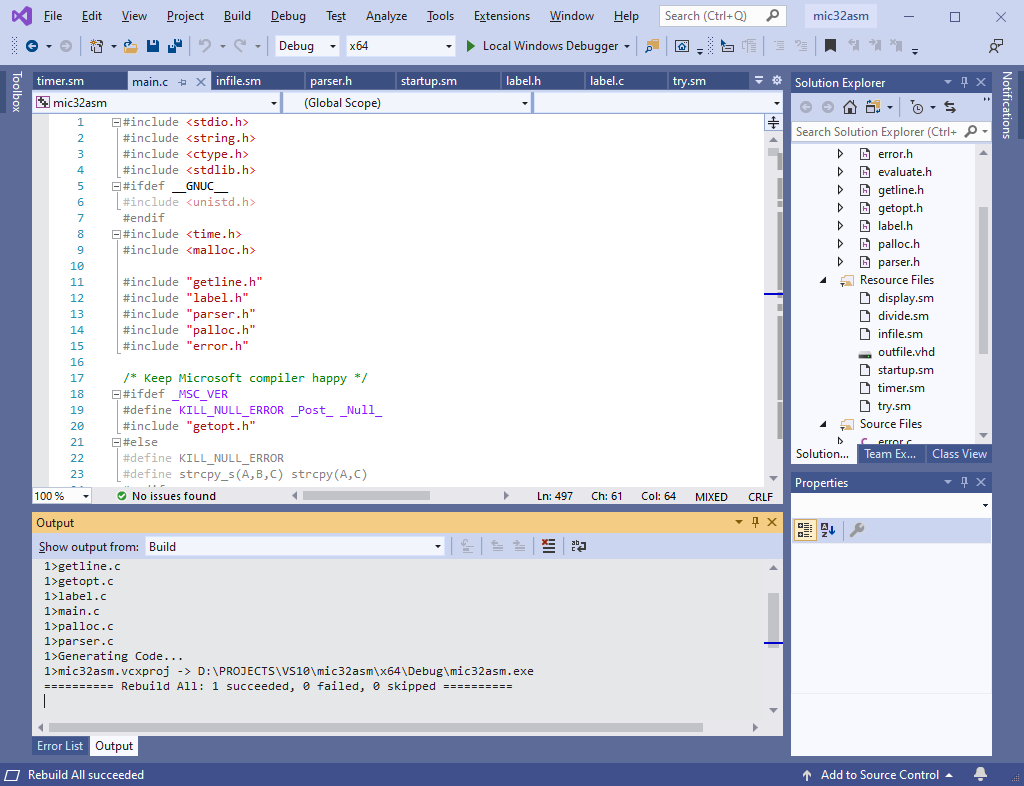
\includegraphics[width=\textwidth]{images/vs2019}
\caption{Voorbeeld van Microsoft Visual Stdio.}
\label{fig:unvs2019}
\end{figure}

We hebben nu een beeld van hoe op een computer een C-programma wordt vertaald naar instructies voor een computer. De computer kan het C-programma niet direct uitvoeren, het programma moet gecompileerd worden. Als we een wijziging in het C-programma willen doorvoeren, dan moeten we het C-programma uiteraard opnieuw compileren.

We zullen in de overige paragrafen in sneltreinvaart enkele concepten van C bespreken. In de volgende hoofdstukken wordt de taal verder uitgediept.


\section{Een minimaal C-programma}
We beginnen met het meest simpele C-programma dat mogelijk is. We willen hiermee uitleggen wat er gebeurt als dit programma gecompileerd en uitgevoerd wordt. Het programma is te zien in listing~\ref{cod:unminimaalcprogramma}. Het programma doet in feite helemaal niets, althans niet dat de gebruiker van het programma kan waarnemen. Toch gebeuren er wel degelijk dingen ``onder de motorkap''.

\begin{figure}[H]
\begin{lstlisting}[caption=Een minimaal C-programma.,label=cod:unminimaalcprogramma]
int main(void)
{
	return 0;
}
\end{lstlisting}
\end{figure}

Dit programma kan niet direct door de computer worden uitgevoerd, het moet eerst worden gecompileerd. Na compilatie is een \textsl{uitvoerbaar bestand}\index{uitvoerbaar bestand} beschikbaar dat wel door de computer kan worden uitgevoerd. De werking op een PC of laptop is als volgt. Als het uitvoerbare programma wordt gestart, dan zal het besturingssysteem het uitvoerbare programma in het geheugen van de computer laden. Dus ergens in het geheugen van de computer liggen de instructies die het programma vormen opgeslagen. Het besturingssysteem start het uitvoerbare programma door de processor naar de eerste instructie van het programma te leiden. Het programma (dat is het uitvoerbare programma) zal nu instructies uitvoeren. Na afloop van het programma wordt de besturing weer teruggeven aan het besturingssysteem.

Het C-programma begint met de definitie van de \textsl{functie} \texttt{main}\indextwo{main}{functie}. Een functie is een aantal instructies samengepakt onder een gemeenschappelijke noemer. \textsl{Elk C-programma heeft een functie \texttt{main}}. Tussen de haken staat het keyword \texttt{void}\indexkeyword{void}, dat aangeeft dat het uitvoerbaar programma geen gegevens meekrijgt van het besturingssysteem\footnote{Dat kan wel, zie hoofdstuk~\ref{cha:pointers}.}. Vóór \texttt{main} staat het keyword \texttt{int}\indexkeyword{int} dat aangeeft dat \texttt{main} een geheel getal teruggeeft aan het besturingssysteem.
 
Statements die in het C-programma gebruikt worden, zijn afgebakend met \textsl{accolades}\index{accolades}. Het Engelse woord hiervoor is \textsl{curly braces} of gewoon \textsl{braces}. De accolades geven het begin en einde aan van \textsl{blok}. Een blok begint met een accolade-openen (\texttt{\{}) en eindigt met een accolade-sluiten (\texttt{\}}). Over de plaats van de accolades zijn er diverse meningen. In listing~\ref{cod:unminimaalcprogramma} is de accolade-openen geplaatst onder de definitie van \texttt{main}, maar het is ook gebruikelijk om de accolade-openen te schrijven achter de definitie van \texttt{main}.
 
Binnen \texttt{main} zien we één \textsl{statement}\index{statement}. Een statement is een opdracht in de C-taal. Het statement wordt gevormd door het keyword \texttt{return}\indexkeyword{return} gevolgd door het getal 0 en een punt-komma. Bij uitvoering van dit statement wordt de waarde 0 teruggegeven aan het besturingssysteem. Dat behoeft enige uitleg. Een (gecompileerd) programma wordt gestart door het besturingssysteem. Aan het einde wordt het programma afgesloten. Het besturingssysteem ``ruimt'' het programma op en zorgt ervoor dat het gebruikte geheugen weer vrijgegeven wordt voor volgende programma's. We kunnen aan het besturingssysteem een getal teruggeven, in dit geval 0. Het is aan het besturingssysteem om hier wat mee te doen. Gebruikelijk is om 0 terug te geven als alles goed verlopen is. Een ander getal dan 0 geeft over het algemeen aan dat er iets fout gegaan is. Vanaf C99 is het niet meer nodig om dit \texttt{return}-statement uit te voeren. Dan wordt automatisch het getal 0 teruggegeven.

\section{Afdrukken op het scherm}
We kunnen het eerste programma interessanter maken door een regel tekst op het scherm af te drukken. Het programma in listing~\ref{cod:uneersteprogramma} drukt de regel \texttt{De som van 3 en 7 is 10} op het scherm af. We zullen het programma stap voor stap doorlopen.

\begin{figure}[!ht]
\begin{lstlisting}[caption=Afdrukken van de som van twee getallen.,label=cod:uneersteprogramma]
#include <stdio.h>

int main(void)
{
    int a = 3;
    int b = 7;

    int som;

    som = a + b;

	printf("De som van %d en %d is %d\n", a, b, som);

	return 0;
}
\end{lstlisting}
\end{figure}

In regel 1 wordt een zogenoemd \textsl{header-bestand}\index{header-bestand} geladen, in dit geval het bestand \texttt{stdio.h}\indextwo{stdio.h}{header-bestand}. We leggen zo meteen uit waarom dat nodig is.

In regel 3 wordt kenbaar gemaakt dat het programma de functie \texttt{main}\indextwo{main}{functie} heeft. Een C-programma heeft \textsl{altijd} de functie \texttt{main}. Het (gecompileerde) programma wordt hier gestart.

In regel 5 en 6 worden twee \textsl{variabelen}\index{variabele} gedeclareerd, de variabelen \texttt{a} en \texttt{b}. Technisch gezien is een variabele een plek in het geheugen van de computer. Een variabele kan door het programma gebruikt worden om gegevens te bewerken. Declaratie\index{declaratie} wil zeggen dat een variabele kenbaar wordt gemaakt. Bij de declaratie wordt opgegeven wat het type is van de variabele. Dit gebeurt middels het keyword \texttt{int}, dat betekent dat \texttt{a} en \texttt{b} alleen geheeltallige getallen kan opslaan (Engels: integer). Aan de variabelen worden gelijk waarden toegekend. We noemen dit \textsl{initialisatie}\index{initialisatie} van variabelen.

In regel 8 wordt de variabele \texttt{som} gedeclareerd zonder initialisatie. Dat betekent dat op dat moment de waarde (of inhoud) van de variabele \textsl{onbekend} is. Vervolgens wordt in regel 10 de som van \texttt{a} en \texttt{b} berekend middels de \textsl{optel-operator} \texttt{+}\indexop{+} en wordt het resultaat \textsl{toegekend}\index{toekenning}\indexop{=} aan variabele \texttt{som}. Vanaf regel 10 is de waarde van \texttt{som} dus 10. In regel 10 zien we zogenoemde \textsl{expressies}\index{expressie}. Zo is \texttt{a + b} een expressie en is de toekenning \mbox{\texttt{som = ...}} ook een expressie. De term expressie komt veel voor in C.

In regel 12 wordt de functie \texttt{printf}\indexfunc{printf} aangeroepen. Deze functie is al geschreven en zit in de standard library. De functie krijgt vier \textsl{argumenten}\index{argument} mee, gegevens die in de functie verwerkt worden. Het eerste argument is een \textsl{string}\index{string}. Een string is een stukje tekst, maar we spreken ook wel van een rij karakters. Daarna volgen de (waarden) van de variabelen \texttt{a}, \texttt{b} en \texttt{som}.

Het eerste argument van \texttt{printf} wordt een \textsl{format string} genoemd. Dat ligt niet in C-taal vast maar wordt algemeen gebruikt. De format string bevat karakters, zogenoemde \textsl{format specifications} en een \textsl{escape sequence}. Een format specification begint met een procentteken gevolgd door een letter. De functie \texttt{printf} gebruikt deze format specifications om de gegevens af te drukken. De eerste \texttt{\%d} zorgt ervoor dat variabele \texttt{a} wordt afgedrukt als een decimaal geheel getal. Op overeenkomstige wijze worden ook \texttt{b} en \texttt{som} afgedrukt. Aan het einde van de format string is een \textsl{escape sequence} te zien, in dit geval \texttt{\textbackslash n}. Dit zorgt ervoor dat een volgende afdruk wordt begonnen aan het begin van de volgende regel (Engels: newline).

In regel 14 wordt met het keyword \texttt{return} aangegeven dat het programma wordt afgesloten. 
Dat de return-waarde een geheel getal moet zijn, kunnen we zien aan de definitie van de functie \texttt{main}. We zien in regel 3 dat \texttt{main} een geheel getal teruggeeft (keyword \texttt{int}) en geen argumenten meekrijgt (keyword \texttt{void}).

Hoe weet de C-compiler nu hoe de functie \texttt{printf} moet worden aangeroepen? Dat wordt geregeld met een \textsl{function prototype}. We hoeven dat zelf niet op te geven want dat is al gedaan en is te vinden in het header-bestand \texttt{stdio.h}\indextwo{stdio.h}{header-bestand}. De eerste regel geeft dus aan dat dit bestand geladen moet worden. De tekens \texttt{<} en \texttt{>} geven aan dat gezocht moet worden op een bepaalde plek in het bestandssysteem. We hoeven dat verder niet te weten.

\section{Invoer van het toetsenbord}
We kunnen het vorige programma interessanter maken door aan de gebruiker te vragen om twee gehele getallen in te voeren. Naast het afdrukken van tekst met de functie \texttt{printf} maken we nu ook gebruik van de functie \texttt{scanf}\indextwo{scanf}{functie} om gehele getallen in te lezen. Het programma is te zien in listing~\ref{cod:unscanfprogramma}.

\begin{figure}[!ht]
\begin{lstlisting}[caption=Invoer van de gebruiker opvragen.,label=cod:unscanfprogramma]
#include <stdio.h>

/* Make Visual Studio happy */
#pragma warning(disable : 4996)

int main(void) 
{
    int a;
    int b;

    int som;

    printf("Geef een getal: ");
    scanf("%d", &a);

    printf("Geef nog een getal: ");
    scanf("%d", &b);

    som = a + b;

    printf("De som van %d en %d is %d\n", a, b, som);

    return 0;
}
\end{lstlisting}
\end{figure}

In regel 1 laden we weer het header-bestand \texttt{stdio.h}. Dit header-bestand is nodig om de functie-prototypes van \texttt{printf} en \texttt{scanf} te laden. In regel 4 maken we gebruik van een \textsl{pragma}\index{pragma}. Dit is een aanwijzing voor de C-compiler om iets te doen of te laten. Waarom deze pragma nodig is, kunnen we lezen in het kader.% op pagina~\pageref{fig:unopmerkingscanf}.

Het programma volgt verder de lijn van listing~\ref{cod:uneersteprogramma}. In de functie \texttt{main} declareren we drie variabelen. Daarna drukken we in regel 13 een stukje tekst af dat aangeeft wat de gebruiker moet doen. In regel 14 wordt de functie \texttt{scanf} aangeroepen die ervoor zorgt dat een geheel getal wordt ingelezen van het toetsenbord en in variabele \texttt{a} wordt gezet.

De format specification \texttt{\%d} hadden we al eerder gezien, maar de constructie \texttt{\&a} is nieuw. De ampersand (\texttt{\&}) zorgt ervoor dat aan de functie \texttt{scanf} het \textsl{adres} van variabele \texttt{a} meegegeven wordt. Het adres van de variabele is de plek waar de variabele in het geheugen ligt. Op deze manier kan \texttt{scanf} de informatie op je juiste plek zetten. In regel 17 wordt hetzelfde gedaan voor variabele \texttt{b}. We drukken voor het inlezen nog even netjes af hoe de gebruiker moet handelen. In regel 19 rekenen we de som uit van variabelen \texttt{a} en \texttt{b} en kennen dat toe aan variabele \texttt{som}. In regel 21 drukken we de drie variabelen af. Het programma wordt afgesloten in regel 23.

Als we het programma starten dan moeten we twee gehele getallen invoeren. Een mogelijke uitvoer van het programma is te zien in figuur~\ref{fig:unuitvoerprog}. De invoer van de gebruiker is vet afgedrukt.
Overigens zullen ontwikkelsystemen zoals Visual Studio aan het einde van het programma wachten tot de gebruiker op een toets drukt, anders is door de snelheid van het uitvoeren van het programma niet te zien wat is afgedrukt.

\begin{dosbox}[title=Uitvoer van het programma in listing~\ref{cod:unscanfprogramma}.,label=fig:unuitvoerprog]
Geef een getal: (*\textbf{7}*)
Geef nog een getal: (*\textbf{4}*)
De som van 7 en 4 is 11
\end{dosbox}

We hebben nu gezien hoe we invoer en uitvoer voor een programma kunnen gebruiken. In veel voorbeelden zullen we hiervan gebruik maken.

\begin{infobox}[To \texttt{scanf} or not to \texttt{scanf}...]
\label{fig:unopmerkingscanf}%
De Microsoft C-compiler bestempelt \texttt{scanf} als ``onveilig''. Een compilatie met \texttt{scanf} zal eindigen met een foutmelding. In plaats daarvan moet de functie \texttt{scanf\_s} worden gebruikt. Helaas ondersteunen andere compilers deze functie niet. Dat zal resulteren in een programma dat niet door iedere compiler kan worden vertaald. Om het probleem te omzeilen hebben we gebruik gemaakt van een \textsl{pragma}. In regel~4 geven we aan dat de C-compiler fout 4996 moet negeren. Op andere compilers, bijvoorbeeld de GNU-C compiler, wordt deze regel overgeslagen (er volgt wel een waarschuwing). Overigens wordt op vele fora gewaarschuwd voor de onveiligheid van \texttt{scanf} en worden alternatieven gegeven. Wij gebruiken \texttt{scanf} hier wel \textsl{for the sake of simplicity}. Het is beter om \texttt{scanf} te vermijden.
\end{infobox}

\section{Keywords}

In tabel~\ref{tab:unkeywords} is een lijst te zien met gereserveerde woorden. Een aantal van deze woorden hebben we algezien zoals \texttt{int}, \texttt{void} en \texttt{return}. Deze woorden worden \textsl{keywords}\index{keyword} genoemd en geven de compiler aanwijzingen over wat er moet gebeuren.

\begin{table}[!ht]
\caption{Een lijst met keywords in de C-taal.}
\label{tab:unkeywords}
\centering\ttfamily
\begin{tabular}{p{2.5cm}p{2.5cm}p{2.5cm}p{2.5cm}}
\toprule
auto &  double &  int & struct \\
break & else  & long  &  switch \\
case & enum & register & typedef \\
char & extern & return & union \\
const & float & short &  unsigned \\
continue & for & signed & void \\
default & goto & sizeof & volatile \\
do & if & static & while \\
\bottomrule
\end{tabular}
\end{table}

Een aantal van deze keywords dient als \textsl{qualifier}\index{qualifier} voor andere keywords. Zo kunnen we een variabele declareren als

\hspace*{1em}\texttt{unsigned long int a;}

Dit geeft de compiler aanwijzingen over de grootte (het aantal bits) van variabele \texttt{a}.


\section{Beslissingen}

Met behulp van de keyswords \texttt{if}\indexkeyword{if} en \texttt{else}\indexkeyword{else} kunnen we in het programma beslissingen nemen op basis van een \textsl{conditie}\index{conditie}. Dit is te zien in listing~\ref{cod:unif}. We declareren twee variabelen \texttt{a} en \texttt{b} en kennen gelijk de waarden 
%
\begin{figure}[!b]
\begin{lstlisting}[caption=Afdrukken van tekst op basis van een beslissing.,label=cod:unif]
#include <stdio.h>

int main(void)
{
    int a = 7;
    int b = 9;
    
    if (a < b)
    {
        printf("a is kleiner dan b\n");
    }
    
    return 0;
}
\end{lstlisting}
\end{figure}
%
toe. In regel 8 is te zien dat getest wordt of \texttt{a} kleiner is dan \texttt{b}. We noemen het kleiner-dan-teken een \textsl{relationele operator}\index{relationele operator}. Als inderdaad blijkt dat \texttt{a} kleiner is dan \texttt{b}, dat betekent dat de conditie \texttt{a < b} waar is, worden de statements tussen de accolades in de regels 9 en 11 uitgevoerd. Is de conditie niet waar, dan worden de regels overgeslagen. Overigens mogen in dit geval de accolades weggelaten worden omdat maar één statement wordt uitgevoerd. Het is echter aan te bevelen om ze toch te gebruiken, omdat misschien later er nog statements toegevoegd worden. Een bekend voorbeeld van het niet-gebruiken van accolades is Apple's \textsl{gotofail SSL security bug}~\cite{barr2014}.


Een \texttt{if}-statement kan ook gevolgd worden door een \texttt{else}-keyword en een \texttt{else}-keyword kan ook weer gevolgd worden door een \texttt{if}-keyword. In het Engels wordt dit een \textsl{multy-way branch} (to branch = vertakken) genoemd. Zie listing~\ref{cod:unifelse}.

\begin{figure}[!ht]
\begin{lstlisting}[caption=Afdrukken van tekst op basis van een beslissing.,label=cod:unifelse]
#include <stdio.h>

int main(void)
{
    int a = 7;
    int b = 9;
    
    if (a < b)
    {
        printf("a is kleiner dan b\n");
    }
    else if (a == b) 
    {
        printf("a is gelijk aan b\n");
    }
    else
    {
        printf("a is groter dan b\n");
    }
    return 0;
}
\end{lstlisting}
\end{figure}

Technisch gezien hoort de \texttt{else} in regel 16 bij de \texttt{if} in regel 12. Let erop dat het vergelijken van \texttt{a} en \texttt{b} op gelijkheid in regel 12 een \textsl{dubbele is-gelijk-teken} (\texttt{==})\indexop{==} bevat.

 
\section{Herhalingen}
Stel dat we de kwadraten van 1 t/m 10 willen afdrukken. We kunnen ervoor kiezen om tien \texttt{print}-functies aan te roepen. Maar we merken direct op dat we in feite tien keer hetzelfde moeten doen. We kunnen het afdrukken van de tien kwadraten vormgeven met een \textsl{herhaling}. Een andere, veel gebruikte term is \textsl{lus}\index{lus}. Dit is te zien in listing~\ref{cod:printkwadraten}.

\booklisting[]{C}{Afdrukken van de kwadraten van 1 t/m 10.}{printkwadraten}{c}{!ht}

We beginnen het programma met de declaratie van een aantal variabelen. Vervolgens stellen we de ondergrens, bovengrens en stapgrootte in in de regels 8 t/m 10. We willen beginnen bij de ondergrens, stoppen bij de bovengrens en bij elke herhaling nieuwe waarden afdrukken. Daarvoor gebruiken we de variabele \texttt{getal}. Zo'n variabele wordt een \textsl{lusvariabele}\index{lusvariabele} genoemd.

In regel 12 zetten we de lusvariabele op de ondergrens en gaan de lus uitvoeren. De lus wordt gekenmerkt door het keyword \texttt{while}\indexkeyword{while}. Achter het keyword \texttt{while} staat, tussen de haken, de conditie waarop de lus moet worden uitgevoerd.
Zolang de conditie \mbox{\texttt{getal <= bovengrens}} waar is, worden de statements binnen de accolades uitgevoerd. We noemen dat een \textsl{iteratie}\index{iteratie}. Is de conditie niet waar dan wordt verder gegaan met het statement die volgt op het \texttt{while}-statement.


Binnen de accolades van het \texttt{while}-statement zien we drie statements. In regel 15 wordt het kwadraat berekend van de (huidige) waarde van de lusvariabele. Daarna worden de lusvariabele en het kwadraat afgedrukt. In regel 17 wordt de lusvariabele aangepast naar de nieuwe (volgende) waarde door de stapgrootte erbij op te tellen\footnote{Het is tegenwoordig in het Nederlands gebruikelijk om het Engelse woord updaten te gebruiken.}.

In geval van het kwadratenprogramma kunnen we ook een ander herhalingsstatement gebruiken: het \texttt{for}-statement. Het is een compacte schrijfwijze van het \texttt{while}-statement. We kunnen het berekenen van het kwadraat ook als parameter van de functie \text{printf} plaatsen. Zo sparen we een variabele uit. Zie listing~\ref{cod:unfor}.

\begin{figure}[!ht]
\begin{lstlisting}[caption=Gebruik van een \texttt{for}-statement.,label=cod:unfor]
    // ...
	for (getal = ondergrens; getal <= bovengrens;
                                             getal = getal + stap)
	{
		printf("Het kwadraat van %3d is %3d\n",
                                             getal, getal*getal);
	}
    //...
\end{lstlisting}
\end{figure}


\section{Array's}
Een \textsl{array}\index{array} is een lijst variabelen onder een gemeenschappelijke noemer. Zo declareren we vijf floating point-getallen (getallen met een komma)\index{floating point} met

\hspace*{1em}\texttt{double lijst[5];}\indexkeyword{double}

en kunnen we gebruik maken van de variabelen

\hspace*{1em}\texttt{lijst[0] lijst[1] lijst[2] lijst[3] lijst[4]}

Tussen de blokhaken \texttt{[]}\indexop{[]} staat het \textsl{elementnummer} en de variabelen worden de \textsl{elementen} van de array genoemd. In listing~\ref{cod:arraygemiddelde} is een programma te zien met een array.

\booklisting[]{C}{Gemiddelde van vijf getallen}{arraygemiddelde}{c}{!ht}

De array mag bij declaratie gelijk geïnitialiseerd worden zoals te zien is in regel 5\footnote{We hebben als getallen vijf wiskundige constanten genomen. De lezer wordt uitgedaagd uit te zoeken welke constanten dat zijn.}. We berekenen van deze vijf elementen de gemiddelde waarde. We doen dat door eerst de som van de vijf element te berekenen en vervolgens te delen door 5. Met behulp van een \texttt{for}-statement wordt ``langs de array gelopen''; bij elke iteratie selecteren we een element en tellen dat op bij de som van de tot dan toe gesommeerde elementen. De regel

\hspace*{1em}\texttt{som = som + lijst[index];}

selecteert dus een element uit de array en telt dat op bij de som. In regel 13 drukken we het gemiddelde af door de som te delen door 5. We hoeven daarvoor niet een aparte variabele te declareren, we kunnen als argument gewoon \texttt{som / 5.0} gebruiken.

Een veel gebruikte arraytype is de \textsl{string}. Dit is een array van karakters, afgesloten met een speciaal karakter dat het \textsl{null-karakter} of \textsl{null-byte} genoemd worden. C heeft geen ingebouwde taalconstructies die direct met strings werken, maar er zijn veel \textsl{functies} beschikbaar om strings te verwerken. Een voorbeeld van een string is:

\begin{lstlisting}[caption=Voorbeeld van een string.]
char str[] = "Ik ben een string";
\end{lstlisting}

We hoeven de lengte van de string in dit geval niet op te geven, dat wordt automatisch door de C-compiler uitgerekend. Strings worden behandeld in hoofdstuk~\ref{cha:arrays}. 

% Past niet op pagina
%We kunnen de string bijvoorbeeld door het programma laten afdrukken met \lstinline|printf|:
%
%\begin{lstlisting}[caption=Afdrukken van een string.]
%    printf("%s", str);
%\end{lstlisting}

\section{Functies}
C biedt een handige manier om een groep statement, bijvoorbeeld berekeningen, onder te brengen in een \textsl{functie}\index{functie}. Als de functie eenmaal geschreven is hoeven we ons niet druk te maken over hoe de de berekeningen worden gedaan, we moeten alleen maar weten hoe we de functie moeten gebruiken. We hebben al drie functies gezien: \texttt{printf}, \texttt{scanf} en \texttt{main}. De functies \texttt{printf} en \texttt{scanf} zijn al beschikbaar via de standard library. We hoeven niet te weten hoe de functies werken, alleen maar hoe ze moeten worden aangeroepen.

Laten we eens de wortels bepalen van de getallen 0 t/m 10. Daartoe schrijven we een functie \texttt{sqrt\_babylonian} die de wortel van een getal bepaalt volgens de Babylonische methode. Dit is een iteratieve methode om de wortel van een getal steeds nauwkeuriger te benaderen. De manier waarop dat gebeurt is te zien in vergelijking~\eqref{equ:sqrtbab}.
%
\begin{equation}
\label{equ:sqrtbab}
\begin{split}
x_0 &= S &&&& \text{beginsituatie} \\
x_{n+1} &= \dfrac{1}{2}\cdot\left(x_n + \dfrac{S}{x_n}\right) &&&& \text{nieuwe situatie}\\
\sqrt{S} &= \lim_{n\rightarrow\infty} x_n &&&& \text{uiteindelijke resultaat}
\end{split}
\end{equation}
%
We lezen dit als volgt. We beginnen met het getal $S$ waarvan we de wortel willen berekenen ($x_0= S$). De tweede, iteratieve stap, is het berekenen van de volgende benadering. We berekenen dat met de middelste vergelijking uit~\eqref{equ:sqrtbab}. De laatste stap geeft aan dat als we de wortel willen bepalen, de tweede stap oneindig vaak herhaald moet worden. Natuurlijk is dat niet realiseerbaar. We kunnen maar een eindig aantal stappen uitrekenen. Het blijkt dat voor de wortel slechts tien stappen nodig zijn om de wortel redelijk te benaderen.

De functie is te zien in listing~\ref{cod:sqrt_babylonian}. We maken hier gebruik van het datatype \texttt{double}\indexkeyword{double}, een floating point-datatype met een nauwkeurigheid van ongeveer 16 decimale cijfers. Zowel het argument als het returnwaarde is van dit datatype. We beginnen met de functiedefinitie

\hspace*{1em}\texttt{double square\_root(double s)}

Binnen de functie maken we gebruik van de twee variabelen \texttt{xiter} en \texttt{i}. \texttt{xiter} wordt gebruikt om de nieuwe waarde van de wortel te berekenen en \texttt{i} wordt gebruik om het aantal iteraties bij te houden.
We testen in regels 8 t/m 10 of het argument 0 is en geven dan direct de waarde 0 terug.

\booklisting[]{C}{Programma om de wortels van 1 t/m 10 af te drukken}{sqrt_babylonian}{c}{!ht}

In het \texttt{for}-statement worden tien iteraties van de middelste formule uit~\eqref{equ:sqrtbab} uitgevoerd. Bij elke iteratie wordt de waarde van de wortel steeds beter benaderd. Als het \texttt{for}-statement klaar is, wordt deze waarde via \texttt{return} teruggegeven aan de aanroeper. In \texttt{main} worden met behulp van een \texttt{for}-statement de wortels van 0 t/m 10 berekend en afgedrukt.

Overigens bevat de \textsl{mathematical library} een implementatie van de wortel-functie. We hoeven dat niet zelf te schrijven. Functies worden behandeld in hoofdstuk~\ref{cha:functies}.


\section{Programmeerstijlen}
C is erg coulant in het vormgeven van een programma. Het maakt meestal niet uit waar we de statements zetten en hoe een groep statements worden afgebakend. We kunnen regels overslaan (een lege regel) en we kunnen statements vooraf laten gaan door een willekeurig aantal spaties of we kunnen statements achter elkaar op een regel plaatsen.
Ook het gebruik van variabelenamen en functienamen staat geheel los van de taal. We kunnen één letter gebruiken of een compleet woord.

Een mooi voorbeeld hoe we onze wortelfunctie onleesbaar kunnen maken, kunnen we zien in listing~\ref{cod:sqrt_babylonian_bad_style}. De functie wordt door de C-compiler correct vertaald maar is voor een mens slecht leesbaar. De code in listing~\ref{cod:sqrt_babylonian} is veel beter leesbaar.

\booklisting[]{C}{Een functie om een wortel van een getal te bepalen}{sqrt_babylonian_bad_style}{c}{!ht}

Hoe een programma uiterlijk wordt vormgegeven noemen we een \textsl{programmeerstijl}\index{programmeerstijl}. Er zijn behoorlijk wat stijlen. We geven hieronder de meest gebruikte aan.

\subsubsection*{Layout van het programma}
In de K\&R-stijl (Kernighan en Ritchie)\index{K\&R-stijl} wordt de accolade-openen \textsl{achter} een functie, beslis-sings- of herhalingstatement geschreven. De statements hierbinnen worden \textsl{ingesprongen} (dat wordt in het Engels \textsl{indentation} genoemd)\index{inspringen!van code}\index{indentation}. Bij gebruik van in elkaar verweven beslissings- of herhalingstatement worden de statements verder of dieper ingesprongen. 
\begin{lstlisting}[caption=K\&R-stijl.]
while (a < b) {
    (*\normalfont\textsl{statements}*)
    if (a < 0) {
        (*\normalfont\textsl{statements}*)
    }
}
\end{lstlisting}

In de Allman-stijl\index{Allman-stijl} wordt de accolade-openen \textsl{onder} een functie, beslissings- of herhalingstatement geschreven. De statement hierbinnen worden \textsl{ingesprongen}. Bij gebruik van in elkaar verweven beslissings- of herhalingstatement worden de statement verder of dieper ingesprongen.

\begin{lstlisting}[caption=Allman-stijl.]
if (a < b)
{
    if (a < 0)
    {
        (*\normalfont\textsl{statements}*)
    }
}
\end{lstlisting}

\subsubsection*{Naamgeving van variabelen}

Ook voor naamgeving van variabelen zijn diverse gebruiken in omloop. We zullen er drie behandelen.

In de K\&R-stijl zijn er eigenlijk geen regels. Variabelennamen mogen uit één letter bestaan, of natuurlijk uit meerdere letters. Als namen syntactisch uit meerdere woorden bestaan, worden de woorden gescheiden door een \textsl{underscore}.\index{underscore} Het is wel aan te raden dat namen zinvol zijn en dat ze de betekenis vertegenwoordigen. Overigens is het gebruik van eenletterige variabelennamen prima te verantwoorden, bijvoorbeeld binnen het gebruik van een kortduurdende herhaling én als het programma niet al te groot is\footnote{In dit boek gebruiken we vooral de K\&R-stijl. We gebruiken ook vaak eenletterige variabelen. Dat is te verklaren omdat veel voorbeelden kort zijn en we de lezer niet willen vermoeien met lange variabelennamen.}.

In de camelCase-stijl worden variabelen weergegeven met kleine letters en hoofdletters en geven scheidingen aan tussen woorden die syntactisch gescheiden zijn. Er worden geen underscores gebruikt. Deze stijl is afkomsting uit Java.

\begin{lstlisting}[caption=camelCase-stijl.]
    int dayOfTheWeek;
    int dayWithinMonth;
    int dayOfTheYear;
\end{lstlisting}

Bij de Hungarian Notation worden variabelennamen vooraf gegaan door een omschrijving van het datatype en het semantiek van de variabele. Zo kunnen we integers vooraf laten kunnen gaan door een \lstinline|i|. Maar dat zien de meeste programmeurs ook wel. We kunnen van een integer ook het doel aangeven. Zo wordt bijvoorbeeld een variabele die dient als teller in een herhaling vooraf gegaan door \lstinline|c| (van ``count''):

\begin{lstlisting}[caption=Voorbeel Hungarian Notation.]
    int iDayOfTheWeek;
    int cLoops;
\end{lstlisting}

Deze stijl wordt vooral gebruikt bij grote teams programmeurs zie gezamenlijk aan één programma werken. Het nadeel van deze stijl is dat de typering niet gestandaardiseerd is.

\section{En verder...}
We hebben nu enkele concepten van C uitgelegd. Maar de taal kan meer. Wat we niet behandeld hebben zijn \textsl{pointers} en \textsl{structures}, onderdelen van de taal. We hebben ook \textsl{bestandsverwerking} niet behandeld. Dit is technisch gezien geen onderdeel van de taal, maar wordt vaak gebruikt in programma's. Al deze concepten zullen in de volgende hoofdstukken worden uitgelegd.

\chapter{Variabelen, datatypes en expressies}
\label{cha:vardatexp}
\thispagestyle{empty}

Een C-programma bestaat uit variabelen en functies. We gebruiken variabelen om data te bewerken, zoals berekenen van nieuwe waarden of testen of twee variabelen aan elkaar gelijk zijn. De compiler moet notie hebben welke variabelen in een programma gebruikt worden en hoe groot de variabelen zijn. De meeste moderne computersystemen werken met 64-bits eenheden en dat betekent dat een variabele een bepaald bereik heeft; niet elk getal kunnen we in een variabele opslaan.
We gebruiken functies om bewerkingen op de variabelen te beschrijven. We hebben al één functie gezien: \texttt{main}. Functies worden in detail besproken in hoofdstuk~\ref{cha:functies}.


\section{Variabelen}
Een \textsl{variabele}\index{variabele} is een object waaraan een waarde kan worden toegekend. Technisch gezien is een variabele een plek in het geheugen van een computer. Een variabele moet in het C-programma kenbaar gemaakt worden. We noemen dat de \textsl{declaratie}\index{declaratie} van de variabele. Bij de declaratie wordt het \textsl{type} van de variabele opgegeven. Zo geeft de declaratie

\hspace*{1em}\texttt{int a;}

aan dat in het programma de variabele \texttt{a} wordt gebruikt van het type \texttt{int}. Een \texttt{int} is een geheeltallig getal; het Engelse woord hiervoor is \textsl{integer}\index{integer}. Getallen met een komma, zoals~$3,14159$, kunnen we niet in een \texttt{int} opslaan. We kunnen nu in het programma de waarde van de variabele vastleggen met een \textsl{toekenning}\index{toekennen}. In het Engels is dat een \textsl{assignment}.\index{assignmemt} Als we aan \texttt{a} de waarde 2 willen toekennen dan schrijven we

\hspace*{1em}\texttt{a = 2;}

De C-compiler zorgt ervoor dat in het geheugen van de computer ruimte wordt gereserveerd om de variabele op te slaan. Als we in een programma de variabele \texttt{a} gebruiken dan weet de compiler op welk geheugenadres hij moet zoeken. We mogen de variabele onbeperkt aantal keer aanpassen. Zo kunnen we schrijven:

\begin{figure}[!ht]
\begin{lstlisting}[caption=Meerdere toekenningen aan een variabele.]
int a;
...
a = 2;
...
a = -3;
...
a = 5;
\end{lstlisting}
\end{figure}

De naam van de variabelen mag 31 karakters lang zijn. Er is geen noodzaak (en zelfs \textsl{bad practice}) om namen uit één karakters te laten bestaan. Hoofdletters en kleine letters zijn \textsl{niet} gelijk aan elkaar dus \texttt{count} is niet hetzelfde als \texttt{COUNT}. Dit wordt kast-ongevoelig\index{kast-ongevoelig} genoemd. Overigens accepteren C-compilers langere namen dan 31 karakters.

Er zijn enkele regels aan de namen van variabelen:

\begin{itemize}
\item Moet beginnen met een letter;
\item Mag alleen letters, cijfers en de underscore\index{underscore} bevatten;
\item Mag geen keyword zijn;
\item Mag geen bekende functienaam zijn;\footnote{Dat mag wel, maar dan kunnen we de functie niet in een programma gebruiken. We kunnen dus schrijven \texttt{int printf;} maar dan kan de \texttt{printf}-functie niet aangeroepen worden.}
\item Mag niet eerder gedeclareerd zijn;
\end{itemize}

Enkele goede voorbeelden:

\hspace*{1em}\texttt{Count}\quad\texttt{val23}\quad\texttt{loop\_counter}\quad\texttt{ary2to4}

Enkele foute voobeelden:

\hspace*{1em}\texttt{\_loop}\quad\texttt{50cent}\quad\texttt{int}\quad\texttt{printf}

De meeste C-compilers accepteren de underscore als eerste karakter. Dit wordt echter afgeraden omdat veel \textsl{systeemroutines} de underscore als eerste karakter gebruiken en dat kan problemen geven in de latere stadia van de compilatie (zie hoofdstuk~\ref{cha:compilatieproces}).

Bij de declaratie van variabelen mogen ook gelijk waarden worden toegekend, op voorspraak dat de waarden constant zijn. Een voorbeeld is hieronder te zien:\index{initialisatie}

\hspace*{1em}\texttt{int a = 2;}\\
\hspace*{1em}\texttt{int b = 3+5;}

\section{Datatypes}
Een variabele is van een bepaald \textsl{datatype}\index{datatype}. We hebben er al één gezien, de \texttt{int}. Een datatype heeft een bepaalde grootte. Zo bestaat een \texttt{int} \textsl{meestal} uit 32 bits. Er zijn echter ook systemen en C-compilers waar een \texttt{int} uit 16 bits bestaat. Dat een \texttt{int} uit 32 bits bestaat, betekent dat niet elk willekeurig getal aan de \texttt{int} kunnen worden toegekend. Er is een minimale en maximale waarde. Voor de \texttt{int} is de minimale waarde $-2147483648$ en de maximale waarde $+2147483647$. De \texttt{int} is een \textsl{signed} datatype: zowel positieve als negatieve getallen en 0 zijn mogelijk.

Nu is de grootte van een \texttt{int} niet altijd noodzakelijk of toereikend in een bepaalde situatie. We kunnen dan kiezen voor een ander type. C kent een aantal geheeltallige datatypes van diverse grootten. Deze zijn weergegeven in tabel~\ref{tab:varintdatatypes}.

\begin{table}[!ht]
\centering
\caption{De signed dataypes die beschikbaar zijn in C.}
\label{tab:varintdatatypes}
\begin{tabular}{@{}lcc@{}}
\toprule
\textbf{type}          & \textbf{bits} & \textbf{bereik}  \\ \midrule
\texttt{char}          & 8                       & $-128$ --- $+127$  \\
\texttt{short int}     & 16                      & $-32768$ --- $+32767$ \\
\multirow{2}{*}{\texttt{int}}   & 16                      & $-32768$ --- $+32767$ \\
                       & 32                      & $-2147483648$ --- $+2147483647$ \\
\texttt{long int}      & 32                      & $-2147483648$ --- $+2147483647$  \\
\texttt{long long int} & 64                      & $-9223372036854775808$ --- $+9223372036854775807$  \\
%\texttt{float}         & 32                      &                  \\
%\texttt{double}        & 64                      &                  \\
   \bottomrule
\end{tabular}
\end{table}

\indexkeyword{int}\indexkeyword{char}\indexkeyword{short}\indexkeyword{long}\indexkeyword{long long}
Een \texttt{char} wordt gebruikt om een karakter op te slaan en is 8 bits groot. De interpretatie van het opgeslagen karakter is afhankelijk van de computer waarom het programma draait. Merk op dat een \texttt{char} zowel negatieve als positieve waarden kan bevatten. De meest gebruikte codering is de ASCII-code. Om het karakter `A' op te slaan schrijven we:

\hspace*{1em}\texttt{char karak;}\\
\hspace*{1em}\texttt{karak = \textquotesingle A\textquotesingle; \ \ \ /* assign character A */}

Nu is de C-compiler erg coulant in het toekennen van waarden. We mogen voor de toekenning ook een getal gebruiken. We kunnen het bovenstaande ook schrijven als:

\hspace*{1em}\texttt{char karak;}\\
\hspace*{1em}\texttt{karak = 65; \ \ \ /* assign character A */}

Uiteraard moet de waarde passen en we merken terloops op dat negatieve waarden geen echte karakters voorstellen. Een \texttt{short int} is meestal 16 bits. Een \texttt{int} is 16 of 32 bits groot afhankelijk van de gebruikte C-compiler en de onderliggende hardware. Een \texttt{long int} is 32 bits. De C-standaard legt vast dat:

\hspace*{1em}grootte \texttt{short int} $\quad\leq\quad$ grootte \texttt{int} $\quad\leq\quad$ grootte \texttt{long int}

De keywords \texttt{short} en \texttt{long} worden \textsl{qualifiers}\index{qualifier} genoemd. Bij gebruik hiervan mag \texttt{int} weggelaten worden:

\hspace*{1em}\texttt{short sh; \ \ \ /* short int */}\\
\hspace*{1em}\texttt{long lo; \ \ \ \ /* long int */}

Als we aan een integer alleen maar positieve waarden of 0 toekennen dan kunnen we de qualifier \texttt{unsigned}\index{unsigned} bij declaratie opgeven. Het (positieve) bereik is dan ongeveer twee keer zo groot als bij de signed variant:

\hspace*{1em}\texttt{unsigned short int ush; \ \ \ /* range 0 to 65535 */}

Naast geheeltallige datatypes kent C ook een drietal \textsl{floating point} datatypes\index{floating point}. Het Nederlandse woord hiervoor is \textsl{drijvende komma}. Hier ontstaat al gelijk de eerste verwarring: in C wordt de komma vervangen door de punt, zoals gebruikelijk is in Engelstalige literatuur. We schijven dus $3.14$ en niet $3,14$.

Een \texttt{float}\indexkeyword{float} is een datatype met een grootte van 32 bits. Een \texttt{double}\indexkeyword{double} is een datatype met een grootte van 64 bits. We zouden verwachten dat de \texttt{long double}\indexkeyword{long double} dan een datatype van 128 bits is, maar dat is niet altijd waar. De \texttt{long double} is soms ook 80 bits, bijvoorbeeld in Intel-processoren.

\begin{table}[!ht]
\centering
\caption{De floating point dataypes die beschikbaar zijn in C.}
\label{tab:varfloatdatatypes}
\begin{tabular}{@{}lccc@{}}
\toprule
\textbf{type}          & \textbf{bits} & \textbf{kleinste getal} &  \textbf{grootste getal} \\ \midrule
\texttt{float}         & 32                      & $\approx1,18\times10^{-38}$ & $\approx3,4\times10^{38}$  \\
\texttt{double   }     & 64                      & $\approx2.2\times10^{-308}$ & $\approx1.8\times10^{308}$ \\
\texttt{long double}   & 80/128                      & $^1$) & $^1$)  \\
\bottomrule
\end{tabular}\\\vspace*{1mm}
\footnotesize$^1$) Afhankelijk van de implementatie 80 of 128 bits.
\end{table}

Voorbeelden van floating point variabelen:

\hspace*{1em}\texttt{float f;}\\
\hspace*{1em}\texttt{double d;}

Met betrekking tot de nauwkeurigheid kunnen we nog het volgende vermelden. Een \texttt{float} heeft een nauwkeurigheid van ongeveer 6 decimale cijfers. Het heeft dus geen zin om meer cijfers toe te voegen, de extra cijfers worden genegeerd. Een \texttt{double} heeft een nauwkeurigheid van ongeveer 16 decimale cijfers. Niet alle getallen kunnen exact in een floating point-variabele worden opgeslagen. Zo is 1/7 niet exact te representeren. Bij veelvuldig rekenen met floating point-variabelen treedt er verlies op in de representatie. Als we bijvoorbeeld 1/3 met 3 vermenigvuldigen, kan het zijn dat het resultaat 0,99999 is en niet 1,0. De floating-point weergave maakt het mogelijk om een breed dynamisch bereik van waarden te bestrijken met een constant aantal significante cijfers.

Al deze datatypes worden \textsl{enkelvoudige datatypes}\index{enkelvoudige datatypes} genoemd. Dat betekent dat de compiler ze ziet als één eenheid. Het is niet mogelijk om enkelvoudige datatypes te splitsen over meerdere andere datatypes.

Naast de genoemde datatypes bestaat er nog een datatype: de \textsl{pointer}\index{pointer}. Een pointer is een variabele die het \textsl{adres}\index{adres} bevat van een (andere) variabele. Pointers worden in detail besproken in hoofdstuk~\ref{cha:pointers}.


\section{Constanten}
\index{constante}
Een geheeltallige constante zoals \texttt{123} is van het type \texttt{int}. Door er een \texttt{L} achter te zetten wordt de constante een \texttt{long}. Dus \texttt{123L} is een \texttt{long}. Als een constante te groot is voor een \texttt{int} wordt het automatisch gezien als een \texttt{long}. Een unsigned constante wordt aangegeven met een \texttt{U} aan het einde. Dat mag in combinatie met de \texttt{L}. Een floating point-constante bestaat uit cijfers, optioneel met een punt. Dus \texttt{1.23} is een floating point-constante. Om 10-machten aan te geven wordt de $E$-notatie gebruikt. Zo staat \texttt{125.0E-3} voor $0,125$. Een floating point-constante is automatisch van het type \texttt{double}, tenzij er een \texttt{F} aan het einde staat, dan is de constante van het type \texttt{float}.

Geheeltallige constanten kunnen op drie manieren worden ingevoerd: als decimaal getal, als octaal getal of als hexadecimaal getal. Een constante die begint met \texttt{0} wordt gezien als octaal getal. Een octaal getal bestaat alleen uit de cijfers 1 t/m 7. Een constante die begin met de \textsl{prefix}\index{prefix} \texttt{0x} of \texttt{0X} wordt gezien als een hexadecimaal getal. Een constante die begint met de cijfers \texttt{1} t/m \texttt{9} wordt gezien als een decimaal getal.

\hspace*{1em}\texttt{int a = 0377; \ \ \ /* octal 377 is decimal 255 */}\\ 
\hspace*{1em}\texttt{int b = 0xa9; \ \ \ /* hexadecimal A9 is decimal 169 */}\\ 
\hspace*{1em}\texttt{int c = 127; \ \ \ \ /* decimal 127 */}

De C-standaard kent geen manier om binaire getallen in te voeren. Veel compilers ondersteunen dit toch door de prefix \texttt{0b} te gebruiken. Zo is de constante \texttt{0b10101001} gelijk aan~169.

Een\textsl{ karakterconstante}\index{karakterconstante} is een geheel getal, geschreven als een één karakter tussen apostrofes. Zo is \texttt{\textquotesingle A\textquotesingle} een karakterconstante. De interne representatie is een geheel getal dat overeen komt met de karakterset van de computer. Over het algemeen wordt de ASCII-code gebruikt en komt \texttt{\textquotesingle A\textquotesingle} overeen met de waarde 65.
De standaard ASCII-tabel is te vinden in bijlage~\ref{cha:asciitabel}.

Niet alle karakters kunnen zo worden ingevoerd. Een voorbeeld is het karakter \texttt{'} zelf. Om dit karakter in te voeren gebruiken we een \textsl{escape sequence}\index{escape sequence}. Een escape sequence bestaat uit een \textsl{backslash}\index{backslash karakter} (\texttt{\textbackslash}) en een karakter. We kunnen de apostrofe dus voorstellen met \texttt{\textquotesingle\textbackslash\textquotesingle\textquotesingle}.

De C-standaard kent een hele verzameling van dit soort escape sequences. Eén daarvan hebben we al meerdere malen gezien: de newline. Deze wordt aangegeven met \texttt{\textquotesingle\textbackslash n\textquotesingle}. Een aantal escape sequences is vermeld in tabel~\ref{tab:varescseq}.

\begin{table}[!ht]
\centering
\caption{Enkele escape sequences in C.}
\label{tab:varescseq}
\begin{tabular}{llp{1cm}ll}
\toprule
\texttt{\textbackslash n} & \texttt{n}ewline         &  & \texttt{\textbackslash\textbackslash}  & backslash \\
\texttt{\textbackslash r} & carriage \texttt{r}eturn &  & \texttt{\textbackslash\textquotesingle} & single quote \\
\texttt{\textbackslash a} & \texttt{a}udible bell    &  & \texttt{\textbackslash "} & double quote \\
\texttt{\textbackslash b} & \texttt{b}ackspace       &  & \texttt{\textbackslash 0} & null byte \\
\texttt{\textbackslash f} & \texttt{f}ormfeed        &  & \texttt{\textbackslash t} & horizontal \texttt{t}ab \\
\bottomrule
\end{tabular}
\end{table}

\indextwo{\textbackslash n}{newline karakter}\index{newline}
\indextwo{\textbackslash r}{carriage return karakter}\index{carriage return}
\indextwo{\textbackslash \textbackslash }{backslash karakter}\index{backslash}
\indextwo{\textbackslash 0}{nul-karakter}
\indextwo{\textbackslash t}{horizontal tab karakter}\index{horizontal tab}

Andere karakters kunnen worden gevormd door de backslash, gevolgd door de letter \texttt{x} en één of twee hexadecimale cijfers. We kunnen de letter \texttt{A} dus ook schrijven als \texttt{\textquotesingle\textbackslash x41\textquotesingle}.

Een \textsl{string constante}\index{string constante}, of kortweg string\index{string}, is een rij van karakters die wordt begonnen en afgesloten met aanhalingstekens. De rij mag ook leeg zijn. Dan spreken we dan van een lege string. Twee voorbeelden:

\hspace*{1em}\texttt{"Dit is een string"}\\
\hspace*{1em}\lstinline[basicstyle=\ttfamily]|""|\texttt{\ \  /* The empty string*/}

Let erop dat een string \textsl{geen} enkelvoudig datatype is zoals \texttt{int} en \texttt{double}. Een string is een rij karakters die in het geheugen liggen. Technisch gezien is een string een \textsl{array}\index{string array}. We kunnen dus niet de waarde van een string bepalen zoals dat wel mogelijk is van een \texttt{int} of een \texttt{char}. Aan het einde van een string wordt automatisch een nul-karakter\index{nul-karakter} geplaatst. Er is dus altijd één karakter meer nodig dan het aantal karakters in een string. In figuur~\ref{fig:varstrings} zijn de twee strings afgebeeld. De \texttt{\textquotesingle\textbackslash0\textquotesingle} stelt het nul-karakter voor.

\begin{figure}[!ht]
\centering
\begin{tikzpicture}[pointerstyle]
\foreach \ii [count=\i from 0] in {D, i, t, \ , i, s, \ ,e, e, n, \ , s, t, r, i, n, g, \textbackslash 0} {
	\node[memlocarray] (nod\i) at (\i*\unitsize,0) {\ii};
	\draw (nod\i) node[yshift=\unitsize cm] {\footnotesize\i}; 
}
\foreach \ii [count=\i from 0] in {\textbackslash 0} {
	\node[memlocarray] (nod\i) at (\i*\unitsize+7,-2) {\ii};
	\draw (nod\i) node[yshift=\unitsize cm] {\footnotesize\i}; 
}
\end{tikzpicture}
\caption{Uitbeelding van twee strings.}
\label{fig:varstrings}
\end{figure}

C kent geen ingebouwde operaties op strings, zoals inkorten, aan elkaar plakken, kopiëren of lengte bepalen. Dit moet allemaal door de programmeur zelf ontworpen worden. Gelukkig kent de standard library een groot aantal functies voor het bewerken van strings. We komen hierop terug in hoofdstuk~\ref{cha:arrays}.

Bij de declaratie van variabelen mogen ook gelijk waarden worden toegekend, op voorspraak dat de waarden constant zijn. De constante waarde mag ook berekend worden. Een aantal voorbeelden is hieronder te zien:

\hspace*{1em}\texttt{int a = 2;}\\
\hspace*{1em}\texttt{char z = \textquotesingle z\textquotesingle;}\\
\hspace*{1em}\texttt{short a = -10+5;}\\
\hspace*{1em}\texttt{long l = 123L;}\\
\hspace*{1em}\texttt{float tau = 2.0F*3.14159F;}\\
\hspace*{1em}\texttt{double e = 2.718281828;}\\
\hspace*{1em}\texttt{double googol = 1E100;}\\
\hspace*{1em}\texttt{unsigned char = 128+127;}

Let erop dat de constante wordt geconverteerd naar het type van de variabele. Sommige compilers geven een waarschuwing als zo'n conversie plaatsvindt.

\hspace*{1em}\texttt{int a = 25.6; \ \ /* converted to 25 */}\\
\hspace*{1em}\texttt{float b = 7; \ \ \ /* converted to 7.0 */}

Bij de declaratie van een variabele mag de qualifier \texttt{const}\indexkeyword{const} worden opgegeven dat inhoudt dat aan  de variabele eenmalig een waarde wordt toegekend. De \texttt{const}-variabele kan daarna niet meer veranderen. Dat is bijzonder handig als we een constante waarde moeten gebruiken in een programma. Zo kunnen we na de declaratie

\hspace*{1em}\texttt{const int aantal = 10;}

de variabele \texttt{aantal} gebruiken als vervanging voor het getal 10. Als later blijkt dat het aantal moet worden aangepast, dan hoeven we alleen maar de variabele \texttt{aantal} aan te passen.

Uiteraard moet de constante passen. Als we bijvoorbeeld

\hspace*{1em}\texttt{char ch = 65536;}

uitvoeren zal de compiler een waarschuwing geven dat de constante niet past in een \texttt{char}.


\section{Expressies}
\index{expressie}
Een \textsl{expressie} is elk stukje programma dat een uitkomst oplevert. Zo is \texttt{2+2} een expressie die de waarde 4 oplevert. We kunnen de uitkomst van een expressie toekennen aan een variabele. De toekenning zelf is ook een expressie:

\hspace*{1em}\texttt{a = 2 + 2;}

Een expressie mag variabelen bevatten:

\hspace*{1em}\texttt{a = b - c;}

Zelfs de regel

\hspace*{1em}\texttt{a;}

is een expressie die 4 oplevert als de waarde van \texttt{a} 4 is. Ook het vergelijken van twee variabelen is een expressie en mag toegekend worden aan een variabele:

\hspace*{1em}\texttt{a = b == c; \ \ \  /* note the == */}

Als \texttt{b} gelijk is aan \texttt{c} dan wordt \texttt{a} gelijk aan 1. Als \texttt{b} ongelijk is aan \texttt{c} dan wordt \texttt{a} gelijk aan~0. We zullen het vergelijken van variabelen en constanten nader bekijken in hoofdstuk~\ref{cha:programmabesturing}.

Een expressie mag willekeurig complex zijn, maar let op de voorrangsregels: vermenigvuldigen en delen gaan voor op optellen en aftrekken. Haakjes worden gebruikt de prioriteiten te veranderen:

\hspace*{1em}\texttt{a = (2+b)*5+c;}

\subsection{Rekenkundige operatoren}
C kent vijf \textsl{binaire} rekenkundige operatoren: \texttt{*}\indextwo{*}{vermenigvuldigen} voor vermenigvuldigen, \texttt{/}\indextwo{/}{delen} voor delen, \texttt{\%}\indextwo{\%}{modulus operator} voor de modulus, \texttt{+}\indextwo{+}{optellen} voor optellen en \texttt{-}\indextwo{$-$}{aftrekken} voor aftrekken. Binair wil in dit verband zeggen dat de operatoren op twee variabelen (of constanten of expressies) werken. 
%De \textsl{binaire} rekenkundige operatoren zijn \texttt{*}\indextwo{*}{vermenigvuldigen}, \texttt{/}\indextwo{/}{delen}, \texttt{\% }\indextwo{\%}{modulus operator}, \texttt{+}\indextwo{+}{optellen} en \texttt{-}\indextwo{$-$}{aftrekken}. Binair wil in dit verband zeggen dat de operatoren op twee variabelen (of constanten of expressies) werken.
De expressie

\hspace*{1em}\texttt{a \% b}

berekent de rest van de deling van \texttt{a} gedeeld door \texttt{b}. Dit wordt de \textsl{modulus operator}\index{modulus operator} genoemd. Deze operator mag alleen op geheeltallige getallen gebruikt worden. Daarnaast kunnen \texttt{+} en \texttt{-} ook als \textsl{unaire operator}\index{unaire operator} gebruikt worden. Een voorbeeld hiervan is

\hspace*{1em}\texttt{int a = -5;}

Let goed op de prioriteiten van de operatoren. De unaire operatoren gaan voor op vermenigvuldigen (\texttt{*}), delen (\texttt{/}) en modulus (\texttt{\%}). De binaire optelling (\texttt{+}) en aftrekking (\texttt{-}) hebben en lagere prioriteit dan \texttt{*}, \texttt{/} en \texttt{\%}. Haakjes kunnen de volgorde veranderen. Merk op dat de \textsl{associativiteit}\index{associativiteit} van deze operatoren van links naar rechts is. Dus de expressie

\hspace*{1em}\texttt{a / b / c}

is equivalent aan

\hspace*{1em}\texttt{(a / b) / c}
 
maar \textsl{niet} aan

\hspace*{1em}\texttt{a / (b / c)}

Verder moet worden opgelet bij deling van geheeltallige getallen. Een deling rondt naar beneden af, dus de \textsl{fractie}\index{fractie}, het deel van een getal na de komma, wordt weggelaten. Dat betekent dat

\hspace*{1em}\texttt{1 / 3 * 3}

de waarde 0 oplevert. Eerst wordt 1/3 berekend en de geheeltallige uitkomst hiervan is 0. Daarna wordt de uitkomst met 3 vermenigvuldigd. De uitkomst is nog steeds 0.

\subsection{Relationele operatoren}
De zes \textsl{relationele operatoren}\index{relationele operatoren} zijn

\hspace*{1em}\texttt{==} \quad \texttt{!=} \quad \texttt{>} \quad \texttt{>=} \quad \texttt{<} \quad \texttt{<=}

\indexop{==}\indexop{"!=}\indexop{>}\indexop{>=}\indexop{<}\indexop{<=}
Hierin zijn \texttt{==} gelijk aan en \texttt{!=} ongelijk aan. Verder is \texttt{>} groter dan, \texttt{>=} is groter dan of gelijk aan, \texttt{<} is kleiner dan en \texttt{<=} is kleiner dan of gelijk aan. Deze hebben een lagere prioriteit dan de alle rekenkundige en unaire operatoren, dus \texttt{i < len-1} wordt gelezen als \texttt{i < (len-1)}. Overigens hebben \texttt{==} en \texttt{!=} een lagere prioriteit dan de overige vier. Een relationele operator levert de waarde 1 op als de vergelijking waar is en anders levert de relationele operator~0 op.
De relationele operatoren hebben vooral nut bij beslissingen. Zie listing~\ref{cod:varexampleif0}.

\begin{figure}[H]
\begin{lstlisting}[caption=Voorbeeld van een beslissing.,label=cod:varexampleif0]
int main(void)
{
    int a = 2, b = 3;

    if (a < b) {
        printf("a is kleiner dan b\n");
    }
    return 0;
}
\end{lstlisting}
\end{figure}

\subsection{Logische operatoren}
\index{logische operatoren}
De \texttt{\&\&}-\indextwo{\&\&}{logische AND} en \texttt{||}-operatoren\indextwo{\textbar{}\textbar{}}{logische OR} zijn logische operatoren die expressies met elkaar verbinden. Ze hebben een relatie met de relationele operatoren. Zo wordt variabele \texttt{isdig} in de expressie

\hspace*{1em}\texttt{isdig = ch>=\textquotesingle0\textquotesingle \&\& ch<=\textquotesingle9\textquotesingle;}

gelijk aan 1 als \texttt{ch} een cijferkarakter is, anders wordt \texttt{isdig} 0. In de expressie

\hspace*{1em}\texttt{isbit = ch==\textquotesingle0\textquotesingle || ch==\textquotesingle1\textquotesingle;}

wordt \texttt{isbit} gelijk aan 1 als \texttt{ch} een `0' of een `1' is, anders wordt \texttt{isbit} 0. Het berekenen van een dergelijke expressie wordt gestopt op het moment dat de uitkomst al duidelijk is. Dus de berekening van

\hspace*{1em}\texttt{i==5 \&\& j>3}

wordt gestopt als \texttt{i} ongelijk aan 5 is. De uitkomst staat dan namelijk al vast. Dit wordt \textsl{shortcut evaluation}\index{shortcut evaluation} genoemd.

De unaire \textsl{negatieoperator}\index{negatieoperator} \texttt{!}\indextwo{"!}{logische negatie} zet een expressie die 0 oplevert om in een 1 en een expressie die \textsl{niet-nul}\index{niet-nul} oplevert wordt omgezet in een 0. Een typisch gebruik van \texttt{!} is te zien in listing~\ref{cod:varnegop}.

\begin{figure}[!ht]
\begin{lstlisting}[caption=Voorbeeld van de negatieoperator.,label=cod:varnegop]
int main{void}
{
    int valid = a<5 || a>10;

    if (!valid)   /* if valid is 0 */
    {  /* do something ...
    }

    return 0;
}
\end{lstlisting}
\end{figure}

Met al deze operatoren kunnen we willekeurig complexe expressies realiseren. Om bijvoorbeeld te bepalen of een jaartal een schrikkeljaar\index{schrikkeljaar} (Engels: leap year)\index{leap year} is, gebruiken we de volgende expressie:

\hspace*{1em}\texttt{\small int leap = (year \% 4 == 0 \&\& year \% 100 != 0) || year \% 400 == 0};

We zullen het even uitleggen. Een schrikkeljaar is een jaar met als extra dag 29 februari. Zo'n jaartal is deelbaar door 4 en niet deelbaar door 100, of als het jaartal deelbaar is door~400, dan is het wel een schrikkeljaar. Dus 1984 is een schrikkeljaar, 2100 is geen schrikkeljaar maar~2000 weer wel. Deze expressie wordt vaak gebruikt bij het bepalen van een geldige datum.

\subsection{Bitsgewijze operatoren}
C biedt zes zogenoemde \textsl{bitsgewijze operatoren}\index{bitsgewijze operatoren}. Ze kunnen alleen maar gebruikt worden bij geheeltallige variabelen, constanten of expressies. Deze zijn:

\begin{tabular}{p{1cm}l}
 \texttt{\&}       & AND \\  
 \texttt{\textbar} & OR \\
 \texttt{\^{}}     & EXOR \\
 \texttt{<<}       & naar links schuiven \\
 \texttt{>>}       & naar rechts schuiven \\
 \texttt{\textasciitilde} & one's complement (alle bits geïnverteerd)
\end{tabular}

\indextwo{\&}{bitsgewijze AND}\indextwo{\textbar}{bitsgewijze OR}\indextwo{\^{}}{bitsgewijze EXOR}\indextwo{<<}{links schuiven}\indextwo{>>}{rechts schuiven}\indextwo{\textasciitilde}{bitsgewijze inverse}
De \textsl{waarheidstabellen}\index{waarheidstabel} van de AND-, OR- en EXOR-functies zijn gegeven in tabel~\ref{tab:driebaisfuncties}. De AND-functie wordt gebruikt om een of meer bits uit een variabele te selecteren of op 0 te zetten. De OR-functie wordt gebruikt om bits in een variabele op 1 te zetten en de EXOR-functie wordt gebruikt om bits in een variabele te inverteren.


\begin{table}[!ht]
\centering
\caption{De drie bitsgewijze operatoren.}
\label{tab:driebaisfuncties}
\begin{subtable}[t]{0.333\textwidth}
\centering
\caption{AND-functie.}
\label{tab:enbasisfunctie}
\begin{tabular}{cc|c}
0 & 0 & 0  \\
0 & 1 & 0  \\
1 & 0 & 0  \\
1 & 1 & 1  \\
\end{tabular}
\end{subtable}%
\begin{subtable}[t]{0.333\textwidth}
\centering
\caption{OR-functie.}
\label{tab:ofbasisfunctie}
\begin{tabular}{cc|c}
0 & 0 & 0  \\
0 & 1 & 1  \\
1 & 0 & 1  \\
1 & 1 & 1  \\
\end{tabular}
\end{subtable}%
\begin{subtable}[t]{0.333\textwidth}
\centering
\caption{EXOR-functie.}
\label{tab:exofbasisfunctie}
\begin{tabular}{cc|c}
0 & 0 & 0  \\
0 & 1 & 1  \\
1 & 0 & 1  \\
1 & 1 & 0  \\
\end{tabular}
\end{subtable}
\end{table}

De schuifoperator\index{schuifoperator} \texttt{<<} schuift de bits in een variabele een aantal plekken naar links. De vrijgekomen bits worden opgevuld met nullen. De bits die aan de linkerkant ``eruit vallen'' gaan verloren. De expressie

\hspace*{1em}\texttt{ 1 << 4}

geeft als resultaat 16. De schuifoperator \texttt{>>} schuift de bits in een variabele een aantal plekken naar rechts. De vrijgekomen bits worden \textsl{bij unsigned variabelen} aangevuld met nullen. Bij  \textsl{signed variabelen} worden ze aangevuld met de \textsl{tekenbit}\index{tekenbit}. De bits die aan de rechterkant eruit vallen gaan verloren. De unaire operator \texttt{\textasciitilde} inverteert\index{inverteren} alle bits in een variabele. Een bit die 1 is wordt een 0 en een bit die 0 is wordt een 1. In veel boeken wordt dit \textsl{one's complement}\index{one's complement} genoemd.

De operatoren kunnen door elkaar gebruikt worden. Een voorbeeld is:

\hspace*{1em}\texttt{a = a \& \textasciitilde 0xff;}

Deze expressie zorgt ervoor dat de 8 minst significante bits allemaal 0 worden en de overige bits ongemoeid laat. In figuur~\ref{fig:threeexamples} zijn drie voorbeelden te zien van bitmanupilaties met AND, OR en EXOR. Hiervoor zijn de gegevens uit tabel~\ref{tab:driebaisfuncties} gebruikt.

\begin{figure}[!ht]
\centering
\begin{tabular}{rl}
\footnotesize 7 \hspace*{4cm} 0 & \\
\fbox{1}\fbox{0}\fbox{1}\fbox{0}\fbox{1}\fbox{0}\fbox{1}\fbox{0} & \\[1ex]
\fbox{1}\fbox{0}\fbox{0}\fbox{0}\fbox{0}\fbox{0}\fbox{0}\fbox{0} & AND\\[0.5ex]
\cmidrule{1-1}
\fbox{1}\fbox{0}\fbox{0}\fbox{0}\fbox{0}\fbox{0}\fbox{0}\fbox{0} & \\[3ex]

\fbox{1}\fbox{1}\fbox{0}\fbox{1}\fbox{1}\fbox{0}\fbox{1}\fbox{0} & \\[1ex]
\fbox{1}\fbox{1}\fbox{0}\fbox{0}\fbox{1}\fbox{1}\fbox{0}\fbox{0} & OR\\[0.5ex]
\cmidrule{1-1}
\fbox{1}\fbox{1}\fbox{0}\fbox{1}\fbox{1}\fbox{1}\fbox{1}\fbox{0} & \\[3ex]

\fbox{1}\fbox{1}\fbox{0}\fbox{1}\fbox{1}\fbox{0}\fbox{1}\fbox{0} & \\[1ex]
\fbox{1}\fbox{1}\fbox{1}\fbox{1}\fbox{0}\fbox{0}\fbox{0}\fbox{0} & EXOR\\[0.5ex]
\cmidrule{1-1}
\fbox{0}\fbox{0}\fbox{1}\fbox{0}\fbox{1}\fbox{0}\fbox{1}\fbox{0} & \\[3ex]
\end{tabular}
\caption{Drie voorbeelden van AND, OR en EXOR.}
\label{fig:threeexamples}
\end{figure}

De bitsgewijze operatoren zijn bijzonder handig bij het gebruik van microcontrollers. We geven ter illustratie een voorbeeld voor een ATmega-microcontroller\index{ATmega}. We willen testen of een schakelaar is ingedrukt. We lezen de stand van de schakelaars in via de (speciale) variabele \texttt{PINA}. Als de schakelaar op bit 7 (hoogste bit van \texttt{PINA}) is ingedrukt, dan inverteren we de stand van de led die is gekoppeld aan bit 0 van de (speciale) variabele \texttt{PORTB}.

\begin{figure}[!ht]
\begin{lstlisting}[caption=Gebruik van bitsgewijze operatoren.]
#include <avr/io.h>                /* PINA, PORTB, ... */

int main(void)
{
    if ((PINA & 0x80) == 0x80)     /* if key is pressed ... */
    {
        PORTB = PORTB ^ 0x01;      /* ... invert lower led */
    }

}
\end{lstlisting}
\end{figure}


\section{Datatypeconversie}
Het omzetten of converteren\index{datatypeconversie} van het ene datatype naar het andere datatype kan op twee manieren worden gerealiseerd: automatisch door de C-compiler of expliciet door een \textsl{type cast} in het programma. We kunnen redelijkerwijs verwachten dat een ``kleiner'' type wordt omgezet naar een ``groter'' type. We noemen dat \textsl{promotie}\index{promotie}. De regels voor automatische conversie zijn complex; we geven hier slecht een korte opsomming:

\begin{itemize}
\item Als een van de twee operanden een \texttt{long double} is, converteer de andere naar \texttt{long double};
\item Als een van de twee operanden een \texttt{double} is, converteer de andere naar \texttt{double};
\item Als een van de twee operanden een \texttt{float} is, converteer de andere naar \texttt{float};
\item Converteer \texttt{char} en \texttt{short} naar \texttt{int};
\item Als een van de twee operanden een \texttt{long} is, converteer de andere naar \texttt{long}.
\end{itemize}

De regels voor unsigned variabelen zijn nog lastiger, zeker als ze gecombineerd worden met signed integers. Het beste is om deze \textsl{mixed types} te vermijden.

Een conversie kan ook expliciet worden opgegeven. We noemen dit een \textsl{type cast}\index{type cast}. We geven dit aan door het type tussen haken te zetten:

\hspace*{1em}\texttt{i = (int) ch; \ \ \  /* promote character to integer */}

In dit geval geeft dat geen problemen want een karakter past in een integer. Maar de cast:

\hspace*{1em}\texttt{ch = (char) i; \ \ \  /* demote integer to character */}

kan voor problemen zorgen als de waarde van \texttt{i} te groot is om in een karakter te plaatsen. Er gaan dan bits verloren. Een mooi voorbeeld van een type case is het omrekenen van een temperatuur in graden Celsius naar graden Fahrenheit. Stel we hebben twee \texttt{float}s voor de temperaturen. Dan kan de conversie berekend worden met:

\hspace*{1em}\texttt{f = (float)9/5 * c + 32;}

We hebben hier de integer 9 gecast naar een \texttt{float} want anders gaat bij de deling 9/5 informatie verloren. De constante 32 hoeft niet gecast te worden omdat eerder al de getallen en variabelen naar een \texttt{float} gecast zijn. Het is overigens \textsl{good practice} om \texttt{32.0} te schrijven.
 

\section{Overflow}
\textsl{Overflow}\index{overflow} is de situatie wanneer een expressie een waarde oplevert die te groot of te klein is en niet in de variabele kan worden opgeslagen. De C-compiler genereert geen code om hierop te testen. Dat zou wel kunnen, maar dat zou de executietijd van programma's nadelig beïnvloeden. De ontwerper van het programma moet hier zelf op toezien dat een overflow-conditie niet kan voorkomen. De reden dat overflow voorkomt is dat datatypes (en dus variabelen) uit een eindig aantal bits\index{bit} bestaan. Zo bestaat een \texttt{unsigned char} uit 8 bits en het grootste getal dat kan worden opgeslagen is 255 (binair $11111111_2$). Tellen we daar 1 bij op dat is het resultaat 256 (binair $100000000_2$) maar dat kan niet in de variabele worden opgeslagen. Het resultaat is dat de overvloedige bits gewoonweg worden geschrapt.

Overflow bij floating point-getallen werkt anders. Dat heeft te maken met de gebruikte specificatie van de getallen.
Naast representeerbare getallen kent de floating point-specificatie nog drie speciale getallen: $+\infty$ (oneindig positief), $-\infty$ (oneindig negatief) en \texttt{NaN} (Not A Number). Ze geeft de deling 1/0 als resultaat $+\infty$\footnote{Volgens de wiskunde is het resultaat van een deling door 0 onbepaald. De specificatie definieert echter de deling als oneindig.}. De deling 0/0 resulteert in NaN.


\section{Vaste-lenge datatypes}
Dat de grootte van integers aan elkaar gerelateerd zijn, kan in programma's voor problemen leiden. We weten nu niet of een \texttt{int} nu 16 of 32 bits is. Dit heeft geleid tot een aantal nieuwe datatypes die in de C99-standaard zijn vastgelegd. De grootte van deze types zijn exact. Zo is een \texttt{int8\_t} een integer van precies 8 bits ($-128$ t/m $+127$). Naast de integer met teken zijn er ook enkele types zonder teken. Zo is een \texttt{uint16\_t} en integer van precies~16 bits met een minimale waarde van 0 en een maximale waarde van 65535.

Voor ``normaal'' gebruik zijn deze datatypes niet echt nodig. Maar bij het schrijven van programma's op microcontrollers is het vaak de enige goede methode om zeker ervan te zijn dat een bepaalde grootte van een variabele gegarandeerd is. Dit is met name belangrijk bij het gebruik van zogenoemde \textsl{I/O-adressen}\index{I/O-adressen}. Dat zijn speciale adressen in het geheugen van de microcontroller waarmee communicatie met de buitenwereld mogelijk is, zoals het inlezen van de stand van een schakelaar of het laten branden van een led.

In de tabellen~\ref{tab:varinttdatatypes} en~\ref{tab:varuinttdatatypes} zijn de nieuwe datatypes voor signed en unsigned te zien. Voordat we ze kunnen gebruiken moeten we eerst het\ header-bestand\indextwo{stdint.h}{header-bestand} \texttt{stdint.h} laden. Dit is te zien in listing~\ref{cod:vastelengte}.

\begin{table}[!ht]
\centering
\caption{De vaste-lengte dataypes die beschikbaar zijn in C (signed).}
\label{tab:varinttdatatypes}
\begin{tabular}{@{}lcrl@{}}
\toprule
\textbf{type}          & \textbf{bits} & \textbf{kleinste getal} &  \textbf{grootste getal} \\ \midrule
\texttt{int8\_t}       & 8             & $-128$                  & $+127$  \\
\texttt{int16\_t}      & 16            & $-32768$                & $+32767$  \\
\texttt{int32\_t}      & 32            & $-2147483648$           & $+2147483647$  \\
\texttt{int64\_t}      & 64            & $-9223372036854775808$  & $+9223372036854775807$  \\
\bottomrule
\end{tabular}\\
\end{table}

\begin{table}[!ht]
\centering
\caption{De vaste-lengte dataypes die beschikbaar zijn in C (unsigned).}
\label{tab:varuinttdatatypes}
\begin{tabular}{@{}lcr@{}}
\toprule
\textbf{type}          & \textbf{bits} & \textbf{grootste getal} \\ \midrule
\texttt{uint8\_t}       & 8             & $255$                   \\
\texttt{uint16\_t}      & 16            & $65535$                 \\
\texttt{uint32\_t}      & 32            & $4294967295$            \\
\texttt{uint64\_t}      & 64            & $18446744073709551615$   \\
\bottomrule
\end{tabular}\\
\end{table}

\begin{figure}[!ht]
\begin{lstlisting}[caption=Voorbeeld van het gebruik van vaste-lengte datatypes.,label=cod:vastelengte]
/* Load new datatypes */
#include <stdint.h>

int main(void)
{
    uint8_t byte = 0;
    //...
    while (byte<128)
    {
        byte = byte + 1;
    }
}
\end{lstlisting}
\end{figure}


\section{Enumeraties}
Er is in C een mogelijkheid om een eigen datatype te definiëren in combinatie met een lijst van constanten: een \textsl{enumeratie}\index{enumeratie}. Een enumeratie is een lijst van geheeltallige constanten in de vorm van

\hspace*{1em}\texttt{enum vartype \{ TUNKNOWN; TINT; TFLOAT; TDOUBLE \};}

De eerste naam binnen de accolades krijgt impliciet de waarde 0, de volgende de waarde 1 enzovoorts. Maar het is ook mogelijk om expliciete waarden toe te kennen

\hspace*{1em}\texttt{enum vartype \{ TUNKNOWN; TINT=11; TFLOAT=13; TDOUBLE \};}

In deze enumeratie krijgt \texttt{TUNKNOWN} de waarde~0 (impliciet), \texttt{TINT} de waarde 11 (expliciet), \texttt{TFLOAT} de waarde 13 (expliciet) en \texttt{TDOUBLE} de waarde 14 (impliciet). Merk op dat er niet echt een nieuw datatype wordt gerealiseerd. De compiler zoekt uit in welk integer datatype de enumeratie past.


\section{Overige operatoren}
C kent veel operatoren. In deze paragraaf beschrijven we ze even kort. In de volgende hoofdstukken worden ze verder uitgelegd.

\subsection{Grootte van een variabele}
De grootte van een variabele of datatype in \textsl{bytes} kan berekend worden met de operator \texttt{sizeof}\indexop{sizeof}. Dit kan alleen \textsl{tijdens het compileren} van het C-programma gebeuren. Tijdens het uitvoeren van het programma zijn alle grootten berekend. Er is één restrictie in het gebruik van \texttt{sizeof}: bij het gebruik met een datatype \textsl{moeten} haakjes gebruikt worden. Zie listing~\ref{cod:varsizeof}. Deze operator heeft een hoge prioriteit. We zullen \texttt{sizeof} nader bespreken in hoofdstuk~\ref{cha:arrays}.

\begin{figure}[!ht]
\begin{lstlisting}[caption=Gebruik van \texttt{sizeof}.,label=cod:varsizeof]
int main(void)
{
	int i;

    if (sizeof i == sizeof (long))
    {
        printf("De grootte van i is gelijk aan een long\n");
    }

    return 0;
}
\end{lstlisting}
\end{figure}

\subsection{Verhogen of verlagen met 1}
Een toekenning als

\hspace*{1em}\texttt{i = i + 1;}

kan geschreven worden als

\hspace*{1em}\texttt{i++;}

of als 

\hspace*{1em}\texttt{++i;}

Dit wordt de \textsl{increment operator}\indexop{++}\index{increment operator} genoemd. Het verschil is dat bij \texttt{i++} eerst de waarde van \texttt{i} wordt gebruikt en daarna met 1 wordt opgehoogd (dit wordt \textsl{postfix}\index{postfix} genoemd), bij \texttt{++i} wordt de waarde van \texttt{i} eerst opgehoogd en daarna gebruikt (dit wordt \textsl{prefix}\index{prefix} genoemd). Stel dat \texttt{i} is 5 dan zorgt

\hspace*{1em}\texttt{k = i++;}

dat \texttt{k} gelijk is aan 5 en \texttt{i} gelijk is aan 6. Bij

\hspace*{1em}\texttt{k = ++i;}

zijn \texttt{k} en \texttt{i} gelijk aan 6.

Op vergelijkbare wijze werkt de \textsl{decrement operator}\index{{decrement operator}} \texttt{--}\indexop{--}. De expressie

\hspace*{1em}\texttt{k = --i;}

verlaagt eerst variabele \texttt{i} en kent dan de waarde van \texttt{i} toe aan k. We zullen deze operatoren tegenkomen in hoofdstuk~\ref{cha:arrays}. Deze operatoren hebben een hoge prioriteit. We komen deze operatoren vooral tegen bij herhalingsstatements.

\subsection{Toekenningsoperatoren}
Een toekenning als

\hspace*{1em}\texttt{i = i * 3;}

mag geschreven worden als

\hspace*{1em}\texttt{i *= 3;}

Let daarbij op dat de expressie aan de rechterkant van de toekenningsoperator als één eenheid wordt gezien. Dus

\hspace*{1em}\texttt{i *= y + 1;}

wordt uitgewerkt als

\hspace*{1em}\texttt{i = i * (y + 1);}

Zo'n beetje alle gangbare operatoren kunnen worden gebruikt. Een lijst is te vinden in tabel~\ref{tab:vartoekenningsoperatoren}. Deze operatoren hebben een lage prioriteit. Merk op dat bij de kolom ``Evaluatie'' de expressies \texttt{a} en \texttt{b} omringd zijn door haakjes. Dat geeft ook gelijk aan dat deze expressies eerst geëvalueerd worden voordat de operatie en toekenning plaatsvindt.

\begin{table}[!t]
\centering
\renewcommand{\arraystretch}{1.2}
\caption{Toekenningsoperatoren.}
\label{tab:vartoekenningsoperatoren}
\begin{tabular}{p{2cm}p{2cm}l}
\toprule
\textbf{Operatie} & & \textbf{Evaluatie} \\
\midrule
\texttt{a *= b} & lees als & \texttt{a = (a) * (b)}\\
\texttt{a /= b} & lees als & \texttt{a = (a) / (b)}\\
\texttt{a \%= b} & lees als & \texttt{a = (a) \% (b)}\\
\texttt{a += b} & lees als & \texttt{a = (a) + (b)}\\
\texttt{a -= b} & lees als & \texttt{a = (a) - (b)}\\
\texttt{a <<= b} & lees als & \texttt{a = (a) << (b)}\\
\texttt{a >>= b} & lees als & \texttt{a = (a) >> (b)}\\
\texttt{a \&= b} & lees als & \texttt{a = (a) \& (b)}\\
\texttt{a \textbar= b} & lees als & \texttt{a = (a) \textbar{} (b)}\\
\texttt{a \^{}= b} & lees als & \texttt{a = (a) \^{} (b)}\\
\bottomrule
\end{tabular}
\end{table}

\subsection{Conditionele expressie}
\label{sec:conditioneleexpressie}
De \textsl{conditionele expressie}\index{conditionele expressie}\indexop{?:} is een operator die aan de hand van de waarde van een variabele (of constante of expressie) een van de twee opgegeven expressies uitvoert. Als we de maximale waarde van \texttt{a} en \texttt{b} willen bepalen dan kunnen we schrijven:

\hspace*{1em}\texttt{max = (a>b) ? a : b; \ \ /* max = maximum(a, b) */}

Een typisch voorbeeld is het afdrukken van de meervoudsvorm van een woord (of niet). Stel dat we aan het einde van een programma afdrukken hoeveel documenten verwerkt zijn. Dan kunnen we met behulp van een conditionele expressie het woord \texttt{document} of \texttt{documenten} afdrukken. We doen dat zoals te zien is in de regels 11 en 12 in listing~\ref{cod:varnrdocs}.

\begin{figure}[!ht]
\begin{lstlisting}[caption=Het afdrukken van een meervoudsvorm.,label=cod:varnrdocs]
#include <stdio.h>

int main(void)
{
    int nrdocs = 0;

    //...
    /*                 +-------------- nrdcos      */
    /*                 |         +---- "" or "en"  */
    /*                 v         v                 */
    printf("In totaal %d document%s verwerkt\n", nrdocs,
                                 (nrdocs == 1) ? "" : "en"));
    return 0;
}
\end{lstlisting}
\end{figure} 

De eerste parameter (\texttt{\%d)} is het aantal documenten dat verwerkt is (\texttt{nrdocs}). De tweede parameter is een string (\texttt{\%s}). De conditionele expressie

\hspace*{1em}\lstinline[basicstyle=\ttfamily]|(nrdocs == 1) ? "" | \lstinline[basicstyle=\ttfamily]| : "en";|

geeft de (lege) string \lstinline[basicstyle=\ttfamily]|""| als \texttt{nrdocs} gelijk is aan 1 of de string \lstinline[basicstyle=\ttfamily]|"en"| als \texttt{nrdocs} ongelijk aan 1 is. De haken rond de expressie \texttt{nrdocs == 1} zijn eigenlijk niet nodig want de prioriteit van de conditionele expressie is erg laag, maar het komt de leesbaarheid wel ten goede.

\subsection{Komma-operator}
De komma-operator\indexop{,}\index{komma-operator} \texttt{,} scheidt twee expressies die als één statement worden gezien. Een voorbeeld van de komma-operator is

\hspace*{1em}\texttt{a = 3, b = 5;}

Bij deze expressie wordt \texttt{a} gelijk aan \texttt{3} en \texttt{b} gelijk aan \texttt{5}. Het resultaat van de gehele expressie is de rechter expressie (\texttt{b = 5}). De komma-operator wordt nogal eens gebruikt in het \texttt{for}-statement. We bespreken de komma-operator nogmaals in hoofdstuk~\ref{cha:programmabesturing}.

Let erop dat de komma's die argumenten in functie-aanroepen en variabelen in declaraties scheiden \textsl{geen} komma-operatoren zijn.

\subsection{Nog enkele operatoren}
De volgende operatoren worden de verderop in het boek besproken:

\hspace*{1cm}\texttt{[]\ \ ->\ \ .\ \ *} (\textsl{dereference}) \texttt{\ \ \&} (\textsl{address})

\section{Voorrangsregels van operatoren}
Bij het uitwerken van expressies worden voorrangsregels\index{voorrangsregels} gehanteerd. C kent een groot aantal operatoren. We hebben de \textsl{meest voorkomende} operatoren op volgorde van prioriteit opgesomd in tabel~\ref{tab:varvoorrangsregels}. Merk op dat de toekenningsoperator \texttt{=} ook in de lijst voorkomt.

Een in C-programma's gebruikelijke constructie voor het inlezen van een karakter van het toetsenbord én gelijk testen of het een newline-karakter\index{newline} betreft is:

\hspace*{1em}\texttt{while ((ch = getchar()) != '\textbackslash n') \{ ... \}}

Hier gebeuren eigenlijk drie dingen. Eerst wordt de \textsl{functie} \texttt{getchar}\indexfunc{getchar} aangeroepen om een karakter van het toetsenbord te lezen, de haakjes \texttt{()} direct achter \texttt{getchar} hebben de hoogste prioriteit. Daarna wordt dit karakter toegekend aan variabele \texttt{ch}. De haakjes zorgen voor de juiste prioriteit. De uitkomst van de toekenning is de geheeltallige waarde van de toekenning en dat is het ingelezen karakter. Daarna wordt getest of het ingelezen karakter ongelijk is aan het newline-karakter.

\begin{table}[!ht]
\centering
\renewcommand{\arraystretch}{1.2}
\caption{Voorrangsregels van de meeste operatoren.}
\label{tab:varvoorrangsregels}
\begin{tabular}{p{9cm}l}
\toprule
\textbf{Operatie} & \textbf{Associativiteit} \\
\midrule
\texttt{()} & links naar rechts \\
\texttt{! \textasciitilde\ + - ++ -- (}\textsl{type cast}\texttt{)} \texttt{sizeof} & rechts naar links \\
\texttt{* / \%} & links naar rechts \\
\texttt{+ -} & links naar rechts \\
\texttt{<< >>} & links naar rechts\\
\texttt{< <= > >=} & links naar rechts\\
\texttt{== !=} & links naar rechts\\
\texttt{\&} & links naar rechts\\
\texttt{\^{}} & links naar rechts\\
\texttt{\textbar} & links naar rechts\\
\texttt{\&\&} & links naar rechts\\
\texttt{\textbar\textbar} & links naar rechts\\
\texttt{?:} & rechts naar links \\
\texttt{= += -= *= /= \%= \&= \^{}= \textbar= <<= >>=} & rechts naar links \\
\texttt{,} & links naar rechts \\
\bottomrule
\end{tabular}
\end{table}

Uit deze tabel zijn de operatoren voor array's (\texttt{[]}), pointers (\texttt{*} en \texttt{\&}) en structures (\texttt{->} en~\texttt{.}) weggelaten. Deze operatoren worden behandeld in volgende hoofdstukken.

Veel van deze operatoren volgen uit de noodzaak (of is het drang) om programma's compact te schrijven. Doorgewinterde programmeurs kunnen op deze manier vlot, zij het onleesbare, code produceren. Een eerste gedachte is dat zulke constructies bijdragen aan compacte uitvoerbare bestanden. Maar de huidige generatie compilers is zeer goed in het herkennen van de taal en genereren al bijna-minimale uitvoerbare bestanden. Het is beter om eerst een leesbaar programma te schrijven dat correct werkt en daarna gaan nadenken of het slimmer kan.
Donald Knuth schreef al eens~\cite{knuth1974}:

\begin{displayquote}
Premature optimization is the root of all evil.
\end{displayquote}
De lezer is gewaarschuwd.

\section{Volgorde van uit\textsl{}rekenen van expressies}
De volgorde van het uitrekenen van expressies ligt niet vast, behalve bij de operatoren \texttt{\&\&}, \texttt{||}, \texttt{?:} en \texttt{,}. Dit heeft voornamelijk consequenties bij het gebruik van parameters in functies, zoals te zien is in de onderstaande functie-aanroep:

\hspace*{1em}\texttt{printf("{}\%d \%d\textbackslash n"{}, ++n, --n);}

De volgorde van het uitrekenen van \texttt{++n} en \texttt{--n} ligt niet vast. Dit kan verschillende resultaten opleveren bij gebruik van verschillende compilers. De oplossing is het gebruik van extra variabelen:

\hspace*{1em}\texttt{i = ++n;}\\
\hspace*{1em}\texttt{j = --n;}\\
\hspace*{1em}\texttt{printf("{}\%d \%d\textbackslash n"{}, i, j);}

\chapter{Beslissen en herhalen}
\label{cha:programmabesturing}
\thispagestyle{empty}

De statements in een C-programma staan onder elkaar geschreven. Na vertaling door de C-compiler worden de statement na elkaar uitgevoerd zoals ze in het C-programma voorkomen. We noemen dat \textsl{sequentiële verwerking}. Soms willen we echter dat een reeks van statements wordt uitgevoerd aan de hand van een bepaalde voorwaarde. C biedt een aantal mogelijkheden om dat te beschrijven.

Het is ook mogelijk om een aantal statements herhaaldelijk uit te voeren aan de hand van een bepaalde voorwaarde. C biedt een drietal herhalingsstatements, elk met zijn eigen opzet. Het herhalen zorgt ervoor dat de sequentiële verwerking wordt onderbroken om de serie van statements opnieuw uit te voeren. Binnen een herhaling worden de statements sequentieel uitgevoerd, maar het is natuurlijk mogelijk binnen een herhaling te beslissen of weer te herhalen. Het herhalen van statements wordt een \textsl{lus}\index{lus} genoemd (Engels: loop)\index{loop}.


\section{Blok}
Een \textsl{blok}\index{blok} of \textsl{blokstructuur}\index{blokstructuur}, in C-terminologie ook wel een \textsl{compound statement}\index{compound statement} genoemd, is een reeks van statements tussen accolades. Door de C-compiler wordt een blok syntactisch als één statement gezien. In listing~\ref{cod:besblok} is te zien dat binnen het blok een lokale variabele \texttt{i} wordt gedefinieerd. Alleen binnen het blok is deze variabele te gebruiken. Buiten het blok bestaat de variabele niet.


\begin{lstlisting}[caption=Een blok met een lokale variabele.,label=cod:besblok]
// i does not exist
{
    int i = 1 << 2;
    
    printf("i = %d\n", i);
}
// i does not exist
\end{lstlisting}


\section{Beslissen met het \texttt{if}-statement}
Met behulp van het \texttt{if}-statement\indexkeyword{if} kunnen we een reeks statements uitvoeren aan de hand van een expressie die waar is (Engels: true). In listing~\ref{cod:besif1} is de algemene gedaante van het \texttt{if}-statement te zien.

\begin{lstlisting}[caption=Algemene opzet van het \texttt{if}-statement.,label=cod:besif1]
if ((*\normalfont\textsl{expressie}*))
{
    (*\normalfont\textsl{statements}*)
}
\end{lstlisting}

Tussen de haakjes moet een expressie staan. Als de expressie waar is, dan worden de statements die bij de \texttt{if} horen uitgevoerd. Een expressie is waar als de uitkomst \textsl{ongelijk} aan 0 is. Een expressie is onwaar als de uitkomst gelijk aan 0 is. Voorbeelden van expressies zijn (zonder de haakjes van de \texttt{if}):

%%%\hspace*{1em}\texttt{hoogte < 10}\\
%%%\hspace*{1em}\texttt{(lengte > 2) \&\& (lengte < 80)}\\
%%%\hspace*{1em}\texttt{(getal < 1) || (getal > 10)}\\
%%%\hspace*{1em}\texttt{(year \% 4 == 0 \&\& year \% 100 != 0) || year \% 400 == 0}

\begin{lstlisting}[style=lstoneline]
hoogte < 10
(lengte > 2) && (lengte < 80)
(getal < 1) || (getal > 10)
(year % 4 == 0 && year % 100 != 0) || year % 400 == 0
\end{lstlisting}

Let erop dat een expressie met relationele operator gelijk aan 1 is als de expressie waar is en gelijk aan 0 is als de expressie onwaar is. Dus

\hspace*{1em}\texttt{getal == 25}

levert een 1 op als de expressie waar is, anders levert de vergelijking een 0 op. Een veel gemaakte fout bij beginnende programmeurs is om de \texttt{==} te schrijven met \texttt{=}. Dit is een toekenning, geen vergelijking. %Zie ook paragraaf~\ref{sec:valreep}.
%Zie ook het kader op pagina~\pageref{fig:besif}.

Een veel gebruikte operator is de negatieoperator \texttt{!}\index{negatieoperator}. We kunnen deze operator gebruiken zoals te zien is in listing~\ref{cod:besif2}. De functie \texttt{is\_date\_valid} geeft een 1 als er een geldige datum wordt meegegeven, anders geeft de functie een 0. De negatie-operator draait de waarde van een expressie om, dus een waarde gelijk aan 0 wordt een 1 en een waarde \textsl{ongelijk} aan 0 wordt een 1.

\begin{lstlisting}[caption=Gebruik van de negatie-operator.,label=cod:besif2]
// ...

valid = is_date_valid("2020/03/21");

if (!valid)     // if date is invalid
{
    printf("Ongeldige datum\n");
}

// ...
\end{lstlisting}


\section{Beslissen met het \texttt{if else}-statement}
Een \texttt{if}-statement mag optioneel een \texttt{else}-gedeelte\indexkeyword{else} bevatten, zie listing~\ref{cod:besifelse1}. Hier worden de \textsl{statements}$_1$ direct onder de \texttt{if} uitgevoerd als de expressie waar is en de \textsl{statements}$_2$ onder de \texttt{else} worden uitgevoerd als de expressie niet waar is.

\begin{lstlisting}[caption=Algemene opzet van het \texttt{if else}-statement.,label=cod:besifelse1]
if ((*\normalfont\textsl{expressie}*))
{
    (*\normalfont\textsl{statements$_1$}*)
}
else
{
    (*\normalfont\textsl{statements$_2$}*)
}
\end{lstlisting}

%%%%Een voorbeeld van het gebruik van \texttt{if else} is te zien in listing~\ref{cod:ifelse}. We lezen in regel 9 twee gehele getallen in met behulp van de functie \texttt{scanf}. Daarna wordt met behulp van het \texttt{if else}-statement bepaald welk getal het grootste is. Als \texttt{getal1} groter is dan \texttt{getal2} dat kennen we \texttt{getal1} toe aan \texttt{maximum}. Is \texttt{getal1} kleiner dan of gelijk aan \texttt{getal2} dan kennen we \texttt{getal2} toe aan \texttt{maximum}. Daarna drukken we \texttt{maximum} af. Hierbij moet worden opgemerkt dat als de variabele gelijk zijn aan elkaar, dat \texttt{getal2} aan \texttt{maximum} wordt toegekend. Dat is geen probleem omdat de variabelen gelijk zijn aan elkaar.

%\booklisting[]{C}{Voorbeeld van een \texttt{if-else}-statement.}{ifelse}{c}{!ht}

Een voorbeeld van het gebruik van \lstc{if else} is te zien in listing~\ref{cod:vak_behaald}. In dit voorbeeld bepalen we of een vak, bestaande uit twee deeltoetsen, is behaald. Daarvoor geldt dat het gemiddelde van de twee vakken groter is dan of gelijk is aan 5,5 en dat voor beide vakken het cijfer groter is dan of gelijk is aan 4,0. We gebruiken voor het gemak gehele getallen. In de regels~7 t/m~9 vragen we de gebruiker om twee cijfers in te voeren. Daarna bepalen we in regel 12 of de som groter is dan of gelijk is aan 11 (2$\times$5,5) én we bepalen of beide cijfers groter zijn dan of gelijk zijn aan 4,0. Als dat zo is, dan drukken we af dat het vak is behaald. Is de voorwaarde niet waar, dan drukken we af dat het vak niet is behaald.

\booklistingfromproject[lineskip=-0.9pt,linerange={1-2,4-24}]{C}{Voorbeeld van een \texttt{if-else}-statement}{vak_behaald}{c}{!ht}


\section{Beslissen met het \texttt{switch}-statement}
Het \texttt{switch}-statement\indexkeyword{switch} wordt gebruikt om een expressie te testen op meerdere constante waarden. De expressie na \texttt{switch} is meestal een variabele maar er mag ook een expressie staan die een constante waarde oplevert. Binnen de \texttt{switch} wordt de expressie vergeleken met een of meerdere constante expressies met behulp van het \texttt{case}-statement\indexkeyword{case}. Is de expressie gelijk aan een constante expressie, dan wordt het statement dat bij de \texttt{case} hoort uitgevoerd. Als geen van de constante expressies gelijk is aan de expressie na de \texttt{switch}, wordt het statement dat bij \texttt{default}\indexkeyword{default} hoort uitgevoerd. Het \texttt{default}-statement mag achterwege blijven. De algemene opzet van het \texttt{switch}-statement is te zien in listing~\ref{cod:switch1}. Het statement achter \texttt{case} hoeft niet tussen accolades gezet te worden en er mogen meerdere statements bij een \lstc{case}-statement geplaatst worden.

\begin{lstlisting}[caption=Opzet van het \texttt{switch}-statment.,label=cod:switch1]
switch ((*\normalfont\textsl{expressie}*))
{
    case (*\normalfont\textsl{constante-expressie\textsubscript{1}}\,*): (*\normalfont\textsl{statement\textsubscript{1}}*)
                          break;
    case (*\normalfont\textsl{constante-expressie\textsubscript{2}}\,*): (*\normalfont\textsl{statement\textsubscript{2}}*)
                          break;
    case (*\normalfont\textsl{constante-expressie\textsubscript{3}}\,*): (*\normalfont\textsl{statement\textsubscript{3}}*)
                          break;
    // ...
    default: (*\normalfont\textsl{statement\textsubscript{d}}*)
             break;
}
\end{lstlisting}

In de algemene opzet hebben we het \lstc{break}-statement gebruikt. Dit \lstc{break}-statement zorgt ervoor dat het \lstc{switch}-statement direct wordt verlaten. 

De waarden bij meerdere \texttt{case}-statement kunnen worden samengevoegd, zodat dezelfde statements worden uitgevoerd bij meerdere mogelijkheden. We noemen dit een \textsl{fall through}\index{fall through}. De algemene opzet van deze vorm is te zien in listing~\ref{cod:switchfallthrough1}. 

\begin{lstlisting}[caption=Opzet van het \texttt{switch}-statment met fall through.,label=cod:switchfallthrough1]
switch ((*\normalfont\textsl{expressie}*))
{
    case (*\normalfont\textsl{constante-expressie\textsubscript{1}}*):
    case (*\normalfont\textsl{constante-expressie\textsubscript{2}}*):
    case (*\normalfont\textsl{constante-expressie\textsubscript{3}}*): (*\normalfont\textsl{statement}\,*)
                          break;
    // ...
    default: (*\normalfont\textsl{statement\textsubscript{d}}*)
             break;
}
\end{lstlisting}

Let erop dat fall through met zorg moet worden toegepast. Een \lstc{break} die vergeten wordt, levert automatisch een fall through op.

In listing~\ref{cod:convertprefix} is een compleet programma te zien dat een afstand, opgegeven in millimeter, centimeter of decimeter, wordt omgerekend naar meter. De waarde en de eenheid worden gescheiden door een spatie. We lezen in regel 10 de waarde en de eenheid in. De \textsl{prefix} (\texttt{m}, \texttt{c} of \texttt{d}) van de eenheid komt in de karaktervariabele \lstc{prefix}. We testen deze variabele met behulp van een \lstc{switch}-statement in de regels 15 t/m 26.
%
\booklistingfromproject[]{C}{Voorbeeld van het \texttt{switch}-statement}{convertprefix}{c}{!b}
%
Bij elke \lstc{case} wordt getest op een mogelijke prefix en wordt de variabele \lstc{prefixvalue} op de juiste waarde gezet voor een latere berekening. Als de prefix een geldige waarde heeft, wordt in regel~35 de geconverteerde waarde afgedrukt.

Een voorbeeld van een fall through is gegeven in listing~\ref{cod:switch2}. Het programma leest een geheel toetscijfer in tussen 0 en 10. Daar wordt met behulp van een \lstc{switch}-statement het ingevoerde cijfer omgezet naar de bijbehorende Amerikaanse toetsletter (A, B, C, D en F).

\begin{lstlisting}[caption=Voorbeeld van het gebruik van het \texttt{switch}-statment met fall through.,label=cod:switch2]
#include <stdio.h>

int main(void)
{

    int cijfer;
    char letter;

    do
    {
        printf("Geef je cijfer: ");
        scanf("%d", &cijfer);
    }
    while (cijfer < 0 || cijfer > 10);

    switch (cijfer)
    {
        case 10:
        case 9:
        case 8: letter = 'A'; break;
        case 7: letter = 'B'; break;
        case 6: letter = 'C'; break;
        case 5: letter = 'D'; break;
        default: letter = 'F'; break;
    }

    printf("Dit komt overeen met een %c.\n", letter);

    return 0;
}
\end{lstlisting}

In het \texttt{switch}-statement wordt \texttt{cijfer} vergeleken met verschillende waarden. Als \texttt{cijfer} de waarde 8, 9  of 10 heeft, wordt variabele \texttt{letter} op \lstc{'A'} gezet. Het \texttt{break}-statement\indexkeyword{break} in regel~14 zorgt ervoor dat het \texttt{switch}-statement direct wordt verlaten. Als we die zouden weglaten, worden de statements die horen bij de volgende \texttt{case} uitgevoerd, dus wordt \lstc{'B'} aan \lstc{letter} toegekend. In regel~22 worden de statements uitgevoerd als geen van de constante expressies achter de \texttt{case}-statement gelijk is aan \texttt{cijfer}.
Het \texttt{break}-statement in regel~22 is logisch gezien overbodig, maar het is \textsl{good practice} om deze wel op te nemen. De volgorde van \texttt{case}s en \texttt{default} is namelijk willekeurig, dus na \texttt{default} zou nog een \texttt{case} mogen komen. Het is wederom \textsl{good practice} om alle \texttt{case}s voor de \texttt{default} te plaatsen.

\section{Herhalen met het \texttt{while} statement}
Een \texttt{while}-statement\indexkeyword{while} wordt gebruikt als een reeks statements 0 of meer keer moet worden uitgevoerd. De opzet van het \texttt{while}-statement is te zien in listing~\ref{cod:beswhile1}. Als \textsl{expressie} waar is (een uitkomst ongelijk aan 0) dan worden de statements binnen de accolades uitgevoerd. Nadat de statements zijn uitgevoerd, wordt weer opnieuw begonnen met het uitrekenen van \textsl{expressie}. Is \textsl{expressie} (weer) waar, dan worden de statements nogmaals uitgevoerd. Is \textsl{expressie} niet waar (de uitkomst is gelijk aan 0) dan wordt gesprongen naar het statement na de accolade-sluiten. Het kan zijn dat \textsl{expressie} bij de allereerste keer niet waar is. Dan worden de statements binnen de \texttt{while} niet uitgevoerd.

\begin{lstlisting}[caption=Opzet \texttt{while}-statement.,label=cod:beswhile1]
while ((*\normalfont\textsl{expressie}*))
{
    (*\normalfont\textsl{statement}*)
}
\end{lstlisting}

We leggen de werking van het \texttt{while}-statement uit aan de hand van een voorbeeld, te zien in listing~\ref{cod:while}. In regel 8 wordt gevraagd om een positief getal in te voeren. In regel 10 wordt het \texttt{while}-statement uitgevoerd door de expressie \texttt{getal <= 0} uit te rekenen. Is de expressie niet waar dan wordt direct naar regel 16 gesprongen en de statement binnen de \texttt{while} worden niet uitgevoerd. Is het getal kleiner dan of gelijk aan 0 dan worden de statements binnen de \texttt{while} uitgevoerd. Daar wordt weer gevraagd om een positief getal in te voeren. Vervolgens wordt de expressie opnieuw uitgerekend. Zolang de expressie niet waar is worden de statements binnen de \texttt{while} uitgevoerd.

\booklisting[]{C}{Voorbeeld van een \texttt{while}-statement.}{while}{c}{!ht}

%\begin{figure}[!ht]
%\begin{lstlisting}[caption=Afdrukken van de tafel van 9 met behulp van de komma-operator.]
%#include <stdio.h>
%#include <stdlib.h>
%
%int main() {
%
%    int i, ione, j;
%
%    for (i=0, ione=1, j=9; i<10; i++, ione++, j--) {
%         printf("%2dx9 = %1d%1d\n", ione, i, j);
%    }
%    return 0;
%}
%\end{lstlisting}
%\end{figure}

\section{Herhalen met het \texttt{for} statement}
Het \texttt{for}-statement\indexkeyword{for} gebruiken we als het aantal herhalingen bekend en \textsl{eindig} is. Het \texttt{for}-statement heeft de gedaante zoals te zien in in listing~\ref{cod:besfor1}.

Vóór de lus wordt \textsl{expressie}$_1$ uitgevoerd. Merk op dat de expressie impliciet wordt omgezet in een statement. Bij het herhalen van de lus wordt \textsl{expressie$_2$} uitgevoerd. Als de expressie waar is worden de statements binnen de accolades uitgevoerd. Voor het einde van de lus, net voor de accolade-sluiten, wordt \textsl{expressie$_3$} uitgevoerd. Ook deze expressie wordt impliciet omgezet in een statement. Let erop dat  \textsl{expressie$_3$} ná \textsl{statement} in regel 3 wordt uitgevoerd. Verder mag vanaf C99 \textsl{expressie$_1$} een definitie van een variabele bevatten. De variabele is dan alleen te gebruiken binnen het \texttt{for}-statement. Let erop dat  \textsl{expressie$_1$}, \textsl{expressie$_2$} en \textsl{expressie$_3$} van elkaar gescheiden zijn met een punt-komma.

\begin{lstlisting}[caption=Opzet van het \texttt{for}-statement.,label=cod:besfor1]
for ((*\normalfont\textsl{expressie$_1$}*); (*\normalfont\textsl{expressie$_2$}*); (*\normalfont\textsl{expressie$_3$}*))
{
    (*\normalfont\textsl{statement}*)
}
\end{lstlisting}

Normaal gesproken wordt in \textsl{expressie$_1$} een variabele op een beginwaarde gezet. De \textsl{expressie$_2$} wordt berekend zoals dat in het \texttt{while}-statement ook gebeurt, en \textsl{expressie$_3$} wordt normaal gesproken gebruikt om een variabele aan te passen voor de volgende iteratie\index{iteratie}. Meestal betekent dit dat de variabele wordt verhoogd of verlaagd.

Het \texttt{for}-statement (zonder een \texttt{continue}-statement, zie paragraaf~\ref{sec:extralusbewerkingen}) uit listing~\ref{cod:besfor1} is \textsl{semantisch equivalent}\footnote{Semantisch equivalent wil zeggen dat de werkingen gelijk zijn aan elkaar. De twee opzetten zijn \textsl{niet} syntactisch equivalent. Ze hebben immers een verschillende \textsl{syntax}.} aan:

\begin{lstlisting}[caption=\texttt{while}-statement als \texttt{for}-statement.,label=cod:besforaswhile]
(*\normalfont\textsl{expressie$_1$;}*)
while ((*\normalfont\textsl{expressie$_2$}*))
{
    (*\normalfont\textsl{statement}*)
    (*\normalfont\textsl{expressie$_3$;}*)
}
\end{lstlisting}

We kunnen in het \texttt{for}-statement \textsl{expressie$_1$}, \textsl{expressie$_2$} of \textsl{expressie}$_3$ achterwege laten. Hieronder is de opzet te zien van een eeuwigdurende lus.

\begin{lstlisting}[style=lstoneline]
for (;;) { ... }    /* do forever */
\end{lstlisting}

Stel dat we de tafels van 1 t/m 10 willen afdrukken. We maken dan gebruikt van twee, in elkaar verweven, \texttt{for}-statements. Dit is te zien in listing~\ref{cod:tables_with_for_loops}. We concentreren ons op de opzet van beide \texttt{for}-statements. Er zijn diverse \texttt{printf}-statements te zien die de gegevens op een nette manier afdrukken.
Zo betekent de \texttt{4} in \texttt{printf("\%4d", i * j)} de veldbreedte van 4 cijfers van het af te drukken getal, zodat de kolommen netjes onder elkaar komen te staan.

\booklistingfromproject[]{C}{Programma voor het afdrukken van de tafels}{tables_with_for_loops}{c}{!ht}

De buitenste \texttt{for}-statement begint op regel 8, eindigt op regel 16 en definieert variabele \texttt{i}. De variabele loopt van 1 tot 11, dus 11 zelf doet \textsl{niet} mee. Binnen deze lus gebruiken we een tweede \texttt{for}-statement die begint op regel 11 en eindigt op regel 14. Dit keer gebruiken we variabele \texttt{j} die in regel 11 wordt gedefinieerd. Ook deze variabele loopt van 1 tot 11 (dus 11 doet niet mee). In regel 13 drukken we het product af van \texttt{i} en \texttt{j}. De uitvoer van dit programma is te zien in figuur~\ref{fig:tables_with_for_loops}. Merk op dat op diverse punten in het programma gebruik wordt gemaakt om de gegevens netjes uitgelijnd af te drukken.

\begin{dosbox}[title=Uitvoer van het programma in listing~\ref{cod:tables_with_for_loops}.,label=fig:tables_with_for_loops]
  |   1   2   3   4   5   6   7   8   9  10
--+----------------------------------------
 1|   1   2   3   4   5   6   7   8   9  10
 2|   2   4   6   8  10  12  14  16  18  20
 3|   3   6   9  12  15  18  21  24  27  30
 4|   4   8  12  16  20  24  28  32  36  40
 5|   5  10  15  20  25  30  35  40  45  50
 6|   6  12  18  24  30  36  42  48  54  60
 7|   7  14  21  28  35  42  49  56  63  70
 8|   8  16  24  32  40  48  56  64  72  80
 9|   9  18  27  36  45  54  63  72  81  90
10|  10  20  30  40  50  60  70  80  90 100
\end{dosbox}


\section{Herhalen met het \texttt{do while} statement}
We gebruiken het \texttt{do while}-statement\indexkeyword{do} als we statements 1 of meer keer willen uitvoeren. Merk op dat de lus dus minstens één keer wordt uitgevoerd. Voor een opzet, zie listing~\ref{cod:besdowhile1}. Eerst wordt \textsl{statement} uitgevoerd en daarna wordt \textsl{expressie} uitgerekend. Als \textsl{expressie} waar is, wordt de lus nog een keer uitgevoerd, anders wordt de lus verlaten.

\begin{lstlisting}[caption=Opzet \texttt{do while}-statement.,label=cod:besdowhile1]
do
{
    (*\normalfont\textsl{statement}*)
}
while ((*\normalfont\textsl{expressie}*));
\end{lstlisting}

We kunnen het programma in listing~~\ref{cod:while} ook schrijven met behulp van een \texttt{do while}-statement. Zie listing~\ref{cod:dowhile}. De lus wordt minstens één keer uitgevoerd. Als na invoer van getal blijkt dat de expressie \texttt{getal <= 0} waar is, wordt de lus nog een keer uitgevoerd, net zolang totdat de expressie niet waar is.
 
\booklisting[]{C}{Gebruik van een \texttt{do while}-statement voor het inlezen van een positief getal}{dowhile}{c}{!ht}


\section{Extra lusbewerkingen: de \texttt{break} en \texttt{continue}-statements}
\label{sec:extralusbewerkingen}
We kunnen een lus voortijdig verlaten met een \texttt{break}-statement. Dit is te zien in listing~\ref{cod:while_break_continue}. De lus wordt vormgegeven door een eeuwig durend \texttt{while}-statement (regel 10). We vragen de gebruiker om een positief getal of 0 in te voeren. Als het getal gelijk is aan 0, wordt de lus verlaten met het \texttt{break}-statement in regel 16. Alleen de lus waar het \texttt{break}-statement bijhoort kan worden verlaten. Als we een lus binnen een lus gebruiken kan dus alleen de binnenste lus worden verlaten.

Met het \texttt{continue}-statement\indexkeyword{continue} kunnen we binnen een lus springen naar de volgende iteratie van de lus. Bij het \texttt{while}-statement wordt dus gesprongen naar het begin van de lus, bij het \texttt{do while}-statement wordt gesprongen naar het einde van de lus. In beide gevallen wordt de expressie die bij de lus hoort opnieuw uitgerekend.

Bij het \texttt{for}-statement werkt het iets anders. Daarvoor moeten we listing~\ref{cod:besfor1} nog eens bekijken. Aan het einde van het \texttt{for}-statement wordt \textsl{expressie$_3$} (omgezet in een statement) uitgevoerd, waarin normaal gesproken een variabele wordt aangepast (verhogen of verlagen). Een \texttt{continue} zorgt ervoor dat naar dit statement wordt gesprongen.

\booklistingfromproject[]{C}{Gebruik van het \texttt{break}- en \texttt{continue}-statement om een lus te verlaten of opnieuw uit te voeren}{while_break_continue}{c}{!ht}

Overigens kunnen we het programma in listing~\ref{cod:while_break_continue} geheel herschrijven zonder \texttt{break} en \texttt{contine}. Zie listing~\ref{cod:while_without_break_continue}.

\booklistingfromproject[]{C}{Sommeren van positieve getallen}{while_without_break_continue}{c}{!ht}

We gebruiken \texttt{break} en \texttt{continue} als de code binnen de lus complex is met vele in elkaar verweven lussen en testen.


\section{Increment- en decrement-operatoren}
Bij het opzetten van een \texttt{for}-statement moet de lusvariabele vaak met één verlaagd of verhoogd worden. We kunnen dat doen middels:

\hspace*{1em}\texttt{i = i + 1;}

maar het is in C gebruikelijk om

\hspace*{1em}\texttt{i++;}

te gebruiken. In de context van het \texttt{for}-statement is er geen verschil in werking; beide mogelijkheden zijn correct. Stel dat we een aantal statements 10 keer willen uitvoeren. Dan kunnen we het \texttt{for}-statement opzetten zoals te zien is in listing~\ref{cod:besforwithinc}.

\begin{figure}[!ht]
\begin{lstlisting}[caption=Gebruik van de increment-operator in een \texttt{for}-statement.,label=cod:besforwithinc]
    /* ... */
    for (int i = 0; i < 10; i++)
    {
        /* ... */
    }
    /* ... */
\end{lstlisting}
\end{figure}


\section{Komma-operator}
\indexfunc{,}\index{komma-operator}
De komma-operator scheidt meerdere expressies van elkaar waarbij de waarde van de meest rechter expressie als antwoord dient. Dus het statement

\hspace*{1em}\texttt{a = ++b, --c, j;}

zorgt ervoor dat \texttt{b} wordt verhoogd, \texttt{c} wordt verlaagd en dat \texttt{a} gelijk is aan \texttt{j}. De komma-operator bewijst vooral zijn nut in het \texttt{for}-statement waar meerdere variabelen tegelijk moeten worden aangepast. Zie listing~\ref{cod:besgebruikkomma}.

\begin{lstlisting}[caption=Gebruik van de komma-operator.,label=cod:besgebruikkomma]
    int i, j;
    
    /* ... */
    
    for (i=0, j=9; i<10; i++, j--) {
        /* ... */
    }
\end{lstlisting}

Een bekende methode om de tafel van 9 uit het hoofd te leren is dat eerst de getallen 0 t/m 9 van boven naar beneden worden geschreven en daarna de getallen van 9 t/m 0 er achter worden geschreven. Een voorbeeld is gegeven is listing~\ref{cod:besafdruk9}.


\begin{lstlisting}[caption=Afdrukken van de tafel van 9.,label=cod:besafdruk9]
#include <stdio.h>

int main(void) {

	for (int i = 0, j = 9; i < 10; i++, j--) {
		printf("%d%d\n", i, j);
	}

	return 0;
}
\end{lstlisting}

Hier worden twee variabelen gebruikt, \texttt{i} en \texttt{j}, die alleen binnen de lus bekend zijn. De uitvoer van het programma is te zien in figuur~\ref{fig:besuitvoer9}.

\begin{dosbox}[title=Uitvoer van de tafel van 9.,label=fig:besuitvoer9]
09
18
27
36
45
54
63
72
81
90
\end{dosbox}

\section{Het \texttt{goto}-statement}
Eerst even een opmerking:

\begin{displayquote}
Goto's are the root of all evil.
\end{displayquote}

Er is geen enkele reden om het \texttt{goto}-statement\indexkeyword{goto} te gebruiken. Het is altijd mogelijk om code te schrijven zonder het \texttt{goto}-statement. In dit boek maken we er ook geen gebruik van. Soms is het echter handig om er gebruik van te maken, bijvoorbeeld als een foutconditie op meerdere plekken in de code kan voorkomen of als we uit een, wat in het Engels \textsl{deeply nested structure} genoemd wordt, willen breken, bijvoorbeeld een lus binnen een lus. Een voorbeeld is te zien in listing~\ref{cod:besgoto}.


\begin{figure}[!ht]
\begin{lstlisting}[caption=Gebruik van het \texttt{goto}-statement.,label=cod:besgoto]
for ( ... )
{
    for ( ... )
    {
        if (panic)
        {
            goto error;
        }
    }   
}
error:
    // clean up the mess
\end{lstlisting}
\end{figure}


\section{Op de valreep, het verschil tussen \texttt{=} en \texttt{==}}
\label{sec:valreep}
Een van de meest voorkomende fouten in een C-programma is het verschil tussen toekennen aan en vergelijken op is gelijk aan. De expressie:

\hspace*{1em}\texttt{getal = 25}

kent de waarde 25 aan variabele \texttt{getal} toe. De expressie:

\hspace*{1em}\texttt{getal == 25}

bepaalt of \texttt{getal} gelijk is aan 25. Een veel gemaakte fout is

\hspace*{1em}\texttt{if (getal = 25)}\ \ \ \ /* wrong */\\
\hspace*{1em}\texttt{\{}\\
\hspace*{1em}\texttt{\ \ \ \ // doe iets}\\
\hspace*{1em}\texttt{\}}

Hier wordt de waarde 25 toegekend aan \texttt{getal} én de uitkomst is ook 25, dus ongelijk aan 0, dus waar en de statements worden uitgevoerd. Veel compilers geven een waarschuwing als zo'n toekenning gebruikt wordt.

%%% Could not place nicely
%%%\begin{infobox}[Gelijk of toekennen]
%%%\label{fig:besif}%
%%%Een van de meest voorkomende fouten in een C-programma is het verschil tussen toekennen aan en vergelijken op is gelijk aan. De expressie:
%%%
%%%\hspace*{1em}\texttt{getal = 25}
%%%
%%%kent de waarde 25 aan variabele \texttt{getal} toe. De expressie:
%%%
%%%\hspace*{1em}\texttt{getal == 25}
%%%
%%%bepaalt of \texttt{getal} gelijk is aan 25. Een veel gemaakte fout is
%%%
%%%\hspace*{1em}\texttt{if (getal = 25)}\\
%%%\hspace*{1em}\texttt{\{}\\
%%%\hspace*{1em}\texttt{\ \ \ \ // doe iets}\\
%%%\hspace*{1em}\texttt{\}}
%%%
%%%Hier wordt de waarde 25 toegekend aan \texttt{getal} én de uitkomst is ook 25, dus ongelijk aan 0, dus waar en de statements worden uitgevoerd. Veel compilers geven een waarschuwing als zo'n toekenning gebruikt wordt.
%%%\end{infobox}
\chapter{Functies}
\thispagestyle{empty}
\chapter{Functies}
\label{cha:functies}
\thispagestyle{empty}

Als een programma langer wordt, dan wordt het al snel onoverzichtelijk. Sommige stukken code komen misschien meerdere keren in het programma voor, bijvoorbeeld het inlezen van een positief getal. Dit kopiëren van code zorgt ervoor dat het programma slecht onderhoudbaar wordt. Als er namelijk een wijziging in deze code moet worden doorgevoerd dan moeten ook alle kopieën worden aangepast. Ook zijn delen uit zo'n lang programma niet eenvoudig te gebruiken in een ander programma. De code is slecht herbruikbaar.

We kunnen deze problemen oplossen door het gebruik van \textsl{functies}\index{functie}. Een logisch bij elkaar behorend stuk code wordt dan ergens apart (in een functie) geplaatst. Deze functie kunnen we vervolgens naar believen \textsl{aanroepen} om de code van de functie uit te voeren.

Een functie kan eenvoudige van aard zijn en slechts een simpel stukje programma bevatten. Maar we kunnen functies ook complexer maken door ze \textsl{argumenten}\index{argument} mee te geven. Daarmee kunnen we de functie voor hetzelfde doeleind gebruiken, maar kan het stukje programma wat meer doen. We kunnen een functie ook informatie laten teruggeven. Op die manier is het mogelijk om een functie te schrijven die gegevens meekrijgt, daar iets mee laten doen en dan een resultaat teruggeeft. Een voorbeeld hiervan is een functie om de sinus van een hoek te laten berekenen.

Er zijn ook functies die \textsl{zichzelf} aanroepen. Dat worden recursieve functies genoemd. De functie roept zichzelf aan met (meestal) een gewijzigd argument. Op deze manier kunnen complexe programmeerproblemen elegant worden opgelost maar we zullen zien dat het wel zijn weerslag heeft op het geheugen en de executietijd.

Binnen een functie kunnen we lokale variabelen definiëren. Deze variabelen zijn alleen binnen de functie beschikbaar. De variabele wordt aangemaakt als de functie begint en wordt verwijderd als de functie wordt geëindigd. De informatie die deze variabele bevat, is dan ook niet meer beschikbaar. Willen we een variabele door meerdere functies laten gebruiken dan moeten we de variabele globaal definiëren.


\section{Een eenvoudige functie}
Als sterk versimpeld voorbeeld beschouwen we het programma dat gegeven is in listing~\ref{cod:slaregelsover1}.

\booklisting[]{C}{Een programma waar op twee plaatsen drie regels overgeslagen worden}{slaregelsover1}{c}{!ht}

Op twee plaatsen in dit programma worden, in de uitvoer van het programma, drie regels overgeslagen.
In plaats van deze code te dupliceren kunnen we deze code ook opnemen in een functie.
Het is belangrijk om de functie een duidelijke naam te geven die aangeeft wat de functie doet.
In dit geval is gekozen voor de naam \texttt{sla\_3\_regels\_over}.
Het programma waarbij gebruikt gemaakt wordt van een functie is gegeven in listing~\ref{cod:slaregelsover2}.

\booklisting[]{C}{Gebruik van de functie \texttt{sla\_3\_regels\_over}}{slaregelsover2}{c}{!ht}

Bovenin het programma wordt de functie \texttt{sla\_3\_regels\_over} gedefinieerd.
Het keyword \texttt{void}\indexkeyword{void} betekent leeg.
Het gebruik van \texttt{void} vóór de functienaam geeft aan dat deze functie niets teruggeeft.
Verderop in dit hoofdstuk zullen we zien hoe een functie indien gewenst wel iets kan teruggeven.
Het gebruik van \texttt{void} n\'a de functienaam, tussen de haken, geeft aan dat aan deze functie niets meegegeven kan worden bij aanroep. 
Verderop in dit hoofdstuk zullen we zien hoe aan een functie, indien gewenst, wel iets kan worden meegeven bij aanroep.
Vervolgens wordt deze functie in \texttt{main} tweemaal aangeroepen met de code \texttt{sla\_3\_regels\_over()}.
De haakjes \texttt{()} achter de functienaam geven aan dat de functie aangeroepen moet worden.
 
Als dit programma gestart wordt, begint de uitvoering zoals gebruikelijk bij \texttt{main}.
Als de aanroep \texttt{sla\_3\_regels\_over()} moet worden uitgevoerd, wordt naar de code van deze functie gesprongen.
Aan het einde van de functie wordt teruggekeerd achter de plaats waar de functie is aangeroepen en wordt de uitvoering van het programma daar voortgezet.
Bij het aanroepen van een functie `onthoudt' de processor dus waarvandaan de functie aangeroepen wordt, zodat het programma na afloop van de functie na deze aanroep kan worden vervolgd.

De functie moet `gezien' zijn voordat de functie aangeroepen kan worden.
Vandaar dat de definitie van de functie \texttt{sla\_3\_regels\_over()} boven \texttt{main} geplaatst is.
Het is echter niet nodig om de volledige code van de functie voor \texttt{main} te definiëren.
Het is voldoende om alleen de eerste regel van de functie voor \texttt{main} te definiëren.
Dit wordt dan een \textsl{functiedeclaratie}\index{functiedeclaratie} of \textsl{functieprototype}\index{functieprototype} genoemd.
De volledige code van de functie moet natuurlijk nog wel worden gedefinieerd.
Dit kan bijvoorbeeld na \texttt{main} maar kan ook in een apart bestand.
In listing~\ref{cod:slaregelsover3} zien we hoe een functiedeclaratie kan worden gebruikt
\footnote{Als we de functiedeclaratie vergeten, zal het programma wel compileren, al zal de compiler wel een waarschuwing geven. De compiler is in dit geval namelijk niet in staat om te controleren of de functie correct wordt aangeroepen.  Het is dus noodzakelijk om, als een functie niet boven \texttt{main} gedefinieerd is, een functiedeclaratie te gebruiken. Overigens geeft Visual Studio standaard een foutmelding.}.

\booklisting[]{C}{Een programma waarin een functiedeclaratie gebruikt is}{slaregelsover3}{c}{!ht} 


\section{Functies met parameters} 
Als een nog steeds sterk versimpeld voorbeeld beschouwen we nu het programma dat gegeven is in listing~\ref{cod:slaregelsover4}

\booklisting[]{C}{Een programma waar op twee plaatsen een aantal regels overgeslagen wordt}{slaregelsover4}{c}{!ht}

Op twee plaatsen in dit programma worden, in de uitvoer van het programma, regels overgeslagen.
De eerste keer worden drie regels overgeslagen en de tweede keer worden vier regels overgeslagen.
We kunnen nu een functie definiëren om drie regels over te slaan en nog een andere functie om vier regels over te slaan.
Maar het zou natuurlijk veel handiger zijn als we een functie zouden kunnen definiëren waarmee we een variabel aantal regels kunnen overslaan.
Dit is mogelijk door een functie met een zogenoemde \textsl{parameter}\index{parameter} te definiëren.
Bij aanroep van de functie moet dan een zogenoemd \textsl{argument}\index{argument} worden meegegeven.
De waarde van het argument wordt dan bij aanroep van de functie naar de parameter gekopieerd.

%\footnote{In andere talen, met name Pascal, wordt een parameter van een functie een \textsl{formele parameter} genoemd. Het argument wordt in Pascal een \textsl{actuele parameters} genoemd. Met de komst van C zijn deze benamingen grotendeels verdwenen.}.

In listing~\ref{cod:slaregelsover5} zien we hoe de functie \texttt{sla\_regel\_over} is gedefinieerd.
De functie heeft een parameter van het type \texttt{int}.
Bij de eerste aanroep van de functie wordt het argument~\texttt{3} meegegeven.
Deze waarde wordt bij aanroep \textsl{gekopieerd} naar de parameter \texttt{aantal}.
Een parameter is in feite niets anders dan een variabele die bij het aanroepen van de functie geïnitialiseerd wordt met de waarde van het bij aanroep meegegeven argument.
De code van de functie wordt vervolgens uitgevoerd.
Doordat de parameter \texttt{aantal} is geïnitialiseerd met de waarde \texttt{3} wordt de code in het \texttt{for}-statement drie maal herhaald en daardoor worden in de uitvoer drie regels overgeslagen.
De parameter \texttt{aantal} is alleen in de functie \texttt{sla\_regels\_over} te gebruiken.
Buiten de functie is de parameter onbekend.  
Bij de tweede aanroep van de functie wordt het argument \texttt{4} meegegeven.
Ook deze waarde wordt bij aanroep gekopieerd naar de parameter \texttt{aantal}.
De code van de functie wordt vervolgens weer uitgevoerd.
Doordat de parameter \texttt{aantal} nu is geïnitialiseerd met de waarde \texttt{4} wordt de code in het \texttt{for}-statement vier maal herhaald en daardoor worden in de uitvoer vier regels overgeslagen.

\booklisting[]{C}{Een programma waar op twee plaatsen een aantal regels wordt overgeslagen}{slaregelsover5}{c}{!t}

Een functie kan meerdere parameters hebben. 
De verschillende parameters worden van elkaar gescheiden door een komma.
Elke parameter heeft zijn eigen typeaanduiding.
Bij aanroep moet het aantal argumenten overeenkomen met het aantal parameters, en de datatypes moeten overeenkomen óf ze worden geconverteerd.
De waarde van het eerste argument wordt gekopieerd naar de eerste parameter en de waarde van het tweede argument wordt gekopieerd naar de tweede parameter enzovoort.

In listing~\ref{cod:print_rechthoek} is een voorbeeld gegeven van een functie met twee parameters.
De functie \texttt{print\_rechthoek} drukt een rechthoek af met een bepaalde breedte en hoogte.
De uitvoer van het in~\ref{cod:print_rechthoek} gegeven programma is te zien in de figuur~\ref{fig:print_rechthoek}.


\begin{dosbox}[title=Uitvoer van het programma in listing~\ref{cod:print_rechthoek}.,label=fig:print_rechthoek]
++++++++++++++++++++
+                  +
+                  +
+                  +
+                  +
++++++++++++++++++++
\end{dosbox}

\booklisting[]{C}{Een voorbeeld van een functie met twee parameters}{print_rechthoek}{c}{!ht}

De functie is bedoeld voor het tekenen van een rechthoek met een breedte groter dan 2 en kleiner dan 80 en een hoogte van groter dan 2 en kleiner dan 40. 
De standaardfunctie \texttt{assert}\indextwo{assert}{functie} wordt gebruikt om te controleren of de meegegeven argumenten aan deze voorwaarden voldoen.
Als de expressie die in de \texttt{assert} wordt gebruikt \texttt{false} oplevert, dan wordt het programma afgebroken en wordt een foutmelding gegeven.

Merk op dat de functie \texttt{print\_rechthoek} gebruik maakt van de functie \texttt{print\_lijn} om de boven- en onderkant van de rechthoek te printen.
De uitvoering van het programma start in \texttt{main}.
Vervolgens wordt de functie \texttt{print\_rechthoek} aangeroepen.
De terugkeerlocatie wordt `onthouden' door de processor door het ergens in het geheugen op te slaan.
Vervolgens wordt vanuit de functie \texttt{print\_rechthoek} de functie \texttt{print\_lijn} aangeroepen. 
Ook deze terugkeerlocatie wordt opgeslagen door de processor.

Na afloop van de functie \texttt{print\_lijn} wordt het programma vervolgd op de terugkeerlocatie die als laatste is opgeslagen.
Vervolgens wordt de \texttt{for}-instructie in \texttt{print\_rechthoek} uitgevoerd en daarna wordt \texttt{print\_lijn} nogmaals aangeroepen.
Ook deze terugkeerlocatie wordt weer opgeslagen door de processor.
Na afloop van de functie \texttt{print\_lijn} wordt het programma vervolgd op de terugkeerlocatie die zojuist is opgeslagen.
Na afloop van de functie \texttt{print\_rechthoek} wordt het programma vervolgd op de als eerste opgeslagen terugkeerlocatie.
De volgorde waarin terugkeerlocaties worden opgeslagen en weer worden opgeroepen wordt \textsl{LIFO}\index{lifo} (Last In First Out)\index{Last In First Out} genoemd.
Hoe dat opslaan van die terugkeeradressen wordt gerealiseerd is te zien in het kader onderaan de pagina.

\begin{infobox}[Stapelen maar...]
De processor heeft een hardware-mechanisme om terugkeeradressen op te slaan, de zogenoemde \textsl{stack}\index{stack}. De stack is te vergelijken met een stapeltje A4-tjes. We kunnen er een vel opleggen of afhalen. De volgorde ligt vast; het laatste vel dat erop gelegd wordt, wordt ook weer als eerste eraf gehaald. De stack wordt gerealiseerd met een stukje RAM en de \textsl{stack pointer}\index{stack pointer}. Dit is een speciaal aangewezen register\index{register} in de processor. De bovenkant van de stack wordt aangewezen door de stack pointer. Elke keer als een functie wordt aangeroepen, wordt het terugkeeradres op de stack geplaatst en de stack pointer aangepast. Elke keer dat de functie geëindigd is, wordt het terugkeeradres van de stack gehaald en op dat adres gaat het programma daar verder. Uiteraard wordt de stack pointer ook dan aangepast.
In figuur~\ref{fig:stack} is de stack getekend op het moment dat processor bezig is met het uitvoeren van de functie \texttt{print\_lijn}.
%Overigens hebben we hier te maken met een predecrement stack. Eerst wordt de stack pointer verlaagd en dan wordt de waarde op de stack geplaatst.

\centering%
\begin{tikzpicture}[scale=.8]
	\tikzset{>=latex}
	\tikzstyle{freecell}=[fill=infoboxbg,draw=black]
	\draw[freecell] (0, 0)
	+(-5.0,.5) -- +(-5.0,-.5) -- +(5.0,-.5) -- +(5.0,.5);
	\draw (0, 0) node{...};
	\draw[freecell] (0,-1) +(-5.0,-.5) rectangle +(5.0,+.5);
	\draw (0,-1) node {Terugkeeradres in \texttt{print\_rechthoek}};
	\draw[<-,line width=1pt] (0,-1) +(5.0,0) -- +(6.0,0);
	\draw (6.0,-1) node[anchor=west] {Stack Pointer};
	\draw[freecell] (0,-2) +(-5.0,-.5) rectangle +(5.0,+.5);
	\draw (0,-2) node {Terugkeeradres in \texttt{main}};
\end{tikzpicture}
\captionof{figure}{De stack op het moment dat de functie \texttt{print\_lijn} wordt uitgevoerd.}
\label{fig:stack}
\end{infobox}


\section{Functies met een returnwaarde}
Tot nu toe hebben we functies geschreven die iets afdrukken met behulp van \texttt{printf}.
Als we kijken naar de standaard C-functie \texttt{sin} dan zien we dat deze functie niets afdrukt maar de sinus van het argument teruggeeft.
Een goed ontworpen functie moet in meerdere programma’s gebruikt kunnen worden.
Functies die het berekende resultaat meteen afdrukken zijn eigenlijk helemaal niet handig om te gebruiken in verschillende programma’s.
Stel eens voor dat de functie \texttt{sin} de sinus van het argument meteen zou afdrukken in plaats van het resultaat terug te geven.
Deze functie zou dan slechts in een beperkt aantal gevallen te gebruiken zijn.
De versie die het resultaat teruggeeft is in veel meer gevallen te gebruiken. 
Soms zal de waarde van de sinus afgedrukt moeten worden, door de returnwaarde van de
\texttt{sin}-functie als argument door te geven aan de \texttt{printf}-functie:

\hspace*{1em}\texttt{printf("\%f", sin(hoek)); \ \ /* sin(hoek) is printed */}

Maar meestal zal de waarde van de sinus gebruikt worden in een berekening:

\hspace*{1em}\texttt{overstaande\_rechthoekszijde = sin(hoek) * schuine\_zijde;}

De definitie van een C-functie die een waarde teruggeeft begint niet met \texttt{void} maar met het type van de waarde die wordt teruggegeven.
Dit wordt het \textsl{returntype}\index{returntype} van de functie genoemd.
Vanuit de functie kan een waarde van het returntype worden teruggegeven met behulp van het \texttt{return}-statement\indexkeyword{return}. Er kan slechts één waarde worden teruggegeven via het \texttt{return}-statement.

In listing~\ref{cod:gemiddelde1} is een voorbeeld gegeven van een functie die een waarde van het type \texttt{double} teruggeeft.
Deze functie berekent het gemiddelde van drie als argumenten meegegeven gehele getallen.
  
\booklisting[]{C}{Een eenvoudig voorbeeld van een functie met een returntype}{gemiddelde1}{c}{!ht}

De definitie van de functie \texttt{gemiddelde} begint met de typeaanduiding \texttt{double} waarmee aangegeven wordt dat deze functie een waarde van het type \texttt{double} teruggeeft.
In de functie wordt een \texttt{return}-statement gebruikt.
De waarde van de expressie achter \texttt{return} wordt gekopieerd naar de plaats waar de functie wordt aangeroepen.
De aanroep van de functie wordt als het ware vervangen door de returnwaarde.
In \texttt{main} wordt de waarde die wordt teruggegeven door de functie \texttt{gemiddelde} opgeslagen in de variabele \texttt{gem} en vervolgens afgedrukt met behulp van \texttt{printf}.

Er is in het voorbeeld dat is weergegeven in listing~\ref{cod:gemiddelde1} gebruik gemaakt van de variabelen \texttt{resultaat} en \texttt{gem}, maar beide variabelen zijn in feite niet nodig.
In listing~\ref{cod:gemiddelde2} is een compactere versie van dit voorbeeld weergegeven.

\booklisting[]{C}{Een compactere versie van het programma uit listing~\ref{cod:gemiddelde1}}{gemiddelde2}{c}{!ht}

Een functie kan meerdere \texttt{return}-statements bevatten. 
Zodra een \texttt{return}-statement wordt uitgevoerd wordt de functie beëindigd.
Als eenvoudig voorbeeld is in listing~\ref{cod:max1} een functie gegeven die de maximale waarde van twee, als argumenten meegegeven, gehele getallen teruggeeft.
Merk op dat we deze functie ook kunnen gebruiken om de maximale waarde van drie getallen te bepalen door de returnwaarde van de ene aanroep te gebruiken als argument van de volgende aanroep. 

\booklisting[]{C}{Een programma dat drie gehele getallen inleest en de maximale waarde afdrukt}{max1}{c}{!ht}

Dat werkt als volgt. In regel 15 worden drie gehele getallen ingelezen. Daarna wordt het maximum van deze drie getallen afgedrukt. Als argument voor \texttt{printf} wordt, naast de format string, een aanroep naar de functie \texttt{max} gerealiseerd. Dat argument is

\hspace*{1em}\texttt{max(i1, max(i2, i3))}

en berekent eerst het maximum van \texttt{i2} en \texttt{i3} en de returnwaarde daarvan wordt samen met \texttt{i1} nog een keer in een aanroep naar \texttt{max} gebruikt. Het voordeel hiervan is dat er geen extra variabelen hoeven te worden gedefinieerd.

Omdat de functie meteen wordt beëindigd als \texttt{return} wordt uitgevoerd, is de \texttt{else} in de functie \texttt{max} overbodig. Zie listing~\ref{cod:max2} voor een compactere versie van deze functie.

\booklisting[linerange={3-10}]{c}{Een compactere versie van de functie \texttt{max}}{max2}{c}{!ht}

Tot nu toe waren de functies die we als voorbeeld hebben bekeken nog niet zo heel goed bruikbaar in de praktijk.
Daarom sluiten we deze paragraaf af met een functie die we wel degelijk in de praktijk zouden kunnen toepassen.
In listing~\ref{cod:lees_geheel_getal} is \texttt{lees\_geheel\_getal} (een functie) gegeven die een geheel getal inleest, controleert of de ingevoerde waarde een getal is en of deze waarde tussen een als argumenten meegegeven minimale en maximale waarde ligt (inclusief).
Zolang dit niet zo is, wordt een foutmelding gegeven en kan de gebruiker het opnieuw proberen,

\booklisting[]{C}{Een functie om een geheel getal in te lezen}{lees_geheel_getal}{c}{!ht}

We hebben hier gebruik gemaakt van de returnwaarde van \texttt{scanf}. In regel 10 wordt \texttt{scanf} aangeroepen om een integer in te lezen en in variabele \texttt{getal} te zetten. De returnwaarde van \texttt{scanf} wordt in variabele \texttt{ret} gezet. Als deze waarde 1 is, dan is het gelukt om een integer in te lezen. Zo niet, dan is het  \texttt{scanf} niet gelukt om een integer in te lezen. In het \texttt{while}-statement in regel 12 kijken we of het inlezen \textsl{niet} gelukt is (\texttt{ret != 1}). Als dat waar is, dan wordt het \texttt{while}-statement uitgevoerd. Zo niet, dan kijken we nog of het getal buiten de grenzen ligt (\texttt{getal < min || getal > max}). Ook dan wordt het \texttt{while}-statement uitgevoerd.

In het \texttt{while}-statement wordt met behulp van een \texttt{do while}-statement een voor een karakters ingelezen totdat een newline\index{newline} gevonden is. Dan is de invoerbuffer van het toetsenbord leeg en kan opnieuw om een getal gevraagd worden. Zie voor meer over \texttt{scanf} en inlezen van het toetsenbord paragraaf~\ref{sec:scanf}.

De uitvoer van het in listing~\ref{cod:lees_geheel_getal} gegeven programma is te zien in figuur~\ref{fig:lees_geheel_getal}.
De door de gebruiker ingetypte invoer is vet weergegeven. 

\begin{dosbox}[title={Invoer en uitvoer van het programma.},label=fig:lees_geheel_getal]
Geef een geheel getal [1..10]: (*\textbf{0}*)
Onjuiste invoer. Probeer het opnieuw!
Geef een geheel getal [1..10]: (*\textbf{11}*)
Onjuiste invoer. Probeer het opnieuw!
Geef een geheel getal [1..10]: (*\textbf{zeven}*)
Onjuiste invoer. Probeer het opnieuw!
Geef een geheel getal [1..10]: (*\textbf{7}*)
Het ingelezen toetscijfer is 7.
\end{dosbox}

%%%Bij het gebruik van normale parameters wordt de \emph{waarde} van elk argument gekopieerd naar de overeenkomstige parameter. Deze parameters worden ook wel \emph{call by value} parameters genoemd.
%%%Call by reference parameters kunnen in C geimplementeerd worden door pointers, zie \cref{sec:pointers}, te gebruiken.
%%%Beschouw het programma dat gegeven is in \cref{lst:foute_wissel}.
%%%Het is de bedoeling dat de waarden van de variabelen x en y verwisseld zijn na aanroep van de functie |wissel(x, y)|.
%%%Zo'n functie die twee getallen verwisseld kan bijvoorbeeld handig zijn bij het sorteren van getallen.
%%%De uitvoer van dit programma is gegeven in \cref{fig:foute_wissel}.
%%%
%%%Zoals je ziet zijn de waarden van de variabelen x en y \emph{niet} verwisseld na aanroep van de functie |wissel(x, y)|.
%%%Dit hadden we natuurlijk kunnen zien aankomen.
%%%Bij aanroep van de functie |wissel| wordt de waarde van de als argument meegegeven variabele |x| gekopieerd naar de parameter |a| en wordt de waarde van de als argument meegegeven variabele |y| gekopieerd naar de parameter |b|.
%%%Vervolgens worden de waarden van |a| en |b| keurig verwisseld in de functie |wissel|, maar bij terugkeer in |main| hebben |x| en |y| nog steeds hun oorspronkelijke waarden.
%%%De standaard parameteroverdacht in C is namelijk call by value.
%%%Bij aanroep wordt de waarde van elk argument gekopieerd naar de bijbehorende parameter.    
%%%
%%%\floatlstinput[style=cstyle]{foute_wissel.c}{foute_wissel}{Een \emph{niet werkende} functie om  twee getallen te verwisselen, zie \proglink{foute_wissel.c}.}
%%%


\section{Zichtbaarheid en levensduur van lokale variabelen}
Variabelen die binnen een functie gedefinieerd zijn, zijn alleen zichtbaar in de functie. We noemen dat lokale variabelen\index{lokale variabele}\index{variabele!lokaal}. Ze worden aangemaakt als de functie begint en worden verwijderd als de functie terugkeert naar de aanroeper. Dat betekent dat de levensduur loopt van het begin van de executie van een functie tot de terugkeer naar de aanroeper. Lokale variabelen kunnen geïnitialiseerd worden. Elke keer als de functie aangeroepen wordt, krijgt een nieuwe versie van de variabele dan zijn waarde.

Parameters van de functie gedragen zich als lokale variabelen. Er wordt een kopie gemaakt van het bijbehorende argument en die kopie is zichtbaar in de functie. Parameters mogen daarom ook in een functie aangepast worden; de originele variabelen (het argument) wordt dus niet aangepast. Ook de levensduur van parameters is identiek aan die van lokale variabelen.

Omdat er een kopie van een variabele aan de parameters wordt meegegeven, kan de originele variabele niet worden aangepast. Een voorbeeld waarbij dit wel gewenst is, is een functie die de inhoud van twee variabelen verwisseld. Dit komt voor in sorteerprogramma's. We definiëren een functie \texttt{wissel} met twee parameters \texttt{a} en \texttt{b}. De functie en de aanroep zijn te zien in listing~\ref{cod:foute_wissel}. In de functie wordt een lokale variabele \texttt{hulpje} aangemaakt en met behulp ervan worden \texttt{a} en \texttt{b} verwisseld. De functie \texttt{wissel} wordt met twee argumenten \texttt{x} en \texttt{y} aangeroepen. Vooraf en daarna worden \texttt{x} en \texttt{y} op het scherm afgedrukt.

\booklisting[]{C}{Een functie om twee argumenten te verwisselen (foutief)}{foute_wissel}{c}{!ht}

In figuur~\ref{fig:funwisselfout} is de uitvoer van het programma te zien. We merken op dat \texttt{x} en \texttt{y} niet verwisseld zijn. Dat kan ook niet, want er worden kopieën van \texttt{x} en \texttt{y} meegegeven. In functie \texttt{wissel} worden alleen de kopieën verwisseld, niet de originele variabelen.
Toch is het mogelijk om \texttt{x} en \texttt{y} te verwisselen. Hoe dat moet, zien we in hoofdstuk~\ref{cha:pointers}.

\begin{dosbox}[title=Uitvoer van de functie \texttt{wissel}.,label=fig:funwisselfout]
x = 7 en y = 8
x = 7 en y = 8
\end{dosbox}

C is een blokgestructureerde taal dat betekent dat we in een \textsl{blok}\index{blokstructuur} lokale variabelen kunnen definiëren. Dit is te zien in listing~\ref{cod:funvarbinnenblok}. Variabele \texttt{i} is alleen te gebruiken binnen het \texttt{if}-statement\footnote{De lokale variabele \texttt{i} is alleen binnen het blok te gebruiken. Als buiten het blok nóg een variabele \texttt{i} is gedefinieerd dan is die variabele buiten het blok te gebruiken.}.

\begin{figure}[!ht]
\begin{lstlisting}[caption=Variabele binnen een blok.,label=cod:funvarbinnenblok]
    if (n > 0) {
        int i;
        
        for (i = 0; i < 10; i++) {
            // use variable i
        }
    }
\end{lstlisting}
\end{figure}

Als we de lokale variabele \texttt{i} alleen maar binnen het \texttt{for}-statement nodig hebben, kunnen we ook gebruik maken van een zeer locale definitie. Dit is te zien in listing~\ref{cod:funvarbinnenblok2}. Voor en na het \texttt{for}-statement is lokale variabele \texttt{i} niet beschikbaar. De zichtbaarheid van \texttt{i} is beperkt tot het \texttt{for}-statement.

\begin{figure}[H]
\begin{lstlisting}[caption=Variabele binnen een blok.,label=cod:funvarbinnenblok2]
    if (n > 0) {
        // variable i does not exists
        for (int i = 0; i < 10; i++) {
            // use variable i
        }
        // variable i does not exists
    }
\end{lstlisting}
\end{figure}

Lokale variabelen worden aan het begin van het uitvoeren van een functie aangemaakt en aan het einde weer verwijderd. Soms is het nodig om een lokale variabele te gebruiken die niet steeds opnieuw wordt aangemaakt en verwijderd wordt, maar behouden blijft \textsl{over aanroepen heen}. Dat kan door bij de definitie van een lokale variabele de qualifier \texttt{static}\indextwo{static}{qualifier}\indextwo{static}{lokale variabele} te gebruiken. Zo'n lokale variabele wordt bij het starten van het programma geïnitialiseerd, expliciet door een constante expressie of impliciet met 0, en is beschikbaar zolang het programma draait, maar alleen binnen de functie waar de variabele gedefinieerd is.

In listing~\ref{cod:static_local} is een functie te zien met een \texttt{static} lokale variabele. De variabele wordt bij het starten van het programma met 0 geïnitialiseerd (dit kunnen we ook achterwege laten).
%Elke keer dat we de functie aanroepen wordt de variabele met 1 verhoogd en wordt het resultaat teruggegeven aan de aanroeper.
Elke keer dat we de functie aanroepen, wordt de variabele met 1 verhoogd en wordt het resultaat teruggegeven aan de aanroeper, en wordt de variabele niet verwijderd als we terugkeren naar de aanroeper.

\booklisting[]{C}{Een functie met een static variabele}{static_local}{c}{!ht}


\section{Zichtbaarheid en levensduur van globale variabelen}
Een globale variabele\index{globale variabele}\index{variabele!globaal} is beschikbaar en zichtbaar tijdens de gehele executie van het programma en binnen het gehele C-programma. Alle functies kunnen deze variabele gebruiken in statements. Het wordt aangemaakt als het programma start en wordt verwijderd als het programma is afgelopen. Een globale variabele kan eenmalig worden geïnitialiseerd, of wordt automatisch op 0 gezet als de initialisatie achterwege is gebleven. Een globale variabele wordt buiten functies gedefinieerd.

Lokale variabelen kunnen globale variabele verbergen. In listing~\ref{cod:funzichtglobaal} is een opzet van een C-programma te zien met een definitie van een globale variabele \texttt{i} (regel 1). In de functie \texttt{func1} wordt geen lokale variabele \texttt{i} gedefinieerd en is de globale variabele \texttt{i} zichtbaar. We kunnen in onze statements daar gebruik van maken. In functie \texttt{func2} wordt een lokale variabele \texttt{i} gedefinieerd. Deze definitie zorgt ervoor dat de globale variabele wordt verborgen. Binnen de functie wordt alleen gebruik gemaakt van de lokale variabele \texttt{i}. Er is in C geen mogelijkheid om toch de globale variabele te gebruikten (binnen deze functie natuurlijk).

\begin{figure}[!t]
\begin{lstlisting}[caption=Zichtbaarheid van globale variabelen.,label=cod:funzichtglobaal]
int i;

void func1{int a} {
    // global i visible
}

void func2{int a} {
    int i;     // overrules the global i
}
\end{lstlisting}
\end{figure}

Als we een globale variabele alleen maar zichtbaar willen maken binnen het C-bestand waarin de variabele wordt gedefinieerd dan moeten we de variabele voorzien van de qualifier \texttt{static}\indextwo{static}{globale variabele}.
De globale variabele is dan alleen zichtbaar voor de functies binnen het C-bestand. Een C-programma kan namelijk verdeeld worden over meerdere bestanden (ook wel \textsl{translation units} genoemd). Zie hoofdstuk~\ref{cha:compilatieproces}.


\begin{infobox}[Call by Value]
De methode waarop de inhoud van een variabele wordt doorgegeven als parameters van een functie wordt \textsl{Call by Value}\index{Call by Value} genoemd. Er wordt een kopie gemaakt van de variabele en die komt via de functieaanroep in een parameter terecht. De parameter kan worden aangepast, maar de originele variabele blijft zijn waarde behouden.

Er is ook nog een andere methode, Call by Reference. Deze methode wordt in hoofdstuk~\ref{cha:pointers} behandeld.
\end{infobox}

\section{Zichtbaarheid en levensduur van functies}
Elke functie is in het C-programma te gebruiken. Het is niet mogelijk om een functie alleen maar beschikbaar te stellen voor een andere functie. Willen we een functie alleen maar beschikbaar stellen voor het C-bestand waarin de functie is gedefinieerd, dan moeten we de functie voorzien van de qualifier \texttt{static}\indextwo{static}{functie}. Zie ook hoofdstuk~\ref{cha:compilatieproces}.


\section{Recursieve functies}
Een functie die \textsl{zichzelf} aanroept wordt een \textsl{recursieve functie}\index{recursieve functie} genoemd.
Een veel gebruikt voorbeeld van een toepassing van een recursieve functie is het berekenen van de faculteit van een natuurlijk getal $n$.
De faculteit van $n$ is gedefinieerd zoals gegeven is in~\eqref{eq:fac}.
\begin{equation}
\label{eq:fac}
	n! = \prod_{i=1}^{n} i = 1 \cdot{} 2 \cdot{} 3 \cdot{} \cdots{} \cdot{} n
\end{equation} 
Dus bijvoorbeeld $4! = 1 \cdot{} 2 \cdot{} 3 \cdot 4 = 24$.
Verder is afgesproken: $0! = 1$.
Deze wiskundige functie is ook recursief te definiëren\footnote{%
	In een recursieve definitie wordt hetgeen gedefinieerd wordt in de definitie zelf gebruikt.
}, zie~\eqref{eq:fac_rec}.
\begin{equation}
\label{eq:fac_rec}
	n! =
	\begin{cases}
		1, & \text{als $n \leq 1$}\\
		n \cdot{} (n - 1)!, & \text{als $n > 1$}
	\end{cases}
\end{equation} 
Dus $4!$ kan ook als volgt berekend worden: $4! = 4 \cdot{} 3! = 4 \cdot{} 3 \cdot{} 2! = 4 \cdot{} 3 \cdot{} 2 \cdot 1! = 4 \cdot{} 3 \cdot{} 2 \cdot 1 = 24.$

Als we deze recursieve definitie coderen in C dan krijgen we een functie zoals te zien is in listing~\ref{cod:faculteit_recursief}. Dit programma drukt de faculteiten af van $0$ t/m $20$.

\booklisting[]{C}{Een recursieve functie om de faculteit van een natuurlijk getal te berekenen}{faculteit_recursief}{c}{!ht}

Omdat de faculteit gedefinieerd is voor natuurlijke getallen (gehele getallen groter dan of gelijk aan nul) is als qualifier\index{qualifier} van de parameter \texttt{unsigned} gekozen (een geheel getal zonder teken). Daarnaast wordt de faculteit van grotere getallen al snel erg groot. Daarom is voor de qualifier \texttt{long long} gekozen. Op de meeste computers is dit een 64-bits getal. Het lukt dan nog net om $20!$ uit te rekenen. Bij grotere getallen treedt \textsl{overflow}\index{overflow} op; het getal is te groot om in 64 bits op te slaan.

We zouden ook kunnen kiezen voor een \texttt{double}. Daar kunnen weliswaar grotere getallen in worden opgeslagen, maar de nauwkeurigheid is eindig, ongeveer 16 significante cijfers.
Zo is de exacte waarde van $23! = 25852016738884976640000$ maar gebruik maken van een \texttt{double} geeft als resultaat $25852016738884978212864$. We zien dat de eerste 16 cijfers correct zijn, de laatste 7 cijfers zijn echter niet juist. Bij het gebruik van een \texttt{double} krijgen we dus slechts een benadering van $n!$ voor grotere waarden van $n$.  

Een recursieve aanpak is vooral handig als er nog code wordt uitgevoerd \emph{na} de recursieve aanroep.
Stel dat je een natuurlijk getal wil afdrukken in het tientallig talstelsel zonder gebruik te maken van \texttt{printf}, dan kunnen we gebruik maken van het recursieve algoritme dat gegeven is in figuur~\ref{fig:funprintdec}.

\begin{figure}[!ht]
\centering
\begin{tikzpicture}
\node [startstop] (start) {Start printdec};
\node (dec1) [decision, below =of start] {getal\,$>$\,9};
\node (pro1) [process, below =of dec1] {printdec (getal/10)};
\node [ghostnode] (join) [below =of pro1] {};
\node (io1) [io, below =of join] {print getal\,\%\,10};
\node [startstop] (stop2) [below =of io1] {end};

\draw [arrow] (start) -- (dec1);
\draw [arrow] (dec1) -- node[anchor=east] {yes} (pro1);
\draw [arrow,-] (pro1) -- (io1) coordinate[midway] (entrypoint1);
\draw [arrow] (dec1.east) -- node[anchor=south] {no} ++(1.6,0) |- (entrypoint1);
\draw [arrow] (io1) -- (stop2);
\end{tikzpicture}
\caption{Flowchart van de recursieve functie \texttt{printdec}.}
\label{fig:funprintdec}
\end{figure}

Als we de functie binnenkomen, dan controleren we eerst of het meegegeven argument groter is dan 9. Zo ja, dan delen we het getal door 10 (daarmee `verdwijnt' de eenheid) en geven dit als argument mee aan weer een aanroep van \texttt{printdec}. Als het argument kleiner is dan 10, dan hebben we het meest significante cijfer gevonden en drukken dat af en keren terug naar de vorige aanroep. In de vorige aanroep drukken we de eenheid van het argument af met behulp van de modulus-operator.

Laten we eens het getal 3961 afdrukken. We roepen \texttt{printdec} aan met argument 3961. Dit argument is groter dan 9, dus wordt \texttt{printdec} weer aangeroepen maar nu met 396. Ook dat is groter dan 9 en zo wordt \texttt{prindec} weer aangeroepen met 39, enzovoorts. Uiteindelijk wordt het argument 3 aan \texttt{printdec} meegegeven en dat is kleiner dan 10, dus wordt dat argument afgedrukt. De functie wordt beëindigd en keert terug naar de vorige aanroep en daar was het argument 39. Met behulp van de modulus operator\indextwo{\%}{modulus operator} wordt alleen de 9 afgedrukt. Ook deze aanroep keert terug. Daar was het argument 396. De 6 wordt afgedrukt en de functie keert terug. We zijn nu teruggekeerd bij de eerste aanroep van \texttt{printdec} en daar was het argument 3961. Nu wordt de 1 afgedrukt en keert de functie terug naar \texttt{main}. Het programma voor de recusieve functie is te vinden in listing~\ref{cod:printdec_recursive}.

\booklisting[]{C}{Een recursieve functie om een natuurlijk getal af te drukken}{printdec_recursive}{c}{!ht}

We maken in dit geval slim gebruik van het feit dat functies die achtereenvolgens aangeroepen worden in de omgekeerde volgorde terugkeren (Last In First Out, zie kader op pagina~\pageref{fig:stack}).
Merk op dat ook het argument voorafgaande aan de functieaanroep op de stack wordt gezet. Dat is nodig omdat het argument steeds verandert.
Nadat de functie voor de vierde keer is aangeroepen ziet de stack eruit zoals te zien is in figuur~\ref{fig:stacktientallig}.

\begin{figure}[!ht]
	\centering%
	\begin{tikzpicture}[scale=.8]
	\tikzset{>=stealth}
	\tikzstyle{freecell}=[fill=infoboxbg,draw=black]
	\draw[freecell] (0, 0) +(-5,.5) -- +(-5,-.5) -- +(5,-.5) -- +(5,.5);
	\draw (0, 0) node{...};
	\draw[freecell] (0,-1) +(-5,-.5) rectangle +(5,+.5);
	\draw (0,-1) node {Terugkeerlocatie in \texttt{printdec}};
	\draw[<-,line width=1pt] (0,-1) +(5,0) -- +(6,0);
	\draw (6,-1) node[anchor=west] {Stack Pointer};
	\draw[freecell] (0,-2) +(-5,-.5) rectangle +(5,+.5);
	\draw (0,-2) node {\texttt{getal = 3}};
	\draw[freecell] (0,-3) +(-5,-.5) rectangle +(5,+.5);
	\draw (0,-3) node {Terugkeerlocatie in \texttt{printdec}};
	\draw[freecell] (0,-4) +(-5,-.5) rectangle +(5,+.5);
	\draw (0,-4) node {\texttt{getal = 39}};
	\draw[freecell] (0,-5) +(-5,-.5) rectangle +(5,+.5);
	\draw (0,-5) node {Terugkeerlocatie in \texttt{printdec}};
	\draw[freecell] (0,-6) +(-5,-.5) rectangle +(5,+.5);
	\draw (0,-6) node {\texttt{getal = 396}};
	\draw[freecell] (0,-7) +(-5,-.5) rectangle +(5,+.5);
	\draw (0,-7) node {Terugkeerlocatie in \texttt{main}};
	\draw[freecell] (0,-8) +(-5,-.5) rectangle +(5,+.5);
	\draw (0,-8) node {\texttt{getal = 3961}};
	\end{tikzpicture}
	\caption{De stack op het moment dat de functie \texttt{printdec} viermaal is aangeroepen.}
	\label{fig:stacktientallig}
\end{figure}

\advanced
\section{Complexiteit van recursieve functies}
Recursieve functies zijn vaak eenvoudig van aard. We spreken dan van een lage complexiteit. Maar we kunnen ook op andere manieren naar de recursieve functies kijken. Twee belangrijke eigenschappen van recursieve functies zijn de \textsl{Call Complexity} (het aantal aanroepen van de functie dat nodig is om een getal te berekenen) en de \textsl{Time Complexity} (hoe lang duurt het om een getal te berekenen).

Een bekend voorbeeld waar veel over geschreven is, is de reeks van Fibonacci. De reeks heeft de recursieve definitie voor een natuurlijk getal $n$:
%
\begin{equation}
\label{eq:fib_rec}
	F(n) =
	\begin{cases}
%        0, & \text{als $n = 0$}\\
%		1, & \text{als $n = 1$}\\
		n, & \text{als $n \leq 1$}\\
		F(n-1)+F(n-2), & \text{als $n > 1$}
	\end{cases}
\end{equation}
%
Dus een Fibonacci-getal $F(n)$ is uit te rekenen door de som te nemen van de twee eerdere Fibonacci-getallen met beginwaarden $F(0) = 0$ en $F(1) = 1$. Rekenen we een aantal Fibonacci-getallen uit dan komen we tot de reeks:
%
\begin{equation}
F(0)=0,\, F(1) = 1,\, F(2)=1,\, F(3)=2,\, F(4) =3,\, F(5)=5,\, F(6)=8,\, F(7)=13
\end{equation}

Een recursieve functie hiervoor is vrij eenvoudig. Dit is te zien in listing~\ref{cod:fibsimple}.

\begin{figure}[!ht]
\begin{lstlisting}[caption=Recursieve functie voor berekenen van Fibonacci-getallen.,label=cod:fibsimple]
int fib(int n) {

    if (n <= 1) {
        return n;
    }
    return fib(n - 1) + fib(n - 2);
}
\end{lstlisting}
\end{figure}

Stel dat we $F(10)$ willen uitrekenen, dan vinden we via de functie dat $F(10)= F(9)+F(8)$. Maar $F(9) =F(8)+F(7)$ en $F(8)=F(7)+F(6)$ enzovoorts. Het probleem zit niet zozeer in het groter worden van de getallen maar in het aantal (recursieve) \textsl{aanroepen} van de functie en in het verlengde daarvan de totale tijd die nodig is een Fibonacci-getal te berekenen.

In listing~\ref{cod:fibonacci_recursive} is een programma te zien dat het aantal aanroepen van de functie en de totale tijd om een Fibonacci-getal te berekenen bijhoudt. Omdat de getallen vrij snel groot worden, hebben we gebruik gemaakt van \texttt{unsigned long long}-getallen dat bij veel computers neerkomt op 64-bits getallen.
We houden bij elke berekening bij hoe vaak de functie is aangeroepen en maken gebruik van de \texttt{clock}-functie in C om de rekentijd bij te houden.

\booklisting[]{C}{Programma om Fibonacci-getallen af te drukken}{fibonacci_recursive}{c}{!ht}

We berekenen de getallen $F(37)$ t/m $F(43)$. De uitvoer van het programma is te zien in figuur~\ref{fig:outputfib}. We zien dat voor het berekenen van $F(37)$ 24157817 functieaanroepen nodig zijn en de rekentijd bedraagt 1200\footnote{De tijdschaal is niet zozeer van belang. Het gaat ons meer om de relatieve uitkomsten.}. Voor het berekenen van $F(43)$ zijn meer dan 1,4 miljard aanroepen nodig en de rekentijd bedraagt 20118 milliseconden.

\begin{dosbox}[title=Uitvoer van een Fibonacci-programma.,label=fig:outputfib]
Fib(37) = 24157817, Calls: 78176337, Time: 1200
Fib(38) = 39088169, Calls: 126491971, Time: 1878
Fib(39) = 63245986, Calls: 204668309, Time: 3019
Fib(40) = 102334155, Calls: 331160281, Time: 4817
Fib(41) = 165580141, Calls: 535828591, Time: 7740
Fib(42) = 267914296, Calls: 866988873, Time: 12487
Fib(43) = 433494437, Calls: 1402817465, Time: 20118
\end{dosbox}

Het is aan te tonen dat het aantal aanroepen $C(n)$ voor het berekenen van $F(n)$ bedraagt:
%
\begin{equation}
C(n) = 2F(n+1)-1
\end{equation}
%
Voor het tijd die een berekening kost is van de orde:
%
\begin{equation}
T(n) = O(1,618^n)
\end{equation}
%
Dit wordt de ``Big O-notation'' genoemd. Dit zegt ons niet zozeer hoeveel rekentijd een berekening precies kost maar wel wat de verhouding is met de rekentijd van het volgende getal. Overigens zijn er geweldig mooie relaties tussen de getallen:
%
\begin{equation}
\jot=5pt
\begin{split}
\dfrac{F(43)}{F(42)} &= \dfrac{433494437}{267914296}\approx 1,618\\
\dfrac{C(43)}{C(42)} &= \dfrac{1402817465}{866988873}\approx 1,618\\
\dfrac{T(43)}{T(42)} &= \dfrac{20118}{12487}\approx 1,618
\end{split}\end{equation}
%
Voor steeds groter wordende waarde van $n$ convergeren de verhoudingen naar de exacte waarde $\dfrac{1+\sqrt{5}}{2}$. Deze waarde wordt de \textsl{gulden snede}\index{gulden snede} genoemd\footnote{De waarde is bij benadering $1,61803398874989484820458683436563811772$.}.
\basic


\section{Pointers en functies als parameter}
Een pointer is een variabele met als inhoud het \textsl{adres} van een (andere) variabele. Met behulp van pointers kunnen we dus niet een kopie van een variabele als argument meegeven, maar een adres waarop de (originele) variabele te vinden is. Ook een functie, of eigenlijk, het \textsl{beginadres} van een functie kan als argument en parameter dienen. We behandelen dit in hoofdstuk~\ref{cha:pointers}.


\section{Functies die meer dan één waarde teruggeven}
Met behulp van het \texttt{return}-statement kan in C vanuit een functie slechts één waarde teruggegeven worden.
Willen we meerdere waarden teruggeven, dan kan dat op twee manieren. 
We kunnen:
\begin{itemize}
	\item
	de waarden ``inpakken'' in een \textsl{structure}, dit is vooral handig als verschillende datatypes moeten worden teruggegeven, zie hiervoor hoofdstuk~\ref{cha:structures};
	\item
	de waarden teruggeven via zogenoemde \emph{Call by Reference}-parameters, dit is vooral handig bij dezelfde datatypes (array's), zie hiervoor hoofdstuk~\ref{cha:arrays}.
\end{itemize}


\section{Wiskundige functies}
Hoewel C niet specifiek bedoeld is voor het berekenen van wiskundige formules, kunnen met behulp van \textsl{mathematical library} toch wiskundige berekeningen uitgevoerd worden. Een aantal veel gebruikte functies is te zien in de onderstaande lijst.
%% Bereken de breedte van de tweede colom
%\newdimen\delengte\delengte=\textwidth\advance\delengte by -4.6cm\advance\delengte by -2\tabcolsep
% Bereken de breedte van de eerste kolom
\setbox0\hbox{\texttt{atan2(x,y)}}
\newdimen\delengteb\delengteb=\textwidth\advance\delengteb by -\wd0\advance\delengteb by -2\tabcolsep
\begin{table}[!ht]
\centering
\begin{tabular}{lp{\delengteb}}
\texttt{sin(x)} & berekent de sinus van $x$ ($x$ in radialen)\\
\texttt{cos(x)} & berekent de cosinus van $x$ ($x$ in radialen)\\
\texttt{tan(x)} & berekent de tangens van $x$ ($x$ in radialen)\\
\texttt{asin(x)} & berekent de arcsin $x$ in het bereik $[-\pi/2, \pi/2]$,  $x\in [-1,1]$\\
\texttt{acos(x)} & berekent de arccos $x$ in het bereik $[0, \pi]$,  $x\in [-1,1]$\\
\texttt{atan(x)} & berekent de arctan $x$ in het bereik $[-\pi/2, \pi/2]$\\
\texttt{atan2(x,y)} & berekent de arctan $x/y$ in het bereik $[-\pi, \pi]$\\
\texttt{sinh(x)} & berekent de sinus hyperbolicus van $x$\\
\texttt{cosh(x)} & berekent de cosinus hyperbolicus van $x$\\
\texttt{tanh(x)} & berekent de tangens hyperbolicus van $x$\\
\texttt{exp(x)} & berekent $\mathrm{e}^x$\\
\texttt{log(x)} & berekent $\ln x$, $x>0$\\
\texttt{log10(x)} & berekent $^{10}\!\log x$, $x>0$\\
\texttt{pow(x,y)} & berekent $x^y$, $x>0,\,x=0\,\wedge\,y>0,\,x<0\,\wedge\,y\in\mathbb{Z}$\\
\texttt{sqrt(x)} & berekent $\sqrt{x}$, $x\geq0$\\
\texttt{ceil(x)} & kleinste gehele getal niet kleiner dan $x$\\
\texttt{floor(x)} & grootste gehele getal niet groter dan $x$\\
\texttt{fabs(x)} & berekent $|x|$\\
\texttt{fmod(x,y)} & berekent de floating point-rest van $x/y$, met hetzelfde teken als $x$\\
\end{tabular}
\end{table}

Alle argumenten en returnwaarden zijn van het type \texttt{double}. De hoeken in goniometrische functies zijn in radialen. Om de functies te gebruiken, moet header-bestand \texttt{math.h}\indextwo{math.h}{header-bestand} geladen worden.

Als voorbeeld ontwikkelen we een programma om een numerieke benadering voor een Riemann-integraal te programmeren. De te integreren functie is het kwadraat van een sinus van 0 tot~$2\pi$. Dit komt onder andere voor bij het bepalen van het gemiddelde elektrisch vermogen over een tijdspanne. De algemene gedaante is:
%
\begin{equation}
O = \int_{a}^{b}f(x)\,\mathrm{d}x = \lim\limits_{n\to\infty}\,\sum_{k=0}^{n-1}f\left(a+k\frac{b-a}{n}\right)\cdot\frac{b-a}{n}
\end{equation}
%
waarbij geldt dat $a=0$ en $b=2\pi$. Wat we doen is het volgende. De te integreren functie wordt verdeeld in een aantal rechthoeken zoals te zien is in figuur~\ref{fig:funriemannleftrule}. De punt linksboven van de rechthoek raakt de functie. Als we nu de oppervlakten van alle rechthoeken bij elkaar optellen dan vinden we een benadering van de oppervlakte. Dit wordt de Riemann-linkersom genoemd. Als we het aantal rechthoeken steeds groter maken (waarbij de breedte van de rechthoek steeds smaller wordt), dan benaderen we de exacte waarde steeds beter.

\begin{figure}[!t]
\begin{subfigure}{0.5\textwidth}
\centering
\begin{tikzpicture}[font=\footnotesize,
  declare function = { f(\x) = sin(deg(\x))^2; }
]
\begin{axis}[width=\textwidth, height=0.5\textwidth,
   tick label style = {
      /pgf/number format/use comma,
      /pgf/number format/fixed,
      /pgf/number format/fixed zerofill,
      /pgf/number format/precision = 1},
    xtick={0,pi,2*pi},
    xticklabels={$0$,$\pi$,$2\pi$},
    ytick={0,0.5,1.0},
    xmax=6.5,ymax=1.1,ymin=-0.001,xmin=-0.0,
%    enlargelimits=true,
    axis y line=middle, axis x line=bottom,
    clip=false,
    domain=0:17,
    axis on top
    ]
\addplot [draw=infoboxbgtitle, fill=infoboxbg, ybar interval, samples=21, domain=0:6.28] {f(x)} \closedcycle;
\addplot[smooth, thick,domain=0:6.28,samples=40,draw=bookcolor]{f(x)};
\end{axis}
\end{tikzpicture}
\caption{Met 20 rechthoeken.}
\end{subfigure}
\begin{subfigure}{0.5\textwidth}
\centering
\begin{tikzpicture}[font=\footnotesize,
  declare function = { f(\x) = sin(deg(\x))^2; }
]
\begin{axis}[width=\textwidth, height=0.5\textwidth,
   tick label style = {
      /pgf/number format/use comma,
      /pgf/number format/fixed,
      /pgf/number format/fixed zerofill,
      /pgf/number format/precision = 1},
    xtick={0,pi,2*pi},
    xticklabels={$0$,$\pi$,$2\pi$},
    ytick={0,0.5,1.0},
    xmax=6.5,ymax=1.1,ymin=-0.001,xmin=-0.0,
%    enlargelimits=true,
    axis y line=middle, axis x line=bottom,
    clip=false,
    domain=0:17,
    axis on top
    ]
\addplot [draw=infoboxbgtitle, fill=infoboxbg, ybar interval, samples=51, domain=0:6.28] {f(x)} \closedcycle;
\addplot[smooth, thick,domain=0:6.28,samples=40,draw=bookcolor]{f(x)};
\end{axis}
\end{tikzpicture}
\caption{Met 50 rechthoeken.}
\end{subfigure}
\caption{Bepalen oppervlakte onder een kromme met behulp van de Riemann-linkersom.}
\label{fig:funriemannleftrule}
\end{figure}

Het programma om de numerieke oplossing te berekenen is te vinden in listing~\ref{cod:riemann_left}. We stellen het aantal stappen (\texttt{n}) in op 1000, $a$ in op 0 (\texttt{left}) en $b$ in op $2\pi$ (\texttt{right}) en berekenen de stapgrootte. Daarna lopen we met behulp van een \texttt{for}-statement van 0 tot $n-1$ en berekenen we de oppervlakte van de huidige rechthoek. Tevens tellen we de oppervlakten van de rechthoeken bij elkaar op. Het antwoord is overigens $\pi$.

\booklisting[]{C}{Programma voor het berekenen van de Riemann-linkersom}{riemann_left}{c}{!ht}


\chapter{Array's}
\label{cha:arrays}
\thispagestyle{empty}
\index{array}

De enkelvoudige datatypes hebben een beperking in de zin dat een groot aantal variabelen niet gemakkelijk kan worden verwerkt. Stel dat we de som van een aantal variabelen willen bepalen. We moeten dan voor elke variabele een declaratie geven en in het programma moeten we de som bepalen door alle variabelen op te tellen. Willen nu meer variabelen optellen, dan moeten we door het hele programma aanpassingen maken. Dat is nog wel te doen als het aantal variabelen beperkt is maar naar mate dat aantal groeit, wordt het programma groter en complexer. We kunnen veel van dit soort vraagstukken elegant oplossen met behulp van een \textsl{array}.

We bespreken array's op vele manieren, onder andere hoe een array wordt gedeclareerd en het wordt gebruikt. We laten zien dat het mogelijk is om ``langs een array te lopen'' met behulp van een herhaling. We kunnen tweedimensionale array's gebruiken waarbij een array uit rijen en kolommen bestaat. We zien dat een \textsl{string}\index{string} een array is van karakters en dat in C bewerkingen op strings mogelijk zijn. We kunnen een array als parameter aan een functie meegeven met de kanttekening dat de grootte van de array niet berekend kan worden in de functie. Maar er zijn ook zaken die we hier niet bespreken, namelijk de relatie tussen array's en pointers. Dat wordt besproken in hoofdstuk~\ref{cha:pointers}.

\section{Declaratie en selectie}
Een \textsl{array}\index{array}\index{array!declaratie van} is een manier om bij elkaar behorende gegevens onder één naam te groeperen en te bewerken. Een array is een \textsl{samengesteld datatype}\index{samengesteld datatype}, een datatype dat bestaat uit een aantal enkelvoudige datatypes.
Zo zorgt de declaratie

\hspace*{1em}\texttt{int a[10];}

ervoor dat we gebruik kunnen maken van de tien \texttt{int}-variabelen:

\hspace*{1em}\texttt{a[0]}\quad\texttt{a[1]}\quad\texttt{a[2]}\quad\texttt{a[3]}\quad\texttt{a[4]}\quad\texttt{a[5]}\quad\texttt{a[6]}\quad\texttt{a[7]}\quad\texttt{a[8]}\quad\texttt{a[9]}

Bij de declaratie wordt het aantal \textsl{elementen}\index{array element}\index{element} opgegeven. In het voorbeeld zijn dat er 10. De nummering van de elementen begint bij 0 en loopt tot het aantal elementen minus 1. Tevens wordt bij de declaratie het datatype opgegeven. Dit mag elk gangbaar datatype zijn.

We kunnen een element selecteren door gebruik te maken van de blokhaken \texttt{[]}\indexop{[]} met daarin het elementnummer. Dit elementnummer mag ook berekend worden met een expressie als het resultaat van de expressie maar een integer is. Om het achtste element toe te kennen aan de variabele \texttt{i} gebruiken we de toekenning:

\hspace*{1em}\texttt{i = a[7];}

Om de variabele \texttt{i} toe te kennen aan het vijfde element gebruiken we de toekenning:

\hspace*{1em}\texttt{a[4] = i;}

We mogen alleen de elementen gebruiken die gedeclareerd zijn, dus de expressies

\hspace*{1em}\texttt{i = a[-1];}\quad\texttt{j = a[99];}

zijn niet geldig\footnote{Technisch gezien zijn de elementnummers wel geldig. De compiler berekent via het elementnummer de plaats in het geheugen waar het element zich bevindt. Door gebruik te maken van \textsl{pointers} kan op zinnige wijze gebruik gemaakt worden van negatieve elementnummers.}. Overigens voegen de meeste compilers geen extra programmatuur toe om deze grenzen te bewaken. De programmeur moet het zelf in de gaten houden.

Een prettige manier om een array voor te stellen is om de array als een rij vierkante hokjes te tekenen. Boven de hokjes schrijven we de elementnummers. In de hokjes schrijven we de waarden (of inhouden) van de elementen. Een voorbeeld is te zien in figuur~\ref{fig:arryinmem}.

\begin{figure}[!ht]
\centering
\begin{tikzpicture}[pointerstyle]
\foreach \ii [count=\i from 0] in {2,5,3,9,8,2,6,-1,10,0} {
	\node[memlocarray] (nod\i) at (\i*\unitsize,0) {};
    \draw (nod\i.center) node {\ii};
	\draw (nod\i.center) node [yshift=\unitsize cm] {\i};
}
\node at (-0.6,0) [left] {a};
\end{tikzpicture}
\caption{Uitbeelding van een array met tien elementen.}
\label{fig:arryinmem}
\end{figure}

Overigens zijn de blokhaken \texttt{[]} als geheel een \textsl{operator}\indexop{[]} met een hoge prioriteit.

\section{Initialisatie}
De array \texttt{a} met declaratie

\hspace*{1em}\texttt{int a[10];}

wordt, als \textsl{globale} variabele, automatisch geïnitialiseerd met nullen. Als \textsl{lokale} variabele is de inhoud ongedefinieerd.
We kunnen de array bij declaratie gelijk initialiseren. Om de array in figuur~\ref{fig:arryinmem} direct te initialiseren gebruiken we een rij getallen tussen accolades en gescheiden door komma's:

\hspace*{1em}\texttt{int a[10] = \{2, 5 ,3 ,9, 8, 2, 6, -1, 10, 0\};}

Omdat de compiler de lengte van de lijst kan uitrekenen, mogen we het aantal elementen bij de declaratie weglaten. We kunnen dus ook schrijven:

\hspace*{1em}\texttt{int a[] = \{2, 5 ,3 ,9, 8, 2, 6, -1, 10, 0\};}

Als de lijst korter is dan het aantal opgegeven elementen, dan worden de overige elementen met nullen geïnitialiseerd:

\hspace*{1em}\texttt{int a[10] = \{2, 5 ,3 ,9, 8\}; \ \ /* the rest are zero */} 

Willen we een lokale array met nullen initialiseren, dan kunnen we volstaan met één nul:

\hspace*{1em}\texttt{int a[10] = \{0\}; \ \ /* all elements are zero */} 

Een \textsl{constante array}\index{constante array} moet altijd geïnitialiseerd worden en de elementen mogen niet gewijzigd worden:

\hspace*{1em}\texttt{const int a[] = \{2, 5 ,3 ,9, 8, 2, 6, -1, 10, 0\};}

\section{Eendimensionale array}
De array \texttt{a} wordt na de declaratie

\hspace*{1em}\texttt{int a[10];}

een \textsl{eendimenationale}\index{eendimensionaal} array genoemd.
Zoals al eerder is geschreven, mogen we het elementnummer van een array met een expressie uitrekenen, op voorwaarde dat het uitkomst een geheel getal is en binnen de grenzen van van array ligt. In listing~\ref{cod:arrberekenenkwadraten} is een programma te zien dat een array vult met kwadraten van~0 t/m~9. We gebruiken \texttt{i} als lusvariabele en berekenen voor elk element het kwadraat. Daarna bepalen we de som van twee kwadraten door de juiste elementen uit de array bij elkaar op te tellen. Vervolgens drukken we de gegevens op het scherm af.

\begin{figure}[!ht]
\begin{lstlisting}[caption=Afdrukken van de som van twee kwadraten kwadraten.,label=cod:arrberekenenkwadraten]
#include <stdio.h>

int main(void) {

    int kwad[10], i;
    int a = 3, b = 5, som;

    for (i = 0; i < 10; i = i + 1) {
        kwad[i] = i * i;
    }

    som = kwad[a] + kwad[b];

    printf("De som van de kwadraten %d en %d is %d\n", a, b, som);

    return 0;
}
\end{lstlisting}
\end{figure}

Een interessant geval is dat we de inhoud van een element van een array mogen gebruiken als een elementnummer van een andere array. Dit is te zien in listing~\ref{cod:arrberekenensomrijkwadraten}. We declareren een array \texttt{rij} en initialiseren de array met de getallen waarvan we de kwadraten willen optellen. Daarna vullen we de array \texttt{kwad} met de kwadraten zoals we dat al eerder deden. In de regels 13 t/m 15 worden een voor een de waarden uit array \texttt{rij} opgevraagd en gebruikt als elementnummer voor array \texttt{kwad}. Merk op dat \texttt{rij[i]} eerst wordt bepaald en de uitkomst daarvan wordt gebruikt om een element uit de array \texttt{kwad} te selecteren.

\begin{figure}[!ht]
\begin{lstlisting}[caption=Afdrukken van de som van twee kwadraten kwadraten.,label=cod:arrberekenensomrijkwadraten]
#include <stdio.h>

int main(void) {
 
    int kwad[10], i, som = 0;

    int rij[5] = { 2, 5, 8, 1, 6 };

    for (i = 0; i < 10; i = i + 1) {
        kwad[i] = i * i;
    }

    for (i = 0; i < 5; i = i + 1) {
        som = som + kwad[rij[i]];
    }

    printf("De som van de kwadraten is %d\n", som);

    return 0;
}
\end{lstlisting}
\end{figure}

\section{Aantal elementen van een array bepalen}
\index{bepalen aantal elementen}\index{aantal elementen bepalen}
We kunnen bij de declaratie van een array het aantal elementen opgeven, maar dat hoeft niet als de array gelijk geïnitialiseerd wordt. De declaratie

\hspace*{1em}\texttt{int a[] = \{2, 5 ,3 ,9, 8, 2, 6, -1, 10, 0\};}

zorgt ervoor dat \texttt{a} uit 10 elementen bestaat. In een programma moeten we erop toezien dat we niet buiten de array komen. Als we de initialisatie groter of kleiner maken, dan verandert het aantal elementen en moet het programma hierop aangepast worden. Met behulp van de operator \texttt{sizeof}\indexop{sizeof} kunnen we het aantal elementen \textsl{tijdens compile-time}\index{compile-time} uitrekenen. Let erop dat \texttt{sizeof} de grootte \textsl{in bytes} uitrekent. We moeten dus de grootte van de array delen door de grootte van één element. Het aantal elementen van een array wordt berekend met:

\hspace*{1em}\texttt{int siz = sizeof a / sizeof a[0];}

Merk op dat \texttt{sizeof} een hogere priotiteit heeft dan \texttt{/} maar lager dan \texttt{[]}. We hoeven dus geen haakjes te zetten om \texttt{a[0]}. We kunnen het getal \texttt{5} regel 13 in listing~\ref{cod:arrberekenensomrijkwadraten} vervangen door een berekening van het aantal elementen. Dit is te zien in listing~\ref{cod:arrberekenensomrijkwadraten2}.

\begin{figure}[!ht]
\begin{lstlisting}[caption=Bepalen van het aantal elementen in een array.,label=cod:arrberekenensomrijkwadraten2]
    ...
    for (i = 0; i < sizeof rij / sizeof rij[0]; i = i + 1) {
        som = som + kwad[rij[i]];
    }
    ...
\end{lstlisting}
\end{figure}

%Overigens zullen we verderop zien dat het niet altijd mogelijk is om de lengte op deze manier te berekenen.


\section{Tweedimensionale array}
Een \textsl{tweedimensionale}\index{tweedimensionaal} array van $5\times3$ elementen wordt gedeclareerd met:

\hspace*{1em}\texttt{int matrix[5][3];}

Het eerste elementnummer wordt het \textsl{rijnummer}\index{rijnummer} genoemd en het tweede elementnummer wordt het \textsl{kolomnummer}\index{kolomnummer} genoemd. Het aantal rijen en kolommen mag natuurlijk gelijk zijn.

We kunnen de array tegelijk met de declaratie initialiseren. We gebruiken een dubbele array-initialisatie met accolades. De buitenste accolades geven de afbakening van de initialisatie aan. Binnen de accolades vormen we drie groepen die zijn afgebakend door accolades en gescheiden zijn door komma's.

\hspace*{1em}\texttt{int matrix[3][3] = \{ \{1, 2, 3\}, \{4, 5, 6\}, \{7, 8, 9\} \};}

We mogen hierbij het aantal rijen weglaten. De compiler berekent die automatisch. Als we een element uit de array willen gebruiken dan geven we eerst het rijnummer op en daarna het kolomnummer:

\hspace*{1em}\texttt{int i = matrix[2][1]; \ \ /* row 2, column 1 */}

Een veelvoorkomende fout is om het rijnummer en kolomnummer te scheiden door een komma. Dat kan niet want de komma werkt als de komma-operator:

\hspace*{1em}\texttt{int i = matrix[2,1]; \ \ /* WRONG */}

Let erop dat het verwisselen van het rijnummer en kolomnummer een ander element selecteert. Dus

\hspace*{1em}\texttt{matrix[2,1]} \ \ en \ \ \texttt{matrix[1,2]}

zijn twee verschillende elementen.

We kunnen het aantal rijen en kolommen van een array bepalen met behulp van \texttt{sizeof}. Dit is te zien in listing~\ref{cod:arrsizetwodim}.
In regel 7 bepalen we het aantal rijen door de grootte van de gehele array te delen door de grootte van een rij. Dus

\hspace*{1em}\texttt{int rows = sizeof twodim / sizeof twodim[0];}

kent het aantal rijen toe aan \texttt{rows}. In regel 8 bepalen we het aantal kolommen door de grootte van een rij te delen door de grootte van één element. Dus

\hspace*{1em}\texttt{int cols = sizeof twodim[0] / sizeof twodim[0][0];}

kent het aantal kolommen toe aan \texttt{cols}. Daarna drukken we de twee variabele af.

\begin{figure}[!ht]
\begin{lstlisting}[caption=Bepalen van het aantal rijen en kolommen.,label=cod:arrsizetwodim]
#include <stdio.h>

int main(void) {

	int twodim[15][20];

	int rows = sizeof twodim / sizeof twodim[0];
	int cols = sizeof twodim[0] / sizeof twodim[0][0];

	printf("Rows: %d\n", rows);
	printf("Cols: %d\n", cols);

	return 0;
}
\end{lstlisting}
\end{figure}
\section{Afdrukken van array}
Een array kan niet als één eenheid worden afgedrukt. We moeten dat doen met behulp van een herhaling. Dit is te zien in listing~\ref{cod:arrafdrukkenarray}. In regel 5 declareren en initialiseren we de array met in dit geval 12 elementen. Omdat de array kan wijzigen, berekenen we in regel 7 het aantal elementen waaruit de array bestaat en drukken dat af in regel 9. Daarna selecteren we een voor een de elementen uit de array. Dat doen we met een \texttt{for}-statement. Binnen de herhaling, in regel~12, drukken we de waarde van het element af.

\begin{figure}[!ht]
\begin{lstlisting}[caption=Afdrukken van een array.,label=cod:arrafdrukkenarray]
#include <stdio.h>

int main(void) {

    int rij[] = { 2, 5, 8, 1, 6, 7, 3, 9, 0, 4, 7 , 8}, i;

    int len = sizeof rij / sizeof rij[0];

    printf("De array heeft %d elementen: ", len);

    for (i = 0; i < len; i = i + 1) {
        printf("%d%c", rij[i], i < len-1 ? ' ' : '\n');
    }

    return 0;
}
\end{lstlisting}
\end{figure}

We zullen de aanroep van de \texttt{printf}-functie even uitleggen. Het eerste argument is de format string waarin twee format specifications staan: \texttt{\%d} en \texttt{\%c}. De eerste geeft aan dat een integer moet worden afgedrukt en de tweede geeft aan dat één karakter moet worden afgedrukt. Het tweede argument is \texttt{rij[i]}, het element uit de array. Het derde argument wordt gevormd door een de \textsl{conditionele expressie}\index{conditionele expressie}\indexop{?:}:

\hspace*{1em}\texttt{i < len-1 ? \textquotesingle\ \textquotesingle\ : \textquotesingle\textbackslash n\textquotesingle}

Dit werkt als volgt. Voor het vraagteken staat de relationele expressie \texttt{i < len-1}. Als de expressie waar is, dan wordt een \textsl{spatie}\index{spatie} afgedrukt. Als de expressie onwaar is dan wordt een \textsl{newline}\index{newline} afdrukt. Het gevolg is dat na een element een spatie wordt afgedrukt, behalve na het laatse element, dan wordt een newline afgedrukt. De conditionele expressie wordt besproken in paragraaf~\ref{sec:conditioneleexpressie}.


\section{Array's en functies}
\index{array!als argument}\index{array!als parameter}
Een array kan als argument van een functie dienen. Een functie kan \textsl{geen} array teruggeven. Dat heeft te maken met de manier waarop array's overgedragen worden. Bij enkelvoudige datatypes wordt een \textsl{kopie} gemaakt van de originele variabelen en die kopieën wordt doorgegeven. Bij overdragen van een array wordt geen kopie gemaakt, maar wordt de plaats in geheugen waar de array begint overgedragen\footnote{Dit is gedaan uit efficiëntieoverwegingen. Stel dat een array uit 10000 elementen bestaat, dan zou er een kopie moeten worden gemaakt van al die elementen. Niet alleen de geheugenruimte is een probleem, ook de snelheid waarmee de kopie wordt gemaakt vormt een obstakel. En wat te denken als een functie weer een functie aanroept met dezelfde array. Dan moet er weer een kopie gemaakt worden.}. Omdat niet een complete kopie wordt gemaakt, kan de functie de grootte van de array niet uitrekenen; het kent immers de declaratie niet. Er moet dus altijd een parameter met de grootte van de array worden overgedragen.

In listing~\ref{cod:arrfindnumber} is een functie te zien die de positie bepaalt van een getal dat in een array voorkomt. De waarde \texttt{-1} wordt teruggegeven als het getal niet in de array voorkomt. De aanroepende functie moet hierop testen. Als het getal meerdere keren voorkomt, wordt de eerste positie teruggegeven. Om aan te geven dat de eerste parameter een array is, wordt de declaratie \texttt{int ary[]} gegeven. De tweede parameter is de grootte van de array in elementen en de derde parameters is het getal dat gezocht wordt.

\begin{figure}[H]
\begin{lstlisting}[caption=Functie voor het vinden van een getal in een array.,label=cod:arrfindnumber]
int findnumber(int ary[], int siz, int num) {
    int pos;

    for (pos = 0; pos < siz; pos = pos + 1) {
        if (ary[pos] == num) {
            return pos;
        }
    }
    return -1;
}
\end{lstlisting}
\end{figure}

In listing~\ref{cod:arrfindnumber2} is te zien hoe de functie wordt aangeroepen. Zie regel 9. Als eerste argument wordt de \textsl{naam} van de array opgegeven. De compiler weet aan de hand van de functiedefinitie en de declaratie van de array dat het om een array gaat. Het tweede argument is het aantal elementen van de array dat berekend wordt met behulp van  \texttt{sizeof}\indexop{sizeof}. Het derde argument is het getal waarnaar gezocht wordt.

\begin{figure}[!ht]
\begin{lstlisting}[caption=Aanroepen van de functie \texttt{findnumber}.,label=cod:arrfindnumber2]
#include <stdio.h>

int findnumber(int ary[], int siz, int num);

int main(void) {

    int rij[] = { 4, 8, 3, 8, 2, 3, 4, 5, 1, 2 };

    int plek = findnumber(rij, sizeof rij / sizeof rij[0], 5);

    printf("Plek %d\n", plek);

    return 0;
}
\end{lstlisting}
\end{figure}

Omdat de plaats van de array in het geheugen als argument wordt meegegeven, kunnen we de array \textsl{in de functie} wijzigen. De functie \texttt{patcharray} in listing~\ref{cod:arrpatcharray} vervangt alle elementen die gelijk zijn aan parameter \texttt{what} met de parameter \texttt{with}. De functie geeft aan het einde het aantal vervangingen terug. Omdat er geen kopie wordt meegegeven maar het adres van het eerste element, kan de functie bij de originele array komen en zodoende de elementen veranderen.

\begin{figure}[!ht]
\begin{lstlisting}[caption=Functie om een getal te vervangen door een ander getal.,label=cod:arrpatcharray]
int patcharray(int ary[], int siz, int what, int with) {

    int pos;
    int count = 0;

    for (pos = 0; pos < siz; pos = pos + 1) {
        if (ary[pos] == what) {
            ary[pos] = with;
            count = count + 1;
        }
    }
    return count;
}
\end{lstlisting}
\end{figure}

Doorgewinterde C-programmeurs zouden het trouwens zo willen oplossen (listing~\ref{cod:arrpatcharray2}):

\begin{figure}[!ht]
\begin{lstlisting}[caption=Functie om een getal te vervangen door een ander getal (onleesbaar).,label=cod:arrpatcharray2]
int patcharrayunreadable(int ary[], int siz, int what, int with) {
    int count = 0;

    while (--siz >= 0) {
        ary[siz] == what ? ary[siz] = with, count++ : 0;
    }
    return count;
}
\end{lstlisting}
\end{figure}


\section{Array's vergelijken}
\index{array!vergelijken van}
Een array is een samengesteld datatype en kan niet zonder meer met een andere array vergeleken worden. Het is verleidelijk om de twee namen van de array's te vergelijken zoals te zien is in listing~\ref{cod:arrcompare}. Door de manier waarop C met de namen omgaat zorgt ervoor dat niet de inhouden van de array's vergeleken worden, maar de adressen van het eerste element. Dit is vergelijkbaar met de array als argument van een functie.

\begin{figure}[!ht]
\begin{lstlisting}[caption=Vergelijken van twee array's (foutief).,label=cod:arrcompare]
#include <stdio.h>

int main(void) {

	int ary1[10] = { 0 }, ary2[10] = { 0 };

	printf("De array's zijn %sgelijk\n", ary1 == ary2 ? "" : "on");
}
\end{lstlisting}
\end{figure}

De juiste manier om twee array's te vergelijken is om de elementen paarsgewijs te vergelijken. We doen dit met behulp van de functie \texttt{arraycompare}, te zien in listing~\ref{cod:arrcompare2}.

\begin{figure}[H]
\begin{lstlisting}[caption=Vergelijken van twee array's.,label=cod:arrcompare2]
int arraycompare(int ary1[], int ary2[], int siz) {

	int i;

	for (i = 0; i < siz; i++) {
		if (ary1[i] != ary2[i]) {
			return 0;
		}
	}
	return 1;
}
\end{lstlisting}
\end{figure}

De twee array's en het aantal elementen worden als argumenten meegegeven. De array's moeten natuurlijk uit een gelijk aantal elementen bestaan. Met een \texttt{for}-statement lopen we langs alle elementen van de array's. We vergelijken telkens twee elementen op dezelfde positie. Als twee elementen ongelijk zijn dan weten we dat de array's niet aan elkaar gelijk zijn en geven een 0 terug. Als alle elementen vergeleken zijn en we uit het \texttt{for}-statement komen dan weten we dat alle elementen gelijk zijn en geven we een 1 terug. In listing~\ref{cod:arrcompare3} is te zien hoe we de functie moeten aanroepen.

\begin{figure}[!ht]
\begin{lstlisting}[caption=Vergelijken van twee array's.,label=cod:arrcompare3]
#include <stdio.h>

int arraycompare(int ary1[], int ary2[], int siz);
	
int main(void) {

	int ary1[10] = { 0 }, ary2[10] = { 0 };

	printf("De array's zijn %sgelijk\n", arraycompare(ary1, ary2,
                        sizeof ary1 / sizeof ary1[0]) ? "" : "on");
}
\end{lstlisting}
\end{figure}

De standard library bevat een aantal functies waarmee we gemakkelijk array's kunnen vergelijken, onafhankelijk van het datatype. Dit wordt besproken in hoofdstuk~\ref{cha:pointers}.

\section{Strings}
Een \textsl{string}\index{string} is een eendimensionale array van karakters afgesloten met een nul-karakter. In tegenstelling tot veel andere talen is een string in C dus \textsl{geen} enkelvoudig datatype. Dat betekent dat we niet op eenvoudige wijze strings kunnen manipuleren zoals het bepalen van de lengte, inkorten en veranderen. Gelukkig zijn er functies beschikbaar die het programmeerwerk enigszins verlichten. 

We definiëren een string door de rij karakters te beginnen en af te sluiten met aanhalingstekens. De declaratie

\hspace*{1em}\texttt{char str[] = "Ik ben een string";}

initialiseert een string van 18 karakters. Het aantal elementen van de array wordt automatisch bepaald.
In figuur~\ref{fig:arrastring} is te zien hoe de string in het geheugen ligt. Het einde van de string wordt gekenmerkt door een \textsl{nul-karakter}\index{nul-karakter} (\texttt{\textbackslash 0})\indextwo{\textbackslash 0}{nul-karakter}. Een nul-karakter is een geheel getal, meestal een byte, waarvan alle bits 0 zijn. Er is dus altijd één karakter meer nodig dan de karakters die opgegeven zijn in de string.

\begin{figure}[H]
\centering
\begin{tikzpicture}[pointerstyle]
\foreach \ii [count=\i from 0] in {I,k,\ ,b,e,n,\ ,e,e,n,\ ,s,t,r,i,n,g,\textbackslash 0 } {
	\node[memlocarray] (nod\i) at (\i*\unitsize,0) {\ii};
	\draw (nod\i) node[yshift=\unitsize cm] {\footnotesize\i}; 
}
\node at (-0.5,0) [left] {str};
%\node (A) at (-2,-2) [memloc] {};
%\draw (A) node [yshift=\unitsize cm] {p};
%\draw[center*-latex] (A.center) to [bend right] (nod0.south);
\end{tikzpicture}
\caption{Uitbeelding van een stringarray.}
\label{fig:arrastring}
\end{figure}

Door middel van dit nul-karakter kan een programma het einde van de string vinden in het geheugen. Het berekenen van het aantal karakters kan heel eenvoudig met een herhaling uitgevoerd worden. Dit is te zien in listing~\ref{cod:arrstrlen1}. In regel 3 declareren en initialiseren we de \texttt{str} met een string constante. In het \texttt{while}-statement lopen we een voor een langs de elementen en zolang we het nul-karakter niet gevonden hebben, verhogen we een teller. Na het uitvoeren van de herhaling is het aantal karakters beschikbaar in variabele \texttt{len}.

\begin{figure}[!ht]
\begin{lstlisting}[caption=Berekenen van de lengte van een string.,label=cod:arrstrlen1]
#include <stdio.h>

int main() {

    char str[] = "Hallo wereld!";
    int len = 0;

    while (str[len] != '\0') {   /* while not end of string ... */
        len = len + 1;           /* point to the next character */
    }

    printf("Lengte is %d\n", len);
}
\end{lstlisting}
\end{figure}

\subsection{Stringfuncties}
De standard library kent een groot aantal functies waarmee strings kunnen worden gemanipuleerd. Om ze te gebruiken moet het header-bestand \texttt{string.h}\indextwo{string.h}{header-bestand} worden ingelezen. We hebben de vier meest gebruikte functies op een rijtje gezet. Zie tabel~\ref{tab:arystringmanip}.

%% Bereken de breedte van de tweede colom
%\newdimen\delengte\delengte=\textwidth\advance\delengte by -4.6cm\advance\delengte by -2\tabcolsep
% Bereken de breedte van de eerste kolom
\setbox0\hbox{\texttt{strcpy(to, from)}}
\begin{table}[!ht]
\centering
\caption{Enkele standaard functies voor stringmanipulaties.}
\label{tab:arystringmanip}
\begin{tabular}{@{}p{\wd0}l@{}}
\toprule
\texttt{strlen(s)} &  Geeft de lengte van \texttt{s} in karakters exclusief het nul-karakter.\\
\texttt{strcpy(to, from)} &  Kopieert de string \texttt{from} naar string \texttt{to}.\\
\texttt{strcat(to, from)} &  Voegt de string \texttt{from} toe aan het einde van string \texttt{to}.\\
\texttt{strcmp(s1, s2)} &  Vergelijkt \texttt{s1} met \texttt{s2}.\\
\bottomrule
\end{tabular} 
\end{table}

De functie \texttt{strlen}\indexfunc{strlen} geeft het aantal karakter in de string terug exclusief het nul-karakter. De functie \texttt{stcpy}\indexfunc{strcpy} kopieert de string \texttt{from} naar de string \texttt{to}. Let erop dat de ruimte van \texttt{to} groot genoeg is. De functie test dat niet en een \textsl{buffer overflow}\index{buffer overflow} is dan het gevolg. De functie \texttt{strcat}\indexfunc{strcat} voegt de string \texttt{from} toe aan het einde van string \texttt{to}. In dit verband wordt vaak het Engelse woord \textsl{concatenation}\index{concatenation} gebruikt dat aaneenschakelen betekent. Ook hier moet erop gelet worden dat de ruimte in \texttt{to} groot genoeg is.

De functie \texttt{strcmp}\indexfunc{strcmp} vergelijkt \texttt{s1} met \texttt{s2} op \textsl{alfabetische ordening}\index{alfabetische ordening} met inachtneming van de karakterset van de computer. Alfabetische ordening wil min of meer zeggen: zoals de woorden in een woordenboek. Dat betekent dat de string \texttt{"Jan"} voorgaat op \texttt{"Janus"}. De functie geeft een negatief getal terug (meestal \texttt{-1}) als \texttt{s1} ``kleiner'' is dan \texttt{s2}, geeft \texttt{0} terug als de strings identiek zijn en geeft een positief getal terug (meestal \texttt{1}) als \texttt{s1} ``groter'' is dan \texttt{s2}. Let erop dat de karakterset van de computer gebruikt wordt dus \texttt{"123"} is kleiner dan \texttt{"Jan"} en \texttt{"Janus"} is kleiner dan \texttt{"janus"}. Zie bijlage~\ref{cha:asciitabel} over de ordening van de ASCII-karakterset.

Dat deze functies niet zo ingewikkeld zijn is te zien listing~\ref{cod:aryimplstrfunc} waar we overigens gebruik hebben gemaakt van enkele juweeltjes van C-snelschrift. We dagen de lezer uit om de functies te analyseren.

\begin{figure}[!ht]
\begin{lstlisting}[caption=Een implementatie van de stringfuncties.,label=cod:aryimplstrfunc]
int stringlength(char str[]) {
	int len;

	for (len = 0; str[len] != '\0'; len++);

	return len;
}

void stringcopy(char to[], char from[]) {

	int len;

	for (len = 0; (to[len] = from[len]) != '\0'; len++);
}

int stringcompare(char str1[], char str2[]) {

	int len;

	for (len = 0; str1[len] == str2[len]; len++) {
		if (str1[len] == '\0') {
			return 0;
		}
	}
	return str1[len] < str2[len] ? -1 : 1;
}

void stringconcat(char to[], char from[]) {
	int i, j;

	for (i = j = 0; to[i] != '\0'; i++);

	while ((to[i++] = from[j++]) != '\0');
}
\end{lstlisting}
\end{figure}
%\addtocontents{toc}{\protect\newpage}
\chapter{Pointers}
\label{cha:pointers}
\thispagestyle{empty}

Een pointer-variabele, of kortweg \textsl{pointer}\index{pointer}, is een variabele waarvan de inhoud het adres is van een andere variabele. We zeggen dan ook wel dat de pointer \textsl{wijst} (Engels: ``points to'') naar de andere variabele. Als een pointer naar een variabele wijst, is het mogelijk om via de pointer bij de variabele te komen.

Pointers zijn een krachtig middel om efficiënt gegevens te beheren en argumenten over te dragen aan functies. Soms zijn pointers zelfs de enige manier voor het bewerken van data. Het is dan ook niet verwonderlijk dat in veel C-programma's pointers gebruikt worden. 
%We zullen zien dat pointers en array's nauw met elkaar verbonden zijn.

%Pointers worden samen met het \texttt{goto}-statement in verband gebracht met het schrijven van ondoorzichtige programma's. En zeker, onzorgvuldig gebruik van pointers komt de leesbaarheid en aantonen van correctheid van programma's niet ten goede. Maar met discipline kunnen programma's zeer efficiënt geschreven worden.

Pointers geven de programmeur een krachtig instrument in handen waar verantwoord mee omgegaan moet worden.
En zeker, onzorgvuldig gebruik van pointers komt de leesbaarheid en aantonen van correctheid van programma's niet ten goede. Maar met discipline kunnen programma's zeer efficiënt geschreven worden.

Een handige manier om pointers weer te geven, is door het geheugen van een computer voor te stellen als een rij vakjes. In figuur~\ref{fig:poiinmem} is dat te zien. Elk vakje stelt een geheugenplaats voor\footnote{We gaan hier gemakshalve vanuit dat elke variabele precies één geheugenplaats in beslag neemt. In de praktijk bestaan variabelen en pointers meestal uit meer dan één geheugenplaats.}. In de figuur zijn de variabelen \texttt{i} en \texttt{j} te zien. De twee pointers \texttt{p} en \texttt{q} wijzen respectievelijk naar variabele \texttt{i} en \texttt{j}. Dit is weergegeven met de twee pijlen. De inhoud van pointer \texttt{p} is dus het adres van variabele \texttt{i} en de inhoud van pointer \texttt{q} is het adres van variabele \texttt{j}.

%picture is a bit to high...
\vspace*{-0.5\baselineskip}
\begin{figure}[!ht]
\centering
\begin{tikzpicture}[pointerstyle]
\foreach \ii [count=\i from 0] in {1,...,15} {
	\node[memlocarray] (nod\i) at (\i*\unitsize,0) {};
}
\draw[center*-latex,shorten >=2pt] (nod2.center) to [bend left] (nod10.north);
\draw (nod2.center) node [yshift=-\unitsize cm] {p};
\draw[center*-latex,shorten >=2pt] (nod4.center) to [bend right] (nod13.south);
\draw (nod4.center) node [yshift=-\unitsize cm] {q};
\draw (nod10.center) node [yshift=-\unitsize cm] {i};
\draw (nod13.center) node [yshift=-\unitsize cm] {j};
\end{tikzpicture}
\caption{Uitbeelding van twee pointers naar variabelen in het geheugen wijzen.}
\label{fig:poiinmem}
\end{figure}

%Een pointer kan wijzen naar een enkelvoudige variabele, een (element van een) array, een structure (zie hoofdstuk~\ref{cha:structures}), een constante variabele of (het begin van) een functie. Een pointer kan niet wijzen naar een constante expressie of een \texttt{register} variabele (zie hoofdstuk~\ref{cha:compilatieproces}).

Een pointer kan wijzen naar object in het geheugen zoals variabelen, array-elementen, een structure (zie hoofdstuk~\ref{cha:structures}) of (het begin van) een functie. Een pointer kan niet wijzen naar een expressie of een \texttt{register} variabele (zie hoofdstuk~\ref{cha:compilatieproces}).

Het is ook mogelijk om een pointer naar het datatype \texttt{void} te laten ``wijzen''. Deze pointers worden generieke pointers genoemd. We zullen dit behandelen in paragraaf~\ref{sec:pointertovoid}.

\section{Pointers naar enkelvoudige datatypes}
\label{sec:pointersnaarenkelvoudigedatatypes}
In listing~\ref{cod:poidecla} is de definitie van enkele pointers naar enkelvoudige datatypes te zien. Bij de definitie moet het type variabele waarnaar de pointer wijst worden opgegeven. De asterisk (\texttt{*}) geeft aan dat het de definitie van een pointer betreft.

\begin{figure}[!ht]
\begin{lstlisting}[caption=Enkele definities van pointers.,label=cod:poidecla]
int *pint;          /* pint is a pointer to an int */
char *pchar;        /* pchar is a pointer to a character */
double *pdouble;    /* pdouble is a pointer to a double */
\end{lstlisting}
\end{figure}

We kunnen pointers uitbeelden door middel van vakjes, zoals te zien is in figuur~\ref{fig:poivoorstelling1}. Elk vakje stelt een pointer voor. Na de definitie hebben de pointers een willekeurige inhoud. Er wordt dan wel gezegd dat de pointer nergens naar toe wijst, maar dat is feitelijk onjuist. Een pointer heeft altijd een adres als inhoud, maar het kan zijn dat de pointer niet naar een bekende variabele wijst.

\begin{figure}[!ht]
\centering
\begin{tikzpicture}[pointerstyle]
\node[memloc] (A) at (0,0) {};
\draw (A) node [yshift=\unitsize cm] {pint};
\node[memloc] (B) at (4,0) {};
\draw (B) node [yshift=\unitsize cm] {pchar};
\node[memloc] (C) at (8,0) {};
\draw (C) node [yshift=\unitsize cm] {pdouble};
\end{tikzpicture}
\caption{Voorstelling van drie pointers in het geheugen.}
\label{fig:poivoorstelling1}
\end{figure}

Aan een pointer is het adres van een variabele van hetzelfde type toe te kennen. Hiervoor gebruiken we de \textsl{adres-operator} \texttt{\&} (ampersand)\indextwo{\&}{adres}. In listing~\ref{cod:poiassign} is een aantal toekenningen van adressen te zien.

\begin{figure}[H]
\begin{lstlisting}[caption=Enkele toekenningen van adressen aan pointers.,label=cod:poiassign]
int i;           /* the variables */
char c;
double d;

int *pint;       /* the pointers */
char *pchar;
double *pdouble;

pint = &i;       /* pint points to variable i */
pchar = &c;      /* pchar points to variable c */
pdouble = &d;    /* pdouble points to variable d */
\end{lstlisting}
\end{figure}

Nu de pointers geïnitialiseerd zijn, kunnen we een voorstelling maken van de relatie tussen de pointers en de variabelen. Dit is te zien in figuur~\ref{fig:poivoorstelling2}. Pointer \texttt{pint} wijst naar variabele \texttt{i}, pointer \texttt{pchar} wijst naar variabele \texttt{c} en pointer \texttt{pdouble} wijst naar variabele \texttt{d}.

\begin{figure}[!ht]
\centering
\begin{tikzpicture}[pointerstyle]
\node[memloc] (A) at (0,0) {};
\draw (A) node [yshift=\unitsize cm] {pint};
\node[memloc] (Aa) at (4,0) {};
\draw (Aa) node [yshift=\unitsize cm] {i};
\draw[center*-latex] (A.center) -- (Aa.west);

\node[memloc] (A) at (0,-2) {};
\draw (A) node [yshift=\unitsize cm] {pchar};
\node[memloc] (Aa) at (4,-2) {};
\draw (Aa) node [yshift=\unitsize cm] {c};
\draw[center*-latex] (A.center) -- (Aa.west);

\node[memloc] (A) at (0,-4) {};
\draw (A) node [yshift=\unitsize cm] {pdouble};
\node[memloc] (Aa) at (4,-4) {};
\draw (Aa) node [yshift=\unitsize cm] {d};
\draw[center*-latex] (A.center) -- (Aa.west);
\end{tikzpicture}
\caption{Voorstelling van drie pointers die naar variabelen wijzen.}
\label{fig:poivoorstelling2}
\end{figure}

Via de pointers kunnen we de variabelen gebruiken. Stel dat we variabele \texttt{i} met één willen verhogen. Dat kunnen we doen door gebruik te maken van de \textsl{indirectie}- of \textsl{dereferentie}-operator \texttt{*}\indextwo{*}{dereferentie}. Deze operator heeft voorrang op de rekenkundige operatoren.

\begin{figure}[!ht]
\begin{lstlisting}[caption=Gebruik van pointers bij toekenningen.]
*pint = *pint + 1;            /* increment i by one */
*pchar = *pchar + 1;          /* next character in ASCII table */
*pdouble = *pdouble + 1.0;    /* add 1.0 to double */
\end{lstlisting}
\end{figure}

We mogen de dereferentie-operator overal gebruiken waar een variabele gebruikt mag worden, bijvoorbeeld bij een optelling of in een test.

\begin{figure}[!ht]
\begin{lstlisting}[caption=Gebruik van een pointer bij het afdrukken van een variabele.,escapeinside={}{}]
int i = 2, *pint;
...
pint = &i;
...
i = *pint + 1;    /* add 1 to variable i */
...
if (*pint > 5) {
    printf("Variabele is %d\n", *pint);
}
\end{lstlisting}
\end{figure}

Overigens kan tijdens definitie ook gelijk de initialisatie van een pointer plaatsvinden. Deze definitie kan verwarrend zijn. In listing~\ref{cod:poidirectiniz} wordt de pointer \texttt{pint} gedefinieerd en geïnitialiseerd met het adres van variabele \texttt{i}. Het betreft hier dus \textsl{geen} dereferentie.

\begin{figure}[!ht]
\begin{lstlisting}[caption=Definitie en initialisatie van een pointer.,label=cod:poidirectiniz]
int i = 2;
int *pint = &i;     /* define and initialize pint */
\end{lstlisting}
\end{figure}


\section{De NULL-pointer}
\label{sec:nullpointer}
\index{NULL-pointer}\index{pointer!NULL}
In principe wijst een pointer naar een variabele (of beter: naar een geheugenadres). Om aan te geven dat een pointer niet naar een variabele wijst, kunnen we de \textsl{NULL-pointer} gebruiken. Let erop dat de NULL-pointer niet hetzelfde is als een niet-geïnitialiseerde pointer. Een NULL-pointer is een pointer waarin alle bits 0 zijn\footnote{In het algemeen is de inhoud van een NULL-pointer het getal 0, maar dat is niet in alle gevallen zo. De C-standaard definieert de NULL-pointer als een pointer die niet naar een bekende variabele wijst.}. Een niet-geïnitialiseerde pointer heeft een willekeurige waarde\footnote{In geval een pointer als globale variabele wordt gedefinieerd, zorgt de compiler ervoor dat de inhoud op \texttt{NULL} gezet wordt.}. In C is een preprocessor-macro (zie hoofdstuk~\ref{cha:preprocessor}) genaamd \texttt{NULL} te gebruiken om een pointer als NULL-pointer te initialiseren. De C-standaard schrijft voor voor dat \texttt{NULL} wordt gedefinieerd in \texttt{locale.h}, \texttt{stddef.h}, \texttt{stdio.h}, \texttt{stdlib.h}, \texttt{string.h}, \texttt{time.h}, en \texttt{wchar.h}. Slechts een van deze header-bestanden is noodzakelijk om \texttt{NULL} te definiëren.

\begin{figure}[!ht]
\begin{lstlisting}[caption=Definitie en initialisatie van een NULL-pointer.]
#include <stdio.h>

int *p = NULL;   /* p is initialized as NULL-pointer */
\end{lstlisting}
\end{figure}

NULL-pointers kunnen \textsl{niet} gebruikt worden bij dereferentie. Dat veroorzaakt over het algemeen dat de executie van een programma wordt afgebroken.

\begin{figure}[!ht]
\begin{lstlisting}[caption=Dereferentie van een NULL-pointer.]
#include <stdio.h>

int *p = NULL;   /* p is initialized as NULL-pointer */

*p = *p + 1;     /* Oops, dereference of NULL-pointer! */
\end{lstlisting}
\end{figure}

Een vergelijking van twee NULL-pointers zal altijd \texttt{true} opleveren.

\begin{figure}[H]
\begin{lstlisting}[caption=Vergelijken van twee NULL-pointers.]
int *p = NULL, *q = NULL;
...
if (p == q) { /* true */ }
\end{lstlisting}
\end{figure}

De NULL-pointer wordt door diverse standaard functies gebruikt om aan te geven dat er een fout is geconstateerd. Zo geeft de functie \texttt{fopen} de waarde \texttt{NULL} terug als het niet gelukt is om een bestand te openen. De functie \texttt{malloc} geeft de waarde \texttt{NULL} terug als het niet gelukt is om een stuk geheugen te alloceren.

Bij het voorstellen van NULL-pointers zijn diverse mogelijkheden die gebruikt worden (zie figuur~\ref{fig:poinullpointers}). Bij de linker voorstelling wordt het woord \texttt{NULL} in een vakje gezet, bij de middelste voorstelling wordt een kruis in het vakje gezet en bij de rechter voorstelling wordt een pijl getrokken naar een vakje met een kruis erin.

\begin{figure}[!ht]
\centering
\begin{tikzpicture}[pointerstyle]
\node (null1) at (0,0) [memlocnull] {};
\draw (null1) node [yshift=\unitsize cm] {p};
\node (null2) at (3,0) [memloc] {};
\draw (null2) node [yshift=\unitsize cm] {p};
\node (null20) at (5,0) [memlocnull] {};
\draw[center*-latex] (null2.center) -- (null20.west);
\node (null3) at (-3,0) [memloc] {NULL};
\draw (null3) node [yshift=\unitsize cm] {p};
\end{tikzpicture}
\caption{Drie voorstellingen van NULL-pointers.}
\label{fig:poinullpointers}
\end{figure}


\section{Pointer naar \texttt{void}}
\index{void-pointer}\index{pointer!naar void}
\label{sec:pointertovoid}
%The void pointer, also known as the generic pointer, is a special type of pointer that can be pointed at objects of any data type! A void pointer is declared like a normal pointer, using the void keyword as the pointer’s type:

De void-pointer, ook wel \textsl{generieke pointer}\index{generieke pointer} genoemd, is een speciaal type pointer die naar elk type variabele kan wijzen. Een void-pointer wordt net als een gewone pointer gedeclareerd middels het keyword \texttt{void}. Toekenning aan een void-pointer gebeurt met de adres-operator~\texttt{\&}.

\begin{figure}[!ht]
\begin{lstlisting}[caption=Definitie en initialisatie van een \texttt{void}-pointer.]
int i;
char c;
double d;

void *p;  /* void-pointer */

p = &i;   /* valid */
p = &c;   /* valid */
p = &d;   /* valid */
\end{lstlisting}
\end{figure}

Omdat het type van een void-pointer niet bekend is, kan een void-pointer niet zonder meer in een dereferentie gebruikt worden. De void-pointer moet expliciet gecast worden naar het correcte type. In listing~\ref{cod:poiuseofvoidpointer} gebruiken we pointer \texttt{p} om naar een \texttt{int} te wijzen. De type cast \texttt{(int *)} zorgt ervoor dat pointer \texttt{p} naar een \texttt{int} wijst. Door gebruik te maken van de dereferentie-operator \texttt{*} kunnen we bij de inhoud van variabele \texttt{i}. De constructie \texttt{*(int *)} is dus een expliciete dereferentie naar een integer.

\begin{figure}[!ht]
\begin{lstlisting}[caption={Definitie, initialisatie en deference van een \texttt{void}-pointer.},label=cod:poiuseofvoidpointer]
int i = 2;
void *p = &i;                    /* void-pointer */

...
*(int *) p = *(int *) p + 1;     /* explicit type cast */

...
printf("De waarde is %d\n", *(int *) p);
\end{lstlisting}
\end{figure}


\section{Afdrukken van pointers}
\label{sec:afdrukkenvanpointers}
\index{pointer!afdrukken van}
Het afdrukken van de waarde van een pointer kan met de \texttt{printf}-functie en de format specification \texttt{\%p}. De pointer mag elk type zijn, want het automatisch gecast naar \texttt{void *}. Zie listing~\ref{cod:poiprintpointer}.

\begin{figure}[!ht]
\begin{lstlisting}[caption=Afdrukken van een pointer.,label=cod:poiprintpointer]
#include <stdio.h>

int main() {

    int i = 2, *p = &i;

    printf("Pointer: %p\n", p);

    return 0;
}
\end{lstlisting}
\end{figure}

Noot: Bij 32-bits compilers is de grootte van een pointer 32 bits (4 bytes). Zo'n pointer kan maximaal 4 GB adresseren. Bij 64-bits compilers is de grootte van een pointer 64 bits (8 bytes). Zo'n pointer kan maximaal 16 EB (exa-bytes) adresseren.


\section{Pointers naar array's}
\label{sec:pointersnaararrays}
\index{pointer!naar array}
We kunnen een pointer ook laten wijzen naar het eerste element van een array. Dit is te zien in listing~\ref{cod:poifirstarray}. De array bestaat uit negen elementen van het type \texttt{int}. De pointer \texttt{p} laten we wijzen naar het eerste element van de array. We gebruiken hiervoor de adres-operator \texttt{\&} en elementnummer 0.

\begin{figure}[!ht]
\begin{lstlisting}[caption=Een pointer naar het eerste element van een array.,label=cod:poifirstarray]
int ary[] = {3, 6, 1, 0, 9, 7, 6, 2, 7};

int *p = &ary[0]; /* p points to first element for array */
\end{lstlisting}
\end{figure}

De uitbeelding hiervan is te zien in figuur~\ref{fig:poifirstarray}.
%
\begin{figure}[!ht]
\centering
\begin{tikzpicture}[pointerstyle]
\foreach \ii [count=\i from 0] in {3,6,1,0,9,7,6,2,7} {
	\node[memlocarray] (nod\i) at (\i*\unitsize,0) {\ii};
	\draw (nod\i) node[yshift=\unitsize cm] {\footnotesize\i}; 
}
\node at (-0.5,0) [left] {ary};
\node (A) at (-2,-2) [memloc] {};
\draw (A) node [yshift=\unitsize cm] {p};
\draw[center*-latex] (A.center) to [bend right] (nod0.south);
\end{tikzpicture}
\caption{Uitbeelding van een pointer naar het eerste element van een array.}
\label{fig:poifirstarray}
\end{figure}
%
Omdat deze toekenning zeer vaak in een C-programma voorkomt, is er een verkorte notatie mogelijk. We kunnen in plaats van \texttt{\&ary[0]} ook de naam van de array gebruiken: \textsl{de naam van een array is een synoniem voor een adres van het eerste element van de array}. Zie listing~\ref{cod:poifirstarray2}.

\begin{figure}[!ht]
\begin{lstlisting}[caption=Een pointer naar het eerste element van een array.,label=cod:poifirstarray2]
int ary[] = {3,6,1,0,9,7,6,2,7};

int *p = ary; /* p points to first element of array */
\end{lstlisting}
\end{figure}

Omdat de naam van een array een synoniem is, mag het dus niet gebruikt worden aan de linkerkant van een toekenning. Zie listing~\ref{cod:poifirstarray3}.

\begin{figure}[!ht]
\begin{lstlisting}[caption=Een pointer naar het eerste element van een array.,label=cod:poifirstarray3]
int *p, ary[] = {3,6,1,0,9,7,6,2,7};

p = ary;     /* correct use of pointer and array name */
ary[2] = *p; /* correct use of pointer and array element */

ary = p;     /* ERROR: array name cannot be used in this context */
\end{lstlisting}
\end{figure}

Het is ook mogelijk om een pointer naar een ander element van een array te laten wijzen. De compiler test niet of de toekenning binnen de array-grenzen ligt. Dit moet door de programmeur in de gaten worden gehouden. Zie listing~\ref{cod:poithirdarray}.

\begin{figure}[!ht]
\begin{lstlisting}[caption=Een pointer naar het derde element van een array.,label=cod:poithirdarray]
int ary[] = {3,6,1,0,9,7,6,2,7};

int *p = &ary[2]; /* p points to third element of array */
\end{lstlisting}
\end{figure}

Een uitbeelding is te zien in figuur~\ref{fig:poithirdarray}. In de figuur wijst \texttt{p} naar het derde element van \texttt{ary}. We kunnen nu de inhoud van dit element opvragen door \texttt{ary[2]} en door \texttt{*p}. Het is zelfs mogelijk om \texttt{p} als de naam van een array te beschouwen. Zie paragraaf~\ref{sec:relatietussenpointersenarrays}.

\begin{figure}[!ht]
\centering
\begin{tikzpicture}[pointerstyle]
\foreach \ii [count=\i from 0] in {3,6,1,0,9,7,6,2,7} {
	\node[memlocarray] (nod\i) at (\i*\unitsize,0) {\ii};
	\draw (nod\i) node[yshift=\unitsize cm] {\footnotesize\i}; 
}
\node at (-0.5,0) [left] {ary};

\node (A) at (-1,-2) [memloc] {};
\draw (A) node [yshift=\unitsize cm] {p};
\draw[center*-latex] (A.center) to [out=0, in=-90] (nod2.south);
\end{tikzpicture}
\caption{Uitbeelding van een pointer naar het derde element van een array.}
\label{fig:poithirdarray}
\end{figure}

We kunnen de lengte van \texttt{ary} berekenen met de \texttt{sizeof}-operator. Dat kan alleen via \texttt{ary} omdat de compiler de lengte kan uitrekenen. Het kan \textsl{niet} via pointer \texttt{p} want dat is een pointer naar een \texttt{int}; pointer \texttt{p} ``weet'' niet dat er naar een array gewezen wordt.


\section{Strings}
\label{sec:strings}
\index{string}
Een string in C is niets anders dan een array van karakters, afgesloten met een nul-karakter\index{nul-karakter}\indextwo{\textbackslash 0}{nul-karakter} (\lstinline|'\0'|). Er is dus altijd één geheugenplaats meer nodig dan het aantal karakters in de string. Een nul-karakter is niet hetzelfde als een NULL-pointer. Een nul-karakter is een byte met de inhoud 0 (alle bits zijn 0), een NULL-pointer is een pointer met de inhoud 0. In listing~\ref{cod:poistrings} zijn twee definities met strings te zien, een echte array met een string als inhoud en een pointer naar een string in het geheugen.

\begin{figure}[!ht]
\begin{lstlisting}[caption=Definitie en initialisatie van twee C-strings.,label=cod:poistrings]
char str[] = "Hello ";
char *pstr = "world!";
\end{lstlisting}
\end{figure}

Merk op dat \texttt{str} niet aangepast mag worden, want dit is de naam van een array. Pointer \texttt{pstr} mag wel aangepast worden want \texttt{pstr} is een pointer naar het eerste element van de array. Een voorstelling van beide strings is te zien in figuur~\ref{fig:poistrings}.

\begin{figure}[!ht]
\centering
\begin{tikzpicture}[pointerstyle]
\foreach \ii [count=\i from 0] in {h, e, l, l, o, \ , \textbackslash 0} {
	\node[memlocarray] (nod\i) at (\i*\unitsize,0) {\strut \ii};
	\draw (nod\i) node[yshift=\unitsize cm] {\footnotesize\i}; 
}
\node at (-0.5,0) [left] {str};

\foreach \ii [count=\i from 0] in {w, o, r, l, d, ! , \textbackslash 0} {
	\node[memlocarray] (nod\i) at (\i*\unitsize,-2) {\strut \ii};
	\draw (nod\i) node[yshift=\unitsize cm] {\footnotesize\i}; 
}

\node (A) at (-3,-2) [memloc] {};
\draw (A) node [yshift=\unitsize cm] {pstr};
\draw[center*-latex] (A.center) -- (nod0.west);
\end{tikzpicture}
\caption{Voorstelling van twee C-strings.}
\label{fig:poistrings}
\end{figure}

Ook hier merken we op dat we de lengte van \texttt{str} kunnen berekenen met de \texttt{sizeof}-operator. De compiler heeft genoeg informatie beschikbaar. We kunnen de lengte van de tweede string \textsl{niet} door de compiler laten uitrekenen, want \texttt{pstr} in een pointer naar een \texttt{char}. Pointer \texttt{pstr} ``weet'' dus niet dat er naar een string gewezen wordt.

Toch is het mogelijk om tijdens het draaien van een programma de lengte van de string te vinden. We kunnen namelijk uitgaan van het feit dat een string in C wordt afgesloten met een nul-karakter. Dit wordt uitgelegd in de volgende paragraaf.


\section{Rekenen met pointers}
\label{sec:rekenenmetpointers}
\index{pointer!rekenen met}
Pointers kunnen rekenkundig worden aangepast dat vooral nuttig is bij het gebruik van array's.
In het onderstaande programma wijst pointer \texttt{p} in eerste instantie naar het begin van de array \texttt{ary} (dus \texttt{ary[0]}). Daarna wordt \texttt{p} twee maal met 1 verhoogd en daarna met 3 verhoogd. Bij rekenkundige operaties op pointers wordt rekening gehouden met de grootte van de datatypes. Door de pointer met 1 te verhogen wordt dus naar het volgende element gewezen.

\begin{figure}[!ht]
\begin{lstlisting}[caption=Rekenen met pointers.]
int ary[] = {3,6,1,0,9,7,6,2,7};
int *p = ary;  /* p pointe to ary[0] */

p = p + 1;     /* p points to ary[1] */
...
p = p + 1;     /* p points to ary[2] */
...
p = p + 3;     /* p points to ary[5] */

\end{lstlisting}
\end{figure}

Een mooi voorbeeld van het rekenen met pointers is het bepalen van de lengte van een C-string. In listing~\ref{cod:poistrlen1} wordt pointer \texttt{str} gedefinieerd en wijst naar het begin van de string. Pointer \texttt{begin} wijst ook naar het begin van de string. Daarna verhogen we pointer \texttt{str} totdat het einde van de string is bereikt. Daarna drukken we het verschil van de twee pointers af.

\begin{figure}[!ht]
\begin{lstlisting}[caption=Berekenen van de lengte van een string met behulp van pointers.,label=cod:poistrlen1,escapeinside={}{}]
#include <stdio.h>

int main() {

    char *str = "Hallo wereld!";
    char *begin = str;

    while (*str != '\0') { /* while not end of string ... */
        str = str + 1;     /* point to the next character */
    }

    printf("Lengte is %d\n", str-begin);
}
\end{lstlisting}
\end{figure}

Let erop dat de twee pointers naar elementen in dezelfde array moeten wijzen (of één na het laatste element). Alleen dan levert de aftrekking \texttt{str-begin} een gedefinieerd resultaat. De aftrekking is van het type \texttt{ptrdiff\_t} (dat meestal gelijk is aan een \texttt{int}) en levert het verschil in elementen. Het programmafragment in listing~\ref{cod:poipointerdiff} geeft als uitvoer de waarde~3.

\begin{figure}[!ht]
\begin{lstlisting}[caption=Het berekenen van het verschil van twee pointers.,label=cod:poipointerdiff]
int ary[] = {3,6,1,0,9,7,6,2,7};
int *p = &ary[2];
int *q = &ary[5];

printf("Verschil is %d\n", q-p);
\end{lstlisting}
\end{figure}

Vergelijken van twee pointers kan ook. Zo kunnen pointers op gelijkheid worden vergeleken, maar ongelijkheid kan ook. We zouden de \texttt{printf}-regel van listing~\ref{cod:poistrlen1} kunnen vervangen door het programmafragment in listing~\ref{cod:poicomparepointers}.
Uiteraard moeten de twee pointers naar hetzelfde datatype wijzen en heeft de vergelijking alleen zin als de pointers naar elementen binnen dezelfde array wijzen.

\begin{figure}[!ht]
\begin{lstlisting}[caption=Vergelijken van twee pointers.,label=cod:poicomparepointers]
    if (str>begin) {
        printf("Lengte is %d\n", str-begin);
    } else {
        printf("De string is leeg\n");
    }
\end{lstlisting}
\end{figure}


\section{Relatie tussen pointers en array's}
\label{sec:relatietussenpointersenarrays}
De relatie tussen pointers en array's zijn zo sterk in C verankerd, dat we er een aparte paragraaf aan wijden. In listing~\ref{cod:poiarrayandpointer} zijn de definitie en initialisatie van een array en een pointer te zien. De pointer \texttt{p} wijst na initialisatie naar het eerste element van de array.

\begin{figure}[!ht]
\begin{lstlisting}[caption=Definitie en initialisatie van een array en een pointer.,label=cod:poiarrayandpointer]
int ary[] = {3, 6, 1, 0, 9, 7, 6, 2, 7};
int *p = ary;
\end{lstlisting}
\end{figure}

Om toegang te krijgen tot eerste element uit de array kunnen we natuurlijk \texttt{ary[0]} gebruiken. Maar we kunnen via \texttt{p} ook bij het eerste element komen. Hiervoor gebruiken we \texttt{*p}. We mogen echter \texttt{p} ook lezen als de naam van een array. Om het eerste element te komen, mogen we dus ook \texttt{p[0]} gebruiken. Om alle elementen van de array bij elkaar op te tellen, kunnen we dus schrijven:

\begin{figure}[!ht]
\begin{lstlisting}[caption=Bepalen van de som van elementen in een array.,label=cod:poiarrayandpointersym]
int ary[] = {3, 6, 1, 0, 9, 7, 6, 2, 7};
int *p = ary;

int sum = p[0]+p[1]+p[2]+p[3]+p[4]+p[5]+p[6]+p[7]+p[8];
\end{lstlisting}
\end{figure}

Aan de andere kant mogen we de naam van de array ook lezen als een pointer naar het eerste element. We kunnen de naam gebruiken in een dereferentie. Dat betekent dat \texttt{*ary} identiek is aan \texttt{ary[0]} en dat \texttt{*(ary+2)} identiek is aan \texttt{ary[2]}. We hebben echter wel haken nodig bij \texttt{*(ary+2)} omdat de dereferentie-operator voorgaat op de optelling. Om de som van de array te bepalen mogen we dus schrijven:

\begin{figure}[!ht]
\begin{lstlisting}[caption=Bepalen van de som van elementen in een array.,label=cod:poiarrayandpointersym2]
int ary[] = {3, 6, 1, 0, 9, 7, 6, 2, 7};
int *p = ary;

int sum = *ary + *(ary+1) + *(ary+2) + *(ary+3) + ... ;
\end{lstlisting}
\end{figure}

Het is mogelijk om een pointer naar een willekeurig element van de array te laten wijzen door de naam van de array als pointer te beschouwen. Als we \texttt{p} willen laten wijzen naar het derde element gebruiken we gewoon de toekenning \texttt{p = ary+2}. Na deze toekenning kunnen het derde element afdrukken door \texttt{p} als pointer of als array te beschouwen. Zie listing~\ref{cod:poipointstoelement}.

\begin{figure}[!ht]
\begin{lstlisting}[caption=Pointer die naar een element in een array wijst.,label=cod:poipointstoelement]
int ary[] = {3, 6, 1, 0, 9, 7, 6, 2, 7};

int *p = ary+2;                    /* p points to third element */

printf("Contents is %d\n", *p);    /* prints third element */
printf("Contents is %d\n", p[0]);  /* prints third element */
\end{lstlisting}
\end{figure}

Let erop dat we in het bovenstaande programmafragment \texttt{p[0]} hebben gebruikt. De pointer wijst naar het derde element dus \texttt{p[0]} betekent dat de inhoud van het derde element wordt afgedrukt.

Als we zeker weten dat we een correct element gebruiken, mogen we ook negatieve waarden voor het elementnummer gebruiken. In listing~\ref{cod:poipointstonegeindex} wordt het adres van het derde element uit de array toegekend aan pointer \texttt{p}. We mogen dan \texttt{p[-1]} gebruiken omdat dit het tweede element uit de array betreft. We kunnen echter niet \texttt{ary[-1]} gebruiken want dit leidt tot het gebruik van een element buiten de array. Let erop dat C-compilers over het algemeen niet testen of een adressering binnen de array-grenzen ligt.

\begin{figure}[!ht]
\begin{lstlisting}[caption=Pointer die naar een element in een array wijst.,label=cod:poipointstonegeindex]
int ary[] = {3, 6, 1, 0, 9, 7, 6, 2, 7};

int *p = ary+2;    /* p points to third element */

int a = p[-1];     /* legal: points to second element */
int b = ary[-1];   /* ILLEGAL: points outside array */
\end{lstlisting}
\end{figure}


\section{Pointers als functie-argumenten}
\label{sec:pointersalsfunctieargumenten}
\index{pointer!als functie-argument}
Net als `gewone' variabelen, kunnen ook pointers als argumenten bij het aanroepen van een functie gebruikt worden. Let erop dat een kopie van de pointers worden meegegeven. Via die kopie kunnen we bij de variabelen komen waar de pointers naartoe wijzen. We kunnen dus niet de pointers zelf aanpassen.

In listing~\ref{cod:poiswaptwo} is te zien hoe we een functie \texttt{swap} definiëren die de inhouden van twee variabelen verwisseld. Bij het aanroepen van de functie geven we de adressen mee van de te verwisselen variabelen. In de functie gebruiken we pointers om de inhouden van de variabelen te verwisselen.

\begin{figure}[!ht]
\begin{lstlisting}[caption=Het verwisselen van twee variabelen met behulp van pointers.,label=cod:poiswaptwo]
void swap(int *pa, int *pb) {
	int temp;

    temp = *pa;
    *pa = *pb;
    *pb = temp;
}
\end{lstlisting}
\end{figure}

Bij het aanroepen van de functie geven we de adressen van de variabelen mee. Dit is te zien in listing~\ref{cod:poiswaptwocalll}. Deze manier van argumentenoverdracht wordt \textsl{Call by Reference}\index{Call by Reference} genoemd.

\begin{figure}[!ht]
\begin{lstlisting}[caption=Aanroep van de functie.,label=cod:poiswaptwocalll]
void swap(int *pa, int *pb);   /* prototype of function swap */

int main(void) {

    int a=2, b=3;              /* declare variables */

    swap(&a, &b);              /* swap variables */

    return 0;
}
\end{lstlisting}
\end{figure}

Een typisch voorbeeld is een functie die een string kopieert naar een andere string. De functie krijgt twee pointers naar strings als argumenten mee. Bij het aanroepen van de functie worden de namen van de twee strings als argumenten meegegeven. De naam van een string is immers een pointer naar het eerste karakter van de string. Het programma is te zien in listing~\ref{cod:poicopystrings1}.

\begin{figure}[!ht]
\begin{lstlisting}[caption=Functie voor het kopieren van een string met behulp van pointers.,label=cod:poicopystrings1,escapeinside={}{}]
void string_copy(char *to, char *from) {

   /* sanity check */
   if (to == NULL || from == NULL) {
       return;
   }

    while (*from != '\0') {   /* while not end of string ... */
        *to = *from;          /* copy character */
        to = to + 1;          /* point to the next character */
        from = from + 1;
    }
    *to = '\0';               /* terminate string */
}

int main() {

    char stra[] = "Hello world!";
    char strb[100];

    string_copy(strb, stra);  /* copy stra to strb */

	return 0;

}
\end{lstlisting}
\end{figure}

Merk op dat de geheugenruimte voor de kopie groot genoeg moet zijn om de kopie op te slaan en dat de twee string elkaar in het geheugen niet mogen overlappen. De standard library heeft een functie \texttt{strcpy} die een efficiënte implementatie is van het kopiëren van strings.

Noot: een array kan alleen maar via een pointer als argument aan een functie worden doorgegeven. Dit is veel efficiënter dan de hele array mee te geven. In listing~\ref{cod:poicopystrings1} wordt dus \textsl{niet} de hele array meegegeven, maar alleen de pointers naar de eerste elementen. We mogen daarom de pointers \texttt{to} en \texttt{from} ook als namen van array's beschouwen.  Zie listing~\ref{cod:poicopystrings2}. Merk op dat we dus de lengte van de meegegeven array \textsl{niet} kunnen uitrekenen met de \texttt{sizeof}-operator. Er wordt immers een pointer meegegeven. Dat we toch het einde van een string kunnen bepalen, komt doordat een string wordt afgesloten met een nul-karakter. %Overigens testen we niet of \texttt{to} of \texttt{from} NULL zijn.

\begin{figure}[!ht]
\begin{lstlisting}[caption=Functie voor het kopieren van een string met behulp van array's.,label=cod:poicopystrings2]
void string_copy(char to[], char from[]) {

    int i=0;

    while (from[i] != '\0') {  /* while not end of string */
        to[i] = from[i];       /* ... copy character */
        i = i + 1;             /* point to next character */
    }
    to[i] = '\0';              /* .. and terminate string */
}
\end{lstlisting}
\end{figure}

Bij het overdragen van een array aan een functie moet expliciet de grootte worden opgegeven. Het is niet mogelijk om \textsl{in de functie} de grootte van de array uit te rekenen, er wordt immers een pointer meegegeven. Er is dus een extra parameter nodig waarmee we de grootte opgeven. Bij het aanroepen van de functie rekenen we de grootte uit en geven dit mee. Dit is te zien in listing~\ref{cod:poilengthpass}. Let erop dat in \texttt{main} w\'el de grootte van de array kan worden uitgerekend, want daar wordt de array gedefinieerd. We gebruiken twee keer de \texttt{sizeof}-operator, want \texttt{sizeof} geeft de grootte van een object in bytes. We moeten de grootte van de array in bytes delen door de grootte van \'e\'en element in bytes.

\begin{figure}[!ht]
\begin{lstlisting}[caption=Meegeven van de grootte van een array.,label=cod:poilengthpass]
#include <stdio.h>
#include <stdlib.h>

void printarray(int ary[], int len) {

    int i;

    for (i=0; i<len; i++) {
        printf("%d ", ary[i]);
    }
}

int main(void) {

    int list[] = {1, 2, 3, 4, 5, 6, 7, 8, 9};
    int length = sizeof list / sizeof list[0];

    printarray(list, length);

    return 0;
}
\end{lstlisting}
\end{figure}

\begin{infobox}[Call by reference...]
\index{Call by Reference}%
In de programmeerwereld is het gebruikelijk om onderscheid te maken tussen twee manieren van argumentenoverdracht: \textsl{Call by Value} en \textsl{Call by Reference}. Bij Call by Value wordt een kopie van de waarde van een variabele aan de functie meegegeven. Alleen de kopie kan veranderd worden door de functie. De variabele waarvan de kopie is gemaakt kan dus niet op deze manier veranderd worden. Bij Call by Reference wordt het adres van de variabele aan de functie meegegeven. Via dit adres is het dus wel mogelijk om de originele variabele te veranderen.

Sommige programmeurs beweren dat Call by Reference eigenlijk niet bestaat. En daar is wat voor te zeggen. Er wordt immers een waarde aan de functie meegegeven en dat is het adres van een variabele. Dit adres kan in de functie veranderd worden maar het originele adres waar de variabele in het geheugen staat wordt niet aangepast. Toch maken programmeurs onderscheid tussen deze twee manieren van argumentenoverdracht.
\end{infobox}


\section{Pointer als return-waarde}
\label{sec:pointersalsreturnwaarde}
\index{pointer!als return-waarde}
Een pointer kan ook als return-waarde dienen. In het onderstaande voorbeeld wordt in een string gezocht naar een bepaalde karakter in een string. Als het karakter gevonden is, wordt een pointer naar het karakter teruggegeven. Als het karakter niet wordt gevonden wordt \texttt{NULL} teruggegeven. Na het uitvoeren van de functie moet hier op getest worden. Tevens wordt in het begin getest of de pointer naar de string wel een geldige waarde heeft. Geldig wil zeggen dat de pointer niet \texttt{NULL} is. Het is \textsl{good practice} om altijd te testen of een pointer \texttt{NULL} is.

\begin{figure}[!ht]
\begin{lstlisting}[caption=Pointer als return-waarde.,escapeinside={}{}]
char *find_token(char *str, char ch) {

    if (str == NULL) {       /* sanity check */
        return NULL;
    }

    while (*str != '\0') {   /* while not end of string */
        if (*str == ch) {    /* if character found ... */
            return str;      /* return pointer */
        }
        str++;
    }

    return NULL;             /* character not found */
}
\end{lstlisting}
\end{figure}

Let goed op de definitie van de functie \texttt{find\_token}. Voor de functienaam is de dereferentie-operator geplaatst. Dit betekent dat de functie een pointer naar een karakter teruggeeft. Deze vorm wordt vaak verward met pointers naar functies. Zie paragraaf~\ref{sec:pointersnaarfunctie}.


\section{Pointers naar pointers}
\index{pointer!naar pointer}
\label{sec:pointersnaarpointers}
Een pointer kan ook gebruikt worden om naar een andere pointer te wijzen. In figuur~\ref{fig:poipointertopointer} is te zien dat pointer \texttt{p} wijst naar variabele \texttt{i}. Met behulp van de dereferentie \texttt{*p} kunnen we bij de inhoud van variabele \texttt{i} komen. De pointer \texttt{pp} wijst naar \texttt{p}. We hebben nu een \textsl{dubbele dereferentie}\index{dubbele dereferentie} de nodig om via pointer \texttt{pp} bij de inhoud van variabele \texttt{i} te komen. 

\begin{figure}[!ht]
\centering
\begin{tikzpicture}[pointerstyle]
\node (A) at (0,0) [memloc] {};
\node (B) at (3,0) [memloc] {};
\node (C) at (6,0) [memloc] {2};
\draw[center*-latex] (A.center) -- (B.west);
\draw[center*-latex] (B.center) -- (C.west);
\draw (A) node [yshift=\unitsize cm] {pp};
\draw (B) node [yshift=\unitsize cm] {p};
\draw (C) node [yshift=\unitsize cm] {i};
\end{tikzpicture}
\caption{Uitbeelding van een pointer naar een pointer naar een \texttt{int}.}
\label{fig:poipointertopointer}
\end{figure}

Voor de dubbele dereferentie gebruiken we twee keer de dereferentie-operator \texttt{*}. Om toegang te krijgen tot de inhoud van variabele \texttt{i} via pointer \texttt{pp} gebruiken we dus \texttt{**pp}. Dit is te zien in de onderstaande listing.

\begin{figure}[!ht]
\begin{lstlisting}[caption=Voorbeeld van een pointer naar een pointer.]
int i = 2;        /* the integer */
int *p = &i;      /* p points to i */
int **pp = &p;    /* pp points to p */

printf("De waarde is %d\n", **pp);
\end{lstlisting}
\end{figure}

Met behulp van pointers naar pointers kunnen de inhouden van twee pointers verwisselen. In figuur~\ref{fig:poipointertostring} is te zien dat de pointers \texttt{pa} en \texttt{pb} wijzen naar twee strings in het geheugen. Als we nu de strings willen `verwisselen', hoeven we alleen maar de pointers er naartoe te verwisselen.

\begin{figure}[!ht]
\centering
\begin{tikzpicture}[pointerstyle]
\foreach \ii [count=\i from 0] in {h, e, l, l, o, \ , \textbackslash 0} {
	\node[memlocarray] (nod\i) at (\i*\unitsize,0) {\strut\ii};
	\draw (nod\i) node[yshift=\unitsize cm] {\footnotesize\i}; 
}
\node (A) at (-3,0) [memloc] {};
\draw (A) node [yshift=\unitsize cm] {pa};
\draw[center*-latex] (A.center) -- (nod0.west);

\foreach \ii [count=\i from 0] in {w, o, r, l, d, ! , \textbackslash 0} {
	\node[memlocarray] (nod\i) at (\i*\unitsize,-2) {\strut\ii};
	\draw (nod\i) node[yshift=\unitsize cm] {\footnotesize\i}; 
}
\node (B) at (-3,-2) [memloc] {};
\draw (B) node [yshift=\unitsize cm] {pb};
\draw[center*-latex] (B.center) -- (nod0.west);
\end{tikzpicture}
\caption{Uitbeelding van pointers naar strings.}
\label{fig:poipointertostring}
\end{figure}

We kunnen dat doen met het onderstaande programmafragment. We definiëren drie pointers en laten \texttt{pa} en \texttt{pb} wijzen naar strings. We gebruiken de pointer \texttt{temp} om de verwisseling tot stand te brengen.

\begin{figure}[H]
\begin{lstlisting}[caption=Verwisselen van twee pointers.]
char *pa = "hello ";
char *pb = "world!";
char *temp;

temp = pa;           /* swap pa and pb */
pa = pb;
pb = temp;
\end{lstlisting}
\end{figure}

Maar stel dat we zulke verwisselingen vaker in een programma moeten uitvoeren. Dan is het handig om een functie te gebruiken die dat voor ons doet. We geven aan de functie de adressen van de pointers mee zodat de functie ze kan verwisselen. Hoe dit eruit ziet, is te zien in figuur~\ref{fig:poipointertopointerstring}. De pointers \texttt{pa} en \texttt{pb} wijzen naar de strings. In de functie zijn twee pointers gedefinieerd die wijzen naar pointers naar strings. Dus \texttt{ppa} wijst naar pointer \texttt{pa} en \texttt{ppb} wijst naar pointer \texttt{pb}. We kunnen nu in de functie de inhouden van \texttt{pa} en \texttt{pb} verwisselen.

\begin{figure}[!ht]
\centering
\begin{tikzpicture}[pointerstyle]
\foreach \ii [count=\i from 0] in {h, e, l, l, o, \ , \textbackslash 0} {
	\node[memlocarray] (nod\i) at (\i*\unitsize,0) {\strut\ii};
	\draw (nod\i) node[yshift=\unitsize cm] {\footnotesize\i}; 
}
\node (A) at (-3,0) [memloc] {};
\draw (A) node [yshift=\unitsize cm] {pa};
\draw[center*-latex] (A.center) -- (nod0.west);

\foreach \ii [count=\i from 0] in {w, o, r, l, d, ! , \textbackslash 0} {
	\node[memlocarray] (nod\i) at (\i*\unitsize,-2) {\strut\ii};
	\draw (nod\i) node[yshift=\unitsize cm] {\footnotesize\i}; 
}
\node (B) at (-3,-2) [memloc] {};
\draw (B) node [yshift=\unitsize cm] {pb};
\draw[center*-latex] (B.center) -- (nod0.west);

\node (AA) at (-6,0) [memloc] {};
\draw (AA) node [yshift=\unitsize cm] {ppa};
\draw[center*-latex,dashed] (AA.center) -- (A.west);
\node (BB) at (-6,-2) [memloc] {};
\draw (BB) node [yshift=\unitsize cm] {ppb};
\draw[center*-latex,dashed] (BB.center) -- (B.west);
\end{tikzpicture}
\caption{Uitbeelding van pointers naar pointers naar strings.}
\label{fig:poipointertopointerstring}
\end{figure}

In listing~\ref{cod:poiswaptopointers} is de functie te zien voor het verwisselen van twee pointers. De functie heeft twee parameters \texttt{ppa} en \texttt{ppb} die een pointer zijn naar een pointer naar een string. In de functie definiëren we een pointer \texttt{temp} die een pointer is naar string (of eigenlijk: een karakter). Met behulp van de dereferentie \texttt{*ppa} kopiëren we de inhoud van pointer \texttt{pa} naar \texttt{temp}. Daarna kopiëren we \texttt{pb} naar \texttt{pa} en als laatste kopiëren we \texttt{temp} naar \texttt{pb}.

\begin{figure}[!ht]
\begin{lstlisting}[caption=Functie voor het verwisselen van twee pointers.,label=cod:poiswaptopointers]
#include <stdio.h>
#include <stdlib.h>

void swapstr(char **ppa, char **ppb) {

	char *temp;

    temp = *ppa;      /* copy pa into temp */
    *ppa = *ppb;      /* copy pb into pa */
    *ppb = temp;      /* copy temp into pb */
}

int main()
{
    char *pa = "hello ";
    char *pb = "world!";

    printf("%s%s\n", pa, pb);
    swapstr(&pa, &pb);
    printf("%s%s\n", pa, pb);
    return 0;
}
\end{lstlisting}
\end{figure}

De uitvoer van dit programma is te zien in de figuur~\ref{fig:poiwisselen}. Te zien is dat de in de eerste regels de string op originele volgorde worden afgedrukt en in de twee regel in omgekeerde volgorde. Deze manier van herschikken van strings is veel efficiënter dan strings kopiëren.

\begin{dosbox}[title=Verwisselen van twee stings.,label=fig:poiwisselen]
hello world!
world!hello
\end{dosbox}


\section{Array van pointers}
\index{pointer!array van}\index{array!van pointers}
Uiteraard kunnen we ook een array van pointers maken. We demonstreren dat aan de hand van een array van pointers naar karakters. Omdat het pointers zijn, kan een pointer ook wijzen naar het begin van een array van karakters, oftewel strings. Dit is te zien in figuur~\ref{fig:poiarrayofpointers}. Merk op dat de vier pointers naar karakters wijzen. Dat daar toevallig vier strings aan gekoppeld zijn, is vanuit het perspectief van de pointers niet belangrijk.

\begin{figure}[!ht]
\centering
\begin{tikzpicture}[pointerstyle]
\foreach \ii/\x/\y/\stri in {0/3/0.75/{z,o,n,d,a,g,\textbackslash 0},1/2.5/-0.5/{m,a,a,n,d,a,g,\textbackslash 0},2/4/-1.7/{d,i,n,s,d,a,g,\textbackslash 0},3/2/-3/{w,o,e,n,s,d,a,g,\textbackslash 0}} {
	\node [memlocarray] (nod\ii) at (0,-1*\ii*\unitsize) {};
    \node [memlocarray] (var\ii) at (\x,\y) {};
    \foreach \iii [count=\i from 0] in \stri {
        \node [memlocarray] at (\x+\i*\unitsize,\y) {\strut\iii};
    }
    \draw[center*-latex] (nod\ii.center) -- (var\ii.west);
}
\draw (nod0) node [yshift=\unitsize cm] {day[]};

\end{tikzpicture}
\caption{Voorstelling van een array van poiinters naar strings.}
\label{fig:poiarrayofpointers}
\end{figure}

We definiëren een array van vier pointers naar karakters. Daarna laten we de pointers naar strings wijzen. Zie listing~\ref{cod:poiarrayofpointers}.

\begin{figure}[!ht]
\begin{lstlisting}[caption=Een array van pointers.,label=cod:poiarrayofpointers]
char *day[4];          /* array of four pointers to char */

day[0] = "zondag";     /* points to the 'z' */
day[1] = "maandag";    /* points to the 'm' */
day[2] = "dinsdag";    /* points to the 'd' */
day[3] = "woensdag";   /* points to the 'w' */
\end{lstlisting}
\end{figure}

Omdat dit soort toekenningen veel voorkomen, mogen de strings ook bij definitie aan de pointers worden toegekend. Dit is te zien in listing~\ref{cod:poiarrayofpointers2}.

\begin{figure}[!ht]
\begin{lstlisting}[caption=Een array van pointers naar strings met initialisatie.,label=cod:poiarrayofpointers2]
char *day[4] = {"zondag", "maandag", "dinsdag", "woensdag"};
\end{lstlisting}
\end{figure}

%Opmerking: de C++-standaard verbiedt het gebruik van dit soort declaraties en initialisaties. Veel compilers geven echter een waarschuwing en gaan gewoon verder. Omdat de strings in dit soort constructies meestal niet veranderen, kan het keyword \texttt{const} voor de declaratie gezet worden, waarmee wordt aangegeven dat de strings niet veranderen. C++-compilers accepteren deze constructie.


\section{Pointers naar een array van pointers}
\index{pointer!naar array van pointers}
\label{sec:pointersnaareenarrayvanpointers}

We bekijken nu een wat complexer voorbeeld van het gebruik van pointers. Dit doen we ter voorbereiding op de volgende paragraaf. We definiëren een array \texttt{p} van vier pointers naar integers. We vullen de array met de adressen van de integers \texttt{i}, \texttt{j}, \texttt{k} en \texttt{l}. Daarna definiëren we een pointer \texttt{pp} die wijst naar (het eerste element van) de array. Een voorstelling van de variabelen is te zien in figuur~\ref{fig:poipointertoarrayofpointers}.

\begin{figure}[!ht]
\centering
\begin{tikzpicture}[pointerstyle]
\foreach \ii/\x/\y/\name/\val in {0/3/0.75/i/3,1/2.5/-0.85/j/5,2/4/-2/k/2,3/2/-3/l/4} {
	\node [memlocarray] (nod\ii) at (0,-1*\ii*\unitsize) {};
    \node [memloc] (var\ii) at (\x,\y) {\val};
    \draw (var\ii) node [yshift=0.9*\unitsize cm] {\name};
    \draw[center*-latex] (nod\ii.center) -- (var\ii.west);
}
\draw (nod0) node [yshift=\unitsize cm] {p[]};
\node (AA) at (-3,0) [memloc] {};
\draw (AA) node [yshift=\unitsize cm] {pp};
\draw[center*-latex] (AA.center) -- (nod0.west);
\end{tikzpicture}
\caption{Voorstelling van een pointer naar een array van pointers naar integers.}
\label{fig:poipointertoarrayofpointers}
\end{figure}

De array \texttt{p} wordt gedefinieerd als:

\hspace*{1em}\texttt{int *p[4];}

De rechte haken hebben een hogere prioriteit dan de dereferentie-operator. We lezen de definitie dus als: \texttt{p} is een array van vier elementen en elk element is een een pointer die wijst naar een integer. De pointer \texttt{pp} wordt gedefinieerd als:

\hspace*{1em}\texttt{int **pp;}

Let goed op wat hier staat: \texttt{pp} is een pointer naar een pointer naar een integer. Vanuit pointer \texttt{pp} is niet af te leiden dat \texttt{pp} wijst naar een array, alleen maar dat er twee dereferenties nodig zijn om bij een integer te komen. We moeten dat in het C-programma zelf scherp in de gaten houden.

We gebruiken de pointers zoals te zien is in listing~\ref{cod:poipointertoarrayofpointers}. In regel 6 worden de vier integers gedefinieerd. In regel 7 definiëren we array \texttt{p} en initialiseren de array met de adressen van de integers. We geven geen array-grootte op want de C-compiler kan dat zelf uitrekenen.

\begin{figure}[!ht]
\begin{lstlisting}[caption=Voorbeeld van het gebruik van pointers.,label=cod:poipointertoarrayofpointers]
#include <stdio.h>
#include <stdlib.h>

int main(void) {

    int i=3, j=5, k=2, l=4;
    int *p[] = {&i, &j, &k, &l};
    int **pp = p;

    printf("&p: %p, &pp: %p, &p[0]: %p, &p[1]: %p, &p[2]: %p, "
           "&p[3]: %p\n\n", &p, &pp, &p[0], &p[1], &p[2], &p[3]);

    printf("&i: %p, p[0]: %p\n", &i, p[0]);
    printf("&j: %p, p[1]: %p\n", &j, p[1]);
    printf("&k: %p, p[2]: %p\n", &k, p[2]);
    printf("&l: %p, p[3]: %p\n", &l, p[3]);

    printf("\ni: %d, *p[0]: %d, **pp: %d\n", i, *p[0], **pp);

    return 0;
}
\end{lstlisting}
\end{figure}

In regel 8 definiëren we de pointer \texttt{pp} (let op het gebruik van de dubbele dereferentie-operator) en initialiseren \texttt{pp} met het adres van \texttt{p}. In regel 10 en 11 drukken alle adressen van de pointers af. In de regels 13 t/m 16 drukken we de adressen van de integers en de inhouden van de array-elementen af. Om variabele \texttt{i} af te drukken hebben we drie mogelijkheden: \texttt{i} (de variabele), \texttt{*p[0]} (waar \texttt{p[0]} heen wijst) en \texttt{**pp}. Die wijst dus via dubbele dereferentie ook naar \texttt{i}.

Een mogelijke uitvoer is te zien in de figuur~\ref{fig:poienkelepointers}. We zeggen hierbij mogelijk omdat het draaien van het programma op een computer andere waarden (adressen) kan opleveren. In de figuur is te zien dat pointer met acht hexadecimale cijfers worden afgedrukt.  Dat betekent dat de pointers met 32 bits worden opgeslagen. We hebben gebruik gemaakt van een 32-bits C-compiler.

\begin{dosbox}[title=Uitvoer van enkele pointers.,label=fig:poienkelepointers]
&p: 0061FDF0, &pp: 0061FDE8, &p[0]: 0061FDF0, &p[1]: 0061FDF8,
&p[2]: 0061FE00, &p[3]: 0061FE08

&i: 0061FE1C, p[0]: 0061FE1C
&j: 0061FE18, p[1]: 0061FE18
&k: 0061FE14, p[2]: 0061FE14
&l: 0061FE10, p[3]: 0061FE10

i: 3, *p[0]: 3, **pp: 3
\end{dosbox}

%Er zijn nog wel meer subtiele verschillen tussen pointers en array's mogelijk. Zo is \texttt{int *pa[13]} een array van 13 pointers naar ints.


\section{Argumenten meegeven aan een C-programma}
\index{argumenten!aan een C-programma}\index{command line argumenten}
\label{sec:argumentenmeegevenaaneencprogramma}
In besturingssystemen die C ondersteunen zoals Windows, Linux en OS-X, is het mogelijk om een C-programma \textsl{command line argumenten} mee te geven. Bij het starten van een programma kunnen we (optioneel) gegevens invoeren en overdragen aan een gecompileerd C-programma.

Elk C-programma krijgt per definitie de twee parameters \texttt{argc} en \texttt{argv} mee, die aan \texttt{main} worden meegegeven. Dit is te zien in listing~\ref{cod:poiargs}.

\begin{figure}[!ht]
\begin{lstlisting}[caption=Definitie van de command line parameters.,label=cod:poiargs]
int main(int argc, char *argv[]) {

    /* rest of the code */
    
    return 0;
}
\end{lstlisting}
\end{figure}

De integer \texttt{argc} (\textbf{arg}ument \textbf{c}ount) geeft aan hoeveel argumenten aan het C-programma zijn meegegeven. De pointer \texttt{argv} (\textbf{arg}ument \textbf{v}ector) is  een pointer naar een lijst van pointers naar strings, gedefinieerd als \texttt{*argv[]}. Elke string bevat een argument. Per definitie wijst \texttt{argv[0]} naar een string waarin de programmanaam vermeld staat. Dat houdt in dat \texttt{argc} dus minstens~1 is. Er zijn dan geen optionele argumenten meegegeven.

Als voorbeeld starten we het programma \texttt{myprog.exe} met de argumenten \texttt{argument1} en \texttt{argument2}. Het programma drukt eenvoudigweg alle argumenten op het beeldscherm af. Te zien is dat ook de programmanaam als argument wordt meegegeven.

\begin{dosbox}[title=Afdrukken van programmanaam en argumenten.,label=fig:poiargcv]
C:\Users\C>(*\textbf{myprog.exe argument1 argument2}*)

Aantal argumenten: 3

Argument 0: myprog.exe
Argument 1: argument1
Argument 2: argument2

C:\Users\C>
\end{dosbox}

In het voorbeeldprogramma is \texttt{argc} dus 3 en zijn \texttt{argv[0]}, \texttt{argv[1]} en \texttt{argv[2]} pointers naar respectievelijk \texttt{myprog.exe}, \texttt{argument1} en \texttt{argument2}. In figuur~\ref{fig:poiargcargv} is een uitbeelding van de variabelen \texttt{argc} en \texttt{argv} te zien. De strings worden, zoals gebruikelijk in C,  afgesloten met een nul-karakter. De C-standaard schrijft voor dat de lijst van pointers naar strings wordt afgesloten met een NULL-pointer.

\begin{figure}[!ht]
\centering
\begin{tikzpicture}[pointerstyle]
\node (argc) at (0,0) [memloc] {3};
\draw (argc) node [yshift=\unitsize cm] {argc};
\node (argv) at (3,0) [memloc] {};
\draw (argv) node [yshift=\unitsize cm] {argv};
\node (argv0) at (6,0) [memlocarray] {};
\draw (argv0) node [yshift=\unitsize cm] {argv[]};
\node (argv1) at (6,-\unitsize) [memlocarray] {};
\node (argv2) at (6,-2*\unitsize) [memlocarray] {};
\node (argv3) at (6,-3*\unitsize) [memlocarraynull] {};
\draw[center*-latex] (argv.center) -- (argv0.west);
\node (argv0s) at (8,0) [memloc,anchor=west] {myprog.exe\textbackslash 0};
\node (argv1s) at (8,-\unitsize) [memloc,anchor=west] {argument1\textbackslash 0};
\node (argv2s) at (8,-2*\unitsize) [memloc,anchor=west] {argument2\textbackslash 0};
\draw[center*-latex] (argv0.center) -- (argv0s.west);
\draw[center*-latex] (argv1.center) -- (argv1s.west);
\draw[center*-latex] (argv2.center) -- (argv2s.west);
\end{tikzpicture}
\caption{Voorstelling van de variabelen \texttt{argc} en \texttt{argv}.}
\label{fig:poiargcargv}
\end{figure}

Het programma \texttt{myprog.exe} is te zien in listing~\ref{cod:myprogexe}. Het
programma drukt eerst de variabele \texttt{argc} af. Met behulp van een \texttt{for}-statement
worden de argumenten een voor een afgedrukt. Merk op dat \texttt{argv[i]} een
pointer is naar het $i^e$ argument. We kunnen \texttt{argv[i]} dus direct gebruiken
voor het afdrukken van de bijbehorende string.

\begin{figure}[!ht]
\begin{lstlisting}[caption=Het programma myprog.exe.,label=cod:myprogexe]
#include <stdio.h>
#include <stdlib.h>

int main(int argc, char *argv[]) {

    printf("\nAantal argumenten: %d\n\n", argc);
    
    for (int i = 0; i < argc; i++) {
        printf("Argument %d: %s\n", i, argv[i]);
    }
    
    return 0;
}
\end{lstlisting}
\end{figure}

Merk op dat \texttt{argv} een echte pointer is en niet de naam van een array. We mogen \texttt{argv} dus aanpassen. Dit is te zien in listing~\ref{cod:poiargc2}.

\begin{figure}[!ht]
\begin{lstlisting}[caption=Afdrukken van argumenten.,label=cod:poiargc2]
#include <stdio.h>
#include <stdlib.h>

int main(int argc, char **argv) {

    printf("\nArguments: ");
    while (argc > 0) {
        printf("%s ", *argv);
        argv = argv + 1;
        argc = argc - 1;
    }
    return 0;
}
\end{lstlisting}
\end{figure}


\section{Pointers naar functies}
\index{pointer!naar functie}
\label{sec:pointersnaarfunctie}
Functies zijn stukken programma die ergens in het geheugen liggen opgeslagen. De naam van een functie is het adres van de eerste instructie van de functie. Het is dus mogelijk om de naam van een functie te gebruiken als een pointer. Dit worden \textsl{functie-pointers} genoemd.

In listing~\ref{cod:poipointertofunction} is te zien hoe een functie-pointer wordt gedefinieerd. In de eerste regel wordt een functie gedefinieerd, een zogenoemde prototype, die een \texttt{int} als argument meekrijgt en een \texttt{int} teruggeeft. In de tweede regel wordt \texttt{pf} gedefinieerd als een pointer naar een functie die een \texttt{int} meekrijgt en een \texttt{int} teruggeeft.

\begin{figure}[!ht]
\begin{lstlisting}[caption=Een functie en een pointer naar een functie.,label=cod:poipointertofunction,escapeinside={}{}]
int func(int a);   /* func is a function returning an int */
int (*pf)(int a);  /* pf is a pointer to a function
                                         returning an int */

pf = func;             /* assign pf */
\end{lstlisting}
\end{figure}

Let op het gebruik van de haakjes. Die zijn nodig om prioriteiten vast te leggen. Zonder de haken staat er \texttt{int *pf(int a)} en dan is \texttt{pf} een functie die een \texttt{int} als parameters meekrijgt en een pointer naar een \texttt{int} teruggeeft. Zie listing~\ref{cod:poipointertofunction2}.

\begin{figure}[H]
\begin{lstlisting}[caption=Een functie en een pointer naar een functie.,label=cod:poipointertofunction2,escapeinside={}{}]
int (*pf)(int a);  /* pf: pointer to a function returning an int */
int *pf(int a);    /* pf: function returning a pointer to an int */
\end{lstlisting}
\end{figure}

In figuur~\ref{fig:poipointertofunction} is te zien hoe \texttt{pf} wijst naar de functie \texttt{func}. We kunnen nu \texttt{pf} gebruiken om de functie aan te roepen. In de figuur is een aantal instructies gezet.

\begin{figure}[!ht]
\centering
\begin{tikzpicture}[pointerstyle]
\foreach \ii [count=\i from 0] in {LDR,ADD,SUB,MUL,CMP,BLO,RET} {
	\node [memloc] (nod\i) at (0,-1*\i*\unitsize) {\ii};
}
\draw (nod0) node [yshift=\unitsize cm] {func};
\node (AA) at (-3,0) [memloc] {};
\draw (AA) node [yshift=\unitsize cm] {pf};
\draw[center*-latex] (AA.center) -- (nod0.west);
\end{tikzpicture}
\caption{Voorstelling van een pointer naar een functie.}
\label{fig:poipointertofunction}
\end{figure}

Het gebruik van functie-pointers komt niet zo vaak voor in C-programma's. Het is meer in gebruik bij het schrijven van besturingssystemen. We willen toch even een interessante functie de revue laten passeren waarbij een functie-pointer gebruikt worden.

\subsubsection*{Quicksort}
\index{quicksort}
Quicksort is een sorteeralgoritme ontworpen door C.A.R. Hoare in 1962. Het is een van de efficiëntste sorteeralgoritmes voor algemeen gebruik. De exacte werking zullen we niet behandelen, er zijn genoeg boeken die dit beschrijven. De standard library bevat een implementatie onder de naam \texttt{qsort}. Het prototype van \texttt{qsort} is:


\hspace*{1em}\texttt{void qsort(void *base, size\_t nitems, size\_t size,}\\
\hspace*{1em}\texttt{\ \ \ \ \ \ \ \ \ \ \ \ \ \ \ \ \ \ \ \  int (*compar)(const void *, const void*));}

Hierin is \texttt{base} een pointer naar het eerste element van de array, \texttt{nitems} het aantal elementen in de array en \texttt{size} de grootte (in bytes) van één element. Het type \texttt{size\_t} is in de regel gelijk aan een \texttt{int}. De functie \texttt{compar} behoeft wat speciale aandacht. Dit is een functie (door de programmeur zelf te schrijven) die twee pointers naar twee elementen in de array meekrijgt. De pointers zijn van het type \texttt{void~*} want \texttt{qsort} weet niet op voorhand wat het datatypes van de elementen van de array zijn. De functie \texttt{compar} \textsl{moet} een getal geven kleiner dan 0 als het eerste argument kleiner is dan het tweede element, 0 als de twee elementen gelijk zijn en een getal groter dan 0 als het eerste element groter is dan het tweede element.

\begin{figure}[!ht]
\begin{lstlisting}[caption=Sorteren van een array met quicksort.,label=cod:poiexampleqsort]
#include <stdio.h>
#include <stdlib.h>

int cmpint (const void* a, const void* b) {

    /* explicit type cast to pointers to integers */
    return ( *(int*)a - *(int*)b );
}

int main () {

    int values[] = { 88, 56, 100, 2, 25 };

    printf("De array voor sorteren: \n");
    for(int n = 0 ; n < 5; n++ ) {
        printf("%d ", values[n]);
    }

    qsort(values, 5, sizeof(int), cmpint);

    printf("\nDe array na sorteren: \n");
    for(int n = 0 ; n < 5; n++ ) {
        printf("%d ", values[n]);
    }

    return(0);
}
\end{lstlisting}
\end{figure}

In listing~\ref{cod:poiexampleqsort} is een programma te zien dat een array van integers sorteert. De functie \texttt{cmpint} vergelijkt twee integers uit de array. Let op de constructie om bij de integers te komen. De pointers zijn van het type \texttt{void~*} dus er is een expliciete type cast nodig naar een pointer naar een integer. Dat wordt gerealiseerd door \texttt{(int~*)}. Daarna wordt de pointer gebruikt om bij de integer te komen. Om parameter \texttt{a} te verkrijgen is dus \texttt{*(int~*)~a} nodig. Op deze wijze wordt ook parameter \texttt{b} gevonden en de functie geeft eenvoudigweg het verschil tussen de twee parameters terug.

%\begin{figure}[!ht]
%\begin{lstlisting}[caption=Voorbeeld van het gebruik van functie-pointers.]
%#include <stdio.h>
%#include <stdlib.h>
%
%void taska(void) {
%    printf("Task A\n");
%}
%
%void taskb(void) {
%    printf("Task B\n");
%}
%
%void taskc(void) {
%    printf("Task C\n");
%}
%
%int main() {
%
%    /* Declare an array of function pointers and assign addresses */
%    void (*func_ptr[])(void) = {taska, taskb, taskc};
%
%    /* Calculate size of array */
%    int size = sizeof(func_ptr)/sizeof(func_ptr[0]);
%    int i;
%
%    /* Loop through all array elements */
%    for (i=0; i<size; i++) {
%        /* Start the function */
%        (*func_ptr[i])();
%    }
%
%    return 0;
%}
%\end{lstlisting}
%\end{figure}


\begin{infobox}[What's in the name...]
De schrijfwijze bij definities van pointers kan op twee manieren:

\hspace*{1em}\texttt{int *p;}

en

\hspace*{1em}\texttt{int* p;}

In beide gevallen is \texttt{p} en pointer naar een integer. De eerste manier sluit aan bij de gedachte ``\texttt{p} in een pointer'' (naar een \texttt{int}). De tweede manier sluit aan bij: \texttt{p} is een ``pointer naar een int''. Het gebruik van de tweede variant komt goed tot zijn recht bij listing~\ref{cod:poiexampleqsort}. Daarin wordt een expliciete cast gedaan naar een pointer van het type \texttt{int} en die wordt weer gebruikt in een dereferentie naar een \texttt{int}.
\end{infobox}


\section{Dynamische geheugenallocatie}
\index{dynamische geheugenallocatie}
\index{geheugenallocatie}
Bij het schrijven van een programma definiëren we de variabelen die we nodig hebben. Deze geheugenplaatsen blijven in principe bezet. Wel is het zo dat lokale variabelen worden aangemaakt en verwijderd aan het begin respectievelijk het einde van een functie (tenzij ze als \texttt{static} gekwalificeerd zijn), maar er komt geen extra geheugen bij. Via het besturingssysteem is het mogelijk om extra geheugenruimte aan te vragen als dat nodig is. Is de aangevraagde geheugenruimte niet meer nodig dan geven we het terug aan het besturingssysteem. We noemen dit \textsl{dynamische geheugenallocatie}.

De standard library kent een aantal functies op dit gebied. Om deze functies te gebruiken moet het header-bestand \texttt{malloc.h}\indextwo{malloc.h}{header-bestand} geladen worden. De functie \texttt{malloc}\indextwo{malloc}{functie} vraagt aan het besturingssysteem extra geheugenruimte \textsl{in bytes}. Als dat lukt, dan wordt een \texttt{void}-pointer\index{void-pointer} naar het begin van de geheugenruimte teruggegeven. De \texttt{void}-pointer moet dus gecast worden naar het juiste type. Het geheugen wordt niet geïnitialiseerd, de inhoud van de geheugenplaatsen is onbekend. Als het niet lukt, wordt een NULL-pointer\index{NULL-pointer} teruggegeven. Hier moet uiteraard op getest worden. De functie \texttt{free}\indextwo{free}{functie} geeft eerder gealloceerd geheugen weer vrij. Als argument wordt een pointer naar het gealloceerde geheugenruimte meegegeven. Let erop dat de geheugenruimte niet eerder is vrijgegeven, want dat veroorzaakt over het algemeen een crash van het programma.

Een van de meest voorkomende problemen is dat gealloceerd geheugen niet wordt vrijgegeven. Dit wordt een \textsl{memory leak}\index{memory leak} genoemd. Op zich is dat niet zo erg, want als het programma stopt, ruimt het besturingssysteem alle gealloceerde geheugenruimtes op. Maar als een programma alsmaar geheugen vraagt en niets vrijgeeft, kan het zijn dat uiteindelijk geen geheugen meer beschikbaar is.

Een eenvoudig gebruik van \texttt{malloc} en \texttt{free} is te zien in listing~\ref{cod:mem_alloc}. Regel 5 zorgt ervoor dat Visual Studio de functie \texttt{strcpy}\indexfunc{strcpy} accepteert. In regel 8 definiëren we de constante \texttt{SIZE} met de waarde van 1000. De constante is van het type \texttt{size\_t}. In regel 12 definiëren we een karakterpointer en initialiseren we die met \texttt{NULL}. Regel 14 roept de functie \texttt{malloc} aan om 1000 bytes te alloceren. De functie geeft een \texttt{void}-pointer terug, dus we moeten een type cast naar \texttt{char *} doen. We testen in de regels 16 t/m 19 of de allocatie gelukt is en zo niet, dan drukken we een foutmelding af en stoppen we het programma.

\booklistingfromproject[]{C}{Gebruik van \texttt{malloc} en \texttt{free}}{mem_alloc}{c}{!b}

In regel 21 t/m 23 kopiëren we een string naar het geheugen en drukken het af. In regel~25 geven we het geheugen weer vrij. De lezer wordt gevraagd om het programma te testen met verschillende waarden voor \texttt{SIZE}.

We vermelden nog even twee andere functies: \texttt{realloc} en \texttt{calloc}. De functie \texttt{realloc}\indextwo{realloc}{functie} heralloceert een stuk geheugen. Met de aanroep

\hspace*{1em}\texttt{pnew = realloc(porig, size);}

wordt het stuk geheugen waar \texttt{porig} naar wijst uitgebreid of ingekrompen, \texttt{pnew} wijst naar de nieuwe geheugenruimte. Er zijn een paar zaken waar we op moeten letten: 1) als het geheugen wordt ingekrompen, blijft de originele inhoud ongewijzigd; 2) als het geheugen wordt uitgebreid blijft de originele inhoud ongewijzigd en het nieuwe, extra geheugen wordt niet geïnitialiseerd, 3) als het niet lukt om het geheugen op de originele plaats uit te breiden, wordt een compleet nieuw geheugenblok gealloceerd en wordt de inhoud van het originele inhoud gekopieerd, de rest wordt niet geïnitialiseerd, het oude geheugenblok wordt vrijgegeven; 4) als er geen geheugenruimte meer vrij is wordt een NULL-pointer teruggegeven en blijven de originele pointer en geheugen intact.

De functie \texttt{calloc}\indextwo{calloc}{functie} alloceert een aantal veelvouden van een elementair datatype en vult de geheugenruimte met nul-bytes\index{nul-bytes}. Dus

\hspace*{1em}\texttt{int *pint = calloc(1000, sizeof(int));}

alloceert 1000 integers en vult ze met nul-bytes. Als het niet lukt, wordt een NULL-pointer teruggegeven.


\section{Generieke geheugenfuncties}
We hebben gezien dat strings met behulp van diverse functies zijn te manipuleren. Deze zijn echter bedoeld voor strings, dus karakters in het geheugen. C kent ook een aantal generieke geheugenfuncties die ook gebruikt kunnen worden bij andere datatypes. Zie tabel~\ref{tab:arymemmanip}.

%% Bereken de breedte van de tweede colom
%\newdimen\delengte\delengte=\textwidth\advance\delengte by -4.6cm\advance\delengte by -2\tabcolsep
% Bereken de breedte van de eerste kolom
\setbox0\hbox{\texttt{memmove(to, from, n)}}
\begin{table}[!ht]
\centering
\caption{Enkele standaard functies voor geheugenmanipulaties.}
\label{tab:arymemmanip}
\begin{tabular}{@{}p{\wd0}p{10cm}@{}}
\toprule
\texttt{memcpy(to, from, n)} &  Kopieert vanaf \texttt{from} naar \texttt{to} met precies \texttt{n} bytes.\\
\texttt{memmove(to, from, n)} &  Kopieert vanaf \texttt{from} naar \texttt{to} met precies \texttt{n} bytes, maar kan ook gebruikt worden als \texttt{to} en \texttt{from} elkaar overlappen.\\
\texttt{memcmp(s1, s2, n)} &  Vergelijkt \texttt{s1} met \texttt{s2} met \texttt{n} bytes, returnwaarde als met \texttt{strcmp}.\\
\texttt{memset(s, c, n)} & Zet byte \texttt{c} op de eerste \texttt{n} bytes vanaf \texttt{s}.\\
\bottomrule
\end{tabular} 
\end{table}

Let erop dat de pointers van het type \texttt{void *} zijn en dat \texttt{n} het aantal geheugenplaatsen in bytes is.


\advanced
\section{Pointers naar vaste adressen}
\index{pointer!naar vast adres}
C is erg coulant bij het toekennen van adressen aan pointers. Zo is het mogelijk om een pointer naar een vast adres te laten wijzen.
De definitie en initialisatie

\hspace*{1em}\texttt{unsigned int *p = (unsigned int *) 0x40fe;}

zorgt ervoor dat \texttt{p} een pointer is naar een unsigned integer op adres 40FE$_{16}$ (hexadecimale notatie). Er is een expliciete type cast nodig om de integer \texttt{0x40fe} om te zetten naar een adres. We kunnen nu iets in die geheugenplaats zetten door een dereferentie:

\hspace*{1em}\texttt{*p = 0x3ff;}

Nu zullen dit soort toekenningen niet voorkomen op systemen waar een besturingssysteem op draait. Het gebruik van de pointer zal hoogst waarschijnlijk een crash van het programma veroorzaken. Maar op kleine computersystemen zonder besturingssysteem, de zogenoemde \textsl{bare metal}-systemen\index{bare metal system}, is het vaak de enige manier om informatie naar binnen en naar buiten te krijgen.

%%%We geven in listing~\ref{cod:poiatmega} een voorbeeld van het gebruik van dit soort pointers op een ATmega32-microcontroller van Atmel. Overigens bevat de toolchain\index{toolchain} header-bestanden waarin deze definities al staan.
%%%
%%%\begin{figure}[!p]
%%%\begin{lstlisting}[caption=Het gebruik van pointers op een ATmega-microcontroller.,label=cod:poiatmega]
%%%typedef unsigned char uint8_t;
%%%
%%%int main(void) {
%%%
%%%    uint8_t c1, c2, i;
%%%    volatile int i;
%%%
%%%    // Pointers to addresses
%%%    volatile uint8_t *ddrb = (uint8_t*) 0x37;   // DDRB address
%%%    volatile uint8_t *portb = (uint8_t*) 0x38;  // PORTB address
%%%
%%%    *ddrb = 0xFF; // Set PORTB to all outputs
%%%
%%%    while (1) {
%%%        c1 = 0x80;
%%%        c2 = 0x01;
%%%
%%%        for (i = 0; i < 4; i++) {
%%%            for (i = 0; i < 30000; ++i); // wait a bit
%%%            *portb = ~(c1 | c2);  // Leds on Port B are active low
%%%            c1 >>= 1;
%%%            c2 <<= 1;
%%%        }
%%%    }
%%%
%%%    return 0;
%%%}
%%%\end{lstlisting}
%%%\end{figure}


\section{Subtiele verschillen en complexe definities}
We zullen in de praktijk nauwelijks complexere situaties tegenkomen dan dat we tot nu toe zijn tegengekomen. Toch willen we een bloemlezing geven van enkele bekende en onbekende, complexe definities.

%% Bereken de breedte van de tweede colom
%\newdimen\delengte\delengte=\textwidth\advance\delengte by -4.6cm\advance\delengte by -2\tabcolsep
% Bereken de breedte van de eerste kolom
\setbox0\hbox{\texttt{char (*(*x[3])())[5]}}
\newdimen\delengte\delengte=\textwidth\advance\delengte by -\wd0\advance\delengte by -2\tabcolsep
\begin{table}[!ht]
\begin{tabular}{@{}lp{\delengte}@{}}
\texttt{int *p} & \texttt{p}: pointer to int\\
\texttt{int **pp} & \texttt{pp}: pointer to pointer to int \\
\texttt{int ***ppp} & \texttt{ppp}: pointer to pointer to pointer to int \\
\texttt{int **pp[3]} & \texttt{pp}: array[3] of pointer to pointer to int \\
\texttt{char **argv} & \texttt{argv}: pointer to pointer to char \\
\texttt{char *argv[]} &\texttt{argv}: array[] of pointer to char \\
\texttt{int *list[5]} & \texttt{list}: array[5] of pointer to int \\
\texttt{int (*list)[5]} & \texttt{list}: pointer to array[5] of int \\
\texttt{int *(*list)[5]} & \texttt{list}: pointer to array[5] of pointer to int \\
\texttt{int *pf()} & \texttt{pf}: function returning a pointer to int \\
\texttt{int (*pf)()} & \texttt{pf}: pointer to function returning an int \\
\texttt{int *(*pf)()} & \texttt{pf}: pointer to function returning a pointer to int \\
\texttt{char (*(*x())[])()} & \texttt{x}: function returning pointer to array[] of pointer to function returning char.\\
\texttt{char (*(*x[3])())[5]} & \texttt{x}: array[3] of pointer to function returning pointer to array[5] of char.\\
\end{tabular}
\end{table}

Via de website~\cite{cdeclwebsite} kunnen complexe definities omgezet worden in leesbaar Engels.

\basic

\chapter{Pointers}
\label{cha:pointers}
\thispagestyle{empty}

Een pointer-variabele, of kortweg \textsl{pointer}\index{pointer}, is een variabele waarvan de inhoud het adres is van een andere variabele. We zeggen dan ook wel dat de pointer \textsl{wijst} (Engels: ``points to'') naar de andere variabele. Als een pointer naar een variabele wijst, is het mogelijk om via de pointer bij de variabele te komen.

Pointers zijn een krachtig middel om efficiënt gegevens te beheren en argumenten over te dragen aan functies. Soms zijn pointers zelfs de enige manier voor het bewerken van data. Het is dan ook niet verwonderlijk dat in veel C-programma's pointers gebruikt worden. 

Pointers geven de programmeur een krachtig instrument in handen waar verantwoord mee omgegaan moet worden.
Onzorgvuldig gebruik kan ervoor zorgen dat een programma voortijdig crasht. Het maakt het ook moeilijk om aan te tonen dat een programma correct functioneert. Maar met discipline kunnen
programma’s zeer efficiënt geschreven worden.

Een handige manier om pointers weer te geven, is door het geheugen van een computer voor te stellen als een rij vakjes. In figuur~\ref{fig:poiinmem} is dat te zien. Elk vakje stelt een geheugenplaats voor\footnote{We gaan er gemakshalve van uit dat elke variabele precies één geheugenplaats in beslag neemt. In de praktijk bestaan variabelen en pointers meestal uit meer dan één geheugenplaats.}. In de figuur zijn de variabelen \texttt{i} en \texttt{j} te zien. De twee pointers \texttt{p} en \texttt{q} wijzen respectievelijk naar variabele \texttt{i} en \texttt{j}. Dit is weergegeven met de twee pijlen. De inhoud van pointer \texttt{p} is dus het adres van variabele \texttt{i} en de inhoud van pointer \texttt{q} is het adres van variabele \texttt{j}.

%picture is a bit to high...
\vspace*{-0.5\baselineskip}
\begin{figure}[!ht]
\centering
\begin{tikzpicture}[pointerstyle]
\foreach \ii [count=\i from 0] in {1,...,15} {
	\node[memlocarray] (nod\i) at (\i*\unitsize,0) {};
}
\draw[center*-latex,shorten >=2pt] (nod2.center) to [bend left] (nod10.north);
\draw (nod2.center) node [yshift=-\unitsize cm] {p};
\draw[center*-latex,shorten >=2pt] (nod4.center) to [bend right] (nod13.south);
\draw (nod4.center) node [yshift=-\unitsize cm] {q};
\draw (nod10.center) node [yshift=-\unitsize cm] {i};
\draw (nod13.center) node [yshift=-\unitsize cm] {j};
\end{tikzpicture}
\caption{Uitbeelding van twee pointers die naar variabelen in het geheugen wijzen.}
\label{fig:poiinmem}
\end{figure}

%Een pointer kan wijzen naar een enkelvoudige variabele, een (element van een) array, een structure (zie hoofdstuk~\ref{cha:structures}), een constante variabele of (het begin van) een functie. Een pointer kan niet wijzen naar een constante expressie of een \texttt{register} variabele (zie hoofdstuk~\ref{cha:compilatieproces}).

Een pointer kan wijzen naar object in het geheugen zoals variabelen, array-elementen, een structure (zie hoofdstuk~\ref{cha:structures}) of (het begin van) een functie. Een pointer kan niet wijzen naar een expressie of een \texttt{register} variabele (zie hoofdstuk~\ref{cha:compilatieproces}).

Het is ook mogelijk om een pointer naar het datatype \texttt{void} te laten ``wijzen''. Deze pointers worden generieke pointers genoemd. We zullen dit behandelen in paragraaf~\ref{sec:pointertovoid}.

\section{Pointers naar enkelvoudige datatypes}
\label{sec:pointersnaarenkelvoudigedatatypes}
In listing~\ref{cod:poidecla} is de definitie van enkele pointers naar enkelvoudige datatypes te zien. Bij de definitie moet het type variabele waarnaar de pointer wijst worden opgegeven. De asterisk (\texttt{*}) geeft aan dat het de definitie van een pointer betreft.

\begin{figure}[!ht]
\begin{lstlisting}[caption=Enkele definities van pointers.,label=cod:poidecla]
int *pint;          /* pint is a pointer to an int */
char *pchar;        /* pchar is a pointer to a character */
double *pdouble;    /* pdouble is a pointer to a double */
\end{lstlisting}
\end{figure}

We kunnen pointers uitbeelden door middel van vakjes, zoals te zien is in figuur~\ref{fig:poivoorstelling1}. Elk vakje stelt een pointer voor. Na de definitie hebben de pointers een willekeurige inhoud. Er wordt dan wel gezegd dat de pointer nergens naar toe wijst, maar dat is feitelijk onjuist. Een pointer heeft altijd een adres met inhoud, maar het kan zijn dat de pointer niet naar een bekende variabele wijst.

\begin{figure}[!ht]
\centering
\begin{tikzpicture}[pointerstyle]
\node[memloc] (A) at (0,0) {};
\draw (A) node [yshift=\unitsize cm] {pint};
\node[memloc] (B) at (4,0) {};
\draw (B) node [yshift=\unitsize cm] {pchar};
\node[memloc] (C) at (8,0) {};
\draw (C) node [yshift=\unitsize cm] {pdouble};
\end{tikzpicture}
\caption{Voorstelling van drie pointers in het geheugen.}
\label{fig:poivoorstelling1}
\end{figure}

Aan een pointer is het adres van een variabele van hetzelfde type toe te kennen. Hiervoor gebruiken we de \textsl{adresoperator} \texttt{\&} (ampersand)\indextwo{\&}{adres}\index{adres-operator}. In listing~\ref{cod:poiassign} is een aantal toekenningen van adressen te zien.

\begin{figure}[H]
\begin{lstlisting}[caption=Enkele toekenningen van adressen aan pointers.,label=cod:poiassign]
int i;           /* the variables */
char c;
double d;

int *pint;       /* the pointers */
char *pchar;
double *pdouble;

pint = &i;       /* pint points to variable i */
pchar = &c;      /* pchar points to variable c */
pdouble = &d;    /* pdouble points to variable d */
\end{lstlisting}
\end{figure}

Nu de pointers geïnitialiseerd zijn, kunnen we een voorstelling maken van de relatie tussen de pointers en de variabelen. Dit is te zien in figuur~\ref{fig:poivoorstelling2}. Pointer \texttt{pint} wijst naar variabele \texttt{i}, pointer \texttt{pchar} wijst naar variabele \texttt{c} en pointer \texttt{pdouble} wijst naar variabele \texttt{d}.

\begin{figure}[!ht]
\centering
\begin{tikzpicture}[pointerstyle]
\node[memloc] (A) at (0,0) {};
\draw (A) node [yshift=\unitsize cm] {pint};
\node[memloc] (Aa) at (4,0) {};
\draw (Aa) node [yshift=\unitsize cm] {i};
\draw[center*-latex] (A.center) -- (Aa.west);

\node[memloc] (A) at (0,-2) {};
\draw (A) node [yshift=\unitsize cm] {pchar};
\node[memloc] (Aa) at (4,-2) {};
\draw (Aa) node [yshift=\unitsize cm] {c};
\draw[center*-latex] (A.center) -- (Aa.west);

\node[memloc] (A) at (0,-4) {};
\draw (A) node [yshift=\unitsize cm] {pdouble};
\node[memloc] (Aa) at (4,-4) {};
\draw (Aa) node [yshift=\unitsize cm] {d};
\draw[center*-latex] (A.center) -- (Aa.west);
\end{tikzpicture}
\caption{Voorstelling van drie pointers die naar variabelen wijzen.}
\label{fig:poivoorstelling2}
\end{figure}

Via de pointers kunnen we de variabelen gebruiken. Stel dat we variabele \texttt{i} met één willen verhogen. Dat kunnen we doen door gebruik te maken van de \textsl{indirectie}- of \textsl{dereferentie}-operator \texttt{*}\indextwo{*}{dereferentie}. Deze operator heeft voorrang op de rekenkundige operatoren.

\begin{figure}[!ht]
\begin{lstlisting}[caption=Gebruik van pointers bij toekenningen.]
*pint = *pint + 1;            /* increment i by one */
*pchar = *pchar + 1;          /* next character in ASCII table */
*pdouble = *pdouble + 1.0;    /* add 1.0 to double */
\end{lstlisting}
\end{figure}

We mogen de dereferentie-operator overal gebruiken waar een variabele gebruikt mag worden, bijvoorbeeld bij een optelling of in een test.

\begin{figure}[!ht]
\begin{lstlisting}[caption=Gebruik van een pointer bij het afdrukken van een variabele.,escapeinside={}{}]
int i = 2, *pint;
...
pint = &i;
...
i = *pint + 1;    /* add 1 to variable i */
...
if (*pint > 5) {
    printf("Variabele is %d\n", *pint);
}
\end{lstlisting}
\end{figure}

Overigens kan tijdens definitie ook gelijk de initialisatie van een pointer plaatsvinden. Deze definitie kan verwarrend zijn. In listing~\ref{cod:poidirectiniz} wordt de pointer \texttt{pint} gedefinieerd en geïnitialiseerd met het adres van variabele \texttt{i}. Het betreft hier dus \textsl{geen} dereferentie.

\begin{figure}[!ht]
\begin{lstlisting}[caption=Definitie en initialisatie van een pointer.,label=cod:poidirectiniz]
int i = 2;
int *pint = &i;     /* define and initialize pint */
\end{lstlisting}
\end{figure}


\section{De NULL-pointer}
\label{sec:nullpointer}
\index{NULL-pointer}\index{pointer!NULL}
In principe wijst een pointer naar een variabele (of anders: bevat het geheugenadres van een variabele). Om aan te geven dat een pointer niet naar een variabele wijst, kunnen we de \textsl{NULL-pointer} gebruiken. Let erop dat de NULL-pointer niet hetzelfde is als een niet-geïnitialiseerde pointer. Een NULL-pointer is een pointer waarin alle bits 0 zijn\footnote{In het algemeen is de inhoud van een NULL-pointer het getal 0, maar dat is niet in alle gevallen zo. De C-standaard definieert de NULL-pointer als een pointer die niet naar een bekende variabele wijst.}. Een niet-geïnitialiseerde pointer heeft een willekeurige waarde\footnote{In geval een pointer als globale variabele wordt gedefinieerd, zorgt de compiler ervoor dat de inhoud op \texttt{NULL} gezet wordt.}. In C is een preprocessor-macro (zie hoofdstuk~\ref{cha:preprocessor}) genaamd \texttt{NULL} te gebruiken om een pointer als NULL-pointer te initialiseren. De C-standaard schrijft voor voor dat \texttt{NULL} wordt gedefinieerd in \texttt{locale.h}, \texttt{stddef.h}, \texttt{stdio.h}, \texttt{stdlib.h}, \texttt{string.h}, \texttt{time.h}, en \texttt{wchar.h}. Slechts een van deze header-bestanden is noodzakelijk om \texttt{NULL} te definiëren.

\begin{figure}[!ht]
\begin{lstlisting}[caption=Definitie en initialisatie van een NULL-pointer.]
#include <stdio.h>

int *p = NULL;   /* p is initialized as NULL-pointer */
\end{lstlisting}
\end{figure}

NULL-pointers kunnen \textsl{niet} gebruikt worden bij dereferentie. Dat veroorzaakt over het algemeen dat de executie van een programma wordt afgebroken.

\begin{figure}[!ht]
\begin{lstlisting}[caption=Dereferentie van een NULL-pointer.]
#include <stdio.h>

int *p = NULL;   /* p is initialized as NULL-pointer */

*p = *p + 1;     /* Oops, dereference of NULL-pointer! */
\end{lstlisting}
\end{figure}

Een vergelijking van twee NULL-pointers zal altijd \texttt{true} opleveren.

\begin{figure}[H]
\begin{lstlisting}[caption=Vergelijken van twee NULL-pointers.]
int *p = NULL, *q = NULL;
...
if (p == q) { /* true */ }
\end{lstlisting}
\end{figure}

De NULL-pointer wordt door diverse standaard functies gebruikt om aan te geven dat er een fout is geconstateerd. Zo geeft de functie \texttt{fopen} de waarde \texttt{NULL} terug als het niet gelukt is om een bestand te openen. De functie \texttt{malloc} geeft de waarde \texttt{NULL} terug als het niet gelukt is om een stuk geheugen te alloceren.

Bij het voorstellen van NULL-pointers zijn diverse mogelijkheden die gebruikt worden (zie figuur~\ref{fig:poinullpointers}). Bij de linker voorstelling wordt er het woord \texttt{NULL} in een vakje gezet, bij de middelste voorstelling wordt een kruis in het vakje gezet en bij de rechter voorstelling wordt een pijl getrokken naar een vakje met een kruis erin.

\begin{figure}[!ht]
\centering
\begin{tikzpicture}[pointerstyle]
\node (null1) at (0,0) [memlocnull] {};
\draw (null1) node [yshift=\unitsize cm] {p};
\node (null2) at (3,0) [memloc] {};
\draw (null2) node [yshift=\unitsize cm] {p};
\node (null20) at (5,0) [memlocnull] {};
\draw[center*-latex] (null2.center) -- (null20.west);
\node (null3) at (-3,0) [memloc] {NULL};
\draw (null3) node [yshift=\unitsize cm] {p};
\end{tikzpicture}
\caption{Drie voorstellingen van NULL-pointers.}
\label{fig:poinullpointers}
\end{figure}


\section{Pointer naar \texttt{void}}
\index{void-pointer}\index{pointer!naar void}
\label{sec:pointertovoid}
%The void pointer, also known as the generic pointer, is a special type of pointer that can be pointed at objects of any data type! A void pointer is declared like a normal pointer, using the void keyword as the pointer’s type:

De void-pointer, ook wel \textsl{generieke pointer}\index{generieke pointer} genoemd, is een speciaal type pointer die naar elk type variabele kan wijzen. Een void-pointer wordt net als een gewone pointer gedeclareerd middels het keyword \texttt{void}. Toekenning aan een void-pointer gebeurt met de adres-operator~\texttt{\&}.

\begin{figure}[!ht]
\begin{lstlisting}[caption=Definitie en initialisatie van een \texttt{void}-pointer.]
int i;
char c;
double d;

void *p;  /* void-pointer */

p = &i;   /* valid */
p = &c;   /* valid */
p = &d;   /* valid */
\end{lstlisting}
\end{figure}

Omdat het type van een void-pointer niet bekend is, kan een void-pointer niet zonder meer in een dereferentie gebruikt worden. De void-pointer moet expliciet gecast worden naar het correcte type. In listing~\ref{cod:poiuseofvoidpointer} gebruiken we pointer \texttt{p} om naar een \texttt{int} te wijzen. De type cast \texttt{(int *)} zorgt ervoor dat pointer \texttt{p} naar een \texttt{int} wijst. Door gebruik te maken van de dereferentie-operator \texttt{*} kunnen we bij de inhoud van variabele \texttt{i}. De constructie \texttt{*(int *)} is dus een expliciete dereferentie naar een integer.

\begin{figure}[!ht]
\begin{lstlisting}[caption={Definitie, initialisatie en deference van een \texttt{void}-pointer.},label=cod:poiuseofvoidpointer]
int i = 2;
void *p = &i;                    /* void-pointer */

...
*(int *) p = *(int *) p + 1;     /* explicit type cast */

...
printf("De waarde is %d\n", *(int *) p);
\end{lstlisting}
\end{figure}


\section{Afdrukken van pointers}
\label{sec:afdrukkenvanpointers}
\index{pointer!afdrukken van}
Het afdrukken van de waarde van een pointer kan met de \texttt{printf}-functie en de format specification \texttt{\%p}. De pointer mag elk type zijn, want hij wordt automatisch gecast naar \texttt{void *}. Zie listing~\ref{cod:poiprintpointer} en paragraaf~\ref{sec:iouitvoernaarbeeldscherm}.

\begin{figure}[!ht]
\begin{lstlisting}[caption=Afdrukken van een pointer.,label=cod:poiprintpointer]
#include <stdio.h>

int main() {

    int i = 2, *p = &i;

    printf("Pointer: %p\n", p);

    return 0;
}
\end{lstlisting}
\end{figure}

Noot: Bij 32-bits compilers is de grootte van een pointer 32 bits (4 bytes). Zo'n pointer kan maximaal 4 GB adresseren. Bij 64-bits compilers is de grootte van een pointer 64 bits (8 bytes). Zo'n pointer kan maximaal 16 EB (exa-bytes) adresseren.


\section{Pointers naar arrays}
\label{sec:pointersnaararrays}
\index{pointer!naar array}
We kunnen een pointer ook laten wijzen naar het eerste element van een array. Dit is te zien in listing~\ref{cod:poifirstarray}. De array bestaat uit negen elementen van het type \texttt{int}. De pointer \texttt{p} laten we wijzen naar het eerste element van de array. We gebruiken hiervoor de adres-operator \texttt{\&} en elementnummer 0.

\begin{figure}[!ht]
\begin{lstlisting}[caption=Een pointer naar het eerste element van een array.,label=cod:poifirstarray]
int ary[] = {3, 6, 1, 0, 9, 7, 6, 2, 7};

int *p = &ary[0]; /* p points to first element for array */
\end{lstlisting}
\end{figure}

De uitbeelding hiervan is te zien in figuur~\ref{fig:poifirstarray}.
%
\begin{figure}[!ht]
\centering
\begin{tikzpicture}[pointerstyle]
\foreach \ii [count=\i from 0] in {3,6,1,0,9,7,6,2,7} {
	\node[memlocarray] (nod\i) at (\i*\unitsize,0) {\ii};
	\draw (nod\i) node[yshift=\unitsize cm] {\footnotesize\i}; 
}
\node at (-0.5,0) [left] {ary};
\node (A) at (-2,-2) [memloc] {};
\draw (A) node [yshift=\unitsize cm] {p};
\draw[center*-latex] (A.center) to [bend right] (nod0.south);
\end{tikzpicture}
\caption{Uitbeelding van een pointer naar het eerste element van een array.}
\label{fig:poifirstarray}
\end{figure}
%
Omdat deze toekenning zeer vaak in een C-programma voorkomt, is er een verkorte notatie mogelijk. We kunnen in plaats van \texttt{\&ary[0]} ook de naam van de array gebruiken: \textsl{de naam van een array is een synoniem voor een adres van het eerste element van de array}. Zie listing~\ref{cod:poifirstarray2}.

\begin{figure}[!ht]
\begin{lstlisting}[caption=Een pointer naar het eerste element van een array.,label=cod:poifirstarray2]
int ary[] = {3,6,1,0,9,7,6,2,7};

int *p = ary; /* p points to first element of array */
\end{lstlisting}
\end{figure}

Omdat de naam van een array een synoniem is, mag de naam niet zomaar gebruikt worden aan de linkerkant van een toekenning. Zie listing~\ref{cod:poifirstarray3}.

\begin{figure}[!ht]
\begin{lstlisting}[caption=Een pointer naar het eerste element van een array.,label=cod:poifirstarray3]
int *p, ary[] = {3,6,1,0,9,7,6,2,7};

p = ary;     /* correct use of pointer and array name */
ary[2] = *p; /* correct use of pointer and array element */

ary = p;     /* ERROR: array name cannot be used in this context */
\end{lstlisting}
\end{figure}

Het is ook mogelijk om een pointer naar een ander element van een array te laten wijzen. De compiler test niet of de toekenning binnen de array-grenzen ligt. Dit moet door de programmeur in de gaten worden gehouden. Zie listing~\ref{cod:poithirdarray}.

\begin{figure}[!ht]
\begin{lstlisting}[caption=Een pointer naar het derde element van een array.,label=cod:poithirdarray]
int ary[] = {3,6,1,0,9,7,6,2,7};

int *p = &ary[2]; /* p points to third element of array */
\end{lstlisting}
\end{figure}

Een uitbeelding is te zien in figuur~\ref{fig:poithirdarray}. In de figuur wijst \texttt{p} naar het derde element van \texttt{ary}. We kunnen nu de inhoud van dit element opvragen door \texttt{ary[2]} en door \texttt{*p}. Het is zelfs mogelijk om \texttt{p} als de naam van een array te beschouwen. Zie paragraaf~\ref{sec:relatietussenpointersenarrays}.

\begin{figure}[!ht]
\centering
\begin{tikzpicture}[pointerstyle]
\foreach \ii [count=\i from 0] in {3,6,1,0,9,7,6,2,7} {
	\node[memlocarray] (nod\i) at (\i*\unitsize,0) {\ii};
	\draw (nod\i) node[yshift=\unitsize cm] {\footnotesize\i}; 
}
\node at (-0.5,0) [left] {ary};

\node (A) at (-1,-2) [memloc] {};
\draw (A) node [yshift=\unitsize cm] {p};
\draw[center*-latex] (A.center) to [out=0, in=-90] (nod2.south);
\end{tikzpicture}
\caption{Uitbeelding van een pointer naar het derde element van een array.}
\label{fig:poithirdarray}
\end{figure}

We kunnen de lengte van \texttt{ary} berekenen met de \texttt{sizeof}-operator. Dat kan alleen via \texttt{ary} omdat de compiler de lengte kan uitrekenen. Het kan \textsl{niet} via pointer \texttt{p} want dat is een pointer naar een \texttt{int}; pointer \texttt{p} ``weet'' niet dat er naar een array gewezen wordt.


\section{Strings}
\label{sec:strings}
\index{string}
Een string in C is niets anders dan een array van karakters, afgesloten met een nul-karakter\index{nul-karakter}\indextwo{\textbackslash 0}{nul-karakter} (\lstinline|'\0'|). Er is dus altijd één geheugenplaats meer nodig dan het aantal karakters in de string. Een nul-karakter is niet hetzelfde als een NULL-pointer. Een nul-karakter is een byte met de inhoud 0 (alle bits zijn 0), een NULL-pointer is een pointer met de inhoud 0. In listing~\ref{cod:poistrings} zijn twee definities met strings te zien, een echte array met een string als inhoud en een pointer naar een string in het geheugen.

\begin{figure}[!ht]
\begin{lstlisting}[caption=Definitie en initialisatie van twee C-strings.,label=cod:poistrings]
char str[] = "Hello ";
char *pstr = "world!";
\end{lstlisting}
\end{figure}

Merk op dat \texttt{str} niet aangepast mag worden, want dit is de naam van een array. Pointer \texttt{pstr} mag wel aangepast worden want \texttt{pstr} is een pointer naar het eerste element van de array. Een voorstelling van beide strings is te zien in figuur~\ref{fig:poistrings}.

\begin{figure}[!ht]
\centering
\begin{tikzpicture}[pointerstyle]
\foreach \ii [count=\i from 0] in {h, e, l, l, o, \ , \textbackslash 0} {
	\node[memlocarray] (nod\i) at (\i*\unitsize,0) {\strut \ii};
	\draw (nod\i) node[yshift=\unitsize cm] {\footnotesize\i}; 
}
\node at (-0.5,0) [left] {str};

\foreach \ii [count=\i from 0] in {w, o, r, l, d, ! , \textbackslash 0} {
	\node[memlocarray] (nod\i) at (\i*\unitsize,-2) {\strut \ii};
	\draw (nod\i) node[yshift=\unitsize cm] {\footnotesize\i}; 
}

\node (A) at (-3,-2) [memloc] {};
\draw (A) node [yshift=\unitsize cm] {pstr};
\draw[center*-latex] (A.center) -- (nod0.west);
\end{tikzpicture}
\caption{Voorstelling van twee C-strings.}
\label{fig:poistrings}
\end{figure}

Ook hier merken we op dat we de lengte van \texttt{str} kunnen berekenen met de \texttt{sizeof}-operator. De compiler heeft genoeg informatie beschikbaar. We kunnen de lengte van de tweede string \textsl{niet} door de compiler laten uitrekenen, want \texttt{pstr} in een pointer naar een \texttt{char}. Pointer \texttt{pstr} ``weet'' dus niet dat er naar een string gewezen wordt.

Toch is het mogelijk om tijdens het executie van een programma de lengte van de string te vinden. We kunnen namelijk uitgaan van het feit dat een string in C wordt afgesloten met een nul-karakter. Dit wordt uitgelegd in de volgende paragraaf.


\section{Rekenen met pointers}
\label{sec:rekenenmetpointers}
\index{pointer!rekenen met}
Pointers kunnen rekenkundig worden aangepast, dat vooral nuttig is bij het gebruik van arrays.
In het onderstaande programma wijst pointer \texttt{p} in eerste instantie naar het begin van de array \texttt{ary} (dus \texttt{ary[0]}). Daarna wordt \texttt{p} twee maal met 1 verhoogd en daarna met 3 verhoogd. Bij rekenkundige operaties op pointers wordt rekening gehouden met de grootte van de datatypes. Door de pointer met 1 te verhogen wordt dus naar het volgende element gewezen.

\begin{figure}[!ht]
\begin{lstlisting}[caption=Rekenen met pointers.]
int ary[] = {3,6,1,0,9,7,6,2,7};
int *p = ary;  /* p pointe to ary[0] */

p = p + 1;     /* p points to ary[1] */
...
p = p + 1;     /* p points to ary[2] */
...
p = p + 3;     /* p points to ary[5] */

\end{lstlisting}
\end{figure}

Een mooi voorbeeld van het rekenen met pointers is het bepalen van de lengte van een C-string. In listing~\ref{cod:poistrlen1} wordt pointer \texttt{str} gedefinieerd en wijst naar het begin van de string. Pointer \texttt{begin} wijst ook naar het begin van de string. Daarna verhogen we pointer \texttt{str} totdat het einde van de string is bereikt. Daarna drukken we het verschil van de twee pointers af.

\begin{figure}[!ht]
\begin{lstlisting}[caption=Berekenen van de lengte van een string met behulp van pointers.,label=cod:poistrlen1,escapeinside={}{}]
#include <stdio.h>

int main() {

    char *str = "Hallo wereld!";
    char *begin = str;

    while (*str != '\0') { /* while not end of string ... */
        str = str + 1;     /* point to the next character */
    }

    printf("Lengte is %d\n", str-begin);
}
\end{lstlisting}
\end{figure}

Let erop dat de twee pointers naar elementen in dezelfde array moeten wijzen (of één na het laatste element). Alleen dan levert de aftrekking \texttt{str-begin} een gedefinieerd resultaat. De aftrekking is van het type \texttt{ptrdiff\_t} (dat meestal gelijk is aan een \texttt{int}) en levert het verschil in elementen. Het programmafragment in listing~\ref{cod:poipointerdiff} geeft als uitvoer de waarde~3.

\begin{figure}[!ht]
\begin{lstlisting}[caption=Het berekenen van het verschil van twee pointers.,label=cod:poipointerdiff]
int ary[] = {3,6,1,0,9,7,6,2,7};
int *p = &ary[2];
int *q = &ary[5];

printf("Verschil is %d\n", q-p);
\end{lstlisting}
\end{figure}

Vergelijken van twee pointers kan ook. Zo kunnen pointers op gelijkheid worden vergeleken, maar ongelijkheid kan ook. We zouden de \texttt{printf}-regel van listing~\ref{cod:poistrlen1} kunnen vervangen door het programmafragment in listing~\ref{cod:poicomparepointers}.
Uiteraard moeten de twee pointers naar hetzelfde datatype wijzen en heeft de vergelijking alleen zin als de pointers naar elementen binnen dezelfde array wijzen.

\begin{figure}[!ht]
\begin{lstlisting}[caption=Vergelijken van twee pointers.,label=cod:poicomparepointers]
    if (str>begin) {
        printf("Lengte is %d\n", str-begin);
    } else {
        printf("De string is leeg\n");
    }
\end{lstlisting}
\end{figure}


\section{Relatie tussen pointers en arrays}
\label{sec:relatietussenpointersenarrays}
De relatie tussen pointers en arrays is zo sterk in C, dat we er een aparte paragraaf aan wijden. In listing~\ref{cod:poiarrayandpointer} zijn de definitie en initialisatie van een array en een pointer te zien. De pointer \texttt{p} wijst na initialisatie naar het eerste element van de array.

\begin{figure}[!ht]
\begin{lstlisting}[caption=Definitie en initialisatie van een array en een pointer.,label=cod:poiarrayandpointer]
int ary[] = {3, 6, 1, 0, 9, 7, 6, 2, 7};
int *p = ary;
\end{lstlisting}
\end{figure}

Om toegang te krijgen tot het eerste element uit de array kunnen we natuurlijk \texttt{ary[0]} gebruiken. Maar we kunnen via \texttt{p} ook bij het eerste element komen. Hiervoor gebruiken we \texttt{*p}. We mogen echter \texttt{p} ook lezen als de naam van een array. Om bij het eerste element te komen, mogen we dus ook \texttt{p[0]} gebruiken. Om alle elementen van de array bij elkaar op te tellen, kunnen we dus schrijven:

\begin{figure}[!ht]
\begin{lstlisting}[caption=Bepalen van de som van elementen in een array.,label=cod:poiarrayandpointersym]
int ary[] = {3, 6, 1, 0, 9, 7, 6, 2, 7};
int *p = ary;

int sum = p[0]+p[1]+p[2]+p[3]+p[4]+p[5]+p[6]+p[7]+p[8];
\end{lstlisting}
\end{figure}

Aan de andere kant mogen we de naam van de array ook lezen als een pointer naar het eerste element. We kunnen de naam gebruiken in een dereferentie. Dat betekent dat \texttt{*ary} identiek is aan \texttt{ary[0]} en dat \texttt{*(ary+2)} identiek is aan \texttt{ary[2]}. We hebben echter wel haken nodig bij \texttt{*(ary+2)} omdat de dereferentie-operator voorgaat op de optelling. Om de som van de array te bepalen mogen we dus schrijven:

\begin{figure}[!ht]
\begin{lstlisting}[caption=Bepalen van de som van elementen in een array.,label=cod:poiarrayandpointersym2]
int ary[] = {3, 6, 1, 0, 9, 7, 6, 2, 7};
int *p = ary;

int sum = *ary + *(ary+1) + *(ary+2) + *(ary+3) + ... ;
\end{lstlisting}
\end{figure}

Het is mogelijk om een pointer naar een willekeurig element van de array te laten wijzen door de naam van de array als pointer te beschouwen. Als we \texttt{p} willen laten wijzen naar het derde element gebruiken we gewoon de toekenning \texttt{p = ary+2}. Na deze toekenning kunnen we het derde element afdrukken door \texttt{p} als pointer of als array te beschouwen. Zie listing~\ref{cod:poipointstoelement}.

\begin{figure}[!ht]
\begin{lstlisting}[caption=Pointer die naar een element in een array wijst.,label=cod:poipointstoelement]
int ary[] = {3, 6, 1, 0, 9, 7, 6, 2, 7};

int *p = ary+2;                    /* p points to third element */

printf("Contents is %d\n", *p);    /* prints third element */
printf("Contents is %d\n", p[0]);  /* prints third element */
\end{lstlisting}
\end{figure}

Let erop dat we in het bovenstaande programmafragment \texttt{p[0]} hebben gebruikt. De pointer wijst naar het derde element dus \texttt{p[0]} betekent dat de inhoud van het derde element wordt afgedrukt.

Als we zeker weten dat we een correct element gebruiken, mogen we ook negatieve waarden voor het elementnummer gebruiken. In listing~\ref{cod:poipointstonegeindex} wordt het adres van het derde element uit de array toegekend aan pointer \texttt{p}. We mogen dan \texttt{p[-1]} gebruiken omdat dit het tweede element uit de array betreft. We kunnen echter niet \texttt{ary[-1]} gebruiken want dit leidt tot het gebruik van een element buiten de array. Let erop dat C-compilers over het algemeen niet testen of een adressering binnen de array-grenzen ligt.

\begin{figure}[!ht]
\begin{lstlisting}[caption=Pointer die naar een element in een array wijst.,label=cod:poipointstonegeindex]
int ary[] = {3, 6, 1, 0, 9, 7, 6, 2, 7};

int *p = ary+2;    /* p points to third element */

int a = p[-1];     /* legal: points to second element */
int b = ary[-1];   /* ILLEGAL: points outside array */
\end{lstlisting}
\end{figure}


\section{Pointers als argumenten}
\label{sec:pointersalsfunctieargumenten}
\index{pointer!als functie-argument}
Pointers zijn gewone variabelen en kunnen dus als argumenten bij het aanroepen van een functie gebruikt worden. Let erop dat een kopie van de pointers worden meegegeven. Via die kopie kunnen we bij de variabelen komen waar de pointers naartoe wijzen. We kunnen dus niet de pointers zelf aanpassen.

In listing~\ref{cod:swapvars} is te zien hoe we een functie \texttt{swap} definiëren die de inhouden van twee variabelen verwisselt. Bij het aanroepen van de functie geven we de \textsl{adressen} mee van de te verwisselen variabelen. In de functie gebruiken we pointers om de inhouden van de variabelen te verwisselen.

\booklistingfromproject[]{C}{Een functie om de inhouden van twee variabelen te wisselen}{swapvars}{c}{!ht}

In de functie \lstc{swap} is \lstc{pa} het adres van variabele \lstc{a} en is \lstc{pb} het adres van variabele \lstc{b}. In regel 17 van het programma geven we de adressen van de variabele mee middels de adres-oparator\index{adres-operator}\indextwo{\&}{adres}~\lstc{\&} (ampersand).
De uitvoer van het programma is te zien in figuur~\ref{fig:swapvars}. %Zie ook het programma in listing~\ref{fig:funwisselfout}, hierin gaat het verwisselen niet goed.

\begin{dosbox}[title=Verwisselen van twee variabelen.,label=fig:swapvars]
a = 2, b = 3
a = 3, b = 2
\end{dosbox}

Een voorbeeld is een functie die een string kopieert naar een andere string. De functie krijgt twee pointers naar strings als argumenten mee. Bij het aanroepen van de functie worden de variabelenamen van de twee strings als argumenten meegegeven. De variabelenaam van een string is immers een pointer naar het eerste karakter van de string. Het programma is te zien in listing~\ref{cod:poicopystrings1}.

\begin{figure}[!ht]
\begin{lstlisting}[caption=Functie voor het kopieren van een string met behulp van pointers.,label=cod:poicopystrings1,escapeinside={}{}]
void string_copy(char *to, char *from) {

   /* sanity check */
   if (to == NULL || from == NULL) {
       return;
   }

    while (*from != '\0') {   /* while not end of string ... */
        *to = *from;          /* copy character */
        to = to + 1;          /* point to the next character */
        from = from + 1;
    }
    *to = '\0';               /* terminate string */
}

int main() {

    char stra[] = "Hello world!";
    char strb[100];

    string_copy(strb, stra);  /* copy stra to strb */

	return 0;
}
\end{lstlisting}
\end{figure}

Merk op dat de geheugenruimte voor de kopie groot genoeg moet zijn om de kopie op te slaan en dat de twee strings elkaar in het geheugen niet mogen overlappen. De standard library heeft een functie \texttt{strcpy} die een efficiënte implementatie is van het kopiëren van strings.

Noot: een array kan alleen maar via een pointer als argument aan een functie worden doorgegeven. Dit is veel efficiënter dan de hele array mee te geven. In listing~\ref{cod:poicopystrings1} wordt dus \textsl{niet} de hele array meegegeven, maar alleen de pointers naar de eerste elementen. We mogen daarom de pointers \texttt{to} en \texttt{from} ook als namen van arrays beschouwen.  Zie listing~\ref{cod:poicopystrings2}. Merk op dat we dus de lengte van de meegegeven array \textsl{niet} kunnen uitrekenen met de \texttt{sizeof}-operator. Er wordt immers een pointer meegegeven. Dat we toch het einde van een string kunnen bepalen, komt doordat een string wordt afgesloten met een nul-karakter (\lstinline|\0|).\index{nul-karakter}\indextwo{\textbackslash 0}{nul-karakter} %Overigens testen we niet of \texttt{to} of \texttt{from} NULL zijn.

\begin{figure}[!ht]
\begin{lstlisting}[caption=Functie voor het kopieren van een string met behulp van arrays.,label=cod:poicopystrings2]
void string_copy(char to[], char from[]) {

    int i=0;

    while (from[i] != '\0') {  /* while not end of string */
        to[i] = from[i];       /* ... copy character */
        i = i + 1;             /* point to next character */
    }
    to[i] = '\0';              /* .. and terminate string */
}
\end{lstlisting}
\end{figure}

Bij het overdragen van een array aan een functie moet expliciet de grootte worden opgegeven. Het is niet mogelijk om \textsl{in de functie} de grootte van de array uit te rekenen, er wordt immers een pointer meegegeven. Er is dus een extra parameter nodig waarmee we de grootte opgeven. Bij het aanroepen van de functie rekenen we de grootte uit en geven dit mee. Dit is te zien in listing~\ref{cod:poilengthpass}. Let erop dat in \texttt{main} w\'el de grootte van de array kan worden uitgerekend, want daar wordt de array gedefinieerd. We gebruiken twee keer de \texttt{sizeof}-operator, want \texttt{sizeof} geeft de grootte van een object in bytes. We moeten de grootte van de array in bytes delen door de grootte van \'e\'en element in bytes.

\begin{figure}[!ht]
\begin{lstlisting}[caption=Meegeven van de grootte van een array.,label=cod:poilengthpass]
#include <stdio.h>
#include <stdlib.h>

void printarray(int ary[], int len) {

    int i;

    for (i=0; i<len; i++) {
        printf("%d ", ary[i]);
    }
}

int main(void) {

    int list[] = {1, 2, 3, 4, 5, 6, 7, 8, 9};
    int length = sizeof list / sizeof list[0];

    printarray(list, length);

    return 0;
}
\end{lstlisting}
\end{figure}

Als we pointers gebruiken als argumenten, kunnen we ook gegevens \textsl{teruggeven} via die pointers. We geven een voorbeeld in listing~\ref{cod:gemiddeldemetminenmax}. In de functie \lstc{gemiddeldeminmax} lezen we een aantal getallen in (aangegeven door de parameter \lstc{aantal}) en bepalen we het gemiddelde van de getallen. Tevens geven we via de pointers \lstc{min} en \lstc{max} het minimale en maximale ingevoerde getal terug. Op deze manier is het mogelijk om een functie meerdere gegevens terug te geven. Merk op dat we in \lstc{main} wel variabelen definiëren maar niet initialiseren. Dat hoeft ook niet want de functie vult de gegevens in, enerzijds via de returnwaarde, anderzijds via de meegegeven pointers. 

\booklistingfromproject[]{C}{Bepalen van een gemiddelde, het minimum en het maximum}{gemiddeldemetminenmax}{c}{!ht}

\begin{infobox}[Call by reference...]
\index{Call by Reference}%
In de programmeerwereld is het gebruikelijk om onderscheid te maken tussen twee manieren van argumentenoverdracht: \textsl{Call by Value} en \textsl{Call by Reference}. Bij Call by Value wordt een kopie van de waarde van een variabele aan de functie meegegeven. Alleen de kopie kan veranderd worden door de functie. De variabele waarvan de kopie is gemaakt kan dus niet op deze manier veranderd worden.

Bij Call by Reference wordt het \textsl{adres} van de variabele aan de functie meegegeven. Via dit adres is het dus wel mogelijk om de inhoud van de originele variabele te veranderen.

Sommige programmeurs beweren dat Call by Reference eigenlijk niet bestaat. En daar is wat voor te zeggen. Er wordt immers een waarde aan de functie meegegeven en dat is het adres van een variabele. Dit adres kan in de functie veranderd worden maar het originele adres waar de variabele in het geheugen staat wordt niet aangepast. Toch maken programmeurs onderscheid tussen deze twee manieren van argumentenoverdracht.
\end{infobox}


\section{Pointer als returnwaarde}
\label{sec:pointersalsreturnwaarde}
\index{pointer!als return-waarde}
Een pointer kan ook als returnwaarde dienen. In listing~\ref{cod:find_token} wordt in een string gezocht naar een bepaalde karakter in een string. Als het karakter gevonden is, wordt een pointer naar het karakter teruggegeven. Als het karakter niet wordt gevonden, wordt \texttt{NULL} teruggegeven. Na het uitvoeren van de functie moet hier op getest worden. Tevens wordt in het begin van de functie getest of de pointer naar de string wel een geldige waarde heeft. Geldig wil zeggen dat de pointer niet \texttt{NULL} is. Het is \textsl{good practice} om altijd te testen of een pointer \texttt{NULL} is.

\booklistingfromproject[linerange={3-17},escapeinside={}{}]{C}{Pointer als return-waarde}{find_token}{c}{!ht}

Let goed op de definitie van de functie \texttt{find\_token}. Vóór de functienaam is de dereferentie-operator geplaatst. Dit betekent dat de functie een pointer naar een karakter teruggeeft. Deze vorm wordt vaak verward met pointers naar functies. Zie paragraaf~\ref{sec:pointersnaarfunctie}. De standard library bevat een implementatie van de functie onder de naam \lstinline|strchr|.


\section{Pointers naar structures}
\index{structure!pointer naar}\index{pointer!naar structure}
Als een structure een groot aantal members bevat, is het niet handig om een hele structure aan een functie mee te geven als parameter. Een argument dat wordt meegegeven wordt namelijk gekopieerd naar de parameters. Het is dan beter om een pointer naar een structure mee te geven. Bijkomend voordeel (of is het een probleem?) is dat ook gelijk de members van de structure kunnen worden aangepast. Als we willen dat een argument niet kan worden aangepast, gebruiken we het keyword \texttt{const}\indexkeyword{const} bij de parameterdefinitie. De compiler ziet er dan op toe dat in de functie geen members worden aangepast en als dat toch gebeurt, volgt een foutmelding. Zie listing~\ref{cod:struct12} voor de functie voor het afdrukken van gegevens van een artikel.

\booklistingfromproject[linerange={13-18},label=cod:struct12,escapeinside={{}{}}]{C}{Een functie om de gegevens van een artikel af te drukken}{struct_artikel_typedef}{c}{H}

In regel 1 wordt een pointer naar een structure \texttt{artikel\_t} gedefinieerd. Let op het keyword \texttt{const} dat aangeeft dat in de functie de members niet worden aangepast. In regel 2 is te zien hoe het artikelnummer wordt afgedrukt. Let hierbij op de haakjes om de pointervariabele. Die zijn nodig omdat de member operator \texttt{.} (punt) een hogere prioriteit heeft dan de dereferentie-operator \texttt{*}. Dus:

\hspace*{1em}\texttt{(*a).nummer}

selecteert member \texttt{nummer} van de structure die aangewezen wordt door pointer \texttt{a} terwijl

\hspace*{1em}\texttt{*a.nummer}

ervan uitgaat dat \texttt{a.nummer} een pointer is naar een \texttt{int} (en de variabele a is geen pointer).
Omdat het gebruik van de haakjes niet zo duidelijk overkomt, is er een andere notatie mogelijk. We kunnen de member operator \texttt{->}\indexop{->} gebruiken om een member van een structure te gebruiken aangewezen door een pointer naar een structure. Dus:

\hspace*{1em}\texttt{a->nummer}

selecteert member \texttt{nummer} van een structure aangewezen door pointer \texttt{a}. De twee volgende voorbeelden zijn daarom equivalent

\hspace*{1em}\texttt{(*a).nummer}\\
\hspace*{1em}\texttt{a->nummer}

Dus om een functie te gebruiken die de gegevens van een nieuwe artikel invult, kunnen we de functie \texttt{vul\_artikel} in listing~\ref{cod:struct13} gebruiken.

\booklistingfromproject[linerange={20-27},label=cod:struct13,escapeinside={{}{}}]{C}{Een functie om de gegevens van een artikel in te stellen}{struct_artikel_typedef}{c}{H}

Een functie kan ook een pointer naar een structure teruggeven. We kunnen bijvoorbeeld het grootste aantal beschikbare exemplaren van twee artikelen bepalen. Dit is te zien in listing~\ref{cod:struct13a}

\booklistingfromproject[linerange={38-40},label=cod:struct13a,escapeinside={{}{}}]{C}{Een functie om grootste aantal artikelen te bepalen}{struct_artikel_typedef}{c}{H}

We hebben hier gebruik gemaakt van de \textsl{conditionele expressie}\index{condtionele expressie}. Deze wordt behandeld in paragraaf~\ref{sec:conditioneleexpressie}.


\section{Pointers naar pointers}
\index{pointer!naar pointer}
\label{sec:pointersnaarpointers}
Een pointer kan ook gebruikt worden om naar een andere pointer te wijzen. In figuur~\ref{fig:poipointertopointer} is te zien dat pointer \texttt{p} wijst naar variabele \texttt{i}. Met behulp van de dereferentie \texttt{*p} kunnen we bij de inhoud van variabele \texttt{i} komen. De pointer \texttt{pp} wijst naar \texttt{p}. We hebben nu een \textsl{dubbele dereferentie}\index{dubbele dereferentie} de nodig om via pointer \texttt{pp} bij de inhoud van variabele \texttt{i} te komen. 

\begin{figure}[!ht]
\centering
\begin{tikzpicture}[pointerstyle]
\node (A) at (0,0) [memloc] {};
\node (B) at (3,0) [memloc] {};
\node (C) at (6,0) [memloc] {2};
\draw[center*-latex] (A.center) -- (B.west);
\draw[center*-latex] (B.center) -- (C.west);
\draw (A) node [yshift=\unitsize cm] {pp};
\draw (B) node [yshift=\unitsize cm] {p};
\draw (C) node [yshift=\unitsize cm] {i};
\end{tikzpicture}
\caption{Uitbeelding van een pointer naar een pointer naar een \texttt{int}.}
\label{fig:poipointertopointer}
\end{figure}

Voor de dubbele dereferentie gebruiken we twee keer de dereferentie-operator \texttt{*}. Om toegang te krijgen tot de inhoud van variabele \texttt{i} via pointer \texttt{pp} gebruiken we dus \texttt{**pp}. Dit is te zien in de onderstaande listing.

\begin{figure}[!ht]
\begin{lstlisting}[caption=Voorbeeld van een pointer naar een pointer.]
int i = 2;        /* the integer */
int *p = &i;      /* p points to i */
int **pp = &p;    /* pp points to p */

printf("De waarde is %d\n", **pp);
\end{lstlisting}
\end{figure}

Met behulp van pointers naar pointers kunnen de inhouden van twee pointers verwisselen. In figuur~\ref{fig:poipointertostring} is te zien dat de pointers \texttt{pa} en \texttt{pb} wijzen naar twee strings in het geheugen. Als we nu de strings willen `verwisselen', hoeven we alleen maar de pointers er naartoe te verwisselen.

\begin{figure}[!ht]
\centering
\begin{tikzpicture}[pointerstyle]
\foreach \ii [count=\i from 0] in {h, e, l, l, o, \ , \textbackslash 0} {
	\node[memlocarray] (nod\i) at (\i*\unitsize,0) {\strut\ii};
	\draw (nod\i) node[yshift=\unitsize cm] {\footnotesize\i}; 
}
\node (A) at (-3,0) [memloc] {};
\draw (A) node [yshift=\unitsize cm] {pa};
\draw[center*-latex] (A.center) -- (nod0.west);

\foreach \ii [count=\i from 0] in {w, o, r, l, d, ! , \textbackslash 0} {
	\node[memlocarray] (nod\i) at (\i*\unitsize,-2) {\strut\ii};
	\draw (nod\i) node[yshift=\unitsize cm] {\footnotesize\i}; 
}
\node (B) at (-3,-2) [memloc] {};
\draw (B) node [yshift=\unitsize cm] {pb};
\draw[center*-latex] (B.center) -- (nod0.west);
\end{tikzpicture}
\caption{Uitbeelding van pointers naar strings.}
\label{fig:poipointertostring}
\end{figure}

We kunnen dat doen met het programmafragment in listing~\ref{cod:swaptwostrings}. We definiëren drie pointers en laten \texttt{pa} en \texttt{pb} wijzen naar strings. We gebruiken de pointer \texttt{temp} om de verwisseling tot stand te brengen.

\begin{figure}[!ht]
\begin{lstlisting}[caption=Verwisselen van twee pointers.,label=cod:swaptwostrings]
char *pa = "hello ";
char *pb = "world!";
char *temp;

temp = pa;           /* swap pa and pb */
pa = pb;
pb = temp;
\end{lstlisting}
\end{figure}

Maar stel dat we zulke verwisselingen vaker in een programma moeten uitvoeren. Dan is het handig om een functie te gebruiken die dat voor ons doet. We geven aan de functie de adressen van de pointers mee zodat de functie ze kan verwisselen. Hoe dit eruit ziet, is te zien in figuur~\ref{fig:poipointertopointerstring}. De pointers \texttt{pa} en \texttt{pb} wijzen naar de strings. In de functie zijn twee pointers gedefinieerd die wijzen naar pointers naar strings. Dus \texttt{ppa} wijst naar pointer \texttt{pa} en \texttt{ppb} wijst naar pointer \texttt{pb}. We kunnen nu in de functie de inhouden van \texttt{pa} en \texttt{pb} verwisselen.

\begin{figure}[!ht]
\centering
\begin{tikzpicture}[pointerstyle]
\foreach \ii [count=\i from 0] in {h, e, l, l, o, \ , \textbackslash 0} {
	\node[memlocarray] (nod\i) at (\i*\unitsize,0) {\strut\ii};
	\draw (nod\i) node[yshift=\unitsize cm] {\footnotesize\i}; 
}
\node (A) at (-3,0) [memloc] {};
\draw (A) node [yshift=\unitsize cm] {pa};
\draw[center*-latex] (A.center) -- (nod0.west);

\foreach \ii [count=\i from 0] in {w, o, r, l, d, ! , \textbackslash 0} {
	\node[memlocarray] (nod\i) at (\i*\unitsize,-2) {\strut\ii};
	\draw (nod\i) node[yshift=\unitsize cm] {\footnotesize\i}; 
}
\node (B) at (-3,-2) [memloc] {};
\draw (B) node [yshift=\unitsize cm] {pb};
\draw[center*-latex] (B.center) -- (nod0.west);

\node (AA) at (-6,0) [memloc] {};
\draw (AA) node [yshift=\unitsize cm] {ppa};
\draw[center*-latex,dashed] (AA.center) -- (A.west);
\node (BB) at (-6,-2) [memloc] {};
\draw (BB) node [yshift=\unitsize cm] {ppb};
\draw[center*-latex,dashed] (BB.center) -- (B.west);
\end{tikzpicture}
\caption{Uitbeelding van pointers naar pointers naar strings.}
\label{fig:poipointertopointerstring}
\end{figure}

In listing~\ref{cod:poiswaptopointers} is de functie te zien voor het verwisselen van twee pointers. De 
\begin{figure}[!b]
\begin{lstlisting}[caption=Functie voor het verwisselen van twee pointers.,label=cod:poiswaptopointers]
#include <stdio.h>
#include <stdlib.h>

void swapstr(char **ppa, char **ppb) {

	char *temp;

    temp = *ppa;      /* copy pa into temp */
    *ppa = *ppb;      /* copy pb into pa */
    *ppb = temp;      /* copy temp into pb */
}

int main()
{
    char *pa = "hello ";
    char *pb = "world!";

    printf("%s%s\n", pa, pb);
    swapstr(&pa, &pb);
    printf("%s%s\n", pa, pb);
    return 0;
}
\end{lstlisting}
\end{figure}
functie heeft twee parameters \texttt{ppa} en \texttt{ppb} die een pointer zijn naar een pointer naar een string. In de functie definiëren we een pointer \texttt{temp} die een pointer is naar string (of eigenlijk: een karakter). Met behulp van de dereferentie \texttt{*ppa} kopiëren we de inhoud van pointer \texttt{pa} naar \texttt{temp}. Daarna kopiëren we \texttt{pb} naar \texttt{pa} en als laatste kopiëren we \texttt{temp} naar \texttt{pb}.

De uitvoer van dit programma is te zien in de figuur~\ref{fig:poiwisselen}. Te zien is dat de in de eerste regels de string op originele volgorde worden afgedrukt en in de twee regel in omgekeerde volgorde. Deze manier van herschikken van strings is veel efficiënter dan strings kopiëren.

\begin{dosbox}[title=Verwisselen van twee stings.,label=fig:poiwisselen]
hello world!
world!hello
\end{dosbox}

Merk op dat we in de functiedefinitie een \textsl{dubbele derefentie} opgeven maar in de functie zelf gebruiken we een enkele derefentie. De enkele derefentie is nodig om bij de pointers \lstc{pa} en \lstc{pb} te komen.


\section{Array van pointers}
\index{pointer!array van}\index{array!van pointers}
Uiteraard kunnen we ook een array van pointers maken. We demonstreren dat aan de hand van een array van pointers naar karakters. Omdat het pointers zijn, kan een pointer ook wijzen naar het begin van een array van karakters, oftewel strings. Dit is te zien in figuur~\ref{fig:poiarrayofpointers}. Merk op dat de zeven pointers naar karakters wijzen. Dat daar toevallig zeven strings aan gekoppeld zijn, is vanuit het perspectief van de pointers niet te zien (en in principe ook niet belangrijk).

\begin{figure}[!ht]
\centering
\begin{tikzpicture}[pointerstyle]
\foreach \ii/\x/\y/\stri in {0/3/1.5/{z,o,n,d,a,g,\textbackslash 0},1/3/.25/{m,a,a,n,d,a,g,\textbackslash 0},2/3/-1.0/{d,i,n,s,d,a,g,\textbackslash 0},3/3/-2.3/{w,o,e,n,s,d,a,g,\textbackslash 0},4/3/-3.6/{d,o,n,d,e,r,d,a,g,\textbackslash 0},5/3/-4.9/{v,r,i,j,d,a,g,\textbackslash 0},6/3/-6.2/{z,a,t,e,r,d,a,g,\textbackslash 0}} {
	\node [memlocarray] (nod\ii) at (0,-1*\ii*\unitsize) {};
    \node [memlocarray] (var\ii) at (\x,\y) {};
    \foreach \iii [count=\i from 0] in \stri {
        \node [memlocarray] at (\x+\i*\unitsize,\y) {\strut\iii};
    }
    \draw[center*-latex] (nod\ii.center) -- (var\ii.west);
}
\draw (nod0) node [yshift=\unitsize cm] {day[]};
\end{tikzpicture}
\caption{Voorstelling van een array van pointers naar strings.}
\label{fig:poiarrayofpointers}
\end{figure}

We definiëren een array van zeven pointers naar karakters. Daarna laten we de pointers naar strings wijzen. Zie listing~\ref{cod:poiarrayofpointers}. Zoals gebruikelijk worden de strings afgesloten met een \lstinline|\0|.

\begin{figure}[!ht]
\begin{lstlisting}[caption=Een array van pointers.,label=cod:poiarrayofpointers]
char *day[7];          /* array of seven pointers to char */

day[0] = "zondag";     /* points to the 'z' */
day[1] = "maandag";    /* points to the 'm' */
day[2] = "dinsdag";    /* points to the 'd' */
day[3] = "woensdag";   /* points to the 'w' */
day[4] = "donderdag";  /* points to the 'd' */
day[5] = "vrijdag";    /* points to the 'v' */
day[6] = "zaterdag";   /* points to the 'z' */
\end{lstlisting}
\end{figure}

Omdat dit soort toekenningen veel voorkomen, mogen de strings ook bij definitie aan de pointers worden toegekend. Dit is te zien in listing~\ref{cod:poiarrayofpointers2}. Ook hier worden de strings afgesloten met een \lstinline|\0|.

\begin{figure}[!ht]
\begin{lstlisting}[caption=Een array van pointers naar strings met initialisatie.,label=cod:poiarrayofpointers2]
char *day[] = {"zondag", "maandag", "dinsdag", "woensdag",
               "donderdag", "vrijdag", "zaterdag"};
\end{lstlisting}
\end{figure}

We kunnen de pointers nu gewoon gebruiken bijvoorbeeld bij het afdrukken van de strings:

\begin{lstlisting}[style=lstoneline]
printf("The Dutch for Saturday is %s\n", day[6]);
\end{lstlisting}


%Opmerking: de C++-standaard verbiedt het gebruik van dit soort declaraties en initialisaties. Veel compilers geven echter een waarschuwing en gaan gewoon verder. Omdat de strings in dit soort constructies meestal niet veranderen, kan het keyword \texttt{const} voor de declaratie gezet worden, waarmee wordt aangegeven dat de strings niet veranderen. C++-compilers accepteren deze constructie.

\section{Pointers naar een array van pointers}
\index{pointer!naar array van pointers}
\label{sec:pointersnaareenarrayvanpointers}

We bekijken nu een wat complexer voorbeeld van het gebruik van pointers. Dit doen we ter voorbereiding op de volgende paragraaf. We definiëren een array \texttt{p} van vier pointers naar integers. We vullen de array met de adressen van de integers \texttt{i}, \texttt{j}, \texttt{k} en \texttt{l}. Daarna definiëren we een pointer \texttt{pp} die wijst naar (het eerste element van) de array. Een voorstelling van de variabelen is te zien in figuur~\ref{fig:poipointertoarrayofpointers}.

\begin{figure}[!ht]
\centering
\begin{tikzpicture}[pointerstyle]
\foreach \ii/\x/\y/\name/\val in {0/3/0.75/i/3,1/2.5/-0.85/j/5,2/4/-2/k/2,3/2/-3/l/4} {
	\node [memlocarray] (nod\ii) at (0,-1*\ii*\unitsize) {};
    \node [memloc] (var\ii) at (\x,\y) {\val};
    \draw (var\ii) node [yshift=0.9*\unitsize cm] {\name};
    \draw[center*-latex] (nod\ii.center) -- (var\ii.west);
}
\draw (nod0) node [yshift=\unitsize cm] {p[]};
\node (AA) at (-3,0) [memloc] {};
\draw (AA) node [yshift=\unitsize cm] {pp};
\draw[center*-latex] (AA.center) -- (nod0.west);
\end{tikzpicture}
\caption{Voorstelling van een pointer naar een array van pointers naar integers.}
\label{fig:poipointertoarrayofpointers}
\end{figure}

De array \texttt{p} wordt gedefinieerd als:

\hspace*{1em}\texttt{int *p[4];}

De rechte haken hebben een hogere prioriteit dan de dereferentie-operator. We lezen de definitie dus als: \texttt{p} is een array van vier elementen en elk element is een een pointer die wijst naar een integer. De pointer \texttt{pp} wordt gedefinieerd als:

\hspace*{1em}\texttt{int **pp;}

Let goed op wat hier staat: \texttt{pp} is een pointer naar een pointer naar een integer. Vanuit pointer \texttt{pp} is niet af te leiden dat \texttt{pp} wijst naar een array, alleen maar dat er twee dereferenties nodig zijn om bij een integer te komen. We moeten dat in het C-programma zelf scherp in de gaten houden.

We gebruiken de pointers zoals te zien is in listing~\ref{cod:poipointertoarrayofpointers}. In regel 6 worden de vier integers gedefinieerd. In regel 7 definiëren we array \texttt{p} en initialiseren de array met de adressen van de integers. We geven geen array-grootte op want de C-compiler kan dat zelf uitrekenen.

\begin{figure}[!ht]
\begin{lstlisting}[caption=Voorbeeld van het gebruik van pointers.,label=cod:poipointertoarrayofpointers]
#include <stdio.h>
#include <stdlib.h>

int main(void) {

    int i=3, j=5, k=2, l=4;
    int *p[] = {&i, &j, &k, &l};
    int **pp = p;

    printf("&p: %p, &pp: %p, &p[0]: %p, &p[1]: %p, &p[2]: %p, "
           "&p[3]: %p\n\n", &p, &pp, &p[0], &p[1], &p[2], &p[3]);

    printf("&i: %p, p[0]: %p\n", &i, p[0]);
    printf("&j: %p, p[1]: %p\n", &j, p[1]);
    printf("&k: %p, p[2]: %p\n", &k, p[2]);
    printf("&l: %p, p[3]: %p\n", &l, p[3]);

    printf("\ni: %d, *p[0]: %d, **pp: %d\n", i, *p[0], **pp);

    return 0;
}
\end{lstlisting}
\end{figure}

In regel 8 definiëren we de pointer \texttt{pp} (let op het gebruik van de dubbele dereferentie-operator) en initialiseren \texttt{pp} met het adres van \texttt{p}. In regel 10 en 11 drukken alle adressen van de pointers af. In de regels 13 t/m 16 drukken we de adressen van de integers en de inhouden van de array-elementen af. Om variabele \texttt{i} af te drukken hebben we drie mogelijkheden: \texttt{i} (de variabele), \texttt{*p[0]} (waar \texttt{p[0]} heen wijst) en \texttt{**pp}. Die wijst dus via dubbele dereferentie ook naar \texttt{i}.

Een mogelijke uitvoer is te zien in de figuur~\ref{fig:poienkelepointers}. We zeggen hierbij mogelijk omdat het draaien van het programma op een computer andere waarden (adressen) kan opleveren. In de figuur is te zien dat pointer met acht hexadecimale cijfers worden afgedrukt.  Dat betekent dat de pointers met 32 bits worden opgeslagen. We hebben gebruik gemaakt van een 32-bits C-compiler.

\begin{dosbox}[title=Uitvoer van enkele pointers.,label=fig:poienkelepointers]
&p: 0061FDF0, &pp: 0061FDE8, &p[0]: 0061FDF0, &p[1]: 0061FDF8,
&p[2]: 0061FE00, &p[3]: 0061FE08

&i: 0061FE1C, p[0]: 0061FE1C
&j: 0061FE18, p[1]: 0061FE18
&k: 0061FE14, p[2]: 0061FE14
&l: 0061FE10, p[3]: 0061FE10

i: 3, *p[0]: 3, **pp: 3
\end{dosbox}

Bij gebruik van een 64-bits compilers worden de pointers afgedrukt met 16 hexadecimale cijfers.


\section{Argumenten meegeven aan een C-programma}
\index{argumenten!aan een C-programma}\index{command line argumenten}
\label{sec:argumentenmeegevenaaneencprogramma}
In besturingssystemen die C ondersteunen zoals Windows, Linux en OS-X, is het mogelijk om een C-programma \textsl{command line argumenten} mee te geven. Bij het starten van een programma kunnen we (optioneel) gegevens invoeren en overdragen aan een gecompileerd C-programma.

Elk C-programma krijgt per definitie de twee parameters \texttt{argc} en \texttt{argv} mee, die aan \texttt{main} worden meegegeven. Dit is te zien in listing~\ref{cod:poiargs}.

\begin{figure}[!ht]
\begin{lstlisting}[caption=Definitie van de command line parameters.,label=cod:poiargs]
int main(int argc, char *argv[]) {

    /* rest of the code */
    
    return 0;
}
\end{lstlisting}
\end{figure}

De integer \texttt{argc} (\textbf{arg}ument \textbf{c}ount) geeft aan hoeveel argumenten aan het C-programma zijn meegegeven. De pointer \texttt{argv} (\textbf{arg}ument \textbf{v}ector) is  een pointer naar een lijst van pointers naar strings, gedefinieerd als \texttt{*argv[]}. 
Een voorstelling is gegeven in figuur~\ref{fig:poiargcargv}.

\begin{figure}[!ht]
\centering
\begin{tikzpicture}[pointerstyle]
\node (argc) at (0,0) [memloc] {3};
\draw (argc) node [yshift=\unitsize cm] {argc};
\node (argv) at (3,0) [memloc] {};
\draw (argv) node [yshift=\unitsize cm] {argv};
\node (argv0) at (6,0) [memlocarray] {};
\draw (argv0) node [yshift=\unitsize cm] {argv[]};
\node (argv1) at (6,-\unitsize) [memlocarray] {};
\node (argv2) at (6,-2*\unitsize) [memlocarray] {};
\node (argv3) at (6,-3*\unitsize) [memlocarraynull] {};
\draw[center*-latex] (argv.center) -- (argv0.west);
\node (argv0s) at (8,0) [memloc,anchor=west] {\textsl{programmanaam}\textbackslash 0};
\node (argv1s) at (8,-\unitsize) [memloc,anchor=west] {argument1\textbackslash 0};
\node (argv2s) at (8,-2*\unitsize) [memloc,anchor=west] {argument2\textbackslash 0};
\draw[center*-latex] (argv0.center) -- (argv0s.west);
\draw[center*-latex] (argv1.center) -- (argv1s.west);
\draw[center*-latex] (argv2.center) -- (argv2s.west);
\end{tikzpicture}
\caption{Voorstelling van de variabelen \texttt{argc} en \texttt{argv}.}
\label{fig:poiargcargv}
\end{figure}

Elke string bevat een argument. Per definitie wijst \texttt{argv[0]} naar een string waarin de programmanaam vermeld staat. Dat houdt in dat \texttt{argc} dus minstens~1 is. Er zijn dan geen optionele argumenten meegegeven. De C-standaard schrijft voor dat de lijst van pointers naar strings wordt afgesloten met een NULL-pointer.

Omdat alle argumenten strings zijn, is het eenvoudig om deze argumenten af te drukken. Een voorbeeld is gegeven in listing ~\ref{cod:commandlinearguments}. Het programma drukt eerst de variabele \texttt{argc} af. Met behulp van een \texttt{for}-statement worden de argumenten een voor een afgedrukt. Merk op dat \texttt{argv[i]} een pointer is naar het $i^e$ argument. We kunnen \texttt{argv[i]} dus direct gebruiken voor het afdrukken van de bijbehorende string.


\booklistingfromproject[]{C}{Afdrukken van de command line argumenten}{commandlinearguments}{c}{!ht}

Als voorbeeld starten we het programma \texttt{commandlinearguments.exe} met de argumenten \texttt{hallo} en \texttt{wereld!}. Het programma drukt eenvoudigweg alle argumenten op het beeldscherm af. Te zien is dat ook de programmanaam als argument wordt meegegeven.

\begin{dosbox}[title=Afdrukken van programmanaam en argumenten.,label=fig:poiargcv]
C:\Users\Cbook>(*\textbf{commandlinearguments.exe hallo wereld!}*)

Aantal argumenten: 3

Argument 0: commandlinearguments.exe
Argument 1: hallo
Argument 2: wereld!

C:\Users\Cbook>
\end{dosbox}

In het voorbeeldprogramma is \texttt{argc} dus 3 en zijn \texttt{argv[0]}, \texttt{argv[1]} en \texttt{argv[2]} pointers naar respectievelijk \texttt{commandlinearguments.exe}, \texttt{hallo} en \texttt{wereld!}. De strings worden, zoals gebruikelijk in C,  afgesloten met een nul-karakter.

%%%\begin{figure}[!ht]
%%%\begin{lstlisting}[caption=Het programma commandlinearguments.exe.,label=cod:commandlineargumentsexe]
%%%#include <stdio.h>
%%%#include <stdlib.h>
%%%
%%%int main(int argc, char *argv[]) {
%%%
%%%    printf("\nAantal argumenten: %d\n\n", argc);
%%%    
%%%    for (int i = 0; i < argc; i++) {
%%%        printf("Argument %d: %s\n", i, argv[i]);
%%%    }
%%%    
%%%    return 0;
%%%}
%%%\end{lstlisting}
%%%\end{figure}

Merk op dat \texttt{argv} een echte pointer is en niet de naam van een array. We mogen \texttt{argv} dus aanpassen. Dit is te zien in listing~\ref{cod:poiargc2}.

\begin{figure}[!ht]
\begin{lstlisting}[caption=Afdrukken van argumenten.,label=cod:poiargc2]
#include <stdio.h>
#include <stdlib.h>

int main(int argc, char **argv) {

    printf("\nArguments: ");
    while (argc > 0) {
        printf("%s ", *argv);
        argv = argv + 1;
        argc = argc - 1;
    }
    return 0;
}
\end{lstlisting}
\end{figure}


\section{Pointers naar functies}
\index{pointer!naar functie}
\label{sec:pointersnaarfunctie}
Functies zijn stukken programma die ergens in het geheugen liggen opgeslagen. De naam van een functie is het adres van de eerste instructie van de functie. Het is dus mogelijk om de naam van een functie te gebruiken als een pointer. Dit worden \textsl{functie-pointers} genoemd.

In listing~\ref{cod:poipointertofunction} is te zien hoe een functie-pointer wordt gedefinieerd. In de eerste regel wordt een functie gedefinieerd, een zogenoemde prototype, die een \texttt{int} als argument meekrijgt en een \texttt{int} teruggeeft. In de tweede regel wordt \texttt{pf} gedefinieerd als een pointer naar een functie die een \texttt{int} meekrijgt en een \texttt{int} teruggeeft.

\begin{figure}[!ht]
\begin{lstlisting}[caption=Een functie en een pointer naar een functie.,label=cod:poipointertofunction,escapeinside={}{}]
int func(int a);   /* func is a function returning an int */
int (*pf)(int a);  /* pf is a pointer to a function
                                         returning an int */

pf = func;             /* assign pf */
\end{lstlisting}
\end{figure}

Let op het gebruik van de haakjes. Die zijn nodig om prioriteiten vast te leggen. Zonder de haken staat er \texttt{int *pf(int a)} en dan is \texttt{pf} een functie die een \texttt{int} als parameters meekrijgt en een pointer naar een \texttt{int} teruggeeft. Zie listing~\ref{cod:poipointertofunction2}.

\begin{figure}[H]
\begin{lstlisting}[caption=Een functie en een pointer naar een functie.,label=cod:poipointertofunction2,escapeinside={}{}]
int (*pf)(int a);  /* pf: pointer to a function returning an int */
int *pf(int a);    /* pf: function returning a pointer to an int */
\end{lstlisting}
\end{figure}

In figuur~\ref{fig:poipointertofunction} is te zien hoe \texttt{pf} wijst naar de functie \texttt{func}. We kunnen nu \texttt{pf} gebruiken om de functie aan te roepen. In de figuur is een aantal instructies gezet.

\begin{figure}[!ht]
\centering
\begin{tikzpicture}[pointerstyle]
\foreach \ii [count=\i from 0] in {LDR,ADD,SUB,MUL,CMP,BLO,RET} {
	\node [memloc] (nod\i) at (0,-1*\i*\unitsize) {\ii};
}
\draw (nod0) node [yshift=\unitsize cm] {func};
\node (AA) at (-3,0) [memloc] {};
\draw (AA) node [yshift=\unitsize cm] {pf};
\draw[center*-latex] (AA.center) -- (nod0.west);
\end{tikzpicture}
\caption{Voorstelling van een pointer naar een functie.}
\label{fig:poipointertofunction}
\end{figure}

Het gebruik van functie-pointers komt niet zo vaak voor in C-programma's. Het is meer in gebruik bij het schrijven van besturingssystemen. We willen toch even een interessante functie de revue laten passeren waarbij een functie-pointer gebruikt worden.

\subsubsection*{Quicksort}
\index{quicksort}
Quicksort is een sorteeralgoritme ontworpen door C.A.R. Hoare in 1962. Het is een van de efficiëntste sorteeralgoritmes voor algemeen gebruik. De exacte werking zullen we niet behandelen, er zijn genoeg boeken die dit beschrijven. De standard library bevat een implementatie onder de naam \texttt{qsort}. Het prototype van \texttt{qsort} is:

%%%
%%%\hspace*{1em}\texttt{void qsort(void *base, size\_t nitems, size\_t size,}\\
%%%\hspace*{1em}\texttt{\ \ \ \ \ \ \ \ \ \ \ \ \ \ \ \ \ \ \ \  int (*compar)(const void *, const void*));}

\begin{lstlisting}[style=lstoneline]
void qsort(void *base, size_t nitems, size_t size,
                    int (*compar)(const void *, const void*));
\end{lstlisting}

Hierin is \texttt{base} een pointer naar het eerste element van de array, \texttt{nitems} het aantal elementen in de array en \texttt{size} de grootte (in bytes) van één element. Het type \texttt{size\_t} is in de regel gelijk aan een \texttt{int}. De functie \texttt{compar} behoeft wat speciale aandacht. Dit is een functie (door de programmeur zelf te schrijven) die twee pointers naar twee elementen in de array meekrijgt. De pointers zijn van het type \texttt{void~*} want \texttt{qsort} weet niet op voorhand wat het datatypes van de elementen van de array zijn. De functie \texttt{compar} \textsl{moet} een getal geven kleiner dan 0 als het eerste argument kleiner is dan het tweede element, 0 als de twee elementen gelijk zijn en een getal groter dan 0 als het eerste element groter is dan het tweede element.

In listing~\ref{cod:quick_sort} is een programma te zien dat een array van integers sorteert. De functie \texttt{cmpint} vergelijkt twee integers uit de array. Let op de constructie om bij de integers te komen. De pointers zijn van het type \texttt{void~*} dus er is een expliciete type cast\index{type cast} nodig naar een pointer naar een integer. Dat wordt gerealiseerd door \texttt{(int~*)}. Daarna wordt de pointer gebruikt om bij de integer te komen. Om parameter \texttt{a} te verkrijgen is dus \texttt{*(int~*)~a} nodig. Op deze wijze wordt ook parameter \texttt{b} gevonden en de functie geeft eenvoudigweg het verschil tussen de twee parameters terug.

\booklistingfromproject[]{C}{Sorteren van een array met quicksort}{quick_sort}{c}{!ht}


\begin{infobox}[What's in the name...]
De schrijfwijze bij definities van pointers kan op twee manieren:

\hspace*{1em}\texttt{int *p;}

en

\hspace*{1em}\texttt{int* p;}

In beide gevallen is \texttt{p} en pointer naar een integer. De eerste manier sluit aan bij de gedachte ``\texttt{p} in een pointer'' (naar een \texttt{int}). De tweede manier sluit aan bij: \texttt{p} is een ``pointer naar een int''. Het gebruik van de tweede variant komt goed tot zijn recht bij listing~\ref{cod:quick_sort}. Daarin wordt een expliciete cast gedaan naar een pointer van het type \texttt{int} en die wordt weer gebruikt in een dereferentie naar een \texttt{int}.
\end{infobox}

%\begin{figure}[!ht]
%\begin{lstlisting}[caption=Voorbeeld van het gebruik van functie-pointers.]
%#include <stdio.h>
%#include <stdlib.h>
%
%void taska(void) {
%    printf("Task A\n");
%}
%
%void taskb(void) {
%    printf("Task B\n");
%}
%
%void taskc(void) {
%    printf("Task C\n");
%}
%
%int main() {
%
%    /* Declare an array of function pointers and assign addresses */
%    void (*func_ptr[])(void) = {taska, taskb, taskc};
%
%    /* Calculate size of array */
%    int size = sizeof(func_ptr)/sizeof(func_ptr[0]);
%    int i;
%
%    /* Loop through all array elements */
%    for (i=0; i<size; i++) {
%        /* Start the function */
%        (*func_ptr[i])();
%    }
%
%    return 0;
%}
%\end{lstlisting}
%\end{figure}




\section{Dynamische geheugenallocatie}
\label{sec:dynamischegeheugenallocatie}
\index{dynamische geheugenallocatie}
\index{geheugenallocatie}
Bij het schrijven van een programma definiëren we de variabelen die we nodig hebben. Deze geheugenplaatsen blijven in principe bezet. Wel is het zo dat lokale variabelen worden aangemaakt en verwijderd aan het begin respectievelijk het einde van een functie (tenzij ze als \texttt{static} gekwalificeerd zijn), maar er komt geen extra geheugen bij. Via het besturingssysteem is het mogelijk om extra geheugenruimte aan te vragen als dat nodig is. Is de aangevraagde geheugenruimte niet meer nodig dan geven we het terug aan het besturingssysteem. We noemen dit \textsl{dynamische geheugenallocatie}.

De standard library kent een aantal functies op dit gebied. Om deze functies te gebruiken moet het header-bestand \texttt{malloc.h}\indextwo{malloc.h}{header-bestand} geladen worden. De functie \texttt{malloc}\indextwo{malloc}{functie} vraagt aan het besturingssysteem extra geheugenruimte \textsl{in bytes}. Als dat lukt, dan wordt een \texttt{void}-pointer\index{void-pointer} naar het begin van de geheugenruimte teruggegeven. De \texttt{void}-pointer moet dus gecast worden naar het juiste type. Het geheugen wordt niet geïnitialiseerd, de inhoud van de geheugenplaatsen is onbekend. Als het niet lukt, wordt een NULL-pointer\index{NULL-pointer} teruggegeven. Hier moet uiteraard op getest worden. De functie \texttt{free}\indextwo{free}{functie} geeft eerder gealloceerd geheugen weer vrij. Als argument wordt een pointer naar het gealloceerde geheugenruimte meegegeven. Let erop dat de geheugenruimte niet eerder is vrijgegeven, want dat veroorzaakt over het algemeen een crash van het programma.

Een van de meest voorkomende problemen is dat gealloceerd geheugen niet wordt vrijgegeven. Dit wordt een \textsl{memory leak}\index{memory leak} genoemd. Op zich is dat niet zo erg, want als het programma stopt, ruimt het besturingssysteem alle gealloceerde geheugenruimtes op. Maar als een programma alsmaar geheugen vraagt en niets vrijgeeft, kan het zijn dat uiteindelijk geen geheugen meer beschikbaar is.

Een eenvoudig gebruik van \texttt{malloc} en \texttt{free} is te zien in listing~\ref{cod:mem_alloc}. Regel 5 zorgt ervoor dat Visual Studio de functie \texttt{strcpy}\indexfunc{strcpy} accepteert. In regel 8 definiëren we de constante \texttt{SIZE} met de waarde van 1000. De constante is van het type \texttt{size\_t}. In regel 12 definiëren we een karakterpointer en initialiseren we die met \texttt{NULL}. Regel 14 roept de functie \texttt{malloc} aan om 1000 bytes te alloceren. De functie geeft een \texttt{void}-pointer terug, dus we moeten een type cast naar \texttt{char *} doen. We testen in de regels 16 t/m 19 of de allocatie gelukt is en zo niet, dan drukken we een foutmelding af en stoppen we het programma.

\booklistingfromproject[]{C}{Gebruik van \texttt{malloc} en \texttt{free}}{mem_alloc}{c}{!ht}

In regel 21 t/m 23 kopiëren we een string naar het geheugen en drukken het af. In regel~25 geven we het geheugen weer vrij. De lezer wordt gevraagd om het programma te testen met verschillende waarden voor \texttt{SIZE}.

We vermelden nog even twee andere functies: \texttt{realloc} en \texttt{calloc}. De functie \texttt{realloc}\indextwo{realloc}{functie} heralloceert een stuk geheugen. Met de aanroep

\hspace*{1em}\texttt{pnew = realloc(porig, size);}

wordt het stuk geheugen waar \texttt{porig} naar wijst uitgebreid of ingekrompen, \texttt{pnew} wijst naar de nieuwe geheugenruimte. Er zijn een paar zaken waar we op moeten letten: 1) als het geheugen wordt ingekrompen, blijft de originele inhoud ongewijzigd; 2) als het geheugen wordt uitgebreid blijft de originele inhoud ongewijzigd en het nieuwe, extra geheugen wordt niet geïnitialiseerd, 3) als het niet lukt om het geheugen op de originele plaats uit te breiden, wordt een compleet nieuw geheugenblok gealloceerd en wordt de inhoud van het originele inhoud gekopieerd, de rest wordt niet geïnitialiseerd, het oude geheugenblok wordt vrijgegeven; 4) als er geen geheugenruimte meer vrij is wordt een NULL-pointer teruggegeven en blijven de originele pointer en geheugen intact.

De functie \texttt{calloc}\indextwo{calloc}{functie} alloceert een aantal veelvouden van een elementair datatype en vult de geheugenruimte met nul-bytes\index{nul-bytes}. Dus

\hspace*{1em}\texttt{int *pint = calloc(1000, sizeof(int));}

alloceert 1000 integers en vult ze met nul-bytes. Als het niet lukt, wordt een NULL-pointer teruggegeven.


\section{Generieke geheugenfuncties}
We hebben gezien dat strings met behulp van diverse functies zijn te manipuleren. Deze zijn echter bedoeld voor strings, dus karakters in het geheugen. C kent ook een aantal generieke geheugenfuncties die ook gebruikt kunnen worden bij andere datatypes. Zie tabel~\ref{tab:arymemmanip}.

%% Bereken de breedte van de tweede colom
%\newdimen\delengte\delengte=\textwidth\advance\delengte by -4.6cm\advance\delengte by -2\tabcolsep
% Bereken de breedte van de eerste kolom
\setbox0\hbox{\texttt{memmove(to, from, n)}}
\begin{table}[!ht]
\centering
\caption{Enkele standaard functies voor geheugenmanipulaties.}
\label{tab:arymemmanip}
\begin{tabular}{@{}p{\wd0}p{10cm}@{}}
\toprule
\texttt{memcpy(to, from, n)} &  Kopieert vanaf \texttt{from} naar \texttt{to} met precies \texttt{n} bytes.\\
\texttt{memmove(to, from, n)} &  Kopieert vanaf \texttt{from} naar \texttt{to} met precies \texttt{n} bytes, maar kan ook gebruikt worden als \texttt{to} en \texttt{from} elkaar overlappen.\\
\texttt{memcmp(s1, s2, n)} &  Vergelijkt \texttt{s1} met \texttt{s2} met \texttt{n} bytes, returnwaarde als met \texttt{strcmp}.\\
\texttt{memset(s, c, n)} & Zet byte \texttt{c} op de eerste \texttt{n} bytes vanaf \texttt{s}.\\
\bottomrule
\end{tabular} 
\end{table}

Let erop dat de pointers van het type \texttt{void *} zijn en dat \texttt{n} het aantal geheugenplaatsen in bytes is.


\advanced
\section{Gekoppelde lijsten}
We kunnen structures en pointers gebruiken voor het ontwikkelen van \textsl{gekoppelde lijsten}\index{gekoppelde lijsten}. We zullen in het vervolg echter gebruik maken van de Engelse term \textsl{linked lists}\index{linked lists}. De basis van een linked list wordt gevormd door een structure met daarin een pointer member die kan wijzen naar een andere structure van hetzelfde type. Zo'n structure wordt doorgaans een \textsl{node}\index{node} genoemd. Laten we eens een lijst maken met leeftijden en namen. We definiëren een node met daarin de member \lstc{age} voor de leeftijd en een member \lstc{name} voor de naam. Daarnaast definiëren we een \textsl{pointer} naar zo'n zelfde node met de naam \lstc{next}. De definitie van de node is hieronder te zien.

\begin{lstlisting}[style=lstoneline]
struct node {
	int age;
	char name[20];
	struct list *next;
};
\end{lstlisting}

Naast de twee eerder opgegeven members is nu ook een member \lstc{next} te zien die een pointer is naar zo'n zelfde node. In het boek van K\&R wordt dit ook wel een \textsl{self-referential structure}\index{self-referential structure} genoemd. Het is met deze node mogelijk om te wijzen naar een \textsl{andere} node van hetzelfde type (maar in principe ook naar zichzelf).

We kunnen nu een node van dit type initialiseren:

\begin{lstlisting}[style=lstoneline]
struct node a = { 43, "Inge", NULL };
\end{lstlisting}

De member \lstc{next} wordt geïnitialiseerd met NULL, dat betekent dat \lstc{next} naar niets wijst. Een uitbeelding van de node is te zien in figuur~\ref{fig:strstr1}. Het kruis geeft aan dat de member \lstc{next} naar niets wijst.

\begin{figure}[!ht]
\centering
\begin{tikzpicture}[line width=1pt, font=\small\ttfamily, start chain]
\node[list,on chain] (A) {43 \nodepart{two} \strut Inge}; 
\draw[line cap=round, shorten >=.6pt, shorten <=.99pt] (A.north east) -- (A.two split south);
\draw[line cap=round, shorten >=.6pt, shorten <=.99pt] (A.south east) -- (A.two split north);
\end{tikzpicture}
\caption{Uitbeelding van de node.}
\label{fig:strstr1}
\end{figure}

We kunnen meerdere variabelen (nodes) aanmaken, zie hieronder:

\begin{lstlisting}[style=lstoneline]
struct node a = { 43, "Inge", NULL };
struct node b = { 18, "Jesscia", NULL };
struct node c = { 37, "Karin", NULL };
struct node d = { 14, "Renate", NULL };
\end{lstlisting}

We kunnen dit voorstellen met de afbeelding in figuur~\ref{fig:strstr2}.

\begin{figure}[!ht]
\centering
\begin{tikzpicture}[line width=1pt, font=\small\ttfamily, start chain]
\node[list,on chain] (A) {43 \nodepart{two} Inge}; 
\node[list,on chain] (B) {18 \nodepart{two} Jessica};
\node[list,on chain] (C) {37 \nodepart{two} Karin};
\node[list,on chain] (D) {14 \nodepart{two} Renate};
\draw[line cap=round, shorten >=.6pt, shorten <=.99pt] (A.north east) -- (A.two split south);
\draw[line cap=round, shorten >=.6pt, shorten <=.99pt] (A.south east) -- (A.two split north);
\draw[line cap=round, shorten >=.6pt, shorten <=.99pt] (B.north east) -- (B.two split south);
\draw[line cap=round, shorten >=.6pt, shorten <=.99pt] (B.south east) -- (B.two split north);
\draw[line cap=round, shorten >=.6pt, shorten <=.99pt] (C.north east) -- (C.two split south);
\draw[line cap=round, shorten >=.6pt, shorten <=.99pt] (C.south east) -- (C.two split north);
\draw[line cap=round, shorten >=.6pt, shorten <=.99pt] (D.north east) -- (D.two split south);
\draw[line cap=round, shorten >=.6pt, shorten <=.99pt] (D.south east) -- (D.two split north);
\end{tikzpicture}
\caption{Uitbeelding van de vier nodes.}
\label{fig:strstr2}
\end{figure}

Door middel van het statement

\begin{lstlisting}[style=lstoneline]
a.next = &b;
\end{lstlisting}

kunnen we de member \lstc{next} (de pointer) laten wijzen naar node \lstc{b}. De uitbeelding van dit statement is te zien in figuur~\ref{fig:strstr3}.

\begin{figure}[!ht]
\centering
\begin{tikzpicture}[line width=1pt, font=\small\ttfamily, start chain]
\node[list,on chain] (A) {43 \nodepart{two} Inge}; 
\node[list,on chain] (B) {18 \nodepart{two} Jessica};
\node[list,on chain] (C) {37 \nodepart{two} Karin};
\node[list,on chain] (D) {14 \nodepart{two} Renate};
\draw[line cap=round, shorten >=.6pt, shorten <=.99pt] (B.north east) -- (B.two split south);
\draw[line cap=round, shorten >=.6pt, shorten <=.99pt] (B.south east) -- (B.two split north);
\draw[line cap=round, shorten >=.6pt, shorten <=.99pt] (C.north east) -- (C.two split south);
\draw[line cap=round, shorten >=.6pt, shorten <=.99pt] (C.south east) -- (C.two split north);
\draw[line cap=round, shorten >=.6pt, shorten <=.99pt] (D.north east) -- (D.two split south);
\draw[line cap=round, shorten >=.6pt, shorten <=.99pt] (D.south east) -- (D.two split north);
\draw[dotarrow] (A.three |- A.mid) -- (B);
\end{tikzpicture}
\caption{Uitbeelding van de vier nodes, \lstc{a} wijst naar \lstc{b}.}
\label{fig:strstr3}
\end{figure}

Natuurlijk kunnen we op dezelfde wijze de andere nodes ook naar de volgende in de linked list laten wijzen. Dit is te zien in de onderstaande listing. De uitbeelding is te zien in figuur~\ref{fig:strstr4}.

\begin{lstlisting}[style=lstoneline]
a.next = &b;
b.next = &c;
c.next = &d;
\end{lstlisting}

\begin{figure}[!ht]
\centering
\begin{tikzpicture}[line width=1pt, font=\small\ttfamily, start chain]
\node[list,on chain] (A) {43 \nodepart{two} Inge}; 
\node[list,on chain] (B) {18 \nodepart{two} Jessica};
\node[list,on chain] (C) {37 \nodepart{two} Karin};
\node[list,on chain] (D) {14 \nodepart{two} Renate};
\draw[line cap=round, shorten >=.6pt, shorten <=.99pt] (D.north east) -- (D.two split south);
\draw[line cap=round, shorten >=.6pt, shorten <=.99pt] (D.south east) -- (D.two split north);
\draw[dotarrow] (A.three |- A.center) -- (B);
\draw[dotarrow] (B.three |- B.center) -- (C);
\draw[dotarrow] (C.three |- C.center) -- (D);
\end{tikzpicture}
\caption{Uitbeelding van de vier nodes, \lstc{a} wijst naar \lstc{b}, \lstc{b} wijst naar \lstc{c} en \lstc{c} wijst naar \lstc{d}.}
\label{fig:strstr4}
\end{figure}

We hebben nu een \textsl{linked list} gemaakt waarbij we van een node naar een andere node kunnen ``springen''.

Laten we de linked list nu eens afdrukken. Daarvoor hebben we een pointer variabele nodig die we \lstc{current} noemen. Natuurlijk moet \lstc{current} in het begin wijzen naar het adres van \lstc{a}. We definiëren én initialiseren deze variabele als

\begin{lstlisting}[style=lstoneline]
struct node *current = &a;
\end{lstlisting}

Nu kunnen we de leeftijd en naam in \lstc{a} ook afdrukken met

\begin{lstlisting}[style=lstoneline]
current->age (* \textrm{en} *) current->name
\end{lstlisting}

Om naar de volgende node te wijzen (node \lstc{b}) gebruiken we het statement

\begin{lstlisting}[style=lstoneline]
current = current->next;
\end{lstlisting}

Maar dat mag natuurlijk alleen als \lstc{current} ongelijk aan \lstc{NULL} is want dan is er geen volgende in de lijst. Om de hele linked list nu af te drukken gebruiken we een \lstc{while}-statement. Dit is te zien in de onderstaande listing.

\begin{lstlisting}[style=lstoneline]
/* While we're not at the end of the list */
while (current != NULL) {
    /* Print the data */
	printf("Age: %2d, name: %s\n", current->age, current->name);
    /* Point to the next in the list */
	current = current->next;
}
\end{lstlisting}

Met dit \lstc{while}-statement lopen we van het begin tot aan het einde van de linked list. Dit wordt in het Engels \textsl{traversal} (to traverse: langslopen) genoemd. In figuur~\ref{fig:strstrtranversal} is de traversal van de pointer \lstc{current} te zien. Pointer \lstc{current} begint bij node \lstc{a}, gaat daarna naar \lstc{b} en daarna naar \lstc{c} en eindigt vervolgens bij \lstc{d}. Dat is het einde van de linked list, want \lstc{d} heeft geen opvolger, en dus stopt de \lstc{while}-lus.
Het complete programma is te zien in listing~\ref{cod:linked_list_simple}.

\begin{figure}[!ht]
\centering
\begin{tikzpicture}[line width=1pt, font=\small\ttfamily, start chain]
% The nodes on the chain except for tail
\node[on chain] (dummy) {};
\node[list,on chain] (A) {43 \nodepart{two} Inge}; 
\node[list,on chain] (B) {18 \nodepart{two} Jessica};
\node[list,on chain] (C) {37 \nodepart{two} Karin};
\node[list,on chain] (D) {14 \nodepart{two} Renate};
\node[headtail,below=of dummy,yshift=-0.5cm] (current) {\phantom{current}};

% The null-pointer cross
\draw[line cap=round, shorten >=.6pt, shorten <=.99pt] (D.north east) -- (D.two split south);
\draw[line cap=round, shorten >=.6pt, shorten <=.99pt]  (D.south east) -- (D.two split north);

% The connecting arrows
\draw[dotarrow] (A.three |- A.center) -- (B);
\draw[dotarrow] (B.three |- B.center) -- (C);
\draw[dotarrow] (C.three |- C.center) -- (D);
\draw[fill=black] (current.center) circle (0.08);
\draw[-latex] (current.center) to[bend right] (A.one south);
\draw[dashed] (current.center) -- (current.center -| A.three);
\draw[-latex,dashed,out=0] (current.center -| A.three) to[bend right] (B.one south);
\draw[dashed] (current.center -| A.three) -- (current.center -| B.three);
\draw[-latex,dashed,out=0] (current.center -| B.three) to[bend right] (C.one south);
\draw[dashed] (current.center -| B.three) -- (current.center -| C.three);
\draw[-latex,dashed] (current.center -| C.three) to[bend right] (D.one south);

\node[yshift=\unitsize cm] at (current.center) {current};   
\end{tikzpicture}
\caption{Traversal van de pointer \lstc{current}.}
\label{fig:strstrtranversal}
\end{figure}

\booklistingfromproject[]{C}{Aanmaken van enkele nodes en de traversal van de nodes}{linked_list_simple}{c}{H}


\subsection{Dynamisch gekoppelde lijsten}
Nu biedt het opzetten van een linked list op deze manier niet veel meerwaarde. We hadden de nodes ook in een array kunnen plaatsen. Het aantal nodes staat namelijk vast.

Het wordt echter interessant wanneer we van te voren niet weten hoeveel nodes er gebruikt gaan worden. Met \textsl{dynamische geheugenallocatie} (zie paragraaf~\ref{sec:dynamischegeheugenallocatie}) is het mogelijk om tijdens de executie van een programma nieuwe nodes aan te maken en in de linked list op te nemen.

We gaan nu een programma ontwerpen dat de leeftijd en naam van personen inleest en deze gegevens in een linked list plaatst. Daarbij onderscheiden we de volgende functionaliteiten:

\begin{itemize}
\item Inlezen van leeftijd en naam;
\item Aanmaken van een nieuwe node en vullen met de gegevens. Tevens wordt de nieuwe node opgenomen aan het einde van de linked list;
\item Afdrukken van de complete linked list;
\item Verwijderen van de complete linked list.
\end{itemize}

Voor het aanmaken van een nieuwe node ontwerpen we de functie \lstc{create_node}, het afdrukken van de linked list doen we met de functie \lstc{print_all_nodes} en voor het verwijderen van de linked list gebruiken we de functie \lstc{remove_all_nodes}. Het inlezen van de gegevens en het aanmaken van een nieuwe node gebeurt in een \lstc{do while}-lus. Als we klaar zijn met inlezen, drukken we de linked list af en verwijderen we de linked list.

Omdat we enkele functies uit de standard library gebruiken, laden we eerst de benodigde header-bestanden. Dit is te zien in het onderstaande programmafragment.

\booklistingfromproject[linerange={1-4},style=lstoneline,label=dummy10]{C}{}{linked_list_malloc}{c}{!ht}

De node die we gebruiken is hieronder gedefinieerd.

\booklistingfromproject[linerange={9-14},style=lstoneline,label=dummy20]{C}{}{linked_list_malloc}{c}{!ht}

De linked list wordt dynamisch opgebouwd en om het begin van de linked list aan te geven, moeten we bijhouden waar het begin is. Dit wordt doorgaans de \textsl{head} van de linked list genoemd. We gebruiken hiervoor een pointer \lstc{head}. Deze pointer wijst dus altijd naar het begin van de linked list. In eerste instantie wijst de pointer naar niets, vandaar de initialisatie met \lstc{NULL}. Merk op dat \lstc{head} globaal gedefinieerd is zodat de functies de pointer kunnen gebruiken.

\booklistingfromproject[linerange={16-17},style=lstoneline,label=dummy22]{C}{}{linked_list_malloc}{c}{!ht}

Omdat we drie functies gebruiken, declareren we de prototypes. Dit is te zien in onderstaande programmafragment.

\booklistingfromproject[linerange={19-24},style=lstoneline,label=dummy30]{C}{}{linked_list_malloc}{c}{!ht}

Laten we nu eens kijken naar de opzet van het programma. We bekijken eerst de functie \lstc{main}. Dit is te zien in listing~\ref{cod:linked_list_malloc}.
%
\booklistingfromproject[linerange={26-54}]{C}{De body van het programma}{linked_list_malloc}{c}{!b}
%
Het inlezen van de gegevens wordt gedaan met behulp van een \mbox{\lstc{do while}}-lus die loopt van regel 8 t/m 20. Het stopcriterium is een leeftijd kleiner dan of gelijk aan 0. Het inlezen wordt gedaan in de regels 8 t/m 12 middels de bekende \lstc{scanf}-functie. In regel 14 wordt de functie \lstc{create_node} aangeroepen met de leeftijd en naam als argumenten. Als het aanmaken \textsl{niet} lukt, dan wordt het programma met een foutmelding verlaten. Nadat de lus is verlaten, wordt de linked list afgedrukt met de functie \lstc{print_all_nodes}. Als laatste wordt de linked list verwijderd met \lstc{remove_all_nodes}.

De functie \lstc{create_node} is te zien in listing~\ref{cod:strcreatenode}. De functie moet drie zaken afhandelen: dynamisch alloceren van geheugen om een nieuwe node aan te maken, het plaatsen van de node aan het einde van de linked list en het vullen van de gegevens in de nieuwe structure.

\booklistingfromproject[linerange={55-91},label=cod:strcreatenode]{C}{De functie \lstc{create_node}}{linked_list_malloc}{c}{!ht}

In regel 7 wordt via de functie \lstc{malloc} een stuk geheugen gealloceerd. De grootte wordt bepaald met behulp van de operator \lstc{sizeof} zodat er precies genoeg geheugen wordt opgevraagd om de node te plaatsen. In regels 10 t/m 12 wordt getest of het alloceren gelukt is. Dat kan mislukken als er al teveel geheugen is opgevraagd. Dan geven we als returnwaarde \lstc{NULL} terug ten teken van het mislukken van de allocatie.

Als het alloceren van het geheugen gelukt is, bevat de pointer \lstc{created} het adres van de node. We moeten nu alleen nog bepalen of dit de eerste node in de linked list is. Zo ja, dan moet \lstc{head} gaan wijzen naar de nieuwe node. Dit wordt gerealiseerd in regels 16 t/m 18. Als er al één of meerdere nodes zijn aangemaakt, dan moeten we het einde van de linked list zien te vinden. Dit wordt gerealiseerd in regels 20 t/m 28.

Om goed te begrijpen hoe het vinden van het einde van de linked list werkt, hebben we een uitbeelding gemaakt van vier nodes. Dit is te zien in figuur~\ref{fig:strstrfindingendoflist}. Hierbij hebben we de nodes de namen $A$, $B$, $C$ en $D$ gegeven. Node $A$ ligt aan het begin van de linked list en node $D$ ligt aan het einde van de linked list. In de figuur is te zien dat \lstc{head} wijst naar node $A$, de eerste in de linked list. De pointer \lstc{current} gebruiken we om langs de linked list te lopen. Uiteindelijk wordt het einde van de linked list gevonden. Dit is aangegeven met de (pseudo)-pointer \lstc{current@end}.

\begin{figure}[!ht]
\centering
\begin{tikzpicture}[line width=1pt, font=\small\ttfamily, start chain]
% The nodes on the chain except for tail
\node[on chain] (dummy) {};
\node[list,on chain] (A) {43 \nodepart{two} Inge}; 
\node[list,on chain] (B) {18 \nodepart{two} Jessica};
\node[list,on chain] (C) {37 \nodepart{two} Karin};
\node[list,on chain] (D) {14 \nodepart{two} Renate};
\node[headtail,below=of dummy,yshift=-0.5cm] (head) {\phantom{head}};
\node[headtail,below=of B.two,yshift=-0.5cm,xshift=0.25cm] (current) {\phantom{current}};
\node[headtail,below=of C.three,yshift=-0.5cm] (tail) {\phantom{current}};

% The null-pointer cross
\draw[line cap=round, shorten >=.6pt, shorten <=.99pt] (D.north east) -- (D.two split south);
\draw[line cap=round, shorten >=.6pt, shorten <=.99pt]  (D.south east) -- (D.two split north);

% The connecting arrows
\draw[dotarrow] (A.three |- A.center) -- (B);
\draw[dotarrow] (B.three |- B.center) -- (C);
\draw[dotarrow] (C.three |- C.center) -- (D);
\draw[fill=black] (head.center) circle (0.08);
\draw[-latex] (head.center) to[bend right] (A.one south);
\draw[fill=black] (current.center) circle (0.08);
\draw[-latex,dashed] (current.center) to[bend right] (C.one south);
\draw[fill=black] (tail.center) circle (0.08);
\draw[-latex,dashed] (tail.center) to[bend right] (D.one south);

\node[yshift=\unitsize cm] at (head.center) {head};
\node[yshift=\unitsize cm] at (current.center) {current};
\node[yshift=\unitsize cm] at (tail.center) {current@end};

\node[yshift=.3cm] at (A.two north) {$A$};
\node[yshift=.3cm] at (B.two north) {$B$};
\node[yshift=.3cm] at (C.two north) {$C$};
\node[yshift=.3cm] at (D.two north) {$D$};
   
\end{tikzpicture}
\caption{Het vinden van het einde van de linked list.}
\label{fig:strstrfindingendoflist}
\end{figure}

In eerste instantie wordt pointer \lstc{current} gelijk gesteld aan \lstc{head}. Dat is namelijk het begin van de linked list. We schrijven dus:

\begin{lstlisting}[style=lstoneline]
current = head;
\end{lstlisting}

%\booklistingfromproject[linerange={71-71},style=lstoneline,label=dummy40,gobble=8]{C}{}{linked_list_malloc}{c}{H}

Zowel \lstc{head} als \lstc{current} wijzen dus naar node $A$. In de conditie van de \lstc{while}-lus kijken we of er een opvolger is. Om te bepalen of er een opvolger is, testen we de member \lstc{next} van de pointer \lstc{current}. Dus we schrijven:

\begin{lstlisting}[style=lstoneline]
while (current->next != NULL) {
    ...
}
\end{lstlisting}

Als er een opvolger is dan springen we naar de opvolger. Dit doen we door gebruik te maken van member \lstc{next}:

\begin{lstlisting}[style=lstoneline]
current = current->next;
\end{lstlisting}

Dus als \lstc{current} wijst naar $A$ wordt de nieuwe waarde $A$\lstc{->next} oftwel $B$.
De pointer \mbox{\lstc{current}} wijst na het uitvoeren van het statement naar $B$. Uiteindelijk is de laatste node in de linked list gevonden en wijst \lstc{current} naar node $D$. Dit is weergegeven met de (pseudo)-pointer \lstc{current@end}. Daarna laten we deze laatste node $D$ wijzen naar de nieuwe node. Dat doen we met het statement

\begin{lstlisting}[style=lstoneline]
current->next = created;
\end{lstlisting}

Vervolgens moeten we de nieuwe node vullen met gegevens. We kopiëren de leeftijd en de naam naar de nieuwe node en zetten gelijk de member \lstc{next} op \lstc{NULL} want de nieuwe node heeft geen opvolger.

\begin{lstlisting}[style=lstoneline]
created->age = age;
strcpy(created->name, name);
created->next = NULL;
\end{lstlisting}

Als laatste statement geven we als returnwaarde het adres van \lstc{created} terug. Op zich is dat niet zo belangrijk maar we moeten onderscheid maken tussen \lstc{NULL} en een geldig adres, want in \lstc{main} wordt getest of de returnwaarde \lstc{NULL} is of niet.

\begin{lstlisting}[style=lstoneline]
return created;
\end{lstlisting}

De functie \lstc{print_all_nodes} is kort en krachtig. De functie is te zien in listing~\ref{cod:strprintallnodes}. De functie heeft geen parameters en geeft niets terug.  We gebruiken hier een \lstc{while}-lus om langs alle nodes te gaan totdat we het einde van de linked list hebben bereikt. We beginnen met het initialiseren van de pointer \lstc{current} met \lstc{head}. Daar moeten we tenslotte beginnen. In de \lstc{while}-lus wordt getest of \lstc{current} niet naar \lstc{NULL} wijst. Dan is er nog een node waarvan de gegevens moeten worden afgedrukt. In de lus laten we \lstc{current} naar de volgende node wijzen. 

\booklistingfromproject[linerange={93-105},label=cod:strprintallnodes]{C}{De functie \lstc{print_all_nodes}}{linked_list_malloc}{c}{!ht}

Voordat het programma wordt afgesloten, moeten de gealloceerde nodes eerst weer worden vrijgegeven. Dat kan met de functie \lstc{remove_all_nodes}. De functie is te zien in listing~\ref{cod:strremoveallnodes}. We beginnen met het verwijderen bij het begin van de linked list, dus waar de pointer \lstc{head} naar wijst. We verwijderen de node met de functie \lstc{free} en laten \lstc{head} naar de volgende in de linked list wijzen. We doen dit totdat de laatste node is verwijderd.

Er zit nog wel een bepaalde volgorde in het verwijderen van een node en het laten wijzen van \lstc{head} naar de volgende in de linked list. We moeten \lstc{head} eerst laten wijzen naar de volgende node en dan pas de (eerdere) node verwijderen. Dat kan natuurlijk niet met \lstc{head} want die wijst al naar de volgende node. Daarom gebruiken we een extra variabele \lstc{remnode} die naar de te verwijderen node wijst.

\booklistingfromproject[linerange={107-120},label=cod:strremoveallnodes]{C}{De functie \lstc{remove_all_nodes}}{linked_list_malloc}{c}{!ht}

Overigens kunnen we het verwijderen van de nodes in dit programma achterwege laten. Als het programma is afgesloten, wordt al het gealloceerde geheugen automatisch door het besturingssysteem vrijgegeven.

Een mogelijke invoer en uitvoer is hieronder gegeven.

\begin{dosbox}[title=Mogelijke invoer en uitvoer van het programma.]
Give age (> 0): (*\textbf{54}*)
Give name: (*\textbf{Harry}*)
Give age (> 0): (*\textbf{23}*)
Give name: (*\textbf{Klara}*)
Give age (> 0): (*\textbf{45}*)
Give name: (*\textbf{Gerard}*)
Give age (> 0): (*\textbf{28}*)
Give name: (*\textbf{Joyce}*)
Give age (> 0): (*\textbf{0}*)
Age: 54, name: Harry
Age: 23, name: Klara
Age: 45, name: Gerard
Age: 28, name: Joyce
\end{dosbox}

We kunnen nog wat zeggen over de efficiëntie van enkele acties op de linked list. Als we een node toevoegen moeten we eerst het einde van de linked list bepalen. We moeten dus alle nodes aflopen. We noemen deze \textsl{tijdcomplexiteit} ``van de orde $n$'' en wordt geschreven $O(n)$. Als we een node net een specifieke inhoud moeten verwijderen (overigens niet in het voorbeeld gegeven) dan moeten we ten hoogste alle nodes aflopen. Ook deze actie is van de orde $O(n)$. Om dezelfde reden is opzoeken of wijzigen van een node ook van de orde $O(n)$.

\begin{table}[!ht]
\begin{tabular}{lp{1em}l}
Actie && Orde \\
\midrule
Toevoegen && $O(n)$ \\
Verwijderen && $O(n)$ \\
Opzoeken && $O(n)$ \\
Wijzigen && $O(n)$
\end{tabular}
\end{table}
\basic

We kunnen het toevoegen ook anders realiseren. In plaats van het einde van de linked list steeds opnieuw op te zoeken, kunnen een nieuwe node ook aan het \textsl{begin} van de linked list toevoegen. Dat begin is direct te vinden want daarvoor gebruiken we de pointer \lstc{head}. We maken een nieuwe node aan, laten de member \lstc{next} wijzen naar \lstc{head} en laten daarna \lstc{head} wijzen naar de nieuwe node. Nu is deze functie van de orde $O(1)$.

Overigens is de linked list niet gesorteerd. Dat heeft ook alleen maar zin als we de linked list gesorteerd willen afdrukken. Voor het opzoeken en verwijderen van een node maakt het niet veel uit.

Als we gebruik willen maken van een gesorteerde linked list, bijvoorbeeld van woorden, dan kunnen we beter gebruik maken van een \textsl{binaire boom} (Engels: binary tree). Tijdens het toevoegen van een node kan de sortering dan efficiënt worden gerealiseerd. De eerder gegeven acties zijn dan \textsl{gemiddeld} van de orde $O(\log n)$ en in het slechtste geval $O(n)$. Het valt echter buiten de scope van dit boek. Er is veel literatuur te vinden over binaire bomen. 

\section{Subtiele verschillen en complexe definities}
We zullen in de praktijk nauwelijks complexere situaties tegenkomen dan dat we tot nu toe zijn tegengekomen. Toch willen we een bloemlezing geven van enkele bekende en onbekende, complexe definities.

%% Bereken de breedte van de tweede colom
%\newdimen\delengte\delengte=\textwidth\advance\delengte by -4.6cm\advance\delengte by -2\tabcolsep
% Bereken de breedte van de eerste kolom
\setbox0\hbox{\texttt{char (*(*x[3])())[5]}}
\newdimen\delengte\delengte=\textwidth\advance\delengte by -\wd0\advance\delengte by -7\tabcolsep
\begin{table}[!ht]
\begin{tabular}{@{}lp{\delengte}@{}}
\texttt{int *p} & \texttt{p}: pointer to int\\
\texttt{int **pp} & \texttt{pp}: pointer to pointer to int \\
\texttt{int ***ppp} & \texttt{ppp}: pointer to pointer to pointer to int \\
\texttt{int **pp[3]} & \texttt{pp}: array[3] of pointer to pointer to int \\
\texttt{char **argv} & \texttt{argv}: pointer to pointer to char \\
\texttt{char *argv[]} &\texttt{argv}: array[] of pointer to char \\
\texttt{int *list[5]} & \texttt{list}: array[5] of pointer to int \\
\texttt{int (*list)[5]} & \texttt{list}: pointer to array[5] of int \\
\texttt{int *(*list)[5]} & \texttt{list}: pointer to array[5] of pointer to int \\
\texttt{int *pf(void)} & \texttt{pf}: function (no parameters) returning a pointer to int \\
\texttt{int (*pf)(void)} & \texttt{pf}: pointer to function (no parameters) returning an int \\
\texttt{int *(*pf)(void)} & \texttt{pf}: pointer to function (no parameters) returning a pointer to int \\
\texttt{char (*(*x())[])(int)} & \texttt{x}: function returning pointer to array[] of pointer to function (with an int as parameter) returning char.\\
\texttt{char (*(*x[3])(int *))[5]} & \texttt{x}: array[3] of pointer to function (with a pointer to int as parameter) returning pointer to array[5] of char.\\
\end{tabular}
\end{table}

Via de website~\cite{cdeclwebsite} kunnen complexe definities omgezet worden in leesbaar Engels.


%%%\section{Pointers naar vaste adressen}
%%%\index{pointer!naar vast adres}
%%%C is erg coulant bij het toekennen van adressen aan pointers. Zo is het mogelijk om een pointer naar een vast adres te laten wijzen.
%%%De definitie en initialisatie
%%%
%%%\hspace*{1em}\texttt{unsigned int *p = (unsigned int *) 0x40fe;}
%%%
%%%zorgt ervoor dat \texttt{p} een pointer is naar een unsigned integer op adres 40FE$_{16}$ (hexadecimale notatie). Er is een expliciete type cast nodig om de integer \texttt{0x40fe} om te zetten naar een adres. We kunnen nu iets in die geheugenplaats zetten door een dereferentie:
%%%
%%%\hspace*{1em}\texttt{*p = 0x3ff;}
%%%
%%%Nu zullen dit soort toekenningen niet voorkomen op systemen waar een besturingssysteem op draait. Het gebruik van de pointer zal hoogst waarschijnlijk een crash van het programma veroorzaken. Maar op kleine computersystemen zonder besturingssysteem, de zogenoemde \textsl{bare metal}-systemen\index{bare metal system}, is het vaak de enige manier om informatie naar binnen en naar buiten te krijgen.

%%%We geven in listing~\ref{cod:poiatmega} een voorbeeld van het gebruik van dit soort pointers op een ATmega32-microcontroller van Atmel. Overigens bevat de toolchain\index{toolchain} header-bestanden waarin deze definities al staan.
%%%
%%%\begin{figure}[!p]
%%%\begin{lstlisting}[caption=Het gebruik van pointers op een ATmega-microcontroller.,label=cod:poiatmega]
%%%typedef unsigned char uint8_t;
%%%
%%%int main(void) {
%%%
%%%    uint8_t c1, c2, i;
%%%    volatile int i;
%%%
%%%    // Pointers to addresses
%%%    volatile uint8_t *ddrb = (uint8_t*) 0x37;   // DDRB address
%%%    volatile uint8_t *portb = (uint8_t*) 0x38;  // PORTB address
%%%
%%%    *ddrb = 0xFF; // Set PORTB to all outputs
%%%
%%%    while (1) {
%%%        c1 = 0x80;
%%%        c2 = 0x01;
%%%
%%%        for (i = 0; i < 4; i++) {
%%%            for (i = 0; i < 30000; ++i); // wait a bit
%%%            *portb = ~(c1 | c2);  // Leds on Port B are active low
%%%            c1 >>= 1;
%%%            c2 <<= 1;
%%%        }
%%%    }
%%%
%%%    return 0;
%%%}
%%%\end{lstlisting}
%%%\end{figure}


\basic

\chapter{Invoer en uitvoer}
\label{cha:io}
\thispagestyle{empty}

Invoer en uitvoer van gegevens is geen onderdeel van de taal C, maar C biedt wel faciliteiten hiervoor. Twee functies zijn we al eerder tegengekomen: \texttt{printf} voor het afdrukken van gegevens op het beeldscherm en \texttt{scanf} voor het inlezen van gegevens van het toetsenbord.

In dit hoofdstuk kijken we verder dan het toetsenbord en beeldscherm. We zullen demonstreren hoe we \textsl{bestanden} op de harddisk kunnen benaderen. Een bestand is een logische eenheid van informatie op de harddisk. Zo kunnen we bestanden openen voor gebruik, we kunnen eruit lezen en we kunnen erin schrijven. Bestanden kunnen na gebruik gesloten worden.

Het gebruik van bestanden vergt veel interactie met het besturingssysteem. Dat wordt voor de gebruiker verhuld door het gebruik van een aantal functies. Die maken het mogelijk om een C-programma eenvoudig met bestanden op de disk te werken.

Als we een bestand willen benaderen dan doen we dat door de \textsl{naam}\index{bestandsnaam} van het bestand te gebruiken. De bestanden zijn hiërarchisch georganiseerd door middel van \textsl{mappen}\index{map,bestand} (Engels: folder)\index{folder, bestand}. Deze naam is in gebruik geraakt op het Windows-besturingssysteem. Op Unix-achtige systemen, bijvoorbeeld Linux en Mac OS-X, wordt gesproken van een \textsl{directory}\index{directory}. Elk bestand valt onder een map en een map kan ook weer onder een map vallen. Willen we een bestand openen, dan moeten we de volledige \textsl{padnaam}\index{padnaam} gebruiken. Dit worden \textsl{absolute bestandsnamen} genoemd.

Een padnaam is op Windows anders dan op Unix. Windows maakt gebruik van zogenoemde \textsl{schijven}. Een schijf wordt aangegeven met een letter tussen A en Z. Historisch gezien werden A en B gebruikt voor \textsl{floppy disks}. De eerste harddisk heeft de naam C. Hoe Windows met bestanden werkt kunnen we zien in figuur~\ref{fig:invdosbox}.

In de figuur zien we dat de \textsl{command line interpreter} is gestart. Op windows is dat het programma \texttt{cmd.exe}. Dit programma is te starten door in de zoekbalk onder aan het scherm de naam van het programma in te typen. Na starten van het programma komen we in de \textsl{huidige map.} In dit geval is dat de map \texttt{C:\textbackslash Users\textbackslash Cbook}. De schijfnaam wordt afgesloten met een dubbele-punt en we bevinden ons in de map \texttt{Cbook} die valt onder de map \texttt{Users}. De namen van de mappen worden gescheiden door een \textsl{backslash}\index{backslash} (\texttt{\textbackslash}).

\begin{dosbox}[title=Starten van een DOS-box.,label=fig:invdosbox]
Microsoft Windows [Version 10.0.18363.778]
(c) 2019 Microsoft Corporation. All rights reserved.

C:\Users\Cbook>
\end{dosbox}

We kunnen de inhoud van de map zien (de bestanden die er onder vallen) door het commando \texttt{dir} uit te voeren. Een mogelijke uitvoer is te zien in figuur~\ref{fig:invdosbox2}.

\begin{dosbox}[title=Uitvoer van het \texttt{dir}-commando.,label=fig:invdosbox2]
C:\Users\Cbook>dir
 Volume in drive C is Windows
 Volume Serial Number is 7C7B-7257

 Directory of C:\Users\Cbook

02/05/2020  08:59    <DIR>          .
02/05/2020  08:59    <DIR>          ..
02/05/2020  06:56    <DIR>          Desktop
14/04/2020  11:14    <DIR>          Documents
02/05/2020  09:28    <DIR>          Downloads
18/09/2018  19:12             1.113 bestand.txt
02/05/2020  08:59            36.714 _viminfo
              2 File(s)          37.827 bytes
              5 Dir(s)   68.727.808.000 bytes free

C:\Users\Cbook>
\end{dosbox}

Unix-systemen maken geen gebruik van schijfnamen. In plaats daarvan kent Unix de \textsl{root directory} die wordt aangegeven met een \textsl{forward slash} (\texttt{/}). Een bestandsnaam heeft dan het uiterlijk van

\hspace*{1em}\texttt{/home/cbook/bestand.txt}

De mappen worden dus gescheiden door de forward slash en de eerste forward slash stelt de root directory voor. Dit geeft problemen als we een C-programma willen schrijven dat op beide besturingssystemen moet draaien. Gelukkig kunnen de bestandsfuncties \textsl{meestal} overweg met beide naamgevingen. Let wel op het volgende: onder Windows worden mappen gescheiden door de backslash, maar dat is C het begin van een \textsl{escape sequence}\index{escape sequence}. Om een padnaam op te geven moeten we een \textsl{dubbele backslash} (\texttt{\textbackslash\textbackslash}) gebruiken. We komen hier in dit hoofdstuk nog op terug.


\section{Uitvoer naar het beeldscherm}
We hebben de functie \texttt{printf}\indexfunc{printf} al vaak gebruikt in onze voorbeelden. We zullen nu wat dieper ingaan op de aanroep. Er zijn heel veel opties mogelijk, we zullen alleen de belangrijkste bespreken. De functie wordt aangeroepen met een \textsl{format string}\index{format string} gevolgd door 0 of meer (extra) argumenten. Het prototype is

\hspace*{1em}\texttt{int printf(char *formatstring, arg1, arg2, arg3, ... );}

Technisch gezien is de format string het eerste argument maar we zullen \texttt{arg1} als eerste argument beschouwen. In de format string kunnen we gebruik maken van zogenoemde \textsl{format specifications}\index{format specification} die informatie verschaffen over de argumenten die meegegeven worden. Een lijst van mogelijke format specifications is te zien in tabel~\ref{tab:invprintf}.

\begin{table}[!ht]
\centering
\caption{\texttt{printf}-conversies.}
\label{tab:invprintf}
\begin{tabular}{cl}
\toprule
Karakter & Argumenttype \\
\midrule 
\texttt{d}, \texttt{i} & afdrukken van een \texttt{int}, decimale notatie\\
\texttt{o} & afdrukken van een \texttt{int}, octale notatie\\
\texttt{x}, \texttt{X} & afdrukken van een \texttt{int}, hexadecimale notatie, \texttt{x} levert \texttt{abcdef}, \texttt{X} levert \texttt{ABCDEF}\\
\texttt{u} & afdrukken van een \texttt{unsigned int}, decimale notatie\\
\texttt{c} & afdrukken van een \texttt{char} als karakter\\
\texttt{s} & afdrukken van een string, argument is een pointer naar een string\\
\texttt{f} & afdrukken van een \texttt{double}\\
\texttt{e}, \texttt{E} & afdrukken van een \texttt{double} in wetenschappelijke notatie ($10^x\!\rightarrow$\texttt{E}$x$)\\
\texttt{p} & afdrukken van een \texttt{void}-pointer, weergave hangt af van de implementatie\\
\texttt{\%} & het karakter \texttt{\%} wordt afgedrukt\\
\bottomrule
\end{tabular}
\end{table}

De karakters \texttt{d}, \texttt{i}, \texttt{o}, \texttt{x}, \texttt{X} en \texttt{u} kunnen nog extra informatie meekrijgen die tussen \texttt{\%} en het karakter staan. Een minteken (\texttt{-}) zorgt ervoor dat het getal tegen de linkerkant wordt afgedrukt. Een nul (\texttt{0}) zorgt ervoor dat leidende nullen worden afgedrukt. Een getal anders dan 0 zorgt ervoor dat het argument met een minimum breedte wordt afgedrukt. Dus de specification \texttt{\%04d} zorgt ervoor dat het argument met een minimum breedte van 4 karakters, rechts uitgelijnd en met leidende nullen wordt afgedrukt. De karakters kunnen nog worden vooraf gegaan door \texttt{h} (\texttt{short int}), \texttt{l} of \texttt{L} (\texttt{long int}) of \texttt{ll} (\texttt{long long int}).

De karakters \texttt{f}, \texttt{e} en \texttt{E} kunnen worden voorafgegaan door een minteken (\texttt{-}) (links uitgelijnd), een getal dat aangeeft hoeveel cijfers moeten worden afgdrukt, een punt \texttt{\texttt{.}} dat een scheiding vormt tussen de breedte en de precisie, en een getal dat de precisie aangeeft. De specfication \texttt{\%6.2f} geeft dus aan: totaal 6 cijfers (inclusief de punt) en 2 decimalen (cijfers na de punt). Afronding is zoals gebruikelijk in de wetenschappelijke wereld.

Het karakter \texttt{s} geeft aan dat het argument een \textsl{string}\index{string} is. Het argument is dus een pointer naar een string. Het karakter mag worden voorafgegaan door een minteken (\texttt{i}) (links uitgelijnd) en een getal dat de breedte aangeeft.

Het karakter \texttt{p} geeft aan dat het argument een \textsl{pointer}\index{pointer!afdrukken van} is. De representatie op het scherm is afhankelijk van de implementatie. Een 32-bits pointer wordt afgedrukt als 8 hexadecimale cijfers, een 64-bits pointer wordt afgedrukt als 16 hexadecimale cijfers.

De functie \texttt{printf} geeft een return-waarde terug. Dit is het aantal karakters dat naar het beeldscherm is geschreven. Meestal doen we daar niets mee en negeren we de return-waarde.
Let erop dat \texttt{printf} een complexe, grote functie is en niet geschikt is voor gebruik op microcontrollers. Een microcontroller heeft over het algemeen geen besturingssysteem en geen beeldscherm. De functie \texttt{printf} kan dan niet zinnig gebruikt worden.


\section{Inlezen van het toetsenbord}
\label{sec:scanf}
De functie \texttt{scanf} is een veelzijdige functie voor het inlezen van variabelen. We zullen wat dieper ingaan op het gebruikt hiervan. Een bekend voorbeeld is het inlezen van een decimaal geheel getal met:

\hspace*{1em}\texttt{scanf("\%d", \&getal);}

De format specification \texttt{\%d} vertelt \texttt{scanf} dat een geheel getal moet worden ingelezen. De variabele waarin het getal moet komen te staan, wordt voorzien van de adres-operator \texttt{\&}\indextwo{\&}{operator} zodat \texttt{scanf} de variabele kan vinden.
Het is ook mogelijk om meerdere getallen in te lezen:

\hspace*{1em}\texttt{scanf("\%d \%d \%d", \&getala, \&getalb, \&getalc);}

Bij het invoeren moeten de getallen gescheiden worden door \'e\'en of meerdere \textsl{whitespaces}\index{whitespace} (spaties, tabs of newlines (enter-toets)). Het aantal whitespaces maakt dus niet uit; deze worden overgeslagen. We kunnen ook andere datatypes inlezen zoals een \texttt{float} of een \texttt{char}:

\hspace*{1em}\texttt{scanf("\%f \%c", \&fl, \&ch);}

In tabel~\ref{tab:invscanf} zijn de meeste format specifications te zien. Als er andere karakters in de format string voorkomen, dan moeten die letterlijk ingevoerd worden, behalve whitespaces want die worden overgeslagen.

\begin{table}[!ht]
\centering
\caption{\texttt{scanf}-conversies.}
\label{tab:invscanf}
\begin{tabular}{cl}
\toprule
Karakter & Argumenttype \\
\midrule 
\texttt{d} & inlezen van een \texttt{int}, decimale notatie\\
\texttt{o} & inlezen van een \texttt{int}, octale notatie\\
\texttt{x}, \texttt{X} & inlezen van een \texttt{int}, hexadecimale notatie\\
\texttt{u} & inlezen van een \texttt{unsigned int}, decimale notatie\\
\texttt{c} & inlezen van een \texttt{char} als karakter\\
\texttt{s} & inlezen van een string, tot aan de eerste whitespace\\
\texttt{f}, \texttt{e} & inlezen van een floating point getal\\
\texttt{[}...\texttt{]} & inlezen van een string, met karakters uit de set tussen de blokhaken\\
\texttt{[\textasciicircum}...\texttt{]} & inlezen van een string, met karakters uit de set \textsl{niet} tussen de blokhaken\\
\bottomrule
\end{tabular}
\end{table}

De karakters \texttt{d}, \texttt{o}, \texttt{u} en \texttt{x} mogen voorafgegaan worden door een \texttt{h} (\texttt{short int}) of een \texttt{l} (\texttt{long int}). De karakters \texttt{f} en \texttt{e} moeten voorafgegaan worden door een \texttt{l} als een \texttt{double} moet worden ingelezen. Zonder de \texttt{l} wordt een \texttt{float} ingelezen.

Het inlezen van een string is problematisch. De specification \texttt{\%s} leest een string in tot aan de eerste whitespace, dus ook tot de eerste spatie. Willen we eens string inlezen met spaties dan gebruiken we de specification \texttt{[\textasciicircum\textbackslash n]}. Let erop dat de string waarin de karakters moeten komen groot genoeg is. Functie \texttt{scanf} houdt daar geen rekening mee en \textsl{buffer overflow}\index{buffer overflow} kan het gevolg zijn.

Stel dat we een datum willen inlezen en de onderdelen van de datum zijn gescheiden door een forward slash. Dat kunnen we doen met:

\hspace*{1em}\texttt{scanf("\%d/\%d/\%d", \&day, \&month, \&year);}

Dan moeten de getallen in de invoer ook gescheiden worden door forward slashes.

De functie \texttt{scanf} geeft als return-waarde het aantal correct ingelezen argumenten terug. Daar kunnen we zinnig gebruik van maken zoals te zien is in paragraaf~\ref{sec:problemenmetscanf}.

Omdat \texttt{scanf} voor problemen kan zorgen wordt het gebruik ervan afgeraden. Er is een andere functie beschikbaar, \texttt{fgets}, die veel beter gebruikt kan worden. Zie paragraaf~\ref{sec:lezenschrijvenstring}.



\section{Bestanden openen voor gebruik}
Zoals al eerder is geschreven, kent C een aantal functies om met bestanden op de harddisk te werken. Voordat we met een bestand kunnen werken moeten we het \textsl{openen}. Openen wil zeggen dat we aan het besturingssysteem melden dat we het bestand willen gebruiken. In C is dat te realiseren met de functie \texttt{fopen}. De functie heeft het prototype

\hspace*{1em}\texttt{FILE *fopen(char *filename, char *filemode);}

De functie krijgt een bestandsnaam en een open-modus mee en geeft een pointer naar een \textsl{file handle} terug.
De \texttt{filename}\index{filename}\index{bestandsnaam}\index{naam, bestand} is de naam van het bestand in een string. Een voorbeeld van een \textsl{absoluut} bestandsnaam is:

\hspace*{1em}\texttt{C:\textbackslash Users\textbackslash Cbook\textbackslash bestand.txt}

De karakters na de punt worden de \textsl{extensie}\index{bestandsextensie}\index{extensie, bestand} genoemd. C maakt geen onderscheid tussen verschillende extensies. Het is meer voor de gebruiker een indicatie wat voor bestand het betreft. De extensie \texttt{txt} geeft aan dat het (vermoedelijk) om een tekstbestand gaat.

De \textsl{filemode}\index{filemode} geeft aan hoe en waarvoor het bestand moet worden geopend. Er zijn diversie opties mogelijk. Zie tabel~\ref{tab:invopenmodes}.

\begin{table}[!ht]
\centering
\caption{De open-modi van bestanden.}
\label{tab:invopenmodes}
\begin{tabular}{lp{13cm}}
mode & betekenis \\
\midrule
\texttt{"r"} & bestand wordt geopend voor alleen lezen \\
\texttt{"w"} & bestand wordt geopend voor alleen schrijven; de inhoud wordt verwijderd \\
\texttt{"{}a"} & bestand wordt geopend voor alleen schrijven; schrijven gebeurt aan het einde van het bestand, originele inhoud wordt niet verwijderd \\
\texttt{"r+"} & bestand wordt geopend voor lezen en schrijven; originele inhoud wordt niet verwijderd\\
\texttt{"w+"} & bestand wordt geopend voor lezen en schrijven; de inhoud wordt verwijderd \\
\texttt{"{}a+"} & bestand wordt geopend voor lezen en schrijven; schrijven gebeurt aan het einde van het bestand, originele inhoud wordt niet verwijderd \\
\bottomrule
\end{tabular}
\end{table}

Een filemode kan gevolgd worden door een \texttt{b} dat aangeeft dat het om een \textsl{binary} bestand gaat. Op Unix-systemen heeft dat eigenlijk geen effect maar op Windows-systemen wel. Windows slaat standaard het einde van de tekstregel op met twee karakters: een \textsl{carriage return}\index{carriage return} en een \textsl{linefeed}\index{linefeed}. Bij het openen van een bestand zonder de \texttt{b} worden deze twee karakters in C vertaald naar één karakter: de newline. Bij gebruik van \texttt{b} wordt er geen vertaling gedaan en worden dus twee karakters ingelezen bij het einde van een regel. De \texttt{b} heeft dus vooral zin als we geen tekstbestanden openen.

Als return-waarde geeft \texttt{fopen} een pointer naar een \textsl{file handle}\index{file handle} terug. Dit is een structure ergens in het geheugen van de computer waar de boekhouding van het bestand wordt bijgehouden. De structure is gedefinieerd in headerbestand \texttt{stdio.h}\indextwo{stdio.h}{header-bestand}. De precieze indeling en werking is voor ons niet van belang, maar we moeten de pointer wel gebruiken als we met het bestand willen werken. Als het niet lukt om een bestand te openen, krijgen we een NULL-pointer\index{NULL-pointer} terug. Redenen waarom het openen niet lukt zijn: 

\begin{itemize}
\item Bestandsnaam is onbekend (bestand bestaat niet);
\item Geen rechten om bestand te openen voor lezen;
\item Geen rechten om bestand te openen voor schrijven;
\item Bestandsnaam bevat illegale karakters;
\item Bestand kan niet aangemaakt worden (schrijven, bijvoorbeeld harddisk is vol).
\end{itemize}

Noot: Windows heeft de onhebbelijke eigenschap om spaties toe te staan in bestandsnamen. \textbf{NIET DOEN!}. Programma's kunnen hierdoor in de war raken omdat spaties ook kunnen worden gezien als scheider tussen karakterreeksen.


\begin{infobox}[Microsof doet het anders ...]
De functie \texttt{fopen} wordt door Microsoft gezien als onveilig. Compilatie met Visual Studio eindigt dan met een foutmelding. In plaats daarvan biedt Visual Studio de functie \texttt{fopen\_s}. De argumenten die meegegeven moeten worden zijn anders dan bij \texttt{fopen}. De functie heeft het prototype:

\hspace*{1em}\texttt{errno\_t fopen\_s(**pfp, char *name, char *mode);}

Waarbij \texttt{pfp} het \textsl{adres} is van een pointer naar een \texttt{FILE}-structure. De parameter \texttt{name} is de bestandsnaam en \texttt{mode} is de bestandsmodus. De modus kent meer mogelijkheden dan bij \texttt{fopen}. De return-waarde is van het type \texttt{errno\_t} en geeft de conditie aan waarmee het bestand is geopend (of niet).

Helaas wordt \texttt{fopen\_s} niet ondersteund door andere compilers en besturingssystemen. We kunnen de foutmelding uitschakelen met een \textsl{pragma}:

\hspace*{1em}\texttt{\#pragma warning(disable : 4996)}

aan het begin van de C-programma zorgt ervoor dat \texttt{fopen} gebruikt kan worden.
\end{infobox}


\section{Bestand sluiten na gebruik}
Nadat de acties op een bestand zijn uitgevoerd, moet een bestand gesloten worden. Dit geeft aan het besturingssysteem aan dat verdere acties op het bestand niet zullen worden gedaan. Sluiten van een bestand kan met

\hspace*{1em}\texttt{close(fp);}

waarbij \texttt{fp} een file handle is van een eerder geopend bestand. Let erop dat \texttt{fp} naar een bestaande file handle moet wijzen anders volgt een foutmelding (of in het ergste geval een crash van het programma).


\section{Schrijven naar een bestand}
Schrijven naar een bestand kan met de functie \texttt{fprintf}. De functie heeft het prototype:

\hspace*{1em}\texttt{int fprintf(FILE *fp, char *format, arg1, arg2, arg3, ... );}

Deze functie lijkt erg veel op  \texttt{printf} en heeft, naast de \texttt{FILE}-pointer, exact dezelfde opzet. Bij het schrijven moeten we dus een \texttt{FILE}-pointer meegeven en een format string, precies zoals ook gebruikt wordt in \texttt{printf}, en natuurlijk de argumenten. In listing~\ref{cod:file_open_write} is een compleet programma te zien voor het openen, schrijven en sluiten van een bestand.

\booklisting[]{C}{Een bestand openen voor schrijven}{file_open_write}{c}{!ht}

In regel 8 wordt de pointer \texttt{fp} naar een \texttt{FILE}-structure gedeclareerd. Deze pointer wordt gebruikt in opvolgende bestandshandelingen. In regel 11 openen we het bestand voor schrijven. De return-waarde is een adres naar een \texttt{FILE}-structure en die kennen we toe aan de pointer \texttt{fp}. In regel 13 testen we of de pointer gelijk is aan \texttt{NULL}. Dat betekent namelijk dat het bestand niet kon worden geopend. We eindigen dan met een melding naar de gebruiker en sluiten het programma af met een \texttt{return}-statement. We geven als return-waarde \texttt{-1} mee, zodat het besturingssysteem hier iets mee kan doen (over het algemeen negeren we die waarde). In regel 18 schrijven we een stukje tekst en de waarde van een variabele naar het bestand. In principe geeft \texttt{fprintf} het aantal karakters dat geschreven is terug. We kunnen dan testen of het schrijven ook daadwerkelijk gelukt is. In dit geval negeren we de return-waarde. In regel 20 wordt het bestand vervolgens gesloten. Na deze regel is het niet meer mogelijk om het bestand via pointer \texttt{fp} te benaderen.

Let erop dat op Windows-systemen de namen van de mappen en het bestand gescheiden worden door een dubbele backslash \texttt{\textbackslash\textbackslash}. Een enkele backslash wordt gezien als het begin van escape sequence zoals \texttt{\textbackslash n}. Dat kan problemen opleveren bij het openen van een bestand.

\section{Lezen uit een bestand}
Nu we een bestand hebben geschreven, kunnen we het ook openen voor lezen. Dit is te zien in listing~\ref{cod:file_open_read}. Aan de functie \texttt{fopen} geven we weer de bestandsnaam mee en het argument \texttt{"{}r"}. In de regels 11 t/m 14 testen we of het openen is gelukt.

\booklisting[]{C}{Een bestand openen voor lezen}{file_open_read}{c}{!ht}

Het inlezen en afdrukken van afzonderlijke karakters gebeurt in regels 16 t/m 18. Met behulp van de functie \texttt{fscanf} lezen we steeds één karakter in de variabele \texttt{ch} in, en drukken dat vervolgens af op het scherm. Aan het einde sluiten we het bestand weer.

De functie \texttt{fscanf} werkt hetzelfde als de functie \texttt{scanf} maar ook hier moet weer een pointer naar een \texttt{FILE}-structure worden meegegeven. De return-waarde van \texttt{fscanf} geeft aan hoeveel gegevens correct zijn geconverteerd. In het geval van het programma is dat de waarde 1. Een ander getal geeft aan dat het niet gelukt is om een karakter in te lezen en wordt de lus afgebroken. Daarna sluit het programma het bestand.


\section{Standaard invoer en uitvoer}
Elk uitvoerbaar (C-)programma krijgt per definitie drie geopende bestanden mee:

\begin{itemize}
\item \texttt{stdin}: Dit is een pointer naar het geopende bestand dat gekoppeld is aan de \textsl{standaard invoer}, in de regel het toetsenbord;
\item \texttt{stdout}: Dit is een pointer naar het geopende bestand dat gekoppeld is aan de \textsl{standaard uitvoer}, in de regel het beeldscherm;
\item \texttt{stderr}: Dit is een pointer naar het geopende bestand dat gekoppeld is aan de \textsl{standaard foutuitvoer}, in de regel het beeldscherm;
\end{itemize}

Deze bestanden hoeven niet expliciet geopend te worden; ze bestaan al als een uitvoerbaar (C-)programma wordt gestart. We kunnen de variabele \texttt{stdin}, \texttt{stdout} en \texttt{stderr} gewoon gebruiken om karakters in te lezen of weg te schrijven. Sterker nog, \texttt{printf} en \texttt{scanf} zijn niets anders dan aanroepen naar de bestandsvarianten:

\hspace*{1em}\texttt{scanf(format, arg1, ...)} $\longrightarrow$ \texttt{fscanf(stdin, format, arg1, ...)}

\hspace*{1em}\texttt{printf(format, arg1, ...)} $\longrightarrow$ \texttt{fprintf(stdout, format, arg1, ...)}

\section{Andere bestandsfuncties}
\label{sec:anderebestandsfuncties}
De standard library kent een groot aantal functies met betrekking tot het afhandelen van bestanden. We zullen hier een aantal van bespreken:

\begin{itemize}[]
\item \texttt{int fflush(FILE *fp)}: zorgt ervoor dat de \textsl{uitvoerbuffers} in het geheugen van de computer worden geschreven naar de harddisk (to flush = doorspoelen). Geeft een \texttt{EOF} terug als er een schrijffout optreedt. Op een bestand dat geopend is voor lezen is de werking van deze functie \textsl{ongedefinieerd}.
\item \texttt{int fgetc(FILE *fp)}: leest één karakter in van het bestand dat gekoppeld is aan \texttt{fp}, of een EOF als het einde van een bestand is bereikt.
\item \texttt{char *fgets(char *str, int n, FILE *fp)}: leest vanuit het bestand dat gekoppeld is aan \texttt{fp} ten hoogste \texttt{n} karakters en plaatst dat in de string \texttt{str}. Het inlezen stopt als een newline\index{newline} is gevonden (de newline komt in de string terecht), en de string wordt afgesloten met een nul-karakter\index{nul-karakter} (\texttt{'\textbackslash0')}. Geeft een NULL-pointer terug als een fout is opgetreden.
\item \texttt{int fputc(int ch, FILE *fp)}: schrijf één karakter naar het bestand dat gekoppeld is aan \texttt{fp}, geeft \texttt{EOF} terug als er een fout is opgetreden.
\item \texttt{int fputs(char *str, FILE *fp)}: schrijft naar het bestand dat gekoppeld is aan \texttt{fp} de string \texttt{str}. Geeft \texttt{EOF} terug als er een fout is opgetreden.
\item \texttt{int puts(char *str)}: is equivalent aan \texttt{fputs(str, stdout)}.
\item \texttt{int getchar(void)}: is equivalent aan \texttt{fgetc(stdin)}.
\item \texttt{int putchar(int ch)}: is equivalent aan \texttt{fputc(ch, stdout)}.
\item \texttt{int fseek(FILE *fp, long offset, int origin)}: zet voor het lezen of schrijven de positie binnen een bestand. De \texttt{origin} mag een van de drie waarden hebben: \texttt{SEEK\_SET} (begin van het bestand), \texttt{SEEK\_CUR} (huidige positie binnen het bestand) of \texttt{SEEK\_END} (einde van het bestand). Geeft een getal anders dan 0 terug bij een fout.
\item \texttt{void rewind(FILE *fp)}: equivalent aan \texttt{fseek(fp, 0L, SEEK\_SET)} maar heeft geen return-waarde. Zet de positie op het begin van een bestand.
\end{itemize}

Veel van deze functies krijgen een karakter mee als een \texttt{int}. Deze \texttt{int} wordt voor gebruik eerst nog geconverteerd naar een \texttt{unsigned char}. Diverse functies geven een \texttt{int} terug als karakter. De reden daarvoor is dat de functie ook een \textsl{end-of-file}\index{end of file} (\texttt{EOF}) kunnen teruggeven. De \texttt{EOF} is meestal gedefinieerd als het getal $-1$.

Er bestaat ook nog een functie \texttt{gets} die een regel van het toetsenbord inleest. Het wordt afgeraden deze functie te gebruiken omdat er geen lente van de string kan worden opgegeven, dat tot gevolg kan hebben dat meer karakters worden ingelezen dan er in de string beschikbaar zijn. Dat kan leiden tot een \textsl{buffer overflow}\index{buffer overflow}.


\section{Lezen uit en schrijven naar een string}
\label{sec:lezenschrijvenstring}
Naast de bekende \texttt{printf}- en \texttt{scanf}-functies kent de standard library nog twee andere nuttige functies: \texttt{sscanf} en \texttt{sprintf}. Dit zijn varianten die een string gebruiken als invoer- en uitvoermedium.

In listing~\ref{cod:sscanf_sprintf} is een programma te zien dat een datum inleest. De datum moet bestaan uit een dag, een maand en een jaar, allemaal als decimaal getal ingegeven. De onderdelen van een datum mogen gescheiden zijn door spaties, slashes (\texttt{/}) of mintekens (\texttt{-}). In regel 13 lezen we een regel tekst met behulp van \texttt{fgets}. We gebruiken als invoerbestand \texttt{stdin}, een \texttt{FILE}-pointer die gekoppeld is aan het toetsenbord. We geven tevens de grootte van de string mee, zodat er niet teveel karakters worden ingelezen. Daarna wordt met behulp van \texttt{sscanf}-functies getest of aan een van de drie formaten wordt voldaan. Als aan een van de formaten wordt voldaan, dan worden de gegevens een in string geplaatst met behulp van \texttt{sprintf}. Daarna wordt de string met behulp van \texttt{puts} afgedrukt.

\booklisting[]{C}{Inlezen van een geldige datum met behulp van \texttt{sscanf}}{sscanf_sprintf}{c}{!ht}

Overigens kan het gebruik van \texttt{puts} vermeden worden door \texttt{printf} te gebruiken in plaats van \texttt{sprintf}. We zullen in paragraaf~\ref{sec:invoeruitvoermcu} laten zien waarom \texttt{sprintf} nodig is.


\section{Gebruik van command line argumenten en bestanden}
We kunnen command line argumenten (zie paragraaf~\ref{sec:argumentenmeegevenaaneencprogramma}) gebruiken om aan het programma bestandsnamen op te geven. Daarmee kunnen we, als voorbeeld, een programma ontwerpen een bestand kopieert naar een ander bestand. Het complete programma is te zien in listing~\ref{cod:filecopy}.
%
\booklisting[lineskip=-1.5pt]{C}{Programma voor het kopiëren van een bestand}{filecopy}{c}{!p}
%
Een groot gedeelte van het programma wordt gebruikt om te testen of de gebruiker wel correcte argumenten heeft meegegeven. Zo moeten er minstens twee (extra) argumenten worden meegegeven: het invoerbestandsnaam en het uitvoerbestandsnaam. De test hiervoor is te zien in regels 16 t/m 19. Als er geen argumenten zijn meegegeven dan sluiten we af met een korte beschrijving van het gebruik van het programma en geven we als return-waarde $-1$ terug.


De bestandsnamen mogen ook niet hetzelfde zijn want anders overschrijven we het invoerbestand. Dit wordt getest in regels 22 t/m 25. We geven de return-waarde $-2$ terug als de bestandsnamen hetzelfde zijn.

In regel 28 openen we het invoerbestand. We gebruiken hiervoor de modus \texttt{"{}rb"} zodat het bestand wordt geopend als \textsl{binary} bestand. Dat betekent dat er geen conversie plaatsvindt tussen \textsl{end-of-line} karakters\index{end of line}. Als het bestand niet geopend kan worden, sluiten we het programma af met een foutmelding (return-waarde $-3$).

In regel 35 openen we het uitvoerbestand. Lukt dat niet dan stoppen we het programma en geven als return-waarde $-4$ terug.

Vanaf regel 43 wordt het daadwerkelijke kopiëren geregeld. We lezen met behulp van de functie \texttt{fgetc} een karakter uit het invoerbestand en schrijven dat naar uit het uitvoerbestand. We houden bij hoeveel karakters zijn ingelezen en weggeschreven. Aan het einde worden het invoerbestand en het uitvoerbestand afgesloten en het aantal gekopieerde karakters wordt afgedrukt.


\section{Problemen met \texttt{scanf}}
\label{sec:problemenmetscanf}
Als we in een C-programma een getal inlezen met \lstinline|scanf| dan gebeuren er vreemde dingen als we in plaats van een getal letters intypen. Bijvoorbeeld:

\begin{figure}[H]
\begin{lstlisting}[caption=Getal inlezen met \texttt{scanf}.]
#include <stdio.h>

int main(void) {
    int getal = -12345;

    printf("Geef een geheel getal: ");
    scanf("%d", &getal);

    printf("Het getal is %d.\n", getal);

    return 0;
}
\end{lstlisting}
\end{figure}

Als we dit programma uitvoeren en als invoer het woord \texttt{Hallo} intypen dan verschijnt de volgende uitvoer:

\begin{dosbox}[title=Invoer van een heel getal.]
Geef een geheel getal: Hallo
Het getal is -12345.
\end{dosbox}

Het blijkt dat de waarde van variabele \texttt{getal} niet is veranderd. Het eerste teken dat \texttt{scanf} tegenkomt is de \texttt{H} en dat is geen cijfer, dus wordt er gestopt met inlezen van het toetsenbord. Het wordt echt problematisch als er een getal ingelezen moet worden dat aan een voorwaarde moet voldoen:

\begin{figure}[!ht]
\begin{lstlisting}[caption=Het inlezen van een geheel getal dat groter is dan 0.,label=cod:invinlezengroterdan]
int main(void) {
    int getal = -12345;

    do {
        printf("Geef een geheel getal groter dan 0: ");
        scanf("%d", &getal);
    } while (getal < 1);

    printf("Het getal is %d.\n", getal);
    return 0;
}
\end{lstlisting}
\end{figure}


Als we nu \texttt{Hallo} invoeren dan wordt de uitvoer:

\begin{dosbox}[title=Uivoer van het programma na invoer van een string.]
Geef een geheel getal groter dan 0: Hallo
Geef een geheel getal groter dan 0: Geef een geheel getal groter dan
0: Geef een geheel getal groter dan 0: Geef een geheel getal groter 
dan 0: Geef een geheel getal groter dan 0: Geef een geheel getal gro
ter dan 0: Geef een geheel getal groter dan 0: Geef een geheel getal
(*\bfseries\textsl{\textrm{enzovoorts}}*)
\end{dosbox}

Het programma gaat nu als een razende te werk en de enige manier om het te stoppen is het programma af te sluiten. Maar hoe komt dat nou?

%\subsubsection*{Buffering}
Als \texttt{scanf} voor de eerste keer iets inleest dan zijn er nog geen karakters vanaf het toetsenbord ingevoerd. Daarom vraagt \texttt{scanf} aan het besturingssysteem (Windows, Linux, OS-X) om een karakter. Het besturingssysteem weet dat er geen karakters beschikbaar zijn en gaat via interne routines karakters opvragen. Er wordt echter niet \'e\'en karakter opgevraagd maar een hele reeks die afgesloten moet worden met een \texttt{enter}-toets. We moeten als gebruiker dus de invoer altijd afsluiten met een \texttt{enter}-toets, ook als we via \texttt{scanf} maar \'e\'en karakter inlezen. De ingelezen karakters worden ergens in het geheugen opgeslagen. Dit wordt \textsl{buffering}\index{buffering} genoemd en de geheugenruimte wordt \textsl{invoerbuffer}\index{invoerbuffer} genoemd. Er zijn nu karakters beschikbaar en het eerste ingevoerde karakter wordt aan \texttt{scanf} gegeven.

Het eerste karakter is de letter \texttt{H} en dat is geen cijfers. Dus stopt \texttt{scanf} direct met het inlezen van karakters (die dus alleen cijfers mogen zijn). Het karakter \texttt{H} blijft hierbij in de invoerbuffer staan. De \texttt{H} wordt dus niet verwijderd.

Omdat \texttt{scanf} geen cijfers heeft kunnen inlezen, wordt de opgegeven variabele niet veranderd en blijft zijn originele waarde behouden. Daarom drukt het programma in listing~\ref{cod:invinlezengroterdan} het getal $-12345$ af. Het programma blijft in een \texttt{do-while}-lus steeds een getal inlezen als het getal kleiner is dan~$-1$. Aangezien \texttt{scanf} geen cijfers inleest en de opgegeven variabele niet aanpast, blijft de waarde $-12345$ behouden en dat is kleiner dan $-1$. Dus wordt de lus nog een keer uitgevoerd. De \texttt{H} staat nog steeds in de invoerbuffer en lukt het \texttt{scanf} niet om een getal in te lezen.

Dit kun je vrij eenvoudig voorkomen door de returnwaarde van de functie \texttt{scanf} te testen. Deze functie geeft het aantal variabelen terug dat succesvol is geconverteerd en ingelezen (dat kan dus ook 0 zijn). Je kan dat als volgt doen:

\begin{figure}[!ht]
\begin{lstlisting}[caption=Inlezen van een getal groter dan 0.,label=cod:invgetalgroterdan]
#include <stdio.h>

int main(void) {

    int getal = -12345;
    int ret;

    printf("Geef een geheel getal groter dan 0: ");
    ret = scanf("%d", &getal);

    if (ret == 1) {
        printf("Het getal is %d.\n", getal);
    } else {
        printf("Geen getal ingevoerd!\n");
    }

    return 0;
}
\end{lstlisting}
\end{figure}

De uitvoer wordt dan:

\begin{dosbox}[title=Uitvoer van het programma.]
Geef een geheel getal groter dan 0: Hallo
Geen getal ingevoerd!
\end{dosbox}

Er is nog \'e\'en probleem. De karakters van \texttt{Hallo} staan nog steeds in de invoerbuffer. Die zullen we er een voor een uit moeten halen. Dat kan met het programma in listing~\ref{cod:invinlezengeheelgetal}. Nog iets: als er iets misgegaan is met het inlezen anders dan conversieproblemen, dan geeft de functie de integer waarde \texttt{EOF} (\textsl{end of file})\index{EOF}\index{end of file} terug. We zullen \texttt{EOF} nader bespreken in paragraaf~\ref{sec:anderebestandsfuncties}.

\begin{figure}[!ht]
\begin{lstlisting}[caption=Inlezen van een geheel getal.,label=cod:invinlezengeheelgetal]
#include <stdio.h>

int main(void) {
    int getal, ret;
    
    do {
        printf("Geef een geheel getal: ");
        ret=scanf("%d", &getal);
        if (ret == 0) {
            printf("Dat was geen getal!\n");
            printf("Maar het karakter %c.\n", getchar());
        }
        else if (ret == EOF) {
            printf("Er is een fout opgetreden bij het lezen!\n");
        }
    } while (ret != 1);

    printf("Het getal is %d.\n", getal);
    return 0;
}
\end{lstlisting}
\end{figure}

De functie \texttt{getchar}\indexfunc{getchar} leest \'e\'en karakter uit de invoerbuffer. Daarna proberen we \texttt{scanf} opnieuw. Dat mislukt telkens als er een letter gevonden wordt. Als je nu \texttt{Hallo} invoert, krijg je de volgende uitvoer:

\begin{dosbox}[title=Uitvoer van het programma.]
Geef een geheel getal: Hallo
Dat was geen getal!
Maar het karakter H.
Geef een geheel getal: Dat was geen getal!
Maar het karakter a.
Geef een geheel getal: Dat was geen getal!
Maar het karakter l.
Geef een geheel getal: Dat was geen getal!
Maar het karakter l.
Geef een geheel getal: Dat was geen getal!
Maar het karakter o.
Geef een geheel getal:
\end{dosbox}

Natuurlijk willen we niet steeds dat bij elk karakter een melding op het scherm wordt afgedrukt. We kunnen een aantal \texttt{printf}-regels verwijderen maar niet de regel waarin de gebruiker wordt gevraagd om een geheel getal in te voeren. Anders weten we niet wat we moeten doen. Helaas wordt deze regel herhaaldelijk afgedrukt. We zullen op een iets andere manier de karakters moeten inlezen.

Gelukkig zorgt het besturingssysteem ervoor dat ook het end-of-line-karakter (\texttt{\textbackslash n}, de enter-toets)\index{newline} in de invoerbuffer terecht komt. We kunnen dus hierop testen. Hoe dat moet, is te zien in de onderstaande code:

\hspace*{1em}\texttt{do \{ ch = getchar(); \} while (ch != '\textbackslash n' \&\& ch != EOF);}

We lezen een karakter van de invoerbuffer en dat doen we zolang dat karakter ongelijk is aan \texttt{\textbackslash n} (end-of-line-karakter) en ongelijk is aan \texttt{EOF} (end-of-file).

Omdat we vaker gebruik willen maken van het legen van de invoerbuffer plaatsen we de code een functie. We kunnen nu aan de gebruiker vragen om een getal in te voeren:

\begin{lstlisting}[]
#include <stdio.h>

void purge_stdin(void) {
    int ch;

    do {
        ch = getchar();
    } while (ch != '\n' && ch != EOF);
}

int main(void) {
    int getal, ret;

    do {
        printf("Geef een geheel getal: ");
        ret = scanf("%d", &getal);
        if (ret == 0) {
            purge_stdin();
        }
    } while (ret != 1);

    printf("Het getal is %d.\n", getal);
    return 0;
}
\end{lstlisting}

Er is nog een andere manier om de invoerbuffer te legen. We kunnen de invoerbuffer legen met de functie \texttt{fflush} (file flush):

\hspace*{1em}\texttt{fflush(stdin);}

Als parameter van \texttt{fflush} wordt \texttt{stdin} opgegeven. Dat staat voor \textsl{standard input} en daar wordt in de regel het toetsenbord mee bedoeld\footnote{Op de bekende besturingssystemen is het mogelijk om de inhoud van bestanden door te geven aan de \textsl{standard input}. Het programma krijgt dan data uit een bestand in plaats van het toetsenbord. Dat wordt \textsl{redirection} genoemd. We kunnen dat opgeven met \texttt{<}-teken voor de bestandsnaam. Om het programma \texttt{myprog.exe} gegevens uit een bestand via de standard input in te laten lezen, gebruiken we bijvoorbeeld \texttt{myprog.exe < bestand.txt}.}.

\textbf{Deze manier werkt echter niet met alle C-compilers en besturingssystemen}. Dat heeft te maken met de definitie van de functie \texttt{fflush}. De functie \texttt{fflush} is bedoeld om uitvoerbuffers te legen. Als de uitvoer naar het beeldscherm is, wordt de buffer naar het beeldscherm geschreven. Als de uitvoer naar een bestand is, wordt de buffer naar het bestand geschreven. De C-standaard schrijft echter alleen voor dat \textsl{flushen} van een uitvoerbuffer gedefinieerd is, niet van een invoerbuffer. Niet zo gek eigenlijk, want wat wordt er nou bedoeld met flushen van de invoerbuffer. Flushen van het toetsenbord is het nog te begrijpen maar flushen van een invoerbestand niet. Moeten we dan helemaal tot einde van het bestand flushen? Of alleen maar de bijbehorende buffer? Dat levert een onvoorspelbaar programma op want we weten immers niet hoeveel karakters in de buffer staan.

Toch zijn er wel C-implementaties die het flushen van een invoerbuffer uitvoeren, bijvoorbeeld de GNU C-compiler op Linux en MinGW op Windows (zit o.a.\@ in Code::Blocks). Het werkt \textsl{niet} met de Microsoft C-compiler.

Het programma is te vinden in listing~\ref{cod:invflushstdin}.

\begin{lstlisting}[caption=Leegmaken van de invoerbuffer van \texttt{stdin}.,label=cod:invflushstdin]
/* Please note: might not works on all Operating Systems. */
#include <stdio.h>

int main(void) {
    int getal, ret;
    
    do {
        printf("Geef een geheel getal: ");
        ret = scanf("%d", &getal);
        if (ret == 0) {
            fflush(stdin);
        }
    } while (ret != 1);

    printf("Het getal is %d.\n", getal);
    printf("Druk op de Enter toets om dit window te sluiten.");
    fflush(stdin);
    getchar();
    return 0;
}
\end{lstlisting}



\advanced
\section{Invoer en uitvoer met een microcontroller}
\label{sec:invoeruitvoermcu}
Een microcontroller heeft over het algemeen geen besturingssysteem en geen toetsenbord en beeldscherm. Zo'n beetje alle bestandsfuncties hebben dan ook geen zinnige betekenis. Twee functies kunnen wel gebruikt worden: \texttt{sscanf} en \texttt{sprintf}. We kunnen \texttt{sscanf} gebruiken om gegevens uit een string te halen. Het inlezen van een string moet dan specifiek voor de microcontroller gerealiseerd worden. Met \texttt{sprintf} kunnen we karakters in een string schrijven. De uitvoer moet met een specifiek voor de microcontroller geschreven uitvoerfunctie gerealiseerd worden.

Kijken we naar het programma in listing~\ref{cod:sscanf_sprintf}, dan moet op twee plaatsen een specifieke functie voor de microcontroller worden geprogrammeerd. In regel 13 moet \texttt{fgets} vervangen worden door een functie die beschikbaar is op de microcontroller en in regel 33 moet \texttt{puts} vervangen worden. Overigens wordt het niet aangeraden om überhaupt de \texttt{scanf}- en \texttt{printf}-functies te gebruiken. De functies zijn groot, complex en log. Gebruik op een microcontroller zal zorgen voor een grote  hoeveelheid code en lange executietijden. Hoe het dan wel moet is afhankelijk van de microcontroller.

Naast \texttt{sprintf} bestaat er ook nog een functie \texttt{snprintf} (nee, er bestaat geen functie \texttt{snscanf}). Deze functie werkt hetzelfde als \texttt{sprintf} maar er wordt een extra argument meegegeven met de lente van de string. Op die manier kan er geen \textsl{buffer overflow} ontstaan.
\basic

\chapter{De preprocessor}
\label{cha:preprocessor}
\thispagestyle{empty}

De C-compiler is uitgerust met een \textsl{preprocessor}\index{preprocessor}. Dit kan een apart programma zijn dat door de C-compiler zelf gestart wordt, of het kan ingebed zijn in de C-compiler.

De preprocessor is \textsl{geen} compiler in de zin van het genereren van uitvoerbare code voor een computer. De preprocessor verwerkt het C-bestand aan de hand van bepaalde opdrachten die allemaal beginnen met een \textsl{hash}\footnote{Tegenwoordig wordt dit ook wel een hashtag genoemd.} (\texttt{\#}). Dit worden \textsl{directives} genoemd. De uitvoer van de preprocessor is een bestand waarin geen directive meer voorkomt en dat bestand wordt aan de C-compiler doorgegeven. De C-compiler heeft dus geen weet van directives.

\section{Invoegen van bestanden}
\index{include@{\texttt{\#include}}, preprocessor directive}
Een bestand kan in een C-programma worden ingevoegd door de \textsl{include directive}. Deze heeft de vorm:

\hspace*{1em}\texttt{\#include <}\textsl{bestandsnaam}\texttt{>}

of

\hspace*{1em}\texttt{\#include "{}}\textsl{bestandsnaam}\texttt{"}

Invoegen gebeurt op het punt waar \texttt{\#include} voorkomt. De include directive zelf wordt verwijderd. Een bestandsnaam kan tussen \texttt{<} en~\texttt{>} staan. Dan wordt gezocht in zogenoemde \textsl{systeemmappen}. Welke dat zijn, hangt van de toolchain af. Een bestandsnaam kan ook tussen aanhalingstekens staan. Dan wordt eerst in de map gezocht waarin ook het C-programma geplaatst is en, als het bestand niet gevonden is, in de systeemmappen. De include directive wordt typisch gebruikt om een \textsl{header-bestand}\index{header-bestand} aan het begin van een C-programma in te lezen. We hebben er al een aantal gebruikt:

\hspace*{1em}\texttt{\#include <stdio.h>}\\
\hspace*{1em}\texttt{\#include <stdint.h>}\\
\hspace*{1em}\texttt{\#include <string.h>}\\
\hspace*{1em}\texttt{\#include <math.h>}

De extensie \texttt{.h} geeft aan dat het om een header-bestand gaat. Dit is niet verplicht maar wel \textsl{good practice}. Het is \textsl{niet} de bedoeling om andere C-bestanden via de include directive in te lezen. Dat kan wel, maar is \textsl{bad practice}.

Header-bestanden kunnen zelf ook weer include directives bevatten, dat ook vaak het geval is. Daarbij moet erop gelet  worden dat header-bestanden niet meerdere keren geladen worden. Hoe dan vermeden kan worden, zien we in paragraaf~\ref{sec:conditioneelinlezen}.


\section{Macrovervanging}
\index{define@{\texttt{\#define}}, preprocessor directive}
Een \textsl{macro}\index{macro} in de eenvoudigste vorm, ziet eruit als:

\hspace*{1em}\texttt{\#define }\textsl{macronaam vervangende-tekst}

Overal waar \textsl{macronaam} voorkomt wordt dit vervangen door \textsl{vervangende-tekst} behalve in C-strings. De \textsl{macronaam} moet exact overeenkomen, dus als \texttt{MAX} gedefinieerd is, dan wordt er geen vervanging gedaan in \texttt{printf("{}MAX")} en \texttt{MAX\_GETAL}. Macro's mogen zelf ook weer macro's bevatten en het vervangen gaat net zolang door totdat er geen vervangingen meer worden gedaan. We noemen dit \textsl{macro-expansie}\index{macro-expansie}.

Een macro kan argumenten bevatten zodat de vervangende tekst voor verschillende doeleinden gebruikt kan worden. Een klassiek voorbeeld is:

\hspace*{1em}\texttt{\#define max(A, B) ((A) > (B) ? (A) : (B))}

De macro \texttt{max(A, B)} ziet eruit als een functie maar dat is het niet. Overal waar \texttt{max} voorkomt wordt het vervangen door de vervangende tekst. Merk op het gebruik van de vele haakjes. Dat is nodig om de argumenten correct uit te rekenen:

\hspace*{1em}\texttt{x = max(p+q, r+s);}

wordt dan vervangen door

\hspace*{1em}\texttt{x = ((p+q) > (r+s) ? (p+q) : (r+s));}

Een veel gemaakte fout is het als volgt definiëren van een kwadraat:

\hspace*{1em}\texttt{\#define sqr(x) x * x \ \ \ \ /* WRONG */}

en dat geeft een verkeerd antwoord als \texttt{x} wordt vervangen door \texttt{y+1}. De correcte manier is om extra haakjes te gebruiken:

\hspace*{1em}\texttt{\#define sqr(x) ((x) * (x)) \ \ \ \ /* correct */}

Het kan alsnog verkeerd gaan als we de increment- of decrement-operator gebruiken:

\hspace*{1em}\texttt{j = sqr(++i);}

Een voordeel van een macro is dat de argumenten onafhankelijk zijn van het datatype. Als we een floating point-getal willen kwadrateren, dan kan dat ook:

\hspace*{1em}\texttt{double j = sqr(2.16);}

We kunnen de preprocessor ook een macro laten vergeten:

\index{undef@{\texttt{\#undef}}, preprocessor directive}
\hspace*{1em}\texttt{\#undef }\textsl{macronaam}


\section{Conditionele compilatie}
Het gebruik van macro's is bijzonder handig als we delen van een C-bestand wel of niet willen laten compileren. Een veel gebruikt voorbeeld is het afdrukken van debug-informatie:

\begin{lstlisting}[caption=Conditionele compilatie.]
#include <stdio.h>

#define DEBUG 1

int main(void) {
    // ...
#if defined(DEBUG)
    printf("Variabele: %d\n", a);
#endif
    // ...
}
\end{lstlisting}
\index{if@{\texttt{\#if}}, preprocessor directive}
\index{endif@{\texttt{\#endif}}, preprocessor directive}
\index{defined@{\texttt{defined}}, preprocessor directive}

In plaats van \texttt{defined} mogen we ook \texttt{\#ifdef} gebruiken. We kunnen ook header-bestanden aan de hand van macro's laten invoegen. De diverse C-compilers definiëren bepaalde macro's zodat deze in een C-bestand te gebruiken zijn, de zogenoemde \textsl{predefined macros}\index{predefined macros}. Een voorbeeld is te zien in listing~\ref{cod:precondinc}.

\begin{lstlisting}[caption=Conditioneel inlezen van header-bestanden.,label=cod:precondinc]
#include <stdio.h>

#ifdef __GNUC__                   /* GNU C-compiler */
#define VSTRING "GNU C-compiler"
#include <gnuc.h>
#endif
#ifdef _MSC_VER                   /* Microsoft C-compiler
#define VSTRING "Visual Studio C-compiler"
#include <ms.h>
#endif
#ifdef __clang__                  /* Clang C-compiler
#define VSTRING "Clang C-compiler"
#include <clang.h>
#endif

int main(void) {

	printf("Gecompileerd met " VSTRING);
	return 0;
}

\end{lstlisting}
\index{ifdef@{\texttt{\#ifdef}}, preprocessor directive}
\index{endif@{\texttt{\#endif}}, preprocessor directive}

Welke predefines macros gedefinieerd zijn, is afhankelijk van de C-compiler. De documentatie moet hiervoor geraadpleegd worden. Sommige macro's hebben ook nuttige waarden zoals te zien is in listing~\ref{cod:premscver}.

\begin{lstlisting}[caption=Gebruik van de \texttt{\_MSC\_VER}-macro.,label=cod:premscver]
#ifdef _MSC_VER
#if _MSC_VER == 1926
#define VSTRING "Visual Studio 2019 versie 16.6"
#elif _MSC_VER == 1925
#define VSTRING "Visual Studio 2019 versie 16.5"
#elif _MSC_VER == 1924
#define VSTRING "Visual Studio 2019 versie 16.4"
#else
#define VSTRING "Visual Studio 2019 versie 16.3 of ouder"
#endif
#endif
\end{lstlisting}
\index{elif@{\texttt{\#elif}}, preprocessor directive}
\index{else@{\texttt{\#else}}, preprocessor directive}

Meerdere macro's mogen in een logische expressie voorkomen. De onderstaande regels zorgt ervoor dat er conditioneel gecomplieerd wordt als de macro \texttt{\_\_linux\_\_} wel bestaat en de macro \texttt{\_\_ANDROID\_\_} niet bestaat.

\hspace*{1em}\texttt{\#if defined(\_\_linux\_\_) \&\& !defined(\_\_ANDROID\_\_)}

In principe mag de expressie willekeurig complex zijn, als het maar resulteert in een constante integer. Typische C-constructies kunnen niet gebruikt worden, zoals (C-)variabelen, \texttt{sizeof} en expliciete type casts want de preprocessor is geen C-compiler.


\section{Conditioneel inlezen van een bestand}
\label{sec:conditioneelinlezen}
Om ervoor te zorgen dat tijdens een compilatie van een C-bestand een header-bestand niet meer dan één keer wordt ingelezen, kunnen we een macro gebruiken. Aan het begin van het header-bestand testen we of een bepaalde macro bestaat. Als dat \textsl{niet} zo is, dan definiëren we de macro en laden de rest van het header-bestand. De volgende keer dat het header-bestand (in dezelfde compilatieslag) wordt geladen is de macro gedefinieerd en wordt de code overgeslagen. Zie listing~\ref{cod:preheaderinc}.

\begin{lstlisting}[caption=Gebruik van een macro om een header-bestand één keer in te lezen.,label=cod:preheaderinc]
/* File myheader.h */

#ifndef _MYHEADER_H
#define _MYHEADER_H

    // ... contents goes here
    
#endif
\end{lstlisting}
\index{ifndef@{\texttt{\#ifndef}}, preprocessor directive}


\chapter{Het compilatieproces}
\label{cha:compilatieproces}
\thispagestyle{empty}

De compiler is een ingewikkeld stuk gereedschap. Het compileert C-bestanden, voegt ze samen, voegt er bibliotheken met vooraf geprogrammeerde functies aan toe en zorgt ervoor dat uiteindelijk een uitvoerbaar bestand\index{uitvoerbaar bestand} of \textsl{executable}\index{executable} wordt gegenereerd. Dit uitvoerbaar bestand bevat de instructies die door de computer kunnen worden uitgevoerd. We moeten direct opmerken dat de ``compiler'' uit meerdere programma's bestaat. Het is eigenlijk een verzameling van programma's. Dit wordt een \textsl{toolchain}\index{toolchain} of \textsl{compiler suite}\index{compiler suite} genoemd.

In dit hoofdstuk zullen we enige aspecten van het compilatieproces behandelen. Hoewel er veel verschillende C-compilers bestaan, volgen de C-compilers min of meer dezelfde lijn als het om compilatie van bestanden gaat. We zullen ons richten op een veelgebruikte C-compiler, namelijk de GNU C-compiler~\cite{gnugcc}. Deze compiler is geschikt voor onder andere de PC of laptop (Windows en Linux) en een keur aan microcontrollers, zoals de ATmega-, STM32, PIC- en MSP430-microcontrollers. Natuurlijk wordt alles geregeld door de Integrated Development Environment\index{Integrated Development Environment} (IDE)\index{IDE} en hoeft de gebruiker niet zelf alle commando's te geven. We doen dat in dit hoofdstuk wel, om te laten zien wat er nou eigenlijk gebeurt.

%%%We laten eerst zien hoe een eenvoudig C-programma (we spreken liever van broncode) wordt vertaald naar een uitvoerbaar bestand. Als een C-programma over meerdere bestanden verdeeld is (dit worden \texts{translation units} genoemd)\index{translation units}, kunnen we de C-compiler gebruiken om \textsl{object-bestanden} aan te maken en deze object-bestanden samen te voegen tot één uitvoerbaar bestand. C kent een aantal voorgeprogrammeerde functies (denk aan \lstc{printf} en \lstc{scanf}) die in bibliotheken zijn opgeslagen. De C-compiler kan deze functies samenvoegen

De GNU C-compiler wordt gestart met het programma \texttt{gcc}. Het \texttt{gcc}-programma is niet de echte compiler maar een programma dat een vertaler is tussen de gebruiker en andere programma's. Het verzamelt bestandsnamen en opties en start dan de benodigde programma's met opties.
%
Om het type van de bestanden te onderscheiden worden \textsl{extensies}\index{extensies, bestand}\index{bestandsextensies} gebruikt. Het Engelse woord hiervoor is \textsl{suffix}\index{suffix}. De belangrijkste extensies zijn te zien in tabel~\ref{tab:comsuffix}.

\begin{table}[!ht]
\centering
\caption{Enkele bestandsextensies in de C-omgeving.}
\label{tab:comsuffix}
\begin{tabular}{ll}
\toprule
\texttt{.c}   & een C-bestand, dient als invoer voor de preprocessor \\
\texttt{.i}   & uitvoer van de preprocessor, dient als invoer voor de ``echte'' C-compiler \\
\texttt{.s}   & een assembler-bestand, dient als invoer voor de assembler \\
\texttt{.o}   & uitvoer van de C-compiler en assembler, dient als invoer voor de linker \\
\texttt{.a}   & een bibliotheek (archive), dient als invoer voor de linker \\
\texttt{.exe} & uitvoer van de linker, uitvoerbaar bestand (Windows)
\end{tabular}
\end{table}


\section{Stappen in de compilatie}
De compilatie van een programma gebeurt in een aantal stappen. Deze zijn in een schematisch overzicht in figuur~\ref{fig:comschematisch} te zien. We geven in deze paragraaf een korte introductie. De stappen worden in detail behandeld in de volgende paragrafen.

\begin{sidewaysfigure}[!p]
\centering
\begin{tikzpicture}[font=\sffamily,scale=0.65] 

\draw (0,0) rectangle (2,2);\node at (1,1) {PRE};
\draw (0,-3) rectangle (2,-1);\node at (1,-2) {PRE};

\draw (4,0) rectangle (7,2);\node at (5.5,1) {C};
\draw (4,-3) rectangle (7,-1); \node at (5.5,-2) {C};

\draw (8.5,0) rectangle (11.5,2);\node at (10,1) {AS};
\draw (8.5,-3) rectangle (11.5,-1);\node at (10,-2) {AS};
\draw (8.5,-6) rectangle (11.5,-4);\node at (10,-5) {AS};

\draw (15,2) rectangle (18,-10);\node at (16.5,-3) {LINKER};

\draw[dashed] (22,0) rectangle (25,-8) node[midway] {POST};

\node[left] at (-2,1) {file1.c}; 
\node[left] at (-2,-2) {file2.c}; 
\node[left] at (-2,-5) {file3.s}; 
\node[left] at (-2,-8) {libc.a}; 
\node[left] at (-2,-9) {libm.a}; 

\draw[-latex] (-2,1) -- (0,1);
\draw[-latex] (-2,-2) -- (0,-2);

\draw[-latex] (2,1) -- (4,1);
\draw[-latex] (2,-2) -- (4,-2);
\draw[-latex] (-2,-5) -- (8.5,-5);
\draw[-latex] (7,1) -- (8.5,1);
\draw[-latex] (7,-2) -- (8.5,-2);


\draw[-latex] (-2,-8) -- (15,-8);
\draw[-latex] (-2,-9) -- (15,-9);

\draw[-latex] (18,-5) -- ++(2,0) -- ++(0,-2) node[below] {prog.exe};
\draw[-latex] (18,-4) -- ++(4,0) node[midway,above] {prog.elf};

\draw[-latex] (11.5,1) -- (15,1) node[midway,above] {file1.o};
\draw[-latex] (11.5,-2) -- (15,-2) node[midway,above] {file2.o};
\draw[-latex] (11.5,-5) -- (15,-5) node[midway,above] {file3.o};

\draw[-latex] (25,-4) -- ++(2,0) node[right] {prog.hex};
\end{tikzpicture}
\caption{Schematisch overzicht van een compilatie.}
\label{fig:comschematisch}
\end{sidewaysfigure}

%Het \texttt{gcc}-programma is niet de echte compiler maar meer een programma dat een vertaler is tussen de gebruiker en andere programma's. \texttt{gcc} verzamelt bestandsnamen en opties en start dan de benodigde programma's met opties.

C-bestanden worden in drie stappen gecompileerd. Eerst worden de C-bestanden aan de \textsl{preprocessor} (PRE) doorgegeven (zie hoofdstuk~\ref{cha:preprocessor}). De uitvoer zijn tijdelijk bestanden. Dit is eigenlijk geen echte compilatie want er worden alleen \textsl{macro's}\index{macro} verwerkt. Include-bestanden worden ook door de preprocessor verwerkt. Daarna worden de tijdelijke bestanden aan de ``echte'' C-compiler (C) doorgegeven. De C-compiler genereert \textsl{assembler-bestanden} met daarin de instructies voor de gekozen processor. De \textsl{assembler} (AS) assembleert deze bestanden en genereert \textsl{object-bestanden}\index{object-bestand}. In een object-bestand zijn de bitpatronen van de instructies opgeslagen, maar het kan zijn dat bepaalde \textsl{referenties} (zie paragraaf~\ref{sec:comlinkage}) naar functies en globale variabelen nog niet zijn ingevuld. Denk hierbij aan de \texttt{printf}-functie die we niet zelf geschreven hebben maar in een \textsl{bibliotheek}\index{library}\index{bibliotheek} is opgeslagen. %Een assembler-bestand wordt direct door de assembler geassembleerd.

Alle gegenereerde objectbestanden worden aan de \textsl{linker}\index{linker} doorgegeven, die de objectbestanden samenvoegt met functies en globale variabelen uit de bibliotheken. Daarna wordt een uitvoerbaar programma gegenereerd.

Als we een programma ontwikkelen voor een microcontroller (dat wordt \textsl{cross-compiling} genoemd, omdat de compiler instructies genereert voor een andere processor), volgt vaak nog een \textsl{post-processing}-stap. Deze stap is nodig om een bestand te genereren dat met behulp van een \textsl{programmer} in de microcontroller kan worden geladen.


\section{Een C-programma in één bestand}
De meeste kleine C-programma's worden in één bestand georganiseerd. We compileren het en daarna kan het op de computer worden uitgevoerd. Laten we eens kijken hoe de C-compiler gestart wordt. We geven de opdracht (op de command line):

\begin{lstlisting}[style=lstoneline]
gcc mooi.c -o mooi.exe
\end{lstlisting}
%\hspace*{1em}\texttt{gcc mooi.c -o mooi.exe}

Als alles goed verloopt, wordt er een uitvoerbaar bestand \texttt{mooi.exe} gegenereerd\footnote{Op Unix-systemen, dus ook Linux en OS-X, heeft een uitvoerbaar bestand geen extensie. De compilatie-opdracht wordt dan \texttt{gcc mooi.c -o mooi}, waarna we \texttt{mooi} kunnen uitvoeren.}. We kunnen dit bestand uitvoeren met \texttt{.\textbackslash mooi.exe}. Soms kan de \texttt{.\textbackslash} weggelaten worden, afhankelijk van de instellingen van Windows.
Hoewel het uit dit voorbeeld niet blijkt, worden alle stappen uit figuur~\ref{fig:comschematisch} doorlopen.


\section{Een C-programma in meerdere bestanden}
%Een groot C-programma kunnen we onderverdelen in meerdere C-bestanden. Dit heeft een aantal voordelen. Ten eerste kunnen we veel gebruikte programmadelen, denk hierbij aan functies, afzonderen van het grote geheel. We kunnen deze functies zo opstellen dat ze door meerdere programma's gebruikt kunnen worden. Dit is goed voor de \textsl{herbruikbaarheid} (reusability). Ten tweede kunnen we de ontwikkeling van het programma makkelijk verdelen onder meerdere personen. Dit is goed voor de \textsl{verantwoordelijkheid} (responsibility) van onderdelen van het programma. 

Een groot C-programma kunnen we onderverdelen in meerdere C-bestanden. Dit heeft een aantal voordelen. Ten eerste kunnen we veel gebruikte programmadelen, denk hierbij aan functies, afzonderen van het grote geheel. We kunnen deze functies zo opstellen dat ze door meerdere programma's gebruikt kunnen worden. Dit is goed voor de \textsl{herbruikbaarheid}. Ten tweede kunnen we de ontwikkeling van het programma makkelijk verdelen onder meerdere personen. Dit is goed voor de \textsl{verantwoordelijkheid} van onderdelen van het programma.

Tijdens compilatie moeten alle C-bestanden gecompileerd worden om uiteindelijk een uitvoerbaar bestand te krijgen. Stel dat we ons C-programma verdelen over meerdere bestanden (dit worden \textsl{translation units}\index{translation unit} genoemd). Dan kunnen we de C-compiler aanroepen met:

\begin{lstlisting}[style=lstoneline]
gcc file1.c file2.c file3.c -o programma.exe
\end{lstlisting}
%\hspace*{1em}\texttt{gcc file1.c file2.c file3.c -o programma.exe}

Alle C-bestanden worden gecompileerd en uiteindelijk samengevoegd tot het uitvoerbare bestand \texttt{programma.exe}.
Als er in een van de C-bestanden een fout zit, moet die hersteld worden en moeten alle C-programma's opnieuw gecompileerd worden op de bovenstaande wijze.

Dat is natuurlijk niet handig als een een C-programma verdeeld is over een groot aantal bestanden. Het is daarom mogelijk om een C-bestand te compileren naar een \textsl{object-bestand}\index{object-bestand} en daarna de object-bestanden te linken. We kunnen de compilatie ook realiseren met

\begin{lstlisting}[style=lstoneline]
gcc -c file1.c -o file1.o
gcc -c file2.c -o file2.o
gcc -c file3.c -o file3.o
gcc file1.o file2.o file3.o -o programma.exe
\end{lstlisting}

Als nu in een C-bestand een fout zit, moet alleen dat ene C-bestand opnieuw naar een object-bestand worden gecompileerd. Natuurlijk moet het laatste commando uitgevoerd om een uitvoerbaar bestand te krijgen.


\section{Bibliotheken}
Een bibliotheek is eigenlijk een verzameling van object-bestanden. Tijdens het linken worden uit de bibliotheek alleen de object-bestanden meegenomen die nodig zijn. De overige object-bestanden worden dus niet meegenomen. Het is namelijk geen zin om de functie \texttt{strlen} erbij te voegen als de functie niet aangeroepen wordt.


\section{Linkage}
\label{sec:comlinkage}
Het samenvoegen van object-bestanden en bibliotheken wordt gedaan door de \textsl{linker} en het proces wordt \textsl{linkage} genoemd. Tijdens het linken worden onbekende \textsl{referenties} (verwijzingen naar functies of globale variabelen) door de linker ingevuld. Een voorbeeld hiervan is de functie \texttt{printf} die niet door ons is geprogrammeerd maar in een bibliotheek is opgeslagen. Als alle referenties kunnen worden ingevuld, volgt een uitvoerbaar bestand.

Tijdens het linken worden bibliotheken gebruikt om de referenties in te vullen. 
Twee veel gebruikte bibliotheken zijn de \textsl{standard library}\index{standard library} en de \textsl{mathematical library}\index{mathematical libray}. De standard library heeft de naam \texttt{libc.a} (bij de GNU C-compiler onder de naam \texttt{glibc.a}). De extensie \texttt{.a} (\textsl{archive}) geeft aan dat het om een bibliotheek gaat. De mathematical library heeft de naam \texttt{libm.a} en moet in veel gevallen expliciet worden opgegeven:

\begin{lstlisting}[style=lstoneline]
gcc file1.c -l m -o programma.exe
\end{lstlisting}
%\hspace*{1em}\texttt{gcc file1.c -l m -o programma.exe}

Alleen de \texttt{m} moet worden opgegeven, de rest wordt automatisch door de linker ingevuld. Merk op dat de standard library niet expliciet moet worden opgegeven. De C-compiler regelt dat automatisch.


\section{Assembler-bestanden}
Soms is het nodig om bepaalde code te programmeren in \textit{assembly}\index{assembly}. Assembly is een taal die zeer dicht tegen de gebruikte processor ligt. Te denken valt aan code die niet in C geschreven kan worden, zoals opstartcode van het C-programma, geoptimaliseerde programmafragmenten en Interrupt Service Routines.

Een assembler-bestand\index{assembler-bestand} heeft meestal de extensie \texttt{.s}, soms ook wel \texttt{.asm}. We kunnen \texttt{gcc} vragen om een assembler-bestand te compileren:

\begin{lstlisting}[style=lstoneline]
gcc file.s -o programma.exe
\end{lstlisting}
%\hspace*{1em}\texttt{gcc file.s -o programma.exe}

Meestal wordt een assembler-bestand samen met C-bestanden gecompileerd:

\begin{lstlisting}[style=lstoneline]
gcc file1.c file2.c startup.s -o programma.exe
\end{lstlisting}
%\hspace*{1em}\texttt{gcc file1.c file2.c startup.s -o programma.exe}


\section{Definitie en declaratie}
\index{definitie}\index{declaratie}
Er is een verschil tussen definitie en declaratie van variabelen en functies. Grosso mode komt het hier op neer: bij definitie wordt geheugenruimte gereserveerd, bij declaratie niet. Dus

\begin{lstlisting}[style=lstoneline]
int a;
\end{lstlisting}

definieert een variabele; de variabele wordt kenbaar gemaakt aan de C-compiler én er wordt geheugenruimte gereserveerd. Maar

\begin{lstlisting}[style=lstoneline]
extern int a;
\end{lstlisting}

is een declaratie; de variabele wordt kenbaar gemaakt aan de C-compiler, maar er wordt geen geheugenruimte gereserveerd. Dat wordt op een andere plaats gedaan. De C-compiler heeft echter genoeg informatie om bijvoorbeeld het statement \lstc{a = a + 3} te realiseren, ook al is de exacte geheugenplaats nog niet bekend. Een functie wordt gedefinieerd als er ook geheugen wordt gebruikt; de functie heeft een \textsl{body}\index{body (functie)}. Dus

\begin{lstlisting}[style=lstoneline]
int max(int a, int b) {
    return a > b ? a : b;
}
\end{lstlisting}

definieert de functie \lstc{max} en maakt deze tevens kenbaar aan de C-compiler. Voor de parameters \lstc{a} en \lstc{b} wordt ook geheugenruimte gerealiseerd want er wordt immers een kopie van de argumenten gemaakt. Een functiedeclaratie\index{functiedeclaratie} heeft geen body. Dus

\begin{lstlisting}[style=lstoneline]
int max(int a, int b);
\end{lstlisting}

is een declaratie (ook wel functie-prototype genoemd)\index{functie-prototype}\index{prototype (functie)}. De C-compiler heeft dan genoeg informatie om de aanroep van de functie te realiseren. Natuurlijk moet er ook een functiedefinitie beschikbaar zijn.

Declaraties kunnen ook gebruikt worden bij structures en unions. Zo geeft

\begin{lstlisting}[style=lstoneline]
struct punt {
    int x;
    int y;
};
\end{lstlisting}

de declaratie van de \textsl{structure identifier}\index{structure identifier} \lstc{punt}. Maar

\begin{lstlisting}[style=lstoneline]
struct punt oorsprong;
\end{lstlisting}

definieert de structure \lstc{oorsprong}, er wordt namelijk geheugen gereserveerd.

Er is één uitzondering:

\begin{lstlisting}[style=lstoneline]
extern int a = 4;
\end{lstlisting}

zorgt voor definitie van de variabele \lstc{a} en kent daar direct de waarde 4 aan toe.


\section{De qualifiers \texttt{extern} en \texttt{static}}
Een \textsl{globale} variabele\index{globale variabele} is zichtbaar in het gehele programma en de levensduur is tijdens de gehele executie van het programma. Een groot C-programma is echter verdeeld over meerdere bestanden. We kunnen deze globale variabele zichtbaar maken in meerdere C-bestanden. Hiervoor gebruiken de qualifier \texttt{extern}\indexkeyword{extern}. In één bestand geven we de definitie van de variabele en in de andere bestanden geven we de declaratie van de variabele middels \lstc{extern}. Dit is te zien in listings~\ref{cod:comfile1c} en~\ref{cod:comfile2c}.

\begin{minipage}[c]{0.45\textwidth}
\begin{lstlisting}[caption=\texttt{file1.c},label=cod:comfile1c]
int counter;

void func1(void) {
    counter++;
}
\end{lstlisting}
\end{minipage}\hfill%
\begin{minipage}[c]{0.45\textwidth}
\begin{lstlisting}[caption=\texttt{file2.c},label=cod:comfile2c]
extern int counter;

void func2(void) {
    counter--;
}
\end{lstlisting}
\end{minipage}

In bestand \texttt{file1.c} wordt variabele \texttt{counter} gedefinieerd. Hier wordt ook gelijk geheugenruimte gereserveerd. In bestand \texttt{file2.c} wordt \texttt{counter} gedeclareerd; de variabele wordt kenbaar gemaakt maar er wordt geen geheugenruimte gereserveerd. In beide bestanden is \texttt{counter} beschikbaar. Tijdens het linken wordt de referentie (geheugenadres) naar \texttt{counter} in bestand \texttt{file2.c} ingevuld.

Een functie is per definitie globaal beschikbaar en dus zichtbaar in het gehele programma. We definiëren de functie \texttt{add} in \texttt{file3.c}. Daar wordt ook geheugenruimte gereserveerd. In \texttt{file4.c} volgt een functie-declaratie; de functie wordt kenbaar gemaakt, er wordt geen geheugenruimte gereserveerd maar kan wel aangeroepen worden. Tijdens het linken wordt de referentie naar de functie \texttt{add} in \texttt{file4.c} ingevuld.

\begin{minipage}[c]{0.45\textwidth}
\begin{lstlisting}[caption=\texttt{file3.c},label=cod:comfile3c]
int add(int a, int b) {
    return a + b;
}

void func2(void) {
    int a = add(2, 3);
}
\end{lstlisting}
\end{minipage}\hfill%
\begin{minipage}[c]{0.45\textwidth}
\begin{lstlisting}[caption=\texttt{file4.c},label=cod:comfile4c]
int add(int a, int b);

void func4(void) {
    int a = add(2, 3);
}
\end{lstlisting}
\end{minipage}

Soms is het handig om een globale variabele alleen beschikbaar te stellen in het C-bestand waarin hij gedefinieerd is. We voorzien de variabele dan van de qualifier \lstc{static}\indexkeyword{static}. Daarmee is de variabele afgeschermd van de andere C-bestanden en kan de variabele niet in andere C-bestanden (per ongeluk) worden aangepast. We laten dit zien aan de hand van de implementatie van een \textsl{software stack}, listing~\ref{cod:software_stack}.
\index{software stack}

\booklistingfromproject[]{C}{Implementatie van een software stack}{software_stack}{c}{!ht}

De stack is opgebouwd rond een \textsl{stack pointer} en de feitelijke stack. De stack wordt gerealiseerd met een array van een bepaalde grootte. De stack pointer houdt bij op welke positie het laatste waarde op de stack beschikbaar is. Twee functies manipuleren de stack: de functie \lstc{push} zet een nieuwe waarde op de stack, de functie \lstc{pop} haalt de laatst ingebrachte waarde van de stack. Beide functie passen de stack pointer aan. Het is mogelijk om teveel waarden op de stack te \textsl{pushen}\index{push, software stack}; dan volgt een \textsl{stack overflow}. Het is ook mogelijk om teveel te \textsl{poppen}\index{pop, software stack}; dan volgt een \textsl{stack underflow}. De functies \lstc{push} en \lstc{pop} zijn zichtbaar in het hele programma, de globale variabelen niet. We plaatsen de code in de listing in een apart C-bestand.

\begin{figure}[!ht]
\begin{lstlisting}[caption=\texttt{file4.c},label=cod:comstackmain]
#include <stdio.h>

void push(int val);
int pop(void);

int main(void) {

	push(5);
	push(3);

	printf("Pop from stack: %d\n", pop());
	printf("Pop from stack: %d\n", pop());
	printf("Pop from stack: %d\n", pop());
}
\end{lstlisting}
\end{figure}

We kunnen de stack nu gebruiken in ons programma. Een voorbeeld is te zien in listing~\ref{cod:comstackmain}. In regels 3 en 4 geven we de declaraties van de functies \lstc{push} en \lstc{pop} zodat de compiler weet hoe de functies aangeroepen moeten worden. In regels 8 en 9 worden twee getallen op de stack geplaatst. In regels 11 en 12 wordt de functie \lstc{pop} gebruikt om een waarde van de stack te halen. De \lstc{pop} in regel 13 (what's in the number) zorgt ervoor dat de stack een underflow krijgt en wordt een foutmelding afgedrukt. Opmerking: elke processor implementeert een \textsl{hardware stack}. Die wordt gebruikt om argumenten over te dragen aan functies. Tevens wordt op de hardware stack het terugkeeradres van de aanroepende functie geplaatst.

Het is ook mogelijk om een functie alleen beschikbaar te stellen in het C-bestand waarin hij gedefinieerd is. We voorzien de functie dan van de qualifier \texttt{static}. Daarmee is de functie afgeschermd van de andere C-bestanden. Een voorbeeld is te zien in listing~\ref{cod:comstaticfunc}.

\begin{lstlisting}[caption=Gebruik van een static globale variabele.,label=cod:comstaticfunc]
static char *searchtok(char *str, char tok) {
    // ...
}

int evaluate(char *str) {
    
    char *p;
    
    if ((p = seachtok(str, '*')) != NULL) {
        // ...
    } else if ((p = seachtok(str, '/')) != NULL) {
        // ...
    } else if ((p = seachtok(str, '%')) != NULL) {
        // ...
    }
}
\end{lstlisting}

De functie \lstc{searchtok} zoekt naar de positie van een karakter in een string. Als het karakter gevonden is, wordt een pointer naar dit karakter teruggegeven. Zo niet, dan wordt een NULL-pointer teruggegeven.  De functie is alleen nodig in het C-bestand waarin hij gedefinieerd is dus wordt \lstc{searchtok} voorzien van de qualifier \lstc{static}. De functie \lstc{evaluate} kan deze functie wel gebruiken want die is hetzelfde bestand gedefinieerd.

De qualifier \lstc{static} heeft nog een andere nuttige functie. Wanneer dit wordt toegepast bij de definitie van een \textsl{lokale variabele} dan blijft de inhoud van deze variabele behouden bij het binnengaan en verlaten van een functie. Een voorbeeld is te zien in listing~\ref{cod:comstaticloc}.

\begin{lstlisting}[caption=Gebruik van een static lokale variabele.,label=cod:comstaticloc]
int countup(void) {

    static int counter = 0;
    
    count++;
    
    return count;
}
\end{lstlisting}

De lokale variabele \lstc{counter} wordt bij het starten van het programma eenmaal geïnitialiseerd en blijft dan zijn toegekende waarde behouden. In tegenstelling tot een gewone lokale variabele wordt \lstc{counter} dus niet steeds opnieuw aangemaakt en verwijderd bij het binnengaan van en terugkeren uit de functie.

%%%Variabelen worden óf globaal óf lokaal gedefinieerd. Dit heeft consequenties voor de zichtbaarheid (visibility), en levensduur (lifetime) van de variabelen. Een globale variabele is, na definitie, zichtbaar in het hele C-programma en beschikbaar tijdens de gehele executie van het programma.  Een lokale variabele is, na definitie, zichtbaar in de functie waarin hij is gedefinieerd en beschikbaar tot het einde van de executie van de functie. Elke keer dat de functie wordt uitgevoerd, wordt de variabele opnieuw aangemaakt en eventueel geïnitialiseerd. Dit is te zien listing~\ref{cod:comgloballocal1}.
%%%
%%%\begin{lstlisting}[caption=Een globale en lokale variabele.,label=cod:comgloballocal1]
%%%int g;             /* global */
%%%
%%%void func(void) {
%%%    int l;         /* local */
%%%    
%%%    return;
%%%}
%%%\end{lstlisting}




\section{Bibliotheek maken}
Het is ook mogelijk om een bibliotheek te maken. Daarvoor moet een C-bestand gecompileerd worden naar een object-bestand:

\hspace*{1em}\texttt{gcc -c file1.c -o file1.o}\\
\hspace*{1em}\texttt{gcc -c file2.c -o file2.o}\\
\hspace*{1em}\texttt{gcc -c file3.c -o file3.o}

Daarna moet de \textsl{archiver} gestart worden:

\hspace*{1em}\texttt{ar rcs libmy.a file1.o file2.o file3.o}

De bibliotheek is nu te linken met:

\hspace*{1em}\texttt{gcc file.c -l my -o programma.exe}


\section{Dynamic en static linking}
Er bestaat op veel besturingssystemen zoiets als \textsl{dynamic linking}. Bibliotheken worden dan eenmalig in het geheugen van de computer worden geladen waarna ze gebruikt kunnen worden door programma's. Pas op het moment dat een programma wordt gestart, worden de referenties naar functies en externe variabelen ingevuld. Dit wordt gedaan door de \textsl{loader}. Het starten kost dus extra tijd omdat bepaalde referenties nog moeten worden ingevuld. Het voordeel is wel duidelijk: de omvang van uitvoerbare programma's wordt geminimaliseerd en dat zorgt weer voor het sneller laden van een programma. Een ander voordeel is dat een veelgebruikte functie, bijvoorbeeld \lstc{printf}, slechts één keer in het geheugen voorkomt. Voorbeelden zijn \textsl{dynamic link libraries} (bestanden met de extensie \texttt{.dll}) op Windows en \textsl{shared objects} (bestanden met de extensie \texttt{.so}) op Linux. 

Soms is het nodig of wenselijk om object-bestanden uit een bibliotheek op te nemen in het uitvoerbare programma, bijvoorbeeld bij een zeer uitgekleed besturingssysteem dat dynamic linking niet ondersteunt. Dit wordt \textsl{static linking} genoemd. Standaard zullen de meeste C-compilers dynamic linking gebruiken maar static linking is te forceren middels een optie aan de compiler. Zo kunnen we de \texttt{gcc}-compiler aanroepen met

\begin{lstlisting}[style=lstoneline]
gcc mooi.c -o mooi.exe -static
\end{lstlisting}

om static linking te forceren. Het uitvoerbare programma wordt wel groter omdat bepaalde functies nu aan het programma worden toegevoegd.


\section{Optimalisatie}
Zoals al eerder is vermeld, is de C-compiler een ingewikkeld programma\footnote{De vraag is altijd: in welke taal is de C-compiler geschreven? Het antwoord is: in C zelf. Dit levert natuurlijk het kip-en-ei-probleem. Het antwoord is dat de C-compiler in eerste instantie in assembly is geschreven en vandaar uit is een echte C-compiler gebouwd. Opvolgende generaties van C-compilers kunnen dus gecompileerd worden door (oudere) C-compilers.}. De huidige compilers zijn zeer pienter in het herkennen van de C-taal. Laten we eens kijken naar het programma in listing~\ref{cod:comclearary}.

\begin{lstlisting}[caption=Een C-programma.,label=cod:comclearary]
#include <stdio.h>

int main(void) {

    int ary[1000], i;
    
    for (i = 0; i < 1000; i++) {
        ary[i] = 0;
    }
    // ...
    
    return 0;
}
\end{lstlisting}

In principe alloceert de compiler 1000 integers voor array \texttt{ary} en een integer voor \texttt{i}. Maar de compiler heeft door dat \texttt{i} gebruikt wordt als lusvariabele. Het is dan beter om deze variabele niet in het geheugen van de computer op te slaan maar vast te houden in een \textsl{register}. Een register is een speciale geheugenplaats in de processor. Alle processoren hebben een aantal van deze registers. Als variabele \texttt{i} nu in een register wordt opgeslagen dan hoeft de processor \texttt{i} niet steeds uit het geheugen te halen en weer terug te zetten. Daardoor wordt de executie van het \texttt{for}-statement sneller. Het gevolg is dat voor variabele \texttt{i} helemaal geen geheugenplaats wordt gereserveerd. We kunnen aan de C-compiler opgeven dat een bepaalde variabele beter in een register kan worden opgeslagen met het keyword \texttt{register}\indexkeyword{register}:

\hspace*{1em}\texttt{register int i;}

Overigens staat het de compiler vrij om \texttt{register} te negeren. Over het algemeen weet de compiler beter dan de programmeur welke variabelen in registers moeten worden gehouden. Het gebruik van \texttt{register} wordt daarom niet aanbevolen.

Een ander voorbeeld is een \texttt{for}-statement waarin ogenschijnlijk niets gebeurt. Dit is te zien in listing~\ref{cod:comnothing}.
Dit soort herhalingen worden nog wel eens gebruikt als er in een programma een tijdje moet worden gewacht. Als we naar het \texttt{for}-statement kijken, gebeurt er eigenlijk niets, behalve dat variabele \texttt{i} wordt opgehoogd. De C-compiler kan nu beslissen om het hele \texttt{for}-statement te verwijderen want, zo is de gedachte, er gebeurt toch niets. Willen we ervoor zorgen dat het \texttt{for}-statement toch wordt gebruikt dan kunnen we een variabele voorzien van het keyword \texttt{volatile}\indexkeyword{volatile}:

\begin{figure}[!ht]
\begin{lstlisting}[caption=Een C-programma.,label=cod:comnothing]
#include <stdio.h>

int main(void) {

    int i;
    
    for (i = 0; i < 30000; i++) {
        // do nothing, just waste processor time
    }
    
    return 0;
}
\end{lstlisting}
\end{figure}

\begin{lstlisting}[style=lstoneline]
volatile int i;
\end{lstlisting}
%\hspace*{1em}\texttt{volatile int i};

Het keyword \texttt{volatile} betekent zoiets als: gebruik variabele \texttt{i} ook al lijkt er niets zinnigs mee te gebeuren. De C-compiler zal hierdoor over het algemeen wel een geheugenplaats voor \texttt{i} realiseren; \texttt{i} wordt dan niet in een register vastgehouden.

De compiler kent nog vele optimalisatiemogelijkheden. Dit moeten aan de C-compiler opgegeven worden middels opties. In tabel~\ref{tab:comoptimalisaties} zijn de \textsl{algemene} opties gegeven.

\begin{table}[!ht]
\centering
\caption{Optimalisaties bij de \texttt{gcc}-compiler.}
\label{tab:comoptimalisaties}
\begin{tabular}{ll}
Optie & Betekenis \\
\midrule
\texttt{-O0} & geen optimalisaties \\
\texttt{-O1} & enkele optimalisaties \\
\texttt{-O2} & nog meer optimalisaties \\
\texttt{-O3} & heel veel optimalisaties (beïnvloedt de nauwkeurigheid van floating point)\\
\texttt{-Og} & optimalisatie voor debuggen \\
\texttt{-Os} & optimalisatie voor de grootte van de executable \\
\texttt{-Ofast} & optimalisatie voor de snelheid van de executable \\
\end{tabular}
\end{table}

Daarnaast zijn er nog specifieke optimalisaties maar die zijn veelal afhankelijk van de gebruikte processor. Alle optimalisaties zijn te vinden in~\cite{gnugcc2}.

Bij \textsl{loop unrolling}\index{loop unrolling} worden de statements in een herhaling omgezet in een aantal sequentiële statements zodat het opzetten van de herhaling vermeden wordt. Zie listing~\ref{cod:comloopunroll}.

\begin{figure}[!ht]
\begin{lstlisting}[caption=Een C-programma.,label=cod:comloopunroll]
#include <stdio.h>

int main(void) {

    int ary[4], i;
    
    for (i = 0; i < 4; i++) {
        ary[i] = 0;
    }
    
    return 0;
}
\end{lstlisting}
\end{figure}

Na analyse van het \lstc{for}-statement kan de compiler beslissen of het wenselijk is om het \texttt{for}-statement om te zetten naar vier toekenningen; de compiler is in staat om het \textsl{bereik} (range) van variabele \lstc{i} te bepalen. Dat is sneller dan een lus op te zetten. Dus wordt het \texttt{for}-statement omgezet naar:

\begin{lstlisting}[style=lstoneline]
ary[0] = 0; ary[1] = 0; ary[2] = 0; ary[3] = 0;
\end{lstlisting}
%\hspace*{1em}\texttt{ary[0] = 0; ary[1] = 0; ary[2] = 0; ary[3] = 0;}

Een sterk staaltje van loop unrolling \textsl{by hand} (dus door de programmeur geschreven) is \textsl{Duff's Device}~\cite{duffsdevice}, ontwikkeld in~\citeyear{duffsdevice}. Het is een slimme manier om een array van integers zeer snel te kopiëren naar één enkel adres. Dit komt onder andere voor bij microcontrollers.

%%%Sommige functies zijn zeer klein in omvang. Het aanroepen van een functie en het overdragen van argumenten kost dan relatief veel tijd ten opzichte van de executie van de body van de functie. Het kan dan wenselijk zijn om de body van de functie te plaatsen op de aanroep van de functie. Hiermee wordt het aanroepen en overdragen vermeden. Dit kunnen we aan de compiler opgeven middels de qualifier \textsl{inline}\indexkeyword{inline}. De regels voor \lstc{inline} zijn complex, daarom behandelen we één mogelijkheid: static inline.
%%%
%%%
%%%\begin{lstlisting}[style=lstoneline]
%%%#include <stdio.h>
%%%
%%%static inline int max(int a, int b) {
%%%    return a > b ? a : b;
%%%}
%%%
%%%int main(void) {
%%%
%%%    int x = max(3, 5);
%%%
%%%    printf("Max is: %d\n", x);
%%%}
%%%\end{lstlisting}



\fi
%\ifusebookpartII
%\fi
%\ifusebookpartIII
%\fi


%%%% Pull in the references
%%%%%%%%%%%%%%%%%%%%%%%%%%%%%%%%%%%%%%%%%%%%%%%%%%%%%%%%%%%%%%%%%%
%%%
%%%       BIBLIOGRAPHY
%%%
%%%%%%%%%%%%%%%%%%%%%%%%%%%%%%%%%%%%%%%%%%%%%%%%%%%%%%%%%%%%%%%%%%


%% Add bibliography to toc with clickable reference
\cleardoublepage
\renewcommand{\bibsetup}{\thispagestyle{fancy}}
\renewcommand*{\bibfont}{\footnotesize}
%\thispagestyle{fancy}
%\pagestyle{fancy}
\phantomsection
\addcontentsline{toc}{chapter}{\bibname}
%\bibliographystyle{babplain}
%\bibliography{citations}
\defbibnote{bookprenote}{Veel materiaal is tegenwoordig (alleen) via Internet beschikbaar. Voorbeelden hiervan zijn de datasheets van ic's die alleen nog maar via de website van de fabrikant beschikbaar worden gesteld. Dat is veel sneller toegankelijk dan boeken en tijdschriften. De keerzijde is dat websites van tijd tot tijd veranderen of verdwijnen. De geciteerde weblinks werken dan niet meer. Helaas is daar niet veel aan te doen. Er is geen garantie te geven dat een weblink in de toekomst beschikbaar blijft.}
\printbibliography[prenote=bookprenote]


%%% Pull in the appendices
\appendix
\chapter{De ASCII-tabel}
\label{cha:asciitabel}
\thispagestyle{empty}

We hebben gezien dat binaire coderingen worden gebruikt om
numerieke gegevens (of informatie) weer te geven. Maar niet alle gegevens zijn numeriek.
Informatie kan ook bestaan uit letters en leestekens. Om er voor te zorgen dat
computers informatie kunnen uitwisselen is de ASCII-code bedacht.

\begin{table}[!p]
\caption{De ASCII-code~\cite{eijkhout2010ascii}.}
\label{tab:talascii-code}

\resizebox{\textwidth}{!}{%%%%%%%%%%%%%%%%%%%%%%%%%%%%%%%%%%%%%%%%%%%%%%%%%%%%%%%%%%%%%%%%%%%%%%%%
%%                                                                    %%
%%                     A S C I I    wall chart                        %%
%%                                                                    %%
%% by Victor Eijkhout                                                 %%
%% victor@eijkhout.net                                                %%
%%                                                                    %%
%%%%%%%%%%%%%%%%%%%%%%%%%%%%%%%%%%%%%%%%%%%%%%%%%%%%%%%%%%%%%%%%%%%%%%%%
%% Copyright 2009 Victor Eijkhout
%
% This work may be distributed and/or modified under the
% conditions of the LaTeX Project Public License, either version 1.3
% of this license or (at your option) any later version.
% The latest version of this license is in
%   http://www.latex-project.org/lppl.txt
% and version 1.3 or later is part of all distributions of LaTeX
% version 2005/12/01 or later.
%
% This work has the LPPL maintenance status `maintained'.
% 
% The Current Maintainer of this work is Victor Eijkhout.
%
% This work consists of this file.
%
%% Choose your favourite format:
%
%\nopagenumbers %% 2 lines
%\vsize=28cm    %% for PLAIN TeX
%\documentstyle{article}            %% 4 lines for LaTeX
%\begin{document}                   %% not that it matters anything,
%\pagestyle{empty}                  %% rest of the document
%\setlength{\textheight}{28cm}      %% is 'pure' TeX.
%%%%%% and don't forget the \bye / \end{document} at the end!! %%%%%%%
%% fonts
\font\bitfont=cmr7 \fontdimen3\bitfont=3mm
\font\codefont=cmr5
\font\namefont=cmss10 scaled 1200
\font\titlefont=cmss10 scaled 1440
\font\commentfont=cmss10
%% counts and dimens
\newdimen\thinlinewidth \thinlinewidth=.25mm
\newdimen\fatlinewidth \fatlinewidth=.5mm
\newdimen\rowheight \rowheight=1cm
\newdimen\colwidth  \colwidth=1.6cm
\newdimen\Colwidth \Colwidth=2\colwidth
  \advance\Colwidth by \thinlinewidth
\newdimen\topwhite \topwhite=2pt
\newdimen\botwhite \botwhite=3pt
\newdimen\leftwhite \leftwhite=2pt
\newdimen\rightwhite \rightwhite=2pt
\newcount\rowcount \rowcount=-1 %% note!
\newcount\colcount \colcount=0
\newcount\thenumber
%% tidbits
\def\\{$\backslash$}
\def\thinline{\vrule width \thinlinewidth}
\def\fatline{\vrule width \fatlinewidth}
\tolerance=10000
\vbadness=10000
%% code conversion
\def\calcnumber{{\multiply\colcount by 16
                 \advance\colcount by \rowcount
                 \global\thenumber=\colcount}}
\def\deccode{\number\thenumber}
\def\octcode{{\ifnum\thenumber>63
                            \advance\thenumber by -64
                            \count0=\thenumber \divide\count0 by 8
                            1\number\count0
              \else         \count0=\thenumber \divide\count0 by 8
                            \ifnum\count0>0 \number\count0 \fi\fi
              \multiply\count0 by 8
              \advance\thenumber by -\count0
              \number\thenumber}}
\def\hexdigit#1{\ifcase#1 0\or 1\or 2\or 3\or 4\or 5\or 6\or 7\or
                          8\or 9\or A\or B\or C\or D\or E\or F\or
                          \edef\tmp{\message{illegal hex digit
                                        \number#1}}\tmp
                          \fi}
\def\hexcode{{\count0=\thenumber \divide\count0 by 16
              \ifnum\count0>0 \hexdigit{\count0}\fi
              \multiply\count0 by 16
              \advance\thenumber by -\count0 \count0=\thenumber
              \hexdigit{\count0}}}
%% the heading
%% Jesse 10-10-2016: Changed 1.2 to 1.3
\def\threebit#1#2#3{\vbox to 1.3\rowheight{\bitfont
                      \vskip\topwhite
                      \hbox to \colwidth{\hskip\leftwhite#1\hfil}
                      \vfil
                      \hbox to \colwidth{\hfil#2\hfil}
                      \vfil
                      \hbox to \colwidth{\hfil#3\hskip\rightwhite}
                      \vskip\botwhite}}
\def\comment#1{\vbox to \colwidth{\hrule height 0mm depth .25mm
                      \vfil
                      \hbox to \Colwidth{\commentfont\hfil#1\hfil}
                      \vfil}}
\def\dcomment#1#2{\vbox to \colwidth{\hrule height 0mm depth .25mm
                      \vfil
                      \hbox to \Colwidth{\commentfont\hfil#1\hfil}
                      \vskip \botwhite
                      \hbox to \Colwidth{\commentfont\hfil#2\hfil}
                      \vfil}}
\def\bithead{\vbox to \colwidth{\hsize=1.5\colwidth
                   \vskip\topwhite
                   \hbox to \hsize{\commentfont\hfil BITS\hfil}
                   \vfil
                   \hbox to \hsize{\bitfont\ b4 b3 b2 b1 }
                   \vskip\botwhite}}
%% routines for single chars
\def\fourbit#1\fb{\vbox to \rowheight{
                     \vfil
                     \hbox to 1.5\colwidth{\bitfont #1\ }
                     \vfil}%
                  \global\advance\rowcount by 1
                  \global\colcount=0}
\def\asc#1\ii{\calcnumber
              \vbox to \rowheight{\offinterlineskip
                     \vskip\topwhite
                     \hbox to \colwidth{\codefont
                                        \hskip\leftwhite
                                        \deccode\hfil}
                     \vfil
                     \hbox to \colwidth{\vrule width 0cm
                                              height 10pt depth 2pt
                                        \namefont
                                        \hfil#1\hfil}
                     \vfil
                     \hbox to \colwidth{\codefont
                                        \hskip\leftwhite
                                        \hexcode\hfil\octcode
                                        \hskip\rightwhite}
                     \vskip\botwhite}%
              \global\advance\colcount by 1}
%%%%%%%%%%%%%%%%% and now the table itself %%%%%%%%%%%%%%%%%%%%%%%%%
% Jesse 10-10-2016: added hskip-1.5cm brute force
\hskip-1.5cm\vbox{
\halign{\fourbit#\fb&\fatline\asc#\ii&\thinline\asc#\ii&
                     \fatline\asc#\ii&\thinline\asc#\ii&
                     \fatline\asc#\ii&\thinline\asc#\ii&
                     \fatline\asc#\ii&\thinline\asc#\ii\fatline\cr
          % Jesse 10-10-2016: Double \omit to center title better
          \omit&\omit&\multispan7 \hskip\thinlinewidth
                            \titlefont ASCII CONTROL CODE CHART\hfil\cr
    \noalign{\vskip3mm \hrule}
          \omit\hfil\threebit{b7}{b6}{b5}
                 &\omit\fatline\threebit000&\omit\thinline\threebit001%
                 &\omit\fatline\threebit010&\omit\thinline\threebit011%
                 &\omit\fatline\threebit100&\omit\thinline\threebit101%
                 &\omit\fatline\threebit110&\omit\thinline\threebit111%
                                                 \fatline\cr
    \noalign{\vskip-.5mm} %brute force
          \omit\bithead
                 &\omit\fatline\comment{CONTROL}\span\omit
                 &\omit\fatline\dcomment{SYMBOLS}{NUMBERS}\span\omit
                 &\omit\fatline\comment{UPPER CASE}\span\omit
                 &\omit\fatline\comment{LOWER CASE}\span\omit\hfil\fatline\cr
    \noalign{\hrule}
      {} 0 0 0 0&NUL&DLE&SP     &0  &@  &P       &` &p  \cr\noalign{\hrule}
      {} 0 0 0 1&SOH&DC1&!      &1  &A  &Q       &a &q  \cr\noalign{\hrule}
      {} 0 0 1 0&STX&DC2&"      &2  &B  &R       &b &r  \cr\noalign{\hrule}
      {} 0 0 1 1&ETX&DC3&\#     &3  &C  &S       &c &s  \cr\noalign{\hrule}
      {} 0 1 0 0&EOT&DC4&\$     &4  &D  &T       &d &t  \cr\noalign{\hrule}
      {} 0 1 0 1&ENQ&NAK&\%     &5  &E  &U       &e &u  \cr\noalign{\hrule}
      {} 0 1 1 0&ACK&SYN&\&     &6  &F  &V       &f &v  \cr\noalign{\hrule}
      {} 0 1 1 1&BEL&ETB&'      &7  &G  &W       &g &w  \cr\noalign{\hrule}
      {} 1 0 0 0&BS &CAN&(      &8  &H  &X       &h &x  \cr\noalign{\hrule}
      {} 1 0 0 1&HT &EM &)      &9  &I  &Y       &i &y  \cr\noalign{\hrule}
      {} 1 0 1 0&LF &SUB&*      &:  &J  &Z       &j &z  \cr\noalign{\hrule}
      {} 1 0 1 1&VT &ESC&+      &;  &K  &[       &k &$\{$\cr  \noalign{\hrule}
      {} 1 1 0 0&FF &FS &,      &$<$&L  &\\      &l &$|$ \cr  \noalign{\hrule}
      {} 1 1 0 1&CR &GS &$-$    &=  &M  &]       &m &$\}$\cr  \noalign{\hrule}
      {} 1 1 1 0&SO &RS &.      &$>$&N  &\char94 &n &\char126\cr
                    \noalign{\hrule}
      {} 1 1 1 1&SI &US &/      &?  &O  &$\_$    &o &DEL\cr\noalign{\hrule}
   \noalign{\vskip2mm}
          \omit&\omit\namefont \hfil LEGEND:\hfil \span\omit
          &\multispan4\hskip\fatlinewidth
            \vtop{\vskip-10pt\hbox{\vrule
             \vbox to \rowheight{
                 \offinterlineskip
                 \hrule\vskip \topwhite
                 \hbox to \colwidth{\codefont\hskip\leftwhite
                                       dec\hfil}
                 \vfil
                 \hbox to \colwidth{\namefont\hfil CHAR\hfil}
                 \vfil
                 \hbox to \colwidth{\codefont\hskip\leftwhite
                                       hex\hfil oct
                                       \hskip\rightwhite}
                 \vskip\botwhite
                 \hrule                               }%
                                  \vrule}}
                      \hfil
          &\multispan2\bitfont \hskip\fatlinewidth
                      \vtop{\vskip-8pt\baselineskip=8.5pt
                      		% On instruction of Victor
                            \hbox{Victor Eijkhout}
                            \rlap{TACC}
                            %\rlap{University of Tennessee}
                            \rlap{Austin, Texas, USA}
                            }\hfil\cr
          }
}
%%%%%%%%%%%%%%%%%%%%%%% and that's it folks! %%%%%%%%%%%%%%%%%%%%%%%%%%

%\bye          %% PLAIN TeX
%\end{document} %% LaTeX
}

%\bigskip\bigskip
%{\centering\small Deze tabel kan gevonden worden op \url{http://www.ctan.org/tex-archive/info/ascii-chart}}
\end{table}

De naam ASCII betekent \textsl{American Standard Code for Information Interchange} en
dat geeft al goed aan waarvoor de code bedoeld is: op een gestandaardiseerde wijze
informatie uitwisselen. De code is in 1963 voor het eerst gepubliceerd~\cite{asa1963ascii}
en in die tijd
was er nog geen noodzaak om andere tekens te gebruiken dan de bekende westerse letters,
cijfers en leestekens. Vandaar dat het aantal tekens beperkt is.

De ASCII-code bestaat uit 128 7-bits tekens zoals te zien is in
tabel~\ref{tab:talascii-code}. De tekens zijn verdeeld in leesbare tekens, zoals letters,
cijfers en leestekens en zogenoemde \textsl{besturingstekens}. De besturingstekens zijn nodig
\index{besturingsteken}
om informatie-overdracht af te bakenen en om een bepaalde \textsl{handshake} 
(uitwisselingsprotocol) te regelen.
Zo zijn er codes voor de \textsl{carriage return} (CR, code~$13_{10}$) en de
\textsl{backspace} (BS, code $8_{10}$). De eerste 32 tekens zijn besturingstekens
waarvan de meeste tegenwoordig niet meer gebruikt worden~\cite{maini2007digital}.

De codes zijn niet willekeurig toegekend dat we goed kunnen zien bij de cijfers
en letters. De tabel is zo opgesteld dat de cijfers elkaar opvolgen. Dat is
handig bij het afdrukken van een (decimaal) getal.
Hetzelfde geldt voor de letters, ook die volgen elkaar op. De makers hebben ook nagedacht
over de positie van hoofd- en kleine letters. Deze verschillen in de tabel in slechts
\'{e}\'{e}n bit (bit b$_{6}$ in de tabel). Bij het gebruik van de Caps Lock-toets
of Shift-toets hoeft dus maar \'{e}\'{e}n bit (in combinatie met een letter) gewijzigd
te worden.

Een aantal besturingstekens is ook in C direct te gebruiken.
Een besturingsteken begint altijd met een \textsl{backslash} (`\textbackslash')
gevolgd door een letter, cijfer of teken. Zo is het teken voor een horizontale tab
`\texttt{\textbackslash t}' en voor de \textsl{line feed} is het teken
`\texttt{\textbackslash n}'. Met een line feed gaat de cursor naar het begin van de
volgende regel.


\chapter{Tutorial Visual Studio}
\label{cha:visualstudio}
\thispagestyle{empty}

We behandelen in deze bijlage het opzetten van een project in Visual Studio 2019. Visual Studio 2019 kan gedownload worden van de website van Microsoft. De precieze installatie van de software verschilt van computer tot computer, afhankelijk van de al eerder geïnstalleerde software, met name de \textsl{runtime libraries}.

Download Visual Studio Community via de link:

\hspace*{1em}\url{https://visualstudio.microsoft.com/vs/}

\textbf{Let op:} download de Community-editie. Zie figuur~\ref{fig:000Adownloadcommunity}.

\begin{figure}[H]
\centering
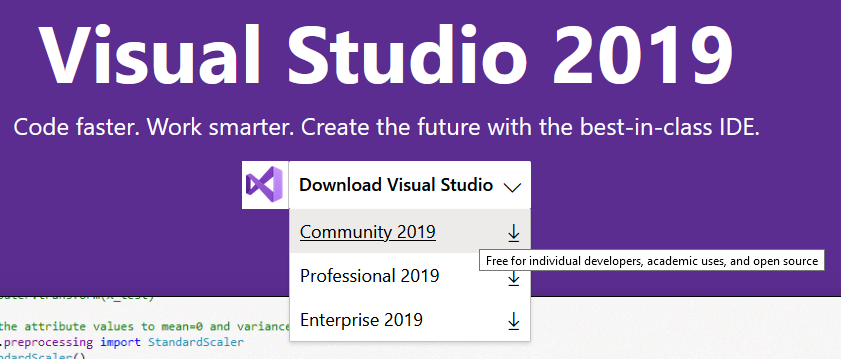
\includegraphics[scale=\figscaleAA]{images/000Adownloadcommunity}
\caption{Downloaden van Community-editie.}
\label{fig:000Adownloadcommunity}
\end{figure}


Er wordt nu een kleine installer gedownload. Start daarna de installer. Visual Studio is een groot programma, dus het kost nogal wat tijd om Visual Studio te installeren.

Visual Studio ondersteunt het ontwikkelen van applicaties met een veelzijdigheid aan mogelijkheden. Wij gebruiken de C/C++-compiler voor Desktop Development. Om te kunnen ontwikkelen moeten we een \textsl{workload} installeren. Selecteer de workload zoals te zien is in figuur~\ref{fig:000installworkload}. Selecteer de opties zoals is aangegeven aan de rechterkant van de figuur. Klik daarna op \texttt{Install while downloading}.

%\begin{figure}[H]
%\centering
%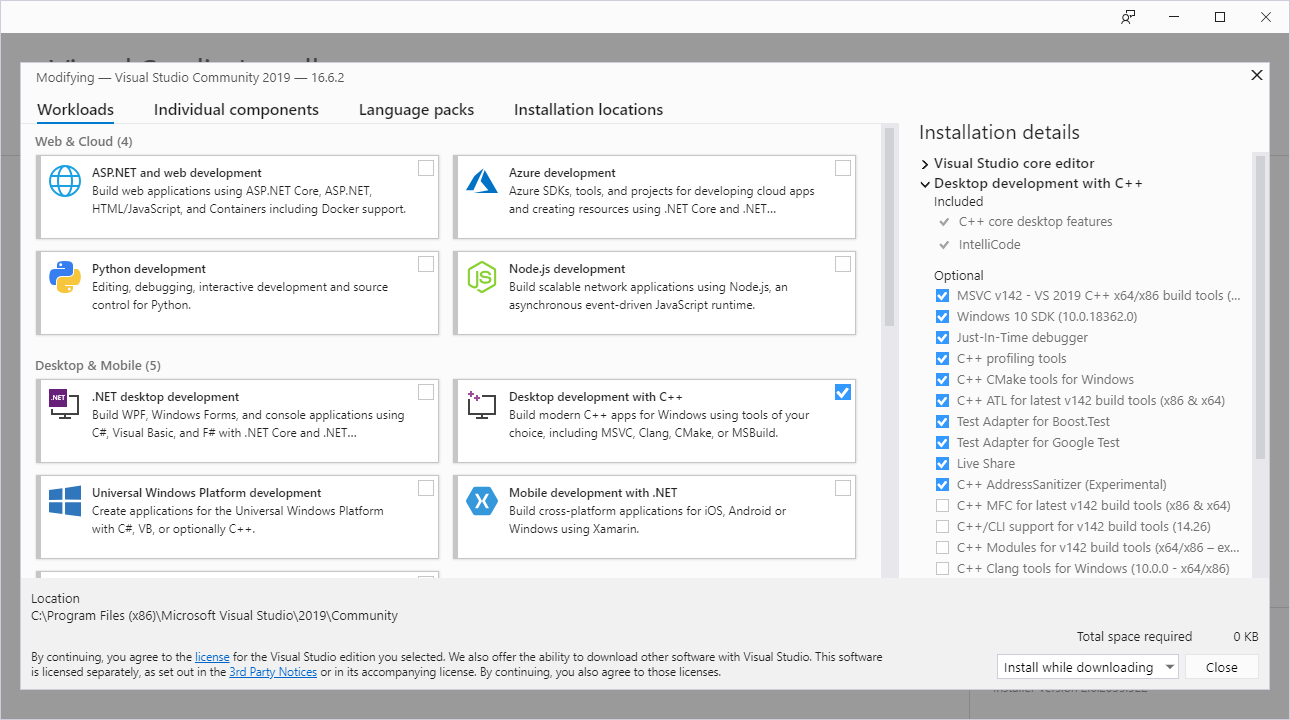
\includegraphics[scale=\figscaleAA]{images/000installworkload}
%\caption{Selecteren van de C++-workload.}
%\label{fig:000installworkload}
%\end{figure}

\begin{figure}[H]
\centering
\begin{tikzpicture}
\node[inner sep=0pt] (A) at (0,0) {
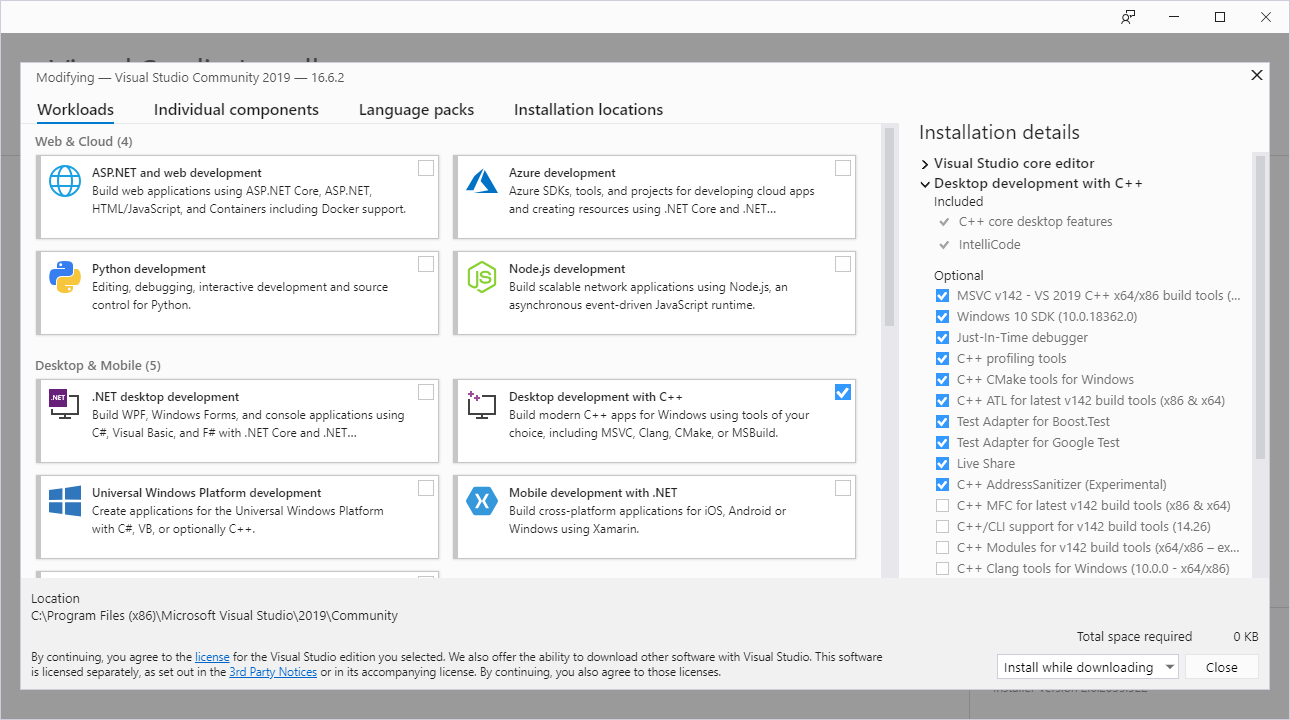
\includegraphics[width=\textwidth]{images/000installworkload}};
\draw[red,thick,rounded corners=5pt] (-2.25,-1.25) rectangle ++(4.75,1.1);
\end{tikzpicture}
\caption{Selecteren van de C++-workload.}
\label{fig:000installworkload}
\end{figure}

Start Visual Studio door op het icoon te klikken. Visual Studio opent een beginscherm waarin een nieuw project kan worden aangemaakt. Dit is te zien in figuur~\ref{fig:001newproject}. Klik op het kader \texttt{Create a new project}.

\begin{figure}[H]
\centering
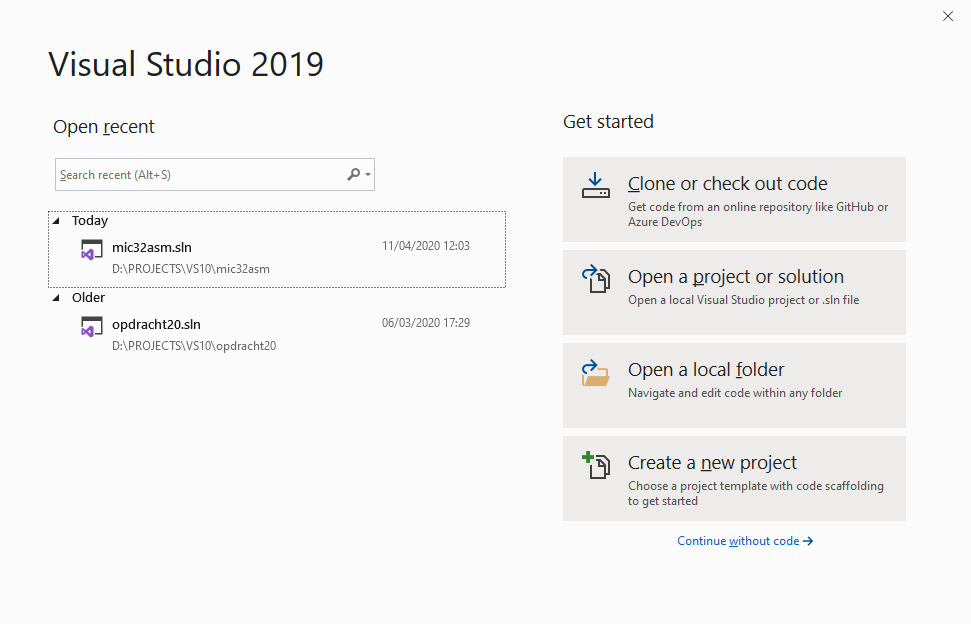
\includegraphics[scale=\figscaleH]{images/001newproject}
\caption{Aanmaken van een nieuw project.}
\label{fig:001newproject}
\end{figure}

Er wordt een nieuw scherm geopend, zie figuur~\ref{fig:002create}. Klik daarin op het kader \texttt{Empty Project}. \textbf{Klik niet op\texttt{ Console App}.}

\begin{figure}[H]
\centering
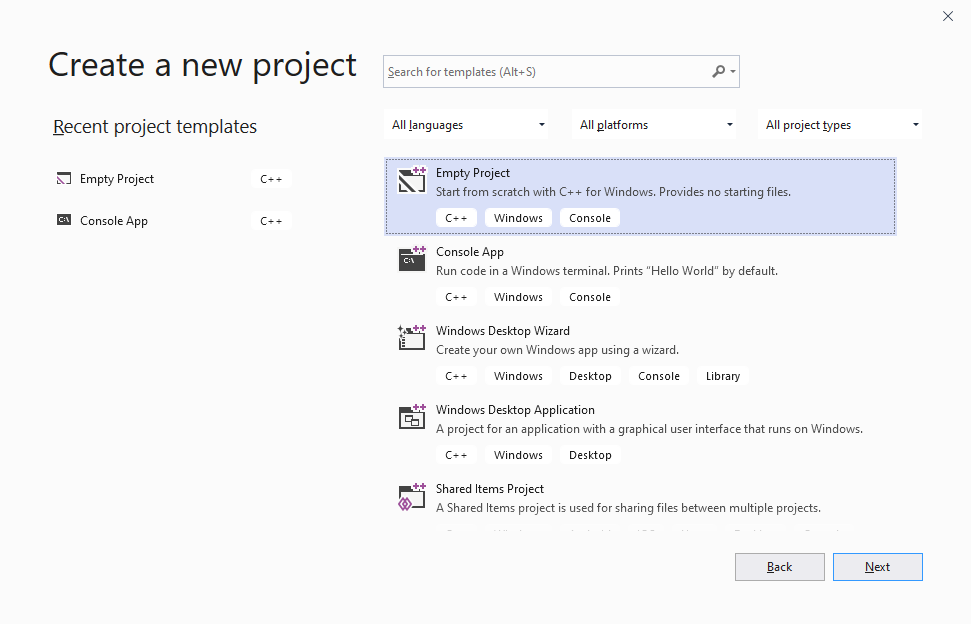
\includegraphics[scale=\figscaleH]{images/002create}
\caption{Aanmaken van een leeg project.}
\label{fig:002create}
\end{figure}

Daarna moeten wat gegevens worden ingevuld. Vul de projectnaam in en de map waarin het project terecht moet komen. Vink de checkbox onderaan aan en klik op de knop \texttt{Create}. Zie figuur~\ref{fig:003configure}.

\begin{figure}[H]
\centering
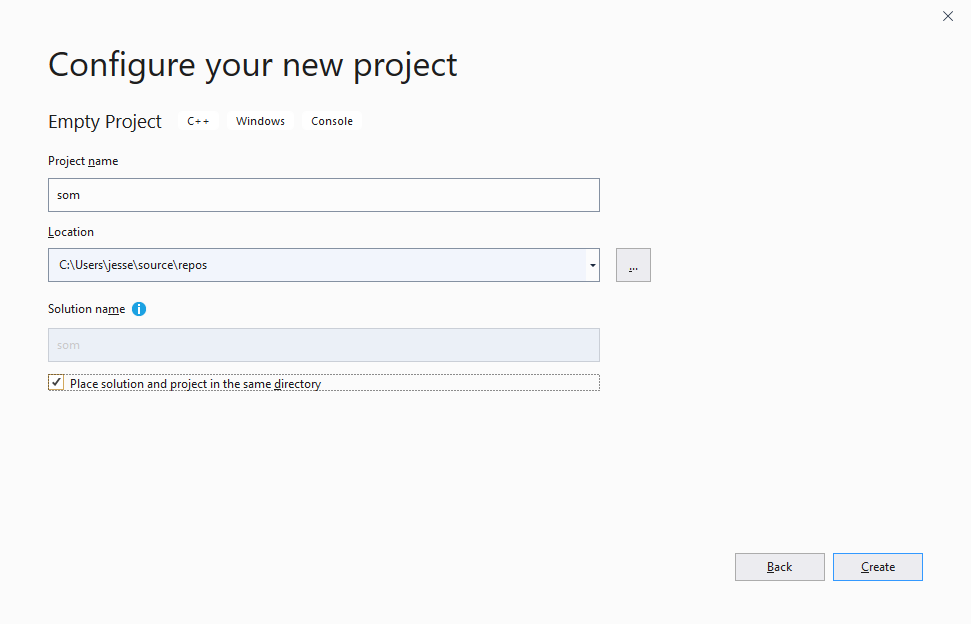
\includegraphics[scale=\figscaleH]{images/003configure}
\caption{Gegevens van het project invoeren.}
\label{fig:003configure}
\end{figure}

Visual Studio komt nu met het hoofdscherm waarin een aantal vensters (Engels: pane) te zien zijn. Er is nog geen C-bestand aangemaakt, dat moeten we zelf doen. In de \textsl{Solution Explorer} aan de rechterkant is een map \texttt{Source Files} te zien. Ga met de muis-pointer daar op staan en klik op de \textbf{rechter} muisknop.

Selecteer daarna de optie \texttt{Add} en daarna \texttt{New item..}. Zie figuur~\ref{fig:004addnewitem}.

\begin{figure}[H]
\centering
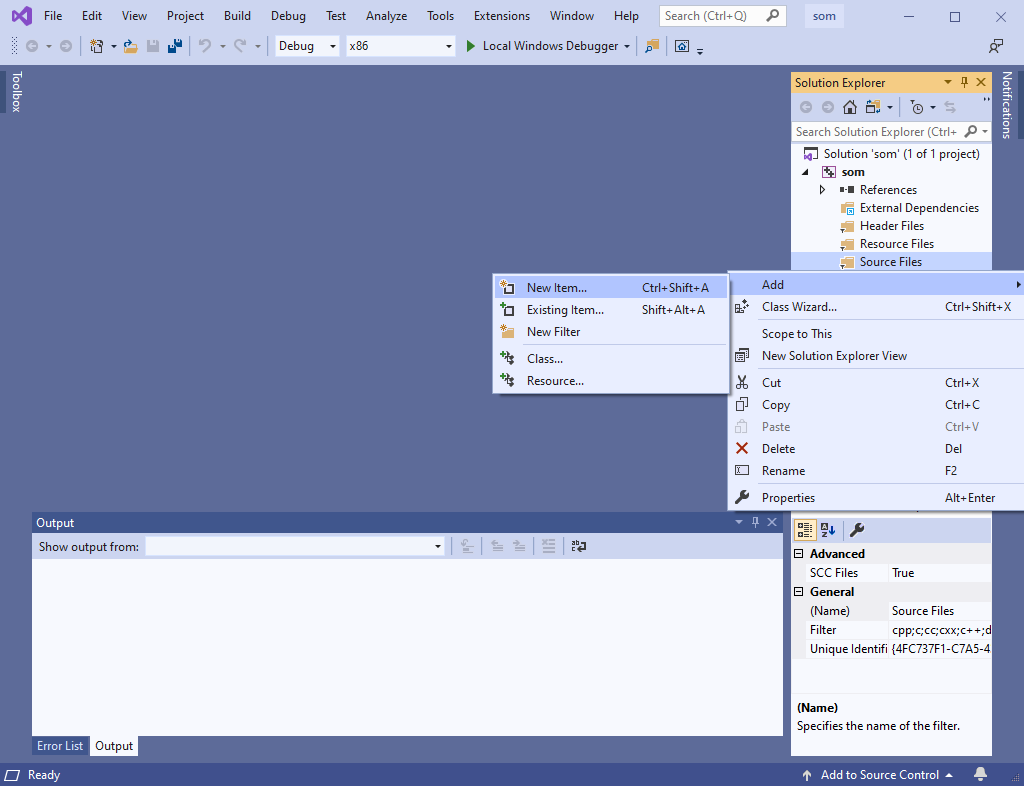
\includegraphics[scale=\figscaleH]{images/004addnewitem}
\caption{Een nieuw bestand aanmaken.}
\label{fig:004addnewitem}
\end{figure}

In het volgende scherm moet een bestandstype en een naam worden opgegeven. Klik op \texttt{C++ File (.cpp)}. Vul onderin bij  \texttt{Name} de naam van het bestand in \textbf{en zorg ervoor dat de naam eindigt met \texttt{.c}}, anders wordt een C++-bestand aangemaakt. Klik daarna op de knop \texttt{Add}. Zie figuur~\ref{fig:005enterfilename}.

Voer het programma in zoals te zien is in figuur~\ref{fig:006build}. Klik daarna op de knop \texttt{Local Windows Debugger}. Het programma wordt nu gecompileerd en als er geen fouten zijn gevonden, wordt het programma uitgevoerd. Herstel eventuele fouten die door de compiler gevonden worden en herstart de compilatie.

Het programma drukt de regel \texttt{De som van 3 en 7 is 10} af. Dit wordt gedaan in een zogenoemde \textsl{console}. Dit is te zien in figuur~\ref{fig:007output}.

De tutorial is hiermee ten einde.

\begin{figure}[H]
\centering
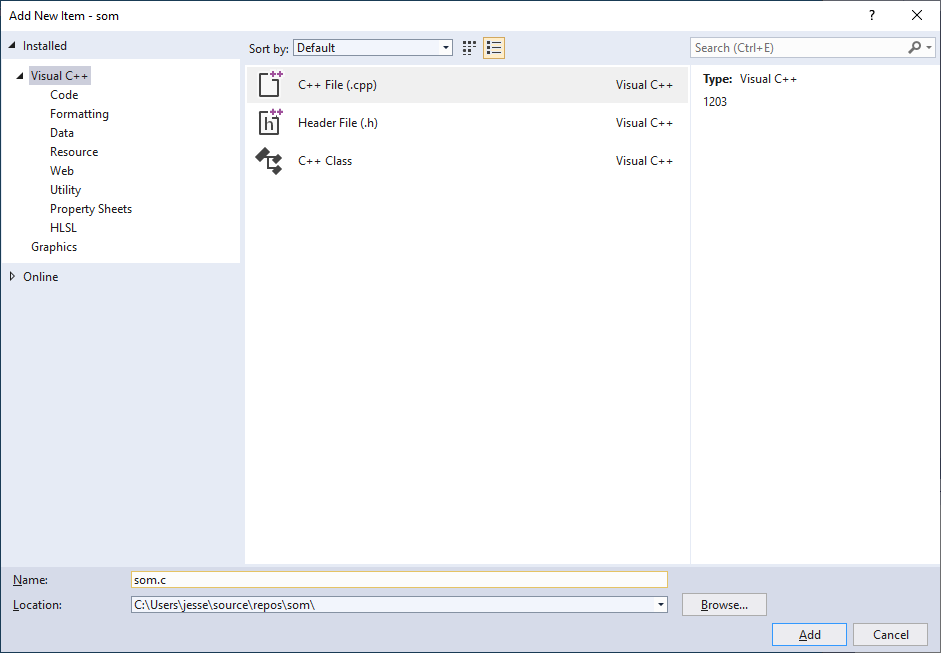
\includegraphics[scale=\figscaleH]{images/005enterfilename}
\caption{Gegevens van het C-bestand invullen.}
\label{fig:005enterfilename}
\end{figure}

\begin{figure}[H]
\centering
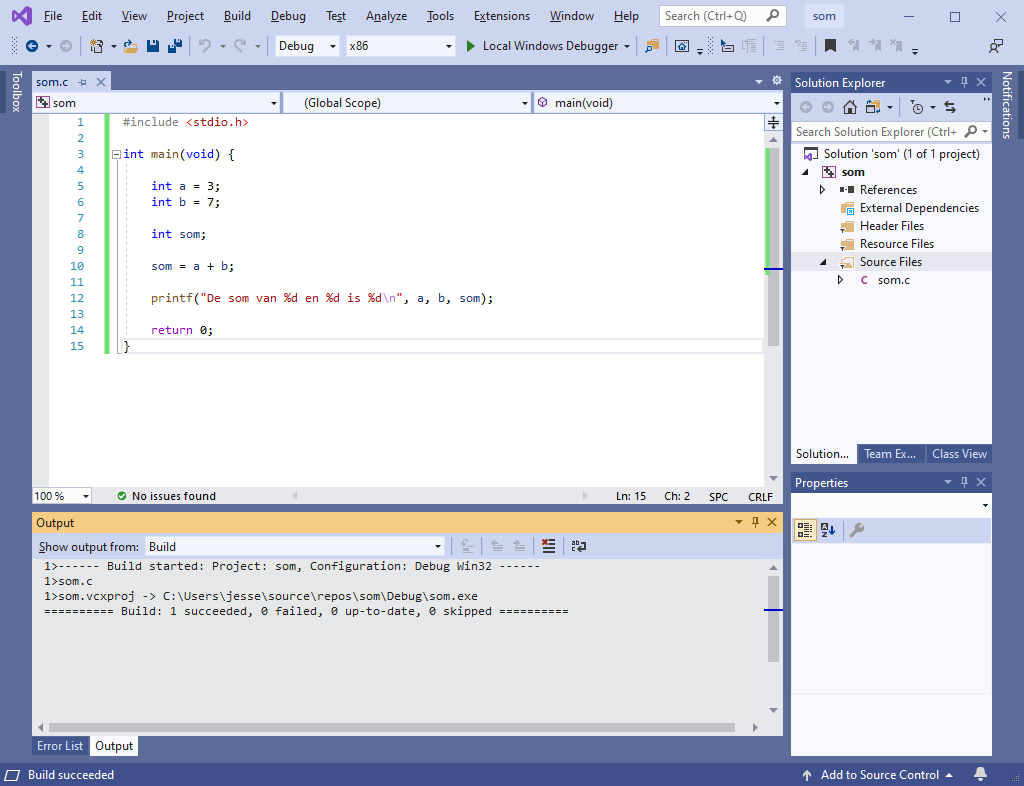
\includegraphics[scale=\figscaleH]{images/006build}
\caption{Compileren en starten van de executable.}
\label{fig:006build}
\end{figure}

\begin{figure}[H]
\centering
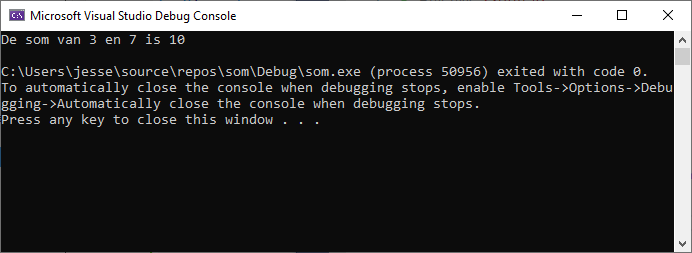
\includegraphics[scale=\figscaleH]{images/007output}
\caption{Uitvoer van het programma in een console.}
\label{fig:007output}
\end{figure}
\chapter{Voorrangsregels van operatoren}
\label{cha:voorrang}
In deze tabel zijn alle operatoren in C opgesomd. De voorrang of prioriteit is in aflopende volgorde van hoog naar laag. Twee opmerkelijke operatoren zijn (\textsl{type cast}) en \texttt{sizeof}. Bij (\textsl{type cast}) wordt het casten van een enkelvoudig datatype bedoeld, \texttt{sizeof} berekent de grootte in bytes van een datatype of variabele tijdens \textsl{compile time}\index{compile time}.

\begin{table}[!ht]
\centering
\renewcommand{\arraystretch}{1.2}
\caption{Voorrangsregels van de alle operatoren.}
\label{tab:bijvoorrangsregels}
\begin{tabular}{p{9cm}l}
\toprule
\textbf{Operator} & \textbf{Associativiteit} \\
\midrule
\texttt{() [] -> .} & links naar rechts \\
\texttt{! \textasciitilde\ + - ++ -- (}\textsl{type cast}\texttt{)} \texttt{sizeof * \&} & rechts naar links \\
\texttt{* / \%} & links naar rechts \\
\texttt{+ -} & links naar rechts \\
\texttt{<< >>} & links naar rechts\\
\texttt{< <= > >=} & links naar rechts\\
\texttt{== !=} & links naar rechts\\
\texttt{\&} & links naar rechts\\
\texttt{\^{}} & links naar rechts\\
\texttt{\textbar} & links naar rechts\\
\texttt{\&\&} & links naar rechts\\
\texttt{\textbar\textbar} & links naar rechts\\
\texttt{?:} & rechts naar links \\
\texttt{= += -= *= /= \%= \&= \^{}= \textbar= <<= >>=} & rechts naar links \\
\texttt{,} & links naar rechts \\
\bottomrule
\end{tabular}
\end{table}



%%%%%%%%%%%%%%%%%%%%%%%%%%%%%%%%%%%%%%%%%%%%%%%%%%%%%%%%%%%%%%%%%%%%%%%%%%%%%%
%
%  THE BACKMATTER
%
%%%%%%%%%%%%%%%%%%%%%%%%%%%%%%%%%%%%%%%%%%%%%%%%%%%%%%%%%%%%%%%%%%%%%%%%%%%%%%
\backmatter

% Pull in the index
%%%%%%%%%%%%%%%%%%%%%%%%%%%%%%%%%%%%%%%%%%%%%%%%%%%%%%%%%%%%%%%%%%
%%%
%%%       INDEX
%%%
%%%%%%%%%%%%%%%%%%%%%%%%%%%%%%%%%%%%%%%%%%%%%%%%%%%%%%%%%%%%%%%%%%


%% Add index to toc with clickable reference
\cleardoublepage
\phantomsection
\addcontentsline{toc}{chapter}{\indexname}
% Next doesn't work with imakeidx, use \indexsetup{othercode=\thispagestyle{fancy}}
%\thispagestyle{fancy}

\printindex


\bookbackmatter

\end{document}